\documentclass[12pt,oneside]{article}

% -------------------------------------------------
% Packages
% -------------------------------------------------
\usepackage[utf8]{inputenc}
\usepackage[T1]{fontenc}
% Libertinus has a cleaner, more open shape than the previous Palatino-style
% face and remains comfortable during long technical reading sessions.
\usepackage{libertinus}
% IBM Plex Sans gives navigation and display text a restrained technical look.
\usepackage[semibold]{plex-sans}
% A clear monospaced face keeps code distinct without looking heavy.
\usepackage[scaled=0.92]{inconsolata}
\usepackage{geometry}
\usepackage{amsmath,amssymb}
\usepackage{enumitem}
\usepackage{xcolor}
\usepackage{listings}
\usepackage{hyperref}
\usepackage{booktabs}
\usepackage{array}
\usepackage{tabularx}
\usepackage{multicol}
\usepackage{tocloft}
\usepackage{parskip}
\usepackage{microtype}
\usepackage{fancyhdr}
\usepackage{titlesec}
\usepackage{needspace}
\usepackage{placeins}
\usepackage[most]{tcolorbox}
\usepackage{tikz}
\usetikzlibrary{arrows.meta,positioning,calc,fit,backgrounds,shapes.geometric,matrix,decorations.pathreplacing}

% -------------------------------------------------
% Book Metadata
% -------------------------------------------------
\newcommand{\booktitle}{Cracking The LeetCode Interview}
\newcommand{\bookauthor}{Om Tripathi}
% Add the public repository URL after the GitHub repository is created.
\providecommand{\bookrepository}{}

% -------------------------------------------------
% Page Setup
% -------------------------------------------------
\geometry{
    paperwidth=8.5in,
    paperheight=11in,
    top=0.74in,
    bottom=0.80in,
    left=0.82in,
    right=0.82in,
    bindingoffset=0in,
    headsep=0.22in
}

% -------------------------------------------------
% Color Palette and Page Style
% -------------------------------------------------
\definecolor{navy}{HTML}{17365D}
\definecolor{teal}{HTML}{147D7E}
\definecolor{orange}{HTML}{C46B18}
\definecolor{softblue}{HTML}{EEF5FB}
\definecolor{softteal}{HTML}{EAF7F5}
\definecolor{softorange}{HTML}{FFF4E5}
\definecolor{codebackground}{HTML}{F6F8FA}
\definecolor{ink}{HTML}{243447}

\color{ink}
\setcounter{tocdepth}{1}
\setcounter{secnumdepth}{1}
\setlist[itemize]{leftmargin=1.6em,itemsep=0.25em}
\setlist[enumerate]{leftmargin=1.8em,itemsep=0.25em}
\linespread{1.025}
\setlength{\parskip}{0.48\baselineskip}
\setlength{\abovedisplayskip}{0.45em}
\setlength{\belowdisplayskip}{0.45em}
\setlength{\abovedisplayshortskip}{0.25em}
\setlength{\belowdisplayshortskip}{0.25em}
\clubpenalty=10000
\widowpenalty=10000
\displaywidowpenalty=10000
\predisplaypenalty=10000
\setlength{\emergencystretch}{2em}
\hbadness=10000
% Keep any spare space at the bottom of a page instead of stretching the
% vertical gaps between headings, paragraphs, diagrams, and code blocks.
\raggedbottom

\pagestyle{fancy}
\fancyhf{}
\fancyhead[L]{\small\textcolor{navy}{\nouppercase{\rightmark}}}
\fancyhead[R]{\small\textcolor{navy}{\booktitle}}
\fancyfoot[C]{\thepage}
\renewcommand{\headrulewidth}{0.4pt}
\setlength{\headheight}{15pt}
\renewcommand{\subsectionmark}[1]{}

% Traditional textbook contents: one readable column, strong topic divisions,
% indented lesson entries, and a quiet typographic hierarchy.
\renewcommand{\cftpartfont}{\large\plexsans\bfseries\color{navy}}
\renewcommand{\cftpartpagefont}{\large\plexsans\bfseries\color{teal}}
\renewcommand{\cftpartleader}{\hfill}
\renewcommand{\cftsecfont}{\small\color{ink}}
\renewcommand{\cftsecpagefont}{\small\plexsans\bfseries\color{navy}}
\renewcommand{\cftsecleader}{\cftdotfill{\cftdotsep}}
\setlength{\cftbeforepartskip}{0.9em}
\setlength{\cftbeforesecskip}{0.14em}
\setlength{\cftsecindent}{1.25em}
\setlength{\cftsecnumwidth}{0pt}

\makeatletter
\newcommand{\printcontentsonly}{\@starttoc{toc}}
% A code listing that needs its own page should begin at the top like a
% textbook plate, rather than being vertically centered with empty space above.
\setlength{\@fptop}{0pt}
\setlength{\@fpbot}{0pt plus 1fil}
\makeatother

\titleformat{\section}
  {\LARGE\bfseries\color{navy}\raggedright\hyphenpenalty=10000}
  {\thesection}{0.75em}{}
  [\vspace{0.2em}\color{teal}\titlerule]
\titleformat{\subsection}
  {\large\bfseries\color{navy}}
  {}{0em}{}
\titleformat{\subsubsection}
  {\normalsize\bfseries\color{teal}}
  {}{0em}{}
\titlespacing*{\section}{0pt}{0pt}{0.9em}
\titlespacing*{\subsection}{0pt}{1.15em}{0.35em}
\titlespacing*{\subsubsection}{0pt}{0.85em}{0.25em}
% Keep every heading with a substantial portion of the material that follows.
% The larger reservation also covers the opening rows of diagrams and tables,
% preventing a title from being left at the bottom of the previous page.
\pretocmd{\section}{\Needspace{12\baselineskip}}{}{}
\pretocmd{\subsection}{\Needspace{7\baselineskip}}{}{}
\pretocmd{\subsubsection}{\Needspace{5\baselineskip}}{}{}

% The code caption already names a complete solution. Suppressing the repeated
% "C++ Implementation" line prevents that line from being stranded when an
% unbreakable code block moves to the next page. Other unusually tall sections
% reserve only the amount of room their first table or paragraph needs.
\let\standardbooksubsection\subsection
\renewcommand{\subsection}[1]{%
  \ifstrequal{#1}{C++ Implementation}{}{%
    \ifstrequal{#1}{Complete Implementation}{}{%
      \ifstrequal{#1}{Complete Data Structure}{}{%
        \ifstrequal{#1}{Pseudocode}{\Needspace{14\baselineskip}}{}%
        \ifstrequal{#1}{Common judge definitions}{\Needspace{30\baselineskip}}{}%
        \ifstrequal{#1}{Detailed Table Walkthrough}{\Needspace{22\baselineskip}}{}%
        \ifstrequal{#1}{Detailed Grouping Walkthrough}{\Needspace{22\baselineskip}}{}%
        \standardbooksubsection{#1}}}}}

% -------------------------------------------------
% Hyperlink Setup
% -------------------------------------------------
\hypersetup{
    colorlinks=true,
    linkcolor=navy,
    urlcolor=teal,
    citecolor=teal,
    pdftitle={Cracking The LeetCode Interview},
    pdfauthor={Om Tripathi},
    pdfsubject={Visual C++ lessons for data structures, algorithms, and coding interviews},
    pdfkeywords={C++, algorithms, data structures, coding interviews, problem solving}
}

% -------------------------------------------------
% Code Listing Setup
% -------------------------------------------------
\lstset{
    language=C++,
    basicstyle=\ttfamily\small,
    keywordstyle=\color{navy}\bfseries,
    commentstyle=\color{teal!75!black}\itshape,
    stringstyle=\color{orange!85!black},
    numbers=left,
    numberstyle=\footnotesize\color{ink!55},
    stepnumber=1,
    numbersep=8pt,
    showstringspaces=false,
    breaklines=true,
    breakindent=1.4em,
    prebreak=\mbox{\textcolor{orange}{\scriptsize$\hookleftarrow$}},
    postbreak=\mbox{\textcolor{orange}{\scriptsize$\hookrightarrow$}\space},
    frame=leftline,
    framerule=1.1pt,
    rulecolor=\color{teal},
    backgroundcolor=\color{codebackground},
    tabsize=4,
    columns=fullflexible,
    keepspaces=true,
    xleftmargin=1.2em,
    framexleftmargin=0.6em,
    aboveskip=0.65em,
    belowskip=0.65em,
    captionpos=t
}

\lstdefinestyle{pseudocode}{
    language={},
    basicstyle=\ttfamily\small,
    numbers=none,
    frame=leftline,
    framerule=1.1pt,
    rulecolor=\color{orange},
    backgroundcolor=\color{softorange!55},
    xleftmargin=1.2em,
    framexleftmargin=0.6em,
    columns=fullflexible,
    keepspaces=true,
    showstringspaces=false
}

% Use a plain book-friendly caption name. "Code" is clearer to new readers
% than LaTeX's default word "Listing".
\renewcommand{\lstlistingname}{Code}

% Complete solutions use a clearly readable textbook code size while remaining
% compact enough for the usual interview-length method to stay together.
\lstdefinestyle{compactcode}{
    basicstyle=\ttfamily\small,
    numbers=left,
    numberstyle=\scriptsize\color{ink!55},
    aboveskip=0.5em,
    belowskip=0.5em
}

% A few complete classes are much longer than the usual judge method.
% They use this smaller style so the whole class can stay on one page.
\lstdefinestyle{longcode}{
    basicstyle=\ttfamily\footnotesize,
    numbers=left,
    numberstyle=\scriptsize\color{ink!55},
    numbersep=5pt,
    xleftmargin=0.9em,
    framexleftmargin=0.45em,
    aboveskip=0.4em,
    belowskip=0.4em
}

% -------------------------------------------------
% Custom Commands
% -------------------------------------------------
\newcommand{\Oof}[1]{O(#1)}
\newcommand{\inlinecode}[1]{\texttt{#1}}
% The judge workflow is explained once in the introduction. Keeping this
% compatibility command empty avoids repeating the same note after every
% solution.
\newcommand{\judgeclassnote}{}

\newtcolorbox{conceptbox}[1]{
    enhanced,
    breakable,
    colback=softblue,
    colframe=navy,
    boxrule=0.7pt,
    arc=2mm,
    title=\textbf{#1},
    fonttitle=\color{white},
    colbacktitle=navy,
    attach boxed title to top left={xshift=4mm,yshift=-2mm},
    boxed title style={arc=1.5mm}
}

\newtcolorbox{dryrunbox}[1]{
    enhanced,
    colback=softorange,
    colframe=orange,
    boxrule=0.7pt,
    arc=2mm,
    title=\textbf{#1},
    fonttitle=\color{white},
    colbacktitle=orange,
    before skip=1.1em,
    after skip=1.1em
}

\newtcolorbox{visualbox}[1]{
    enhanced,
    colback=white,
    colframe=teal,
    boxrule=0.9pt,
    arc=2mm,
    title=\textbf{#1},
    fonttitle=\color{white},
    colbacktitle=teal,
    before skip=1.1em,
    after skip=1.1em
}

\BeforeBeginEnvironment{visualbox}{\par\Needspace{8\baselineskip}}
\BeforeBeginEnvironment{dryrunbox}{\par\Needspace{8\baselineskip}}
\BeforeBeginEnvironment{conceptbox}{\par\Needspace{6\baselineskip}}
\BeforeBeginEnvironment{invariantbox}{\par\Needspace{6\baselineskip}}
\BeforeBeginEnvironment{revisionbox}{\par\Needspace{6\baselineskip}}
% Short pseudocode blocks should stay with their heading. Complete solutions
% may split cleanly at a page boundary instead of forcing large blank areas.
\BeforeBeginEnvironment{lstlisting}{\par\Needspace{8\baselineskip}}

\newtcolorbox{problemcard}[1]{
    enhanced,
    colback=softblue,
    colframe=navy,
    boxrule=0.8pt,
    arc=2mm,
    title=\textbf{Problem at a glance},
    colbacktitle=navy,
    coltitle=white,
    fonttitle=\bfseries,
    before skip=0.8em,
    after skip=1.2em,
    #1
}

\newcommand{\problemprofile}[3]{%
\begin{problemcard}{}
\begin{tabularx}{\linewidth}{@{}X X X@{}}
\textcolor{teal}{\textbf{Difficulty}} &
\textcolor{teal}{\textbf{Approach}} &
\textcolor{teal}{\textbf{Main tool}}\\[-1mm]
\textbf{#1} & #2 & #3
\end{tabularx}
\end{problemcard}}

\newcounter{lesson}
\newcommand{\currentpattern}{Interview Foundations}
\newcommand{\problemstart}[5]{%
\FloatBarrier
\par\Needspace{22\baselineskip}
\refstepcounter{lesson}%
\phantomsection
{\plexsans\small\bfseries\color{teal}\MakeUppercase{\currentpattern}\par}
\vspace{0.3em}
\section*{Lesson \thelesson: #1}
\label{lesson:\thelesson}
\addcontentsline{toc}{section}{Lesson \thelesson: #1}
\markboth{#1}{#4}
\problemprofile{#3}{#4}{#5}}

\newcommand{\patternintoc}[1]{%
  \gdef\currentpattern{#1}%
  \phantomsection
  \addtocontents{toc}{\protect\Needspace{4\baselineskip}}%
  \addcontentsline{toc}{part}{#1}}

\newtcolorbox{revisionbox}[1]{
  enhanced,breakable,colback=softteal,colframe=teal,boxrule=0.8pt,
  arc=2mm,title=\textbf{#1},colbacktitle=teal,coltitle=white,
  before skip=0.8em,after skip=0.8em
}

\newtcolorbox{invariantbox}[1]{
  enhanced,breakable,colback=softblue,colframe=navy,boxrule=0.8pt,
  arc=2mm,title=\textbf{Key idea: #1},colbacktitle=navy,coltitle=white,
  before skip=0.8em,after skip=0.8em
}

% Real data-structure dry runs.  These drawings show the object that changes;
% they do not use prose-filled process boxes as a substitute for a visual.
\newcommand{\arraydryvisual}{%
\begin{visualbox}{Array example: two positions move through the row}\centering
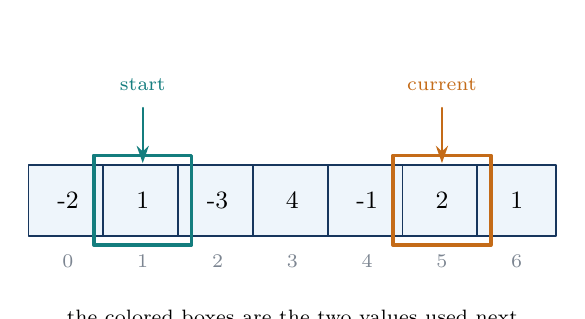
\begin{tikzpicture}[font=\scriptsize,>={Stealth[length=2.2mm,width=1.55mm]}]
  \foreach \v [count=\i from 0] in {-2,1,-3,4,-1,2,1}{
    \node[arraycell] (a\i) at (.95*\i,0) {\v};
    \node[below=1mm of a\i,font=\scriptsize,text=ink!60]{\i};}
  \node[draw=teal,very thick,fit=(a1),inner sep=1mm]{};
  \node[draw=orange,very thick,fit=(a5),inner sep=1mm]{};
  \draw[flowarrow,teal] ([yshift=7mm]a1.north)--(a1.north);
  \draw[flowarrow,orange] ([yshift=7mm]a5.north)--(a5.north);
  \node[above=8mm of a1,text=teal]{start};
  \node[above=8mm of a5,text=orange]{current};
  \node[below=8mm of a3]{the colored boxes are the two values used next};
\end{tikzpicture}\end{visualbox}}

\newcommand{\stringdryvisual}{%
\begin{visualbox}{String example: the checked section grows and shrinks}\centering
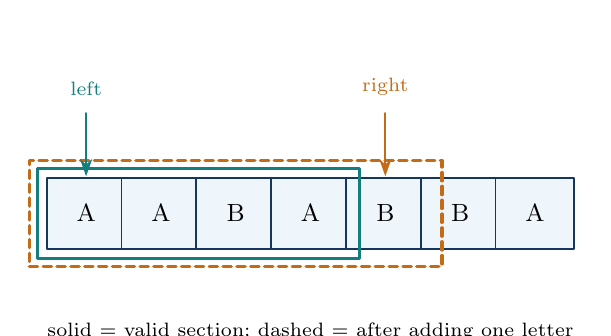
\begin{tikzpicture}[font=\scriptsize,>={Stealth[length=2.2mm,width=1.55mm]}]
  \foreach \v [count=\i from 0] in {A,A,B,A,B,B,A}{
    \node[arraycell] (s\i) at (.95*\i,0) {\v};}
  \node[draw=teal,very thick,fit=(s0)(s3),inner sep=1mm]{};
  \node[draw=orange,very thick,densely dashed,fit=(s0)(s4),inner sep=2mm]{};
  \draw[flowarrow,teal] ([yshift=8mm]s0.north)--(s0.north);
  \draw[flowarrow,orange] ([yshift=8mm]s4.north)--(s4.north);
  \node[above=9mm of s0,text=teal]{left};
  \node[above=9mm of s4,text=orange]{right};
  \node[below=8mm of s3]{solid = valid section; dashed = after adding one letter};
\end{tikzpicture}\end{visualbox}}

\newcommand{\hashdryvisual}{%
\begin{visualbox}{Hash table example: save a value, then find it}\centering
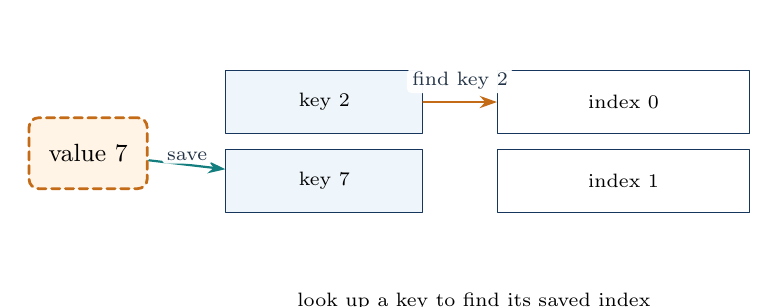
\begin{tikzpicture}[font=\scriptsize,>={Stealth[length=2.2mm,width=1.55mm]}]
  \node[dsnode,active] (in) at (-3,0) {value 7};
  \node[draw=navy,fill=softblue,minimum width=25mm,minimum height=8mm] (k1) at (0,.65) {key 2};
  \node[draw=navy,minimum width=32mm,minimum height=8mm] (v1) at (3.8,.65) {index 0};
  \node[draw=navy,fill=softblue,minimum width=25mm,minimum height=8mm] (k2) at (0,-.35) {key 7};
  \node[draw=navy,minimum width=32mm,minimum height=8mm] (v2) at (3.8,-.35) {index 1};
  \draw[flowarrow,teal] (in)--node[edgelabel,above]{save} (k2);
  \draw[flowarrow,orange] (k1)--node[edgelabel,above=1mm]{find key 2} (v1);
  \node[below=9mm of k2,xshift=19mm]{look up a key to find its saved index};
\end{tikzpicture}\end{visualbox}}

\newcommand{\listdryvisual}{%
\begin{visualbox}{Reverse one link: make 3 point back to 2}\centering
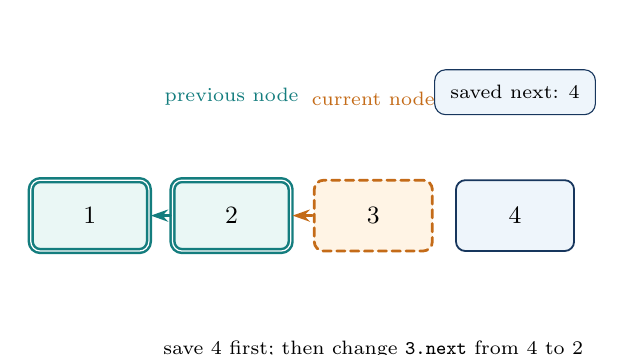
\begin{tikzpicture}[font=\scriptsize,>={Stealth[length=2.2mm,width=1.55mm]}]
  \node[dsnode,visited] (l0) at (0,0) {1};
  \node[dsnode,visited] (l1) at (1.8,0) {2};
  \node[dsnode,active] (l2) at (3.6,0) {3};
  \node[dsnode] (l3) at (5.4,0) {4};
  \draw[flowarrow,teal] (l1.west)--(l0.east);
  \draw[flowarrow,orange] (l2.west)--(l1.east);
  \node[above=8mm of l1,text=teal]{previous node};
  \node[above=8mm of l2,text=orange]{current node};
  \node[above=8mm of l3,draw=navy,fill=softblue,rounded corners,
    inner sep=2mm] {saved next: 4};
  \node[below=10mm of l2]{save 4 first; then change \texttt{3.next} from 4 to 2};
\end{tikzpicture}\end{visualbox}}

\newcommand{\cycledryvisual}{%
\begin{visualbox}{Fast catches slow inside the loop}\centering
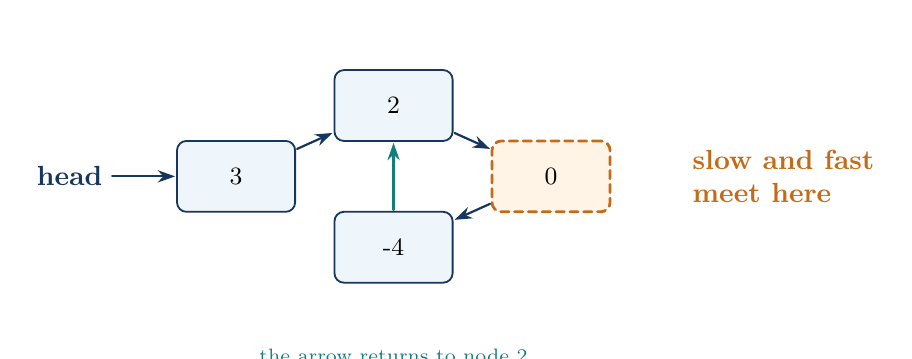
\begin{tikzpicture}[font=\scriptsize,>={Stealth[length=2.2mm,width=1.55mm]}]
  \node[dsnode] (c0) at (0,0) {3};
  \node[dsnode] (c1) at (2.0,0.9) {2};
  \node[dsnode,active] (c2) at (4.0,0) {0};
  \node[dsnode] (c3) at (2.0,-0.9) {-4};
  \draw[flowarrow] (c0)--(c1);
  \draw[flowarrow] (c1)--(c2);
  \draw[flowarrow] (c2)--(c3);
  \draw[flowarrow,teal] (c3)--(c1);
  \node[left=8mm of c0,text=navy,font=\bfseries] (head) {head};
  \draw[flowarrow] (head)--(c0);
  \node[right=9mm of c2,align=left,text=orange,font=\bfseries]
    {slow and fast\\meet here};
  \node[below=7mm of c3,text=teal]{the arrow returns to node 2};
\end{tikzpicture}\end{visualbox}}

\newcommand{\stackdryvisual}{%
\begin{visualbox}{Stack dry run: the top item is handled first}\centering
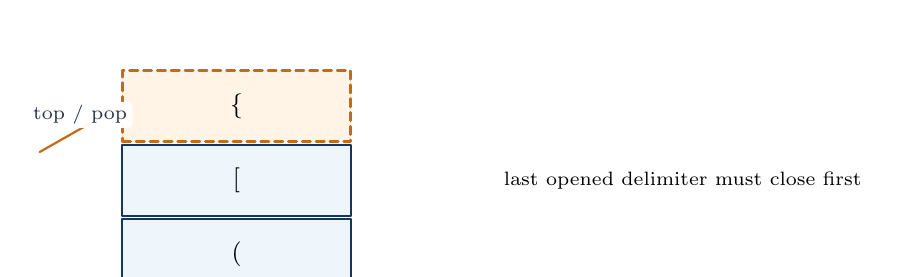
\begin{tikzpicture}[font=\scriptsize,>={Stealth[length=2.2mm,width=1.55mm]}]
  \node[arraycell,minimum width=29mm] (x0) {(};
  \node[arraycell,minimum width=29mm,above=0mm of x0] (x1) {[};
  \node[arraycell,minimum width=29mm,above=0mm of x1,active] (x2) {\{};
  \draw[flowarrow,orange] (-2.5,1.3)--node[edgelabel,above]{top / pop} (x2.west);
  \node[right=18mm of x1]{last opened delimiter must close first};
\end{tikzpicture}\end{visualbox}}

\newcommand{\queuedryvisual}{%
\begin{visualbox}{Queue example: handle one tree level at a time}\centering
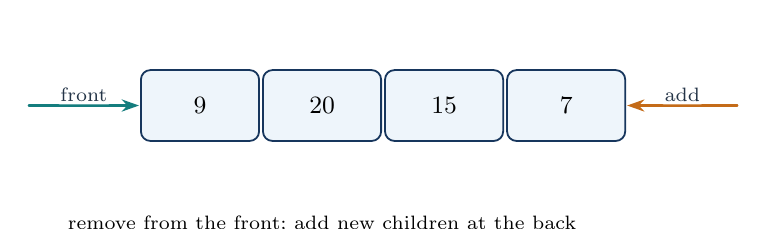
\begin{tikzpicture}[font=\scriptsize,>={Stealth[length=2.2mm,width=1.55mm]}]
  \foreach \v [count=\i from 0] in {9,20,15,7}{\node[dsnode] (q\i) at (1.55*\i,0){\v};}
  \draw[flowarrow,teal] ([xshift=-14mm]q0.west)--node[edgelabel,above]{front} (q0.west);
  \draw[flowarrow,orange] ([xshift=14mm]q3.east)--node[edgelabel,above]{add} (q3.east);
  \node[below=8mm of q1]{remove from the front; add new children at the back};
\end{tikzpicture}\end{visualbox}}

\newcommand{\treedryvisual}{%
\begin{visualbox}{Tree example: child answers move up to the parent}\centering
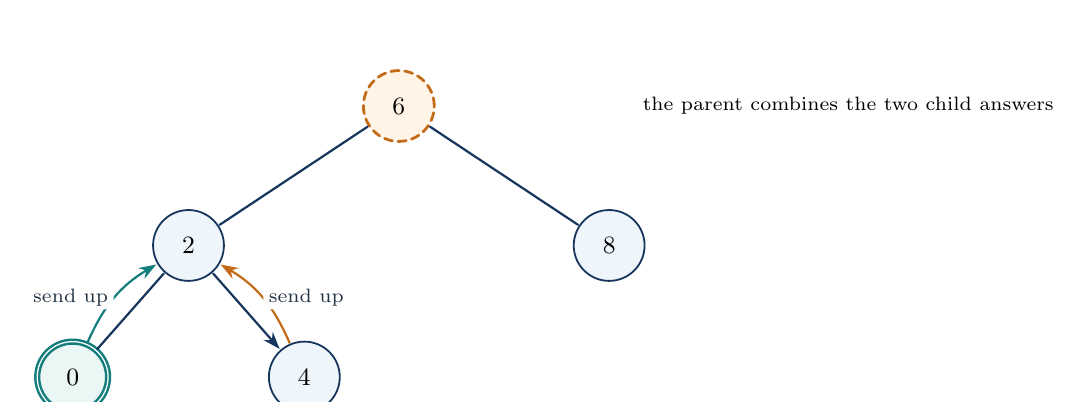
\begin{tikzpicture}[font=\scriptsize,>={Stealth[length=2.2mm,width=1.55mm]}]
  \node[trienode,active] (r) {6};
  \node[trienode,below left=11mm and 20mm of r] (l) {2};
  \node[trienode,below right=11mm and 20mm of r] (rr) {8};
  \node[trienode,visited,below left=10mm and 8mm of l] (ll) {0};
  \node[trienode,below right=10mm and 8mm of l] (lr) {4};
  \draw[flowarrow] (r)--(l) (r)--(rr) (l)--(ll) (l)--(lr);
  \draw[flowarrow,teal] (ll) to[bend left=18] node[edgelabel,left]{send up} (l);
  \draw[flowarrow,orange] (lr) to[bend right=18] node[edgelabel,right]{send up} (l);
  \node[right=25mm of r]{the parent combines the two child answers};
\end{tikzpicture}\end{visualbox}}

\newcommand{\heapdryvisual}{%
\begin{visualbox}{Heap example: the next value stays on top}\centering
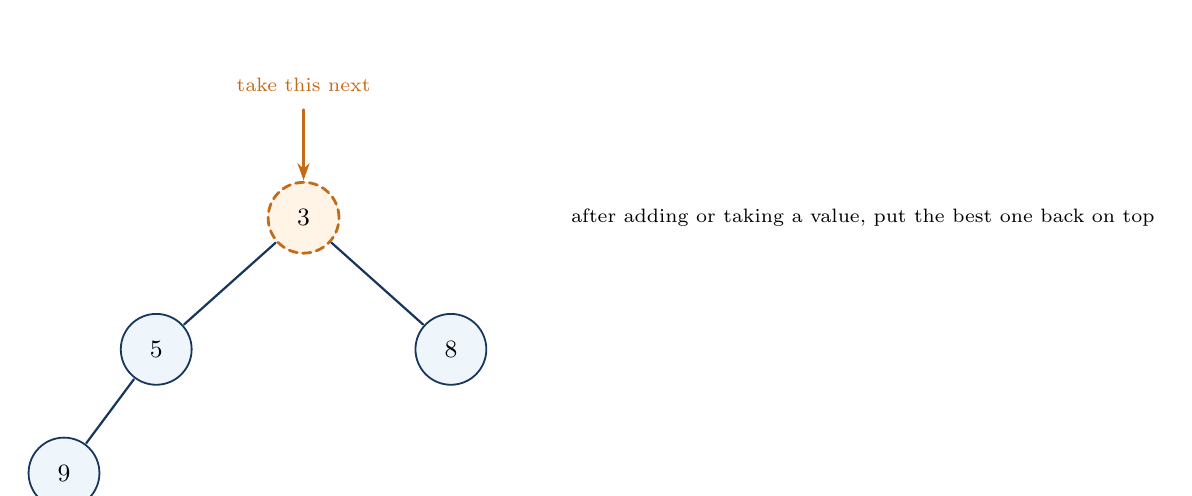
\begin{tikzpicture}[font=\scriptsize,>={Stealth[length=2.2mm,width=1.55mm]}]
  \node[trienode,active] (h0) {3};
  \node[trienode,below left=10mm and 12mm of h0] (h1) {5};
  \node[trienode,below right=10mm and 12mm of h0] (h2) {8};
  \node[trienode,below left=9mm and 5mm of h1] (h3) {9};
  \draw[-,thick,navy] (h0)--(h1) (h0)--(h2) (h1)--(h3);
  \draw[flowarrow,orange] ([yshift=9mm]h0.north)--(h0.north);
  \node[above=10mm of h0,text=orange]{take this next};
  \node[right=28mm of h0]{after adding or taking a value, put the best one back on top};
\end{tikzpicture}\end{visualbox}}

\newcommand{\graphdryvisual}{%
\begin{visualbox}{Graph example: mark a node so it is not visited twice}\centering
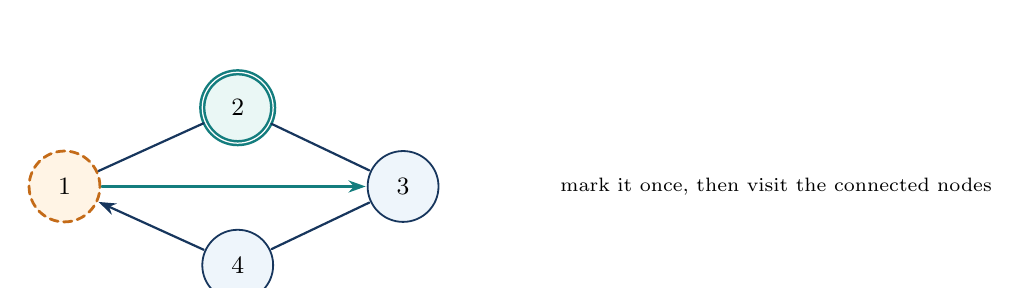
\begin{tikzpicture}[font=\scriptsize,>={Stealth[length=2.2mm,width=1.55mm]}]
  \node[trienode,active] (g0) at (0,1){1};
  \node[trienode,visited] (g1) at (2.2,2){2};
  \node[trienode] (g2) at (4.3,1){3};
  \node[trienode] (g3) at (2.2,0){4};
  \draw[flowarrow] (g0)--(g1)--(g2)--(g3)--(g0);
  \draw[flowarrow,teal] (g0)--(g2);
  \node[right=14mm of g2]{mark it once, then visit the connected nodes};
\end{tikzpicture}\end{visualbox}}

\newcommand{\triedryvisual}{%
\begin{visualbox}{Trie example: follow one letter at a time}\centering
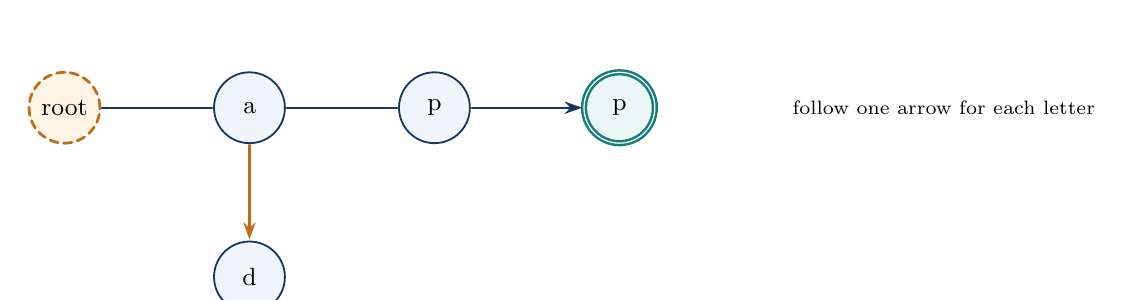
\begin{tikzpicture}[font=\scriptsize,>={Stealth[length=2.2mm,width=1.55mm]}]
  \node[trienode,active] (t0) {root};
  \node[trienode,right=14mm of t0] (t1) {a};
  \node[trienode,right=14mm of t1] (t2) {p};
  \node[trienode,right=14mm of t2,visited] (t3) {p};
  \node[trienode,below=12mm of t1] (tb) {d};
  \draw[flowarrow] (t0)--(t1)--(t2)--(t3);
  \draw[flowarrow,orange] (t1)--(tb);
  \node[right=16mm of t3]{follow one arrow for each letter};
\end{tikzpicture}\end{visualbox}}

\newcommand{\griddryvisual}{%
\begin{visualbox}{Grid / DP dry run: each cell has visible neighbors}\centering
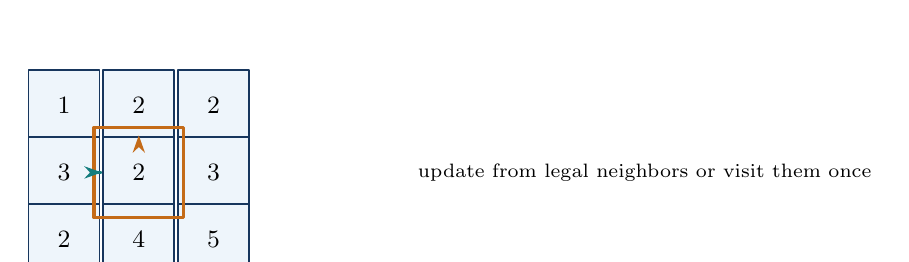
\begin{tikzpicture}[font=\scriptsize,>={Stealth[length=2.2mm,width=1.55mm]}]
  \foreach \v [count=\k from 0] in {1,2,2,3,2,3,2,4,5}{
    \pgfmathtruncatemacro{\r}{int(\k/3)}\pgfmathtruncatemacro{\c}{mod(\k,3)}
    \node[arraycell,minimum width=9mm] (m\r\c) at (.95*\c,-.85*\r){\v};}
  \node[draw=orange,very thick,fit=(m11),inner sep=1mm]{};
  \draw[flowarrow,teal] (m10)--(m11);
  \draw[flowarrow,orange] (m01)--(m11);
  \node[right=20mm of m12]{update from legal neighbors or visit them once};
\end{tikzpicture}\end{visualbox}}

\newcommand{\intervaldryvisual}{%
\begin{visualbox}{Interval dry run: compare start with the active end}\centering
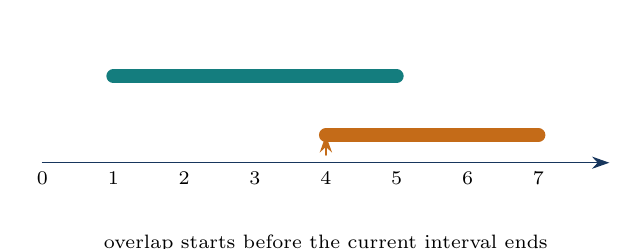
\begin{tikzpicture}[font=\scriptsize,>={Stealth[length=2.2mm,width=1.55mm]},x=9mm]
  \draw[->,navy] (0,0)--(8,0);
  \draw[line width=5pt,teal] (1,1.1)--(5,1.1);
  \draw[line width=5pt,orange] (4,.35)--(7,.35);
  \foreach \x in {0,...,7}\node[below] at (\x,0){\scriptsize\x};
  \draw[flowarrow,orange] (4,.1)--(4,.35);
  \node[below=8mm] at (4,0){overlap starts before the current interval ends};
\end{tikzpicture}\end{visualbox}}

\newcommand{\bitdryvisual}{%
\begin{visualbox}{Binary example: focus on one 0 or 1 at a time}\centering
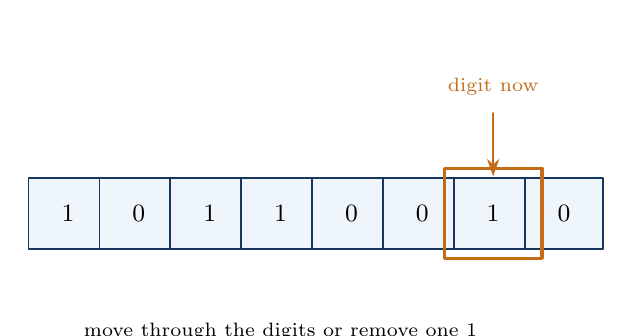
\begin{tikzpicture}[font=\scriptsize,>={Stealth[length=2.2mm,width=1.55mm]}]
  \foreach \v [count=\i from 0] in {1,0,1,1,0,0,1,0}{\node[arraycell] (b\i) at (.9*\i,0){\v};}
  \node[draw=orange,very thick,fit=(b6),inner sep=1mm]{};
  \draw[flowarrow,orange] ([yshift=8mm]b6.north)--(b6.north);
  \node[above=9mm of b6,text=orange]{digit now};
  \node[below=8mm of b3]{move through the digits or remove one 1};
\end{tikzpicture}\end{visualbox}}

\newcommand{\dpdryvisual}{%
\begin{visualbox}{Table example: use earlier answers to find the next one}\centering
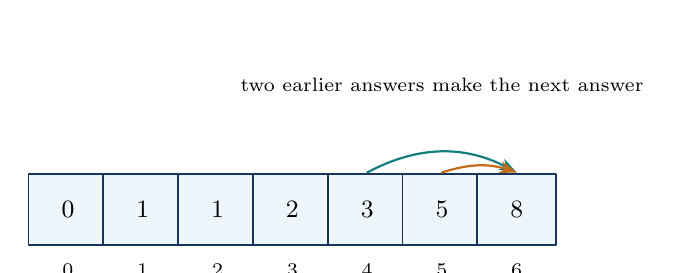
\begin{tikzpicture}[font=\scriptsize,>={Stealth[length=2.2mm,width=1.55mm]}]
  \foreach \v [count=\i from 0] in {0,1,1,2,3,5,8}{
    \node[arraycell] (d\i) at (.95*\i,0){\v};
    \node[below=1mm of d\i,font=\scriptsize]{\i};}
  \draw[flowarrow,teal] (d4.north) to[bend left=28] (d6.north);
  \draw[flowarrow,orange] (d5.north) to[bend left=18] (d6.north);
  \node[above=9mm of d5]{two earlier answers make the next answer};
\end{tikzpicture}\end{visualbox}}

% Match every lesson to the structure used by its algorithm.
\newcommand{\lessonstructurevisual}{%
\ifcase\value{lesson}\relax
\or\hashdryvisual\or\arraydryvisual\or\arraydryvisual\or\triedryvisual\or\triedryvisual
\or\graphdryvisual\or\queuedryvisual\or\treedryvisual\or\graphdryvisual\or\dpdryvisual
\or\dpdryvisual\or\treedryvisual\or\arraydryvisual\or\hashdryvisual\or\bitdryvisual
\or\graphdryvisual\or\dpdryvisual\or\cycledryvisual\or\stringdryvisual\or\heapdryvisual
\or\arraydryvisual\or\graphdryvisual\or\hashdryvisual\or\dpdryvisual\or\dpdryvisual
\or\dpdryvisual\or\dpdryvisual\or\stringdryvisual\or\stringdryvisual\or\stringdryvisual
\or\dpdryvisual\or\intervaldryvisual\or\arraydryvisual\or\treedryvisual\or\treedryvisual
\or\treedryvisual\or\heapdryvisual\or\intervaldryvisual\or\intervaldryvisual\or\intervaldryvisual
\or\griddryvisual\or\graphdryvisual\or\hashdryvisual\or\listdryvisual\or\heapdryvisual
\or\griddryvisual\or\stringdryvisual\or\bitdryvisual\or\bitdryvisual\or\arraydryvisual
\or\listdryvisual\or\listdryvisual\or\listdryvisual\or\bitdryvisual\or\griddryvisual
\or\treedryvisual\or\treedryvisual\or\griddryvisual\or\griddryvisual\or\treedryvisual
\or\bitdryvisual\or\heapdryvisual\or\griddryvisual\or\hashdryvisual\or\stringdryvisual
\or\stackdryvisual\or\treedryvisual\or\dpdryvisual\or\triedryvisual\or\griddryvisual
\or\arraydryvisual\or\dpdryvisual\or\dpdryvisual\or\treedryvisual\or\griddryvisual
\fi}

% Earlier drafts ended every lesson with another generic summary and, for the
% first lessons, a generic data-structure picture. Those blocks duplicated the
% lesson-specific revision boxes and sometimes created a nearly empty page or
% an arrow unrelated to the actual example. Keep the calls in chapter files as
% editorial metadata, but do not print the redundant template.
\newcommand{\chaptercheckpoint}[4]{}

% A shared layout for the later lessons. The text passed to this command is
% different for every problem; the headings simply keep the book consistent.
\newcommand{\lessonexpansion}[4]{%
\Needspace{20\baselineskip}
\subsection{Walk Through the Example}
% The lesson already includes a diagram made for its exact example. Repeating
% a generic array, string, or tree here can show different values and suggest
% the wrong operation, so the walkthrough continues directly with its trace.
\begin{dryrunbox}{Trace the example one update at a time}
#1
\end{dryrunbox}
\subsection{Why It Works}
#2
\begin{revisionbox}{Tests to try}
#3
\end{revisionbox}
\begin{revisionbox}{How to explain it in an interview}
#4
\end{revisionbox}%
\ifcsname sourcewalkthrough@\thelesson\endcsname
  \subsection{A Closer Look}
  \csname sourcewalkthrough@\thelesson\endcsname
\fi}

% Additional explanations for the middle group of lessons.

\expandafter\def\csname sourcewalkthrough@26\endcsname{%
A useful way to begin is to ask: what does the current sum
mean at one exact index? It is not the best sum anywhere in the array. It is
the best sum of a subarray that must end at the current value. This difference
is what makes one pass possible. If the old running sum is negative, carrying
it forward only makes the next choice worse, so the scan starts again. If it
is positive, adding the new value may continue a useful block.

For \texttt{[-2,1,-3,4,-1,2,1,-5,4]}, the running value is first \(-2\).
At 1, starting again is better than extending \(-2\), so the running value
becomes 1. The same decision happens again at 4 because the sum before it is
negative. From 4 onward, the values \(-1,2,1\) still leave a positive running
sum, so that block is kept. A separate variable stores the best running value
ever seen. Initializing both variables from the first element, rather than
zero, is important when every array value is negative.}

\expandafter\def\csname sourcewalkthrough@27\endcsname{%
Products need one more piece of state than sums. A very small negative product
can become a very large positive product after another negative number. For
that reason, the scan keeps both the largest and smallest product ending at
the current position. Neither one can be discarded early.

At every value there are three choices: start a new subarray with this value,
multiply it by the previous maximum, or multiply it by the previous minimum.
The largest candidate becomes the new maximum and the smallest becomes the
new minimum. With \texttt{[-2,3,-4]}, the states after 3 are maximum 3 and
minimum \(-6\). When \(-4\) arrives, \((-6)(-4)=24\), so the old minimum
creates the new maximum. Zero also works naturally: it can end the old block
and start a new one. Both old states must be saved before either is updated,
otherwise the second calculation may use a value from the current step.}

\expandafter\def\csname sourcewalkthrough@28\endcsname{%
The window does not need every character to match already. It only needs to
be repairable with at most \(k\) replacements. Inside a window of length
\(L\), keep the character that appears most often and replace the other
\(L-f\) positions. The window is allowed exactly when \(L-f\le k\).

As the right edge moves, update the count for the new character and the
largest frequency seen. If the replacement cost is too large, move the left
edge and remove those characters from the active counts. The stored maximum
frequency is allowed to be slightly old. It may delay a shrink, but it cannot
produce a better answer that was never possible earlier. For
\texttt{AABABBA} with \(k=1\), \texttt{AABA} is valid because three of its
four positions are A. Extending farther breaks the budget, so the left edge
moves. Each edge moves only forward, which is why the work is linear.}

\expandafter\def\csname sourcewalkthrough@29\endcsname{%
A palindrome grows from its middle. An odd-length palindrome has one middle
character, while an even-length palindrome has a gap between two characters.
Those are the only two kinds of centers, so testing both at every position
finds every possible palindrome.

For each center, place one pointer on the left and one on the right. While the
indexes are valid and the characters match, record the current length and
move both pointers outward. In \texttt{babad}, the center at the first
\texttt{a} expands to \texttt{bab}; the next center can produce
\texttt{aba}. Either length-three answer is valid. The important boundary
detail is that the pointers move one step beyond the palindrome before the
loop stops, so the found substring begins at \texttt{left+1} and has length
\texttt{right-left-1}. Empty input and a two-character even palindrome are
good checks for the index arithmetic.}

\expandafter\def\csname sourcewalkthrough@30\endcsname{%
The active substring must contain no repeated character. A direct solution
can restart from every index, but it repeatedly examines the same characters.
The sliding window keeps the longest useful suffix instead. A table records
the most recent position of each character.

When the right pointer sees a character that already appears inside the
window, the left pointer jumps to one position after that old occurrence. It
must never move backward, so the update uses the larger of the current left
edge and the stored position plus one. In \texttt{abba}, seeing the second
\texttt{b} moves left past the first b. When the final a is read, its old
position lies outside the current window, so left stays where it is. This is
the case that breaks solutions that assign \texttt{left=last[a]+1} without a
maximum. The answer is updated after the window is valid.}

\expandafter\def\csname sourcewalkthrough@31\endcsname{%
This problem asks for a count rather than one longest answer. Every single
character is already a palindrome, and larger palindromes are formed by
matching equal ends around a smaller palindrome. A two-dimensional table can
store whether each substring \([i,j]\) is palindromic.

The ends match when \texttt{s[i]==s[j]}. The inside is automatically valid
for substrings of length one or two; for longer substrings, the table entry
\([i+1,j-1]\) must already be true. That dependency tells us to fill shorter
lengths before longer ones. Each true entry adds one to the answer. For
\texttt{aaa}, the three single letters, two length-two substrings, and the
whole string give six. Expanding around centers is another valid approach and
uses constant extra space, but the table makes the exact recurrence visible
and connects naturally to later interval dynamic-programming problems.}

\expandafter\def\csname sourcewalkthrough@32\endcsname{%
Only one question matters after sorting: does the next meeting begin before
the current one ends? If it does, one room cannot hold both meetings. If it
does not, the current room becomes free in time.

Sorting by start time puts the meetings in the order in which they must be
considered. For \texttt{[[0,30],[5,10],[15,20]]}, the meeting beginning at 5
overlaps the one ending at 30, so the answer is false. For
\texttt{[[7,10],[2,4]]}, sorting gives \([2,4]\) then \([7,10]\), and there
is no overlap. Touching endpoints such as \([1,3]\) and \([3,5]\) are
allowed because one meeting ends exactly when the next begins. The sort costs
\(O(n\log n)\); after that, the scan only compares neighboring intervals.}

\expandafter\def\csname sourcewalkthrough@33\endcsname{%
Treat each position as a statement about future reach. From the
current index, \texttt{i+nums[i]} is the farthest place reachable with one
more jump. The algorithm keeps the farthest position reachable from any index
seen so far.

Before using an index, first check that it is not beyond the current reach. If
\texttt{i>farthest}, there is a gap that no earlier jump can cross, so the
answer is false. Otherwise, enlarge \texttt{farthest} with the current jump.
For \texttt{[2,3,1,1,4]}, index 0 reaches 2, and index 1 extends the reach to
4, which is the final index. For \texttt{[3,2,1,0,4]}, the reach stops at 3;
index 4 cannot be processed. The algorithm does not need to construct the
actual jump sequence because the question asks only whether a path exists.}

\expandafter\def\csname sourcewalkthrough@34\endcsname{%
The depth of a node is one plus the larger depth of its two children. This
definition leads directly to a recursive solution. A null child contributes
zero, and a leaf therefore returns one.

The calls first move down until they reach null pointers. As recursion returns,
each node receives the completed depths of its left and right subtrees and
adds one for itself. In a tree whose root has a shallow left child and a
deeper right chain, the maximum follows the right side even though both sides
are still evaluated. Every node is visited once, so the work is linear. The
extra space comes from the call stack and equals the tree height: logarithmic
for a balanced tree and linear for a completely skewed tree. A breadth-first
solution can also count levels, but recursion matches the mathematical
definition with less bookkeeping.}

\expandafter\def\csname sourcewalkthrough@35\endcsname{%
Inorder traversal of a binary search tree visits values in sorted order. The
\(k\)-th value produced by that traversal is therefore the \(k\)-th smallest
value in the tree. An explicit stack lets the method stop as soon as that
value is reached.

Starting at the root, push every node on the path to the leftmost child. Pop
one node, count it, and then repeat the same left-path process from its right
child. The stack contains ancestors whose own visit or right subtree is still
waiting. Decrement \(k\) on each pop, not on each push. When it reaches zero,
return that node's value. In a balanced tree the stack holds at most the tree
height. The worst case is a skewed tree, but early stopping often avoids
visiting every node.}

\expandafter\def\csname sourcewalkthrough@36\endcsname{%
The search can use the ordering of the BST rather than building parent links.
At each node, compare both target values with the current value. If both are
smaller, both targets must lie in the left subtree. If both are larger, both
must lie in the right subtree.

The first time the targets do not share one strict direction, the paths have
split. The current node is then their lowest common ancestor. Equality also
stops the search because a node is allowed to be an ancestor of itself. For a
tree rooted at 6 with targets 2 and 4, both values first send the search left.
At node 2, one target equals the current value and the other lies to the right,
so node 2 is the answer. Only one root-to-node path is followed, giving
\(O(h)\) time and constant extra space.}

\expandafter\def\csname sourcewalkthrough@37\endcsname{%
Meeting Rooms II asks for the largest number of meetings active at the same
time. Sort the meetings by start time and keep the end time of each occupied
room in a min heap. The smallest end is the room that becomes available first.

Before placing a meeting, remove every end time that is less than or equal to
its start. Those rooms are free. Push the new end, then record the largest heap
size. With \texttt{[[0,30],[5,10],[15,20]]}, the heap becomes \([30]\), then
contains 10 and 30, so two rooms are needed. At start 15, the end 10 is
removed before 20 is inserted. Keeping only the earliest end at the top is
what makes each reuse decision efficient. A max heap would expose the wrong
room. Sorting and heap operations give \(O(n\log n)\) time.}

\expandafter\def\csname sourcewalkthrough@38\endcsname{%
The greedy choice is to keep the interval that ends first. A shorter finishing
time leaves at least as much room for every later interval. Sort by end, keep
the first interval, and compare every next start with the last kept end.

If the next interval begins too early, count one removal and keep the earlier
end already chosen. If it begins at or after that end, it is compatible and
becomes the new last interval. For \texttt{[[1,2],[2,3],[3,4],[1,3]]}, the
first three short intervals can all remain, while \([1,3]\) must be removed.
An exchange argument explains the choice: whenever another solution keeps a
later-finishing interval, replacing it with the greedy interval cannot make a
future compatible interval invalid. The scan therefore keeps as many
intervals as possible, and removals equal total intervals minus kept ones.}

\expandafter\def\csname sourcewalkthrough@39\endcsname{%
Sorting by start time turns many separate overlap checks into one comparison
with the active merged interval. The output is built from left to right. Its
last interval is the only one that can still grow.

If the next start is greater than the last output end, there is a gap, so the
next interval is appended. Otherwise the intervals overlap and the last end
becomes the larger of the two ends. For \texttt{[[1,3],[2,6],[8,10],[15,18]]},
the first two ranges become \([1,6]\). The next start, 8, lies beyond 6, so a
new block begins. Contained intervals need no special case: taking the maximum
end keeps the larger range. Equal endpoints merge because they share a point.
After sorting, no interval earlier than the last output block can overlap a
future interval.}

\expandafter\def\csname sourcewalkthrough@40\endcsname{%
Because the original intervals are already sorted and non-overlapping, they
must fall into three consecutive regions around the inserted interval. First
come intervals completely before it, then intervals touching or overlapping
it, and finally intervals completely after it.

Copy the first region unchanged. In the overlap region, repeatedly lower the
new start and raise the new end. When that loop stops, append the fully merged
new interval once, then copy the remaining suffix. Inserting \([4,8]\) into
\texttt{[[1,2],[3,5],[6,7],[9,12]]} first copies \([1,2]\), then expands the
new range to \([3,8]\), and finally copies \([9,12]\). The comparisons are
deliberately strict before the range and non-strict during merging so touching
endpoints are handled as overlaps. Each original interval is examined once.}

\expandafter\def\csname sourcewalkthrough@41\endcsname{%
The outer grid scan finds the first cell of each island. Once land is found,
DFS marks every land cell connected to it in the four allowed directions.
Changing visited land to water lets the input grid serve as the visited set.

The DFS stops at a boundary, at water, or at a cell that was already erased.
Only the outer scan increases the island count; recursive calls only finish
the current component. This separation prevents one island from being counted
many times. A diagonal land cell is not reached because the recursive calls
use only up, down, left, and right. Every cell is checked a constant number of
times, so time is \(O(mn)\). The recursion stack can hold \(O(mn)\) cells for
one large winding island; an explicit stack can be used when recursion depth
is a concern.}

\expandafter\def\csname sourcewalkthrough@42\endcsname{%
The graph may arrive as an edge list, but DFS needs to know the neighbors of
one vertex quickly. First build an adjacency list by adding each undirected
edge in both directions. Then scan all vertex numbers.

When an unvisited vertex appears, it starts one new connected component.
Increase the answer and run DFS or BFS to mark every vertex reachable from it.
Later vertices from that same component will already be marked and will not
increase the count. Isolated vertices still count because they appear in the
outer scan even though their neighbor list is empty. With \(n\) vertices and
\(e\) edges, adjacency construction and traversal take \(O(n+e)\) time. The
visited array prevents cycles from causing repeated recursion.}

\expandafter\def\csname sourcewalkthrough@43\endcsname{%
The hash set gives fast membership tests, but starting a count from every value
would still repeat work. A value begins a consecutive sequence only when its
predecessor is absent. That one test identifies the left edge of each run.

For every start, test \(x+1,x+2\), and so on until a number is missing. Record
the longest length. In \texttt{[100,4,200,1,3,2]}, values 2, 3, and 4 do not
start scans because their predecessors exist. Only 1 grows through the run
\(1,2,3,4\). Although there is a loop inside another loop, each number belongs
to only one forward scan, so the total expected work is linear. Duplicates
disappear naturally in the set. Sorting would also work, but it costs
\(O(n\log n)\) and changes the recognition pattern.}

\expandafter\def\csname sourcewalkthrough@44\endcsname{%
The dummy node removes the special case for the first output node. A tail
pointer always marks the final node in the merged list. Compare the two current
values, connect the smaller node after the tail, and advance only the list
that supplied it.

No new data nodes are required; the method reuses the existing links. When one
list ends, its competitor is already sorted, so the complete remaining suffix
can be attached in one step. For \texttt{1->2->4} and \texttt{1->3->4}, the
tail follows values 1, 1, 2, 3, 4, 4. Saving the next choice before changing
links is useful when drawing the process. Time is linear in the total number
of nodes, and apart from the dummy node the algorithm uses constant extra
space.}

\expandafter\def\csname sourcewalkthrough@45\endcsname{%
At any moment, the next output node must be the smallest current head among
all lists. A min heap stores exactly those candidates. Push every non-null
head, pop the smallest node, attach it to the result, and push that node's next
pointer if it exists.

The heap never needs every node at once; it holds at most one candidate from
each list. With \(k\) lists, each push and pop costs \(O(\log k)\). Across
\(N\) total nodes, the running time is \(O(N\log k)\), and heap space is
\(O(k)\). The comparator must order node values in the min-heap direction.
As in merging two lists, a dummy head simplifies construction and the
original nodes can be relinked instead of copied. Empty lists are skipped when
the heap is initialized.}

\expandafter\def\csname sourcewalkthrough@46\endcsname{%
The table state \(dp[i][j]\) means the LCS length between suffixes beginning at
positions \(i\) and \(j\). If the two current characters match, that character
can be used and the answer is one plus the diagonal state. If they do not
match, one of the two current characters must be skipped.

This gives the recurrence
\(dp[i][j]=1+dp[i+1][j+1]\) for a match, otherwise the maximum of
\(dp[i+1][j]\) and \(dp[i][j+1]\). Fill the table from the bottom right so
all three needed states already exist. For \texttt{abcde} and \texttt{ace},
the matching choices a, c, and e produce length three without needing to be
adjacent. Confusing a subsequence with a substring is the main conceptual
mistake. The full table costs \(O(mn)\) time and space, and rows can be rolled
when only the length is required.}

\expandafter\def\csname sourcewalkthrough@47\endcsname{%
The window is valid when it contains every required occurrence from the target,
including duplicates. A count table begins with the target requirements, and
\texttt{missing} stores how many required character occurrences are still
absent.

When the right edge adds a character whose remaining count is positive,
\texttt{missing} decreases. Every added character then lowers its count; extra
copies make the count negative. Once \texttt{missing} reaches zero, move the
left edge while the window stays valid, recording shorter answers. Removing a
character raises its count, and if it becomes positive, a required occurrence
has been lost. For \texttt{ADOBECODEBANC} and \texttt{ABC}, this process first
finds \texttt{ADOBEC} and later contracts to \texttt{BANC}. Both pointers move
only forward, so the scan is linear.}

\expandafter\def\csname sourcewalkthrough@48\endcsname{%
The expected values are \(0,1,\ldots,n\), while the array contains every one
except the missing value. XOR combines the expected values with the actual
values. Every number that appears in both groups cancels because
\(x\mathbin{\char94}x=0\), and zero does not change another value.

Start the answer at \(n\), because loop indexes supply only 0 through
\(n-1\). At each index, XOR both the index and the array value. For
\texttt{[3,0,1]}, the combined expression contains 0, 1, and 3 twice, leaving
only 2. XOR is associative and commutative, so the order does not matter.
This avoids the overflow risk of a sum formula and uses constant extra space.
The important tests are a missing zero and a missing \(n\), since they expose
incorrect initialization.}

\expandafter\def\csname sourcewalkthrough@49\endcsname{%
Subtracting one from a nonzero binary number changes its lowest 1 bit to 0 and
changes all lower 0 bits to 1. ANDing that result with the original number
therefore clears exactly the lowest set bit and leaves every higher bit alone.

Repeat \texttt{n \&= n-1} and count the iterations. Binary
\texttt{1011000} becomes \texttt{1010000}, then \texttt{1000000}, then zero,
so it contains three 1 bits. The loop runs once per set bit rather than once
per bit position. For a fixed 32-bit value, both descriptions are constant
time, but the bit-clearing form shows the useful operation directly. The input
must be unsigned so shifts or arithmetic around the high bit do not introduce
signed-number behavior. Zero correctly skips the loop and returns zero.}
% Additional explanations for the final group of lessons.

\expandafter\def\csname sourcewalkthrough@50\endcsname{%
The restriction against division matters most when zeros appear. Prefix and
suffix products avoid that problem completely. First move left to right. At
index \(i\), store the product of every value strictly before \(i\), then
multiply the running prefix by \texttt{nums[i]}.

Next move right to left with a running suffix. Multiply the stored prefix by
the product of every value strictly after the index, then update the suffix.
For \texttt{[1,2,3,4]}, the first pass stores \texttt{[1,1,2,6]}. The second
pass multiplies by suffixes 24, 12, 4, and 1 to produce
\texttt{[24,12,8,6]}. One zero makes every answer except its own position
zero; two zeros make every answer zero, all without a special branch. The
returned array is not counted as auxiliary space, so the algorithm uses
constant extra state.}

\expandafter\def\csname sourcewalkthrough@51\endcsname{%
The main difficulty is finding the node to remove without first measuring the
list length. Put both pointers at a dummy node before the head. Move the fast
pointer \(n+1\) steps so there are exactly \(n\) nodes between fast and slow.

Then move both pointers together until fast becomes null. Slow now points to
the node immediately before the target, so one link update removes it. The
dummy node is important when the first real node must be deleted. For
\texttt{1->2->3->4->5} with \(n=2\), slow stops at 3 and changes its next
link from 4 to 5. The method assumes \(n\) is valid for the list. It uses one
pass after creating the gap, runs in \(O(L)\) time, and uses constant extra
space.}

\expandafter\def\csname sourcewalkthrough@52\endcsname{%
Reordering is easier when split into three familiar linked-list operations.
First find the middle with slow and fast pointers. Cut the list into two
halves. Reverse the second half, then weave one node from the first half with
one node from the reversed half.

For \texttt{1->2->3->4->5}, the halves become \texttt{1->2->3} and
\texttt{4->5}. Reversing the second gives \texttt{5->4}. Weaving produces
\texttt{1->5->2->4->3}. Before changing either next pointer, save both next
nodes so the unprocessed suffixes are not lost. Odd and even lengths differ
only in whether the first half has one extra node. No values need to be copied
and no array is required. Each phase is linear, so the complete operation is
\(O(n)\) time and \(O(1)\) extra space.}

\expandafter\def\csname sourcewalkthrough@53\endcsname{%
Reversing a list means redirecting each next pointer toward the node that was
previously before it. Three pointers are enough: \texttt{previous},
\texttt{current}, and a saved \texttt{next} node.

At each step, save \texttt{current->next} before overwriting it. Point current
backward to previous, then advance previous and current. Starting with
\texttt{1->2->3}, the first update makes \texttt{1->null}; the second makes
\texttt{2->1}; the third makes \texttt{3->2->1}. When current becomes null,
previous is the new head. Forgetting to save the forward link loses the rest
of the list after the first update. The empty list and a one-node list pass
through the same loop without special restructuring. Every node is changed
once, giving linear time and constant extra space.}

\expandafter\def\csname sourcewalkthrough@54\endcsname{%
The result has exactly 32 bits, so the loop should always run 32 times,
including leading zeros. On each iteration, shift the result left to make room
for one new bit. Copy the lowest bit of the input with \texttt{n \& 1}, then
shift the input right.

This reads the input from right to left while building the answer from left to
right. For a small pattern such as \texttt{00000101}, the read bits are
1, 0, 1, followed by zeros, and they appear at the opposite end of the result.
Use an unsigned 32-bit type so the right shift inserts zeros instead of
extending a sign bit. A loop that stops when \(n\) becomes zero would fail to
place the remaining leading zeros in their correct reversed positions unless
the result position were tracked separately.}

\expandafter\def\csname sourcewalkthrough@55\endcsname{%
A square matrix can be rotated without another matrix by separating the
movement into two simple operations. Transpose across the main diagonal, then
reverse every row. The transpose changes rows into columns; the row reversal
puts those columns in clockwise order.

For
\(\begin{smallmatrix}1&2&3\\4&5&6\\7&8&9\end{smallmatrix}\), transposing gives
\(\begin{smallmatrix}1&4&7\\2&5&8\\3&6&9\end{smallmatrix}\). Reversing each
row gives
\(\begin{smallmatrix}7&4&1\\8&5&2\\9&6&3\end{smallmatrix}\). During the
transpose, swap only cells above the diagonal with their reflected partners;
visiting both halves would swap every pair twice and undo the work. The matrix
must be square for this direct in-place mapping. Time is \(O(n^2)\), with
constant auxiliary space.}

\expandafter\def\csname sourcewalkthrough@56\endcsname{%
Two trees are the same only when their structure and values match at every
corresponding position. The recursive cases follow that statement directly.
Two null pointers match. One null pointer and one real node do not. Two real
nodes match only if their values match and both pairs of children match.

The recursion should compare left with left and right with right. It cannot
ignore missing children, because trees with the same values in different
shapes are not the same. The method stops as soon as a mismatch is found.
When the trees match, every corresponding node is visited once, so time is
\(O(n)\). The call stack uses \(O(h)\) space, where \(h\) is the larger tree
height. Testing two empty trees, one empty tree, unequal roots, and equal
values with different shapes covers the important base cases.}

\expandafter\def\csname sourcewalkthrough@57\endcsname{%
Serialization needs to preserve structure, not only values. Preorder traversal
records a node before its children, and a special null marker records every
missing child. Those markers make the representation unambiguous.

For a node, write its value, then serialize the left and right subtrees. For a
null pointer, write a marker such as \texttt{N}. Deserialization reads tokens
in the same order. A null marker returns a null pointer; a number creates a
node whose left and right children are built recursively. A tree containing
only values cannot distinguish a left child from a right child, which is why
the markers are essential. Negative and multi-digit values need a delimiter,
not character-by-character parsing. Both directions process one token per
node or null link, so their time is linear in the representation size.}

\expandafter\def\csname sourcewalkthrough@58\endcsname{%
Using the first row and first column as marker storage avoids a second matrix.
When a zero is found at \((r,c)\), set the first cell of row \(r\) and the
first cell of column \(c\) to zero. Later passes use those markers to clear
interior cells.

The first row and first column need separate Boolean flags because their cells
are also being used as storage. Scan them before writing markers. Then mark
zeros from the interior, clear interior rows and columns from the markers, and
finally clear the first row or column if its original flag was true. Changing
cells to zero during the first scan without this plan can create new zeros
that incorrectly spread farther. Every cell is visited a constant number of
times, giving \(O(mn)\) time and constant auxiliary space.}

\expandafter\def\csname sourcewalkthrough@59\endcsname{%
Four boundaries describe the unvisited rectangle: top, bottom, left, and
right. Read the top row from left to right and move top down. Read the right
column from top to bottom and move right left. Then, if rows remain, read the
bottom row backward; if columns remain, read the left column upward.

The two safety checks are necessary for a single remaining row or column.
Without them, those cells are added twice. For a \(3\times4\) matrix, the
first round consumes the complete outer ring, and the boundaries then describe
only the inner row. Each cell enters the output exactly once, so time is
\(O(mn)\). Apart from the returned vector, only four indexes are stored.}

\expandafter\def\csname sourcewalkthrough@60\endcsname{%
At each node of the main tree, ask whether a tree starting there is exactly
the target subtree. This uses two recursive functions with different jobs.
The outer function searches possible starting nodes; the inner function checks
whether two trees match completely.

If the inner comparison succeeds, return true. Otherwise search the current
node's left and right subtrees. A null target is a subtree of any tree, while
a non-null target cannot be found inside a null main tree. The equality helper
must check both values and structure, just like Same Tree. In the worst case,
many candidate roots have the target's root value and the comparison repeats,
leading to \(O(mn)\) time. The direct method is still clear and reliable for
interview constraints; subtree hashing is a more advanced optimization.}

\expandafter\def\csname sourcewalkthrough@61\endcsname{%
Binary addition can be expressed without the plus operator. XOR adds two bits
without carrying: equal bits produce 0 and different bits produce 1. AND finds
positions where both bits are 1, and shifting that result left places the
carry in the next position.

Repeat with \texttt{sum=a\char94 b} and \texttt{carry=(a\&b)<<1}. Replace \texttt{a}
with sum and \texttt{b} with carry until no carry remains. For 5 and 3,
\texttt{0101 XOR 0011} gives \texttt{0110}, while the carry is
\texttt{0010}. Further rounds propagate that carry to produce 8. Unsigned
intermediate values avoid undefined behavior when a carry enters the sign bit;
the final bit pattern can then be converted back to \texttt{int}. Fixed-width
carry propagation takes a bounded number of rounds.}

\expandafter\def\csname sourcewalkthrough@62\endcsname{%
First count how many times each value appears. The answer needs only the
\(k\) largest frequencies, so a min heap of size at most \(k\) is enough.
Push each value-frequency pair. Whenever the heap grows beyond \(k\), remove
the smallest frequency.

After all pairs are processed, every item left in the heap belongs to the top
\(k\). The returned order usually does not matter. If there are \(u\) unique
values, counting takes expected \(O(n)\) time and heap work costs
\(O(u\log k)\). A heap containing all unique values would also work but would
use more space and perform more expensive operations. Bucket sorting by
frequency is a linear alternative, but the bounded heap is a useful pattern
whenever only a small number of best items are requested.}

\expandafter\def\csname sourcewalkthrough@63\endcsname{%
Each grid position can be reached only from the cell above or the cell to the
left. Therefore the number of paths to a cell is the sum of those two counts.
The first row and first column each contain only one path because movement is
restricted to right and down.

A one-dimensional array can represent the current row. Initialize every entry
to one. For each later row, update from left to right with
\texttt{dp[col] += dp[col-1]}. Before the update, \texttt{dp[col]} is the
count from above; \texttt{dp[col-1]} is the newly computed count from the
left. For a \(3\times7\) grid the final value is 28. This reduces space from
\(O(mn)\) to \(O(n)\) while keeping the same \(O(mn)\) time.}

\expandafter\def\csname sourcewalkthrough@64\endcsname{%
Two strings are anagrams when every character appears the same number of
times. With lowercase English letters, a fixed array of 26 counts is simpler
than sorting. First reject different lengths, because no count adjustment can
repair that mismatch.

For each position, increase the count for the character in the first string
and decrease the count for the character in the second. At the end, every
entry must be zero. Combining the two updates in one loop is safe because the
strings have equal length. For \texttt{anagram} and \texttt{nagaram}, the same
letters cancel even though their positions differ. Sorting would take
\(O(n\log n)\); counting takes \(O(n)\) time and constant alphabet space. A
larger or Unicode alphabet would use a hash map instead of a 26-cell array.}

\expandafter\def\csname sourcewalkthrough@65\endcsname{%
Move one pointer from each end. Skip any character that is not a letter or
digit, then compare lowercase forms of the remaining characters. A mismatch
proves the string is not a palindrome; matching characters let both pointers
move inward.

For \texttt{A man, a plan, a canal: Panama}, spaces and punctuation are
ignored, leaving matching pairs from the outside inward. Character functions
should receive an \texttt{unsigned char} value so non-ASCII negative
\texttt{char} values do not cause undefined behavior. The pointers must be
checked after each skip so an input containing only punctuation does not read
outside the string. Every position is passed at most once, giving linear time
and constant extra space without constructing a filtered copy.}

\expandafter\def\csname sourcewalkthrough@66\endcsname{%
An opening delimiter creates work that must be completed later, so store it on
a stack. A closing delimiter must match the most recent unmatched opening
delimiter. This last-in, first-out rule is exactly the stack order.

Push \texttt{(}, \texttt{[}, or \texttt{\{} when it appears. For a closing
character, first ensure the stack is not empty, then compare it with the top.
Pop only after a correct match. At the end, the stack must be empty; otherwise
some opening delimiter was never closed. The string \texttt{([\{\}])} works
because closures occur in reverse opening order, while \texttt{([)]} fails at
the first closing parenthesis. Each character causes at most one push or pop,
so the solution is linear.}

\expandafter\def\csname sourcewalkthrough@67\endcsname{%
Every node in a BST must satisfy restrictions created by all its ancestors,
not only by its parent. Pass a lower and upper bound into the recursive call.
The current value must lie strictly between them.

The left child inherits the lower bound and receives the current value as its
new upper bound. The right child inherits the upper bound and receives the
current value as its new lower bound. Wide integer bounds avoid trouble when a
node contains \texttt{INT\_MIN} or \texttt{INT\_MAX}. Strict comparisons also
reject duplicates when the problem defines a strict BST. A local parent check
can miss a value deep in the left subtree that is larger than the root; the
carried interval correctly rejects it. Every node is checked once.}

\expandafter\def\csname sourcewalkthrough@68\endcsname{%
Let \texttt{dp[i]} mean that the prefix ending just before index \(i\) can be
split into dictionary words. Start with \texttt{dp[0]=true}, representing the
empty prefix. From each reachable position, test dictionary words or later end
positions and mark a new prefix when the intervening substring is a word.

For \texttt{leetcode} with \texttt{leet} and \texttt{code}, the reachable
positions become 0, 4, and 8. A word match from an unreachable position must
not be used, because the text before it has no valid split. A hash set gives
fast dictionary lookup, though substring construction still has a cost. The
basic index-based solution is often described as \(O(n^2)\) plus substring
work. The key idea is that each Boolean summarizes all possible segmentations
of one prefix.}

\expandafter\def\csname sourcewalkthrough@69\endcsname{%
Searching separately from every grid cell repeats prefix work for every word.
A Trie shares those prefixes. Insert all words, then start backtracking from
each cell whose character is a child of the Trie root.

During DFS, the current Trie node tells which next letters can still lead to a
word. A missing child stops the branch immediately. When a Trie node stores a
complete word, add it to the answer and clear or mark that stored word so the
same result is not returned twice. Temporarily mark the board cell as visited,
explore four neighbors, then restore it for other paths. Removing exhausted
Trie branches is an optional pruning improvement. The important distinction is
that board state prevents cell reuse in one path, while Trie state prevents
searching prefixes that belong to no requested word.}

\expandafter\def\csname sourcewalkthrough@70\endcsname{%
Try to match the word one character at a time. A recursive state contains the
grid position and the index of the next required character. If the index
reaches the word length, the complete word has been matched.

Reject a state when it is outside the grid, the cell is already used in this
path, or its character differs. Otherwise temporarily mark the cell, explore
the four neighbors for the next character, and restore the cell before
returning. Restoration is essential because a cell used by one attempted path
may be needed by another. The outer loops try every cell as a possible start.
Simple checks such as a word longer than the number of cells can fail early.
The worst case is exponential because many matching prefixes may branch, but
pruning happens immediately on every mismatch.}

\expandafter\def\csname sourcewalkthrough@71\endcsname{%
At least one half of the current interval is normally sorted, even though the
whole array is rotated. Compare the middle value with the boundaries to decide
which half has normal order. Then ask whether the target lies inside that
sorted value range.

If the left half is sorted and the target is between the left value and the
middle value, discard the right half; otherwise discard the left. Apply the
mirror rule when the right half is sorted. For \texttt{[4,5,6,7,0,1,2]} and
target 0, the first middle is 7. The left half is sorted but does not contain
0, so the search moves right and finds the target. Careful inclusive and
exclusive comparisons prevent losing a boundary target. Each decision halves
the search range, so time is logarithmic when values are distinct.}

\expandafter\def\csname sourcewalkthrough@72\endcsname{%
The direct dynamic-programming state is \texttt{dp[i]}, the length of the
longest increasing subsequence that ends exactly at index \(i\). Every single
value can form a length-one subsequence. Look at earlier positions \(j<i\);
when \texttt{nums[j] < nums[i]}, value \(i\) can extend the subsequence ending
at \(j\).

Take the largest \texttt{dp[j]+1} among those valid predecessors, then keep the
largest state anywhere as the final answer. In \texttt{[10,9,2,5,3,7,101,18]},
the value 7 can extend subsequences ending at 2, 5, or 3; the best choice gives
length three at that point. The values need not be adjacent, which separates a
subsequence from a subarray. This clear recurrence uses \(O(n^2)\) time and
\(O(n)\) space; the tails/binary-search method is a later optimization.}

\expandafter\def\csname sourcewalkthrough@73\endcsname{%
To reach step \(i\), the final move must come from step \(i-1\) or step
\(i-2\). Therefore the number of ways is the sum of the previous two counts.
This is the Fibonacci pattern with problem-specific starting values.

For one step there is one way. For two steps there are two ways: \(1+1\) or
2. Keep only those two previous values because no older state is needed. Each
new step computes their sum, then shifts the pair forward. For five steps the
counts are 1, 2, 3, 5, and 8. Defining the base cases clearly prevents the
common off-by-one error. The loop uses \(O(n)\) time and \(O(1)\) space,
whereas plain recursion repeats the same smaller stair counts many times.}

\expandafter\def\csname sourcewalkthrough@74\endcsname{%
Inverting a tree is a local operation repeated at every node. Swap the left
and right child pointers, then recursively invert the two child subtrees. A
null pointer is the base case.

The order can be swap-then-recurse or recurse-then-swap as long as the calls
follow the pointers consistently. For a root 4 with children 2 and 7, the
first swap places 7 on the left and 2 on the right; recursion then mirrors the
children below them. No new nodes are required because only links change.
Every node is visited once, so time is \(O(n)\). Recursive stack space is
\(O(h)\); a queue can perform the same transformation breadth first. A
one-node tree and a completely skewed tree are useful tests.}

\expandafter\def\csname sourcewalkthrough@75\endcsname{%
Water normally flows from a cell to an equal or lower neighbor. Starting from
every cell and simulating that direction repeats a great deal of work. Reverse
the question: begin at each ocean and move from a cell to neighbors with equal
or greater height. Every reached cell can flow back down to that ocean.

Run one multi-source DFS or BFS from the Pacific borders and another from the
Atlantic borders. Store the reached cells in two Boolean grids. A cell belongs
in the answer when both grids mark it. The reverse height comparison is the
most important detail; using the original downhill comparison from the ocean
would move in the wrong direction. Each ocean traversal processes a cell at
most once, so total time and storage are \(O(mn)\). Corners may begin in both
searches, and equal-height plateaus are connected in both directions.}

\tikzset{
    every picture/.style={line cap=round,line join=round},
    arraycell/.style={draw=navy,fill=softblue,line width=0.65pt,
      minimum width=10mm,minimum height=9mm,inner sep=2pt,outer sep=0.6pt,
      font=\small,align=center},
    dsnode/.style={draw=navy,fill=softblue,line width=0.65pt,rounded corners=1.2mm,
      minimum width=15mm,minimum height=9mm,inner sep=2.5pt,outer sep=0.7pt,
      font=\small,align=center},
    trienode/.style={draw=navy,circle,fill=softblue,line width=0.65pt,
      minimum size=9mm,inner sep=1.5pt,outer sep=0.7pt,font=\small,align=center},
    active/.style={fill=softorange,draw=orange,line width=1pt,densely dashed},
    visited/.style={fill=softteal,draw=teal,line width=0.9pt,double,double distance=0.45pt},
    flowarrow/.style={-{Stealth[length=2.2mm,width=1.55mm]},draw=navy,
      line width=0.8pt},
    edgelabel/.style={fill=white,fill opacity=0.96,text opacity=1,
      inner xsep=2pt,inner ysep=1.2pt,rounded corners=0.6mm,
      text=ink,font=\scriptsize,align=center},
    every edge quotes/.style={edgelabel}
}

% -------------------------------------------------
% Document
% -------------------------------------------------
\begin{document}

\hypersetup{pageanchor=false}
\begin{titlepage}
\thispagestyle{empty}

\begin{tikzpicture}[remember picture,overlay]
  % One continuous composition: typography first, algorithmic trace second.
  \shade[left color=navy,right color=teal!58!navy]
    (current page.south west) rectangle (current page.north east);

  % Quiet construction grid gives the page depth without dividing it.
  \begin{scope}[shift={(current page.south west)}]
    \foreach \x in {1.4,2.8,...,21.0}
      \draw[white,opacity=0.035,line width=.35pt] (\x,0)--(\x,27.95);
    \foreach \y in {1.4,2.8,...,27.0}
      \draw[white,opacity=0.035,line width=.35pt] (0,\y)--(21.6,\y);
  \end{scope}

  % Oversized punctuation turns C++ into a recognizable cover symbol.
  \node[anchor=north east,text=white,opacity=.055,font=\sffamily\bfseries]
    at ([xshift=-.75cm,yshift=-.15cm]current page.north east)
    {\fontsize{138}{138}\selectfont ++};

  \node[anchor=north west,text=teal!22!white,font=\sffamily\bfseries]
    at ([xshift=1.55cm,yshift=-1.45cm]current page.north west)
    {75 VISUAL C++ LESSONS \quad / \quad SOURCE AVAILABLE};
  \draw[orange,line width=2.1pt]
    ([xshift=1.55cm,yshift=-2.25cm]current page.north west)--++(2.35cm,0);

  \node[anchor=north west,text=white,font=\sffamily\bfseries,
        align=left,text width=15.7cm]
    at ([xshift=1.5cm,yshift=-4.05cm]current page.north west)
    {\fontsize{28}{34}\selectfont CRACKING THE\\[-1mm]
     \fontsize{47}{52}\selectfont \textcolor{teal!18!white}{LEETCODE}\\[2mm]
     \fontsize{39}{45}\selectfont \textcolor{orange}{INTERVIEW}};

  \node[anchor=north west,text=teal!18!white,font=\sffamily,
        align=left,text width=10.7cm]
    at ([xshift=1.65cm,yshift=-10.95cm]current page.north west)
    {\raggedright\hyphenpenalty=10000\exhyphenpenalty=10000
     \fontsize{16}{22}\selectfont
     Data structures, algorithms, and the reusable ideas behind them.};

  % A single trace crosses the cover like an algorithm being discovered.
  \coordinate (p1) at ([xshift=3.0cm,yshift=7.4cm]current page.south west);
  \coordinate (p2) at ([xshift=6.1cm,yshift=8.7cm]current page.south west);
  \coordinate (p3) at ([xshift=8.4cm,yshift=6.7cm]current page.south west);
  \coordinate (p4) at ([xshift=11.2cm,yshift=9.7cm]current page.south west);
  \coordinate (p5) at ([xshift=14.2cm,yshift=7.8cm]current page.south west);
  \coordinate (p6) at ([xshift=16.7cm,yshift=10.6cm]current page.south west);
  \coordinate (p7) at ([xshift=19.0cm,yshift=8.9cm]current page.south west);
  \draw[teal!28!white,opacity=.58,line width=1.25pt]
    (p1)--(p2)--(p3)--(p4)--(p5)--(p6)--(p7);
  \foreach \p/\n in {p1/1,p2/2,p3/3,p4/4,p5/5,p6/6,p7/7}{
    \fill[navy] (\p) circle (5.3mm);
    \draw[teal!28!white,line width=1pt] (\p) circle (5.3mm);
    \node[text=white,font=\sffamily\bfseries\small] at (\p) {\n};
  }
  \fill[orange] (p4) circle (2.25mm);
  \node[anchor=center,text=teal!22!white,font=\sffamily\small]
    at ([xshift=10.8cm,yshift=5.15cm]current page.south west)
    {TRACE THE STATE, THEN WRITE THE CODE};

  \draw[white,opacity=.25,line width=.7pt]
    ([xshift=1.55cm,yshift=3.45cm]current page.south west)--
    ([xshift=-1.55cm,yshift=3.45cm]current page.south east);
  \node[anchor=west,text=white,font=\sffamily\bfseries]
    at ([xshift=1.55cm,yshift=2.25cm]current page.south west)
    {\fontsize{22}{27}\selectfont Om Tripathi};
  \node[anchor=east,text=teal!22!white,font=\sffamily\small,align=right]
    at ([xshift=-1.55cm,yshift=2.30cm]current page.south east)
    {ARRAYS \; TREES \; GRAPHS \; HEAPS\\GREEDY \; SEARCH \; DYNAMIC PROGRAMMING};
\end{tikzpicture}
\null
\end{titlepage}

% cover.tex defines COVERONLY to generate the same artwork as a standalone
% one-page PDF for the repository landing page.
\ifdefined\COVERONLY
\else

\clearpage
\thispagestyle{empty}
\vspace*{0.16\textheight}
\begin{center}
{\Large\bfseries\color{navy}\booktitle}\par
\smallskip
{\large 75 Visual Lessons for Technical Interviews}\par
\vspace{1.1cm}
{\large\bfseries Om Tripathi}
\end{center}

\vfill
\begin{minipage}{0.88\linewidth}
\small
\textbf{Cover Design: Om Tripathi}\par
\textcopyright\ 2026 Om Tripathi\par
All rights reserved. No part of this publication may be reproduced, stored in
a retrieval system, or transmitted, in any form or by any means (electronic,
mechanical, photocopying, recording or otherwise), without the prior written
permission of the author.

All explanations, diagrams, examples, and source code in this edition were
prepared for this book. Problem titles are used only to identify widely known
algorithmic exercises. Product names and trademarks remain the property of
their respective owners.

The material is provided for educational purposes. Although the algorithms
and code have been reviewed and tested, readers should independently validate
solutions for their own environments and requirements.

\textbf{First digital edition}\par
\end{minipage}
\vspace*{0.08\textheight}

\clearpage

\hypersetup{pageanchor=true}
\pagenumbering{roman}
\begingroup
\sloppy
\hbadness=10000
\setlength{\parskip}{0pt}
\markboth{Contents}{Contents}
\fancyhead[RO]{\small\textcolor{navy}{Contents}}
\vspace*{0.15in}
\begin{center}
{\plexsans\fontsize{28}{32}\selectfont\bfseries\color{navy}CONTENTS}\par
\end{center}
\vspace{0.25em}
{\color{teal}\rule{\linewidth}{1pt}}\par
\vspace{0.85em}
\printcontentsonly
\endgroup
\clearpage
\fancyhead[RO]{\small\textcolor{navy}{\booktitle}}
\pagenumbering{arabic}


% =================================================
% INTRODUCTION
% =================================================

\phantomsection
\section*{Introduction}
\addcontentsline{toc}{section}{Introduction}
\markboth{Introduction}{Foundations}

This book explains 75 common coding interview problems in plain C++. The goal
is not to memorize 75 answers. The goal is to see why each solution works and
to learn how to rebuild it on your own.

We will work with arrays, strings, linked lists, trees, tries, graphs, heaps,
greedy methods, binary search, bits, and dynamic programming. Each lesson
starts with the simple idea, follows the changing values through an example,
then turns that idea into code.

For every problem, we will focus on the following questions:

\begin{enumerate}
    \item What is the input?
    \item What data structure should we use?
    \item What algorithmic technique should we use?
    \item What should we do with the data?
    \item What should the output be?
\end{enumerate}

We first write the idea in \textbf{pseudocode}. Then we translate it into C++.
This keeps the reasoning separate from language details and makes the final
code easier to understand.

\begin{conceptbox}{How the C++ code is used}
The online judge creates the input, calls the required method, and checks the returned
answer. That is why these solution classes usually do not print anything.
The code uses ordinary modern C++. Tree, graph, and linked-list node types are
the standard types supplied by the judge.
\end{conceptbox}

\begin{conceptbox}{Judge-provided pointer types used throughout the book}
Several lessons use structures supplied by the coding platform rather than
defined inside every solution. A \texttt{ListNode} stores
\texttt{val} and \texttt{next}; a \texttt{TreeNode} stores \texttt{val},
\texttt{left}, and \texttt{right}; and a graph \texttt{Node} stores a value
plus a vector of neighboring node pointers. Complete reference definitions
appear in the final C++ reference section.
\end{conceptbox}

% Plain-English reference for every standard-library facility used in the book.

\clearpage
\phantomsection
\section*{STL Guide for This Book}
\addcontentsline{toc}{section}{STL Guide for This Book}
\markboth{STL Guide for This Book}{C++ Standard Library}

The C++ Standard Library gives us ready-made containers and algorithms. The
name \textbf{STL} is often used for this collection, especially for containers,
iterators, and algorithms. This guide covers the standard-library tools used
by the 75 solutions in this book.

\begin{conceptbox}{Version used by the book}
Every complete solution in this edition compiles as C++11, C++17, and C++23.
The code deliberately avoids newer-only shortcuts when a clear C++11 form is
available. This means the same solution can be pasted into an older interview
environment without changing the algorithm.
\end{conceptbox}

\subsection{The common setup}

Each solution includes the headers it needs and then uses the standard
namespace. For example:

\begin{lstlisting}
#include <algorithm>
#include <string>
#include <vector>

using namespace std;

vector<int> values{4, 1, 7};
sort(values.begin(), values.end());
\end{lstlisting}

After \texttt{using namespace std;}, write \texttt{vector}, \texttt{string},
and \texttt{sort} instead of \texttt{std::vector}, \texttt{std::string}, and
\texttt{std::sort}. This is convenient in short coding-interview files. In a
large project or a header file, many teams prefer the explicit \texttt{std::}
form because it reduces the chance of two libraries using the same name.

\Needspace{25\baselineskip}
\subsection{C++11, C++17, and C++23}

\begin{revisionbox}{What changes for this book?}
\small
\setlength{\tabcolsep}{3pt}
\begin{tabularx}{\linewidth}{@{}>{\bfseries}p{1.5cm}X X@{}}
\toprule
Version & What it means here & Command-line example \\
\midrule
C++11 & The minimum version required by every solution. It provides
\texttt{vector}, hash tables, range-based loops, lambdas, \texttt{nullptr},
\texttt{move}, and the string-to-number functions used here. &
\texttt{g++ -std=c++11 file.cpp} \\
C++17 & All book code works unchanged. Features such as structured bindings,
\texttt{optional}, and \texttt{string\_view} exist, but the solutions do not
depend on them. & \texttt{g++ -std=c++17 file.cpp} \\
C++23 & All book code still works unchanged. Newer library additions may make
other programs shorter, but they do not change the algorithms taught here. &
\texttt{g++ -std=c++23 file.cpp} \\
\bottomrule
\end{tabularx}
\end{revisionbox}

The important rule is simple: choose the version accepted by the judge. If the
judge does not say, C++17 is a common practical choice. The solutions in this
book remain valid even when the judge selects C++11.

\Needspace{23\baselineskip}
\subsection{Header guide}

Only include the headers needed by the current solution.

\begin{revisionbox}{Headers used in the 75 solutions}
\footnotesize
\renewcommand{\arraystretch}{1.12}
\setlength{\tabcolsep}{3pt}
\begin{tabularx}{\linewidth}{@{}>{\raggedright\arraybackslash}p{3.0cm}
  >{\raggedright\arraybackslash}p{4.0cm}X@{}}
\toprule
Header & Main names used & Why it is used \\
\midrule
\texttt{<algorithm>} & \texttt{sort}, \texttt{min}, \texttt{max}, \texttt{reverse},
\texttt{swap} & Ordering and small reusable algorithms \\
\texttt{<array>} & \texttt{array} & Fixed-size frequency tables \\
\texttt{<cctype>} & \texttt{isalnum}, \texttt{tolower} & Character checks and conversion \\
\texttt{<cstdint>} & \texttt{uint32\_t} & An integer with an exact bit width \\
\texttt{<functional>} & \texttt{greater<int>} & Changes a priority queue into a min heap \\
\texttt{<limits>} & \texttt{numeric\_limits<int>} & Safe smallest or largest starting values \\
\texttt{<queue>} & \texttt{queue}, \texttt{priority\_queue} & BFS queues and heaps \\
\texttt{<sstream>} & \texttt{stringstream} & Reading values from a string \\
\texttt{<stack>} & \texttt{stack} & Last-in, first-out processing \\
\texttt{<string>} & \texttt{string}, \texttt{to\_string}, \texttt{stoi},
\texttt{stoull} & Text storage and number conversion \\
\texttt{<unordered\_map>} & \texttt{unordered\_map} & Key-to-value lookup \\
\texttt{<unordered\_set>} & \texttt{unordered\_set} & Fast membership tests \\
\texttt{<utility>} & \texttt{pair}, \texttt{move} & Two-value records and moving containers \\
\texttt{<vector>} & \texttt{vector} & Resizable arrays and most returned lists \\
\bottomrule
\end{tabularx}
\end{revisionbox}

\subsection{Vector and array functions}

\begin{revisionbox}{Resizable and fixed-size arrays}
\small
\setlength{\tabcolsep}{3pt}
\begin{tabularx}{\linewidth}{@{}>{\ttfamily}p{3.1cm}X>{\raggedright\arraybackslash}p{2.2cm}@{}}
\toprule
Operation & Meaning & Usual cost \\
\midrule
v[i] & Read or change the value at index \texttt{i}. & $O(1)$ \\
v.size() & Number of stored values. & $O(1)$ \\
v.empty() & True when the container has no values. & $O(1)$ \\
v.push\_back(x) & Add \texttt{x} at the end. & $O(1)$ average \\
v.back() & Read the final value. & $O(1)$ \\
v.reserve(n) & Reserve room before repeated appends. & $O(n)$ when storage moves \\
v.clear() & Remove all values. & Linear in stored objects \\
v.begin(), v.end() & Iterator range covering every value. & $O(1)$ \\
a.fill(x) & Put \texttt{x} in every cell of a fixed \texttt{array}. & $O(n)$ \\
\bottomrule
\end{tabularx}
\end{revisionbox}

\begin{lstlisting}
#include <array>
#include <vector>

using namespace std;

vector<int> values;
values.reserve(3);
values.push_back(4);
values.push_back(7);

array<int, 26> count{};
count.fill(0);
\end{lstlisting}

Use \texttt{vector} when the size changes. Use \texttt{array<T,N>} when the
size is known at compile time, such as the 26 lowercase English letters.

\Needspace{23\baselineskip}
\subsection{String functions}

\begin{revisionbox}{Text operations used in the book}
\small
\setlength{\tabcolsep}{3pt}
\begin{tabularx}{\linewidth}{@{}>{\raggedright\arraybackslash}p{3.6cm}X@{}}
\toprule
Operation & Meaning and important note \\
\midrule
\texttt{s[i]} & Character at index \texttt{i}; check the index first. \\
\texttt{s.size()} & Number of characters; the return type is unsigned. \\
\texttt{s.empty()} & True when the string has no characters; clearer than \texttt{s.size()==0}. \\
\texttt{substr(pos,len)} & Copy part of a string; cost is proportional to the copied text. \\
\texttt{s.find(ch,pos)} & Find the next character or substring; returns \texttt{string::npos} if absent. \\
\texttt{s.push\_back(ch)} & Add one character; constant time on average. \\
\texttt{to\_string(x)} & Convert a number to a string; available in C++11. \\
\texttt{stoi(s)} & Convert text to \texttt{int}; may throw for invalid text. \\
\texttt{stoull(s)} & Convert text to \texttt{unsigned long long}; useful for stored lengths. \\
\bottomrule
\end{tabularx}
\end{revisionbox}

\begin{lstlisting}
#include <string>

using namespace std;

string encoded = "4#code";
size_t mark = encoded.find('#');
int length = stoi(encoded.substr(0, mark));
string word = encoded.substr(mark + 1, length);
\end{lstlisting}

\subsection{Hash map and hash set functions}

Both containers use hashing. Average lookup, insertion, and removal are
$O(1)$, although the worst case can be $O(n)$.

\begin{revisionbox}{Fast lookup operations}
\small
\setlength{\tabcolsep}{3pt}
\begin{tabularx}{\linewidth}{@{}>{\raggedright\arraybackslash}p{3.5cm}X@{}}
\toprule
Operation & Meaning \\
\midrule
\texttt{table[key]} & Read or create the value stored for \texttt{key}. \\
\texttt{table.find(key)} & Return an iterator to the key, or \texttt{table.end()}. \\
\texttt{table.count(key)} & Return 0 or 1 for the unique-key containers used here. \\
\texttt{table.insert(x)} & Add a key or a key-value pair. \\
\texttt{table.clear()} & Remove all entries. \\
\texttt{for (auto\& entry : table)} & Visit every stored entry; the order is unspecified. \\
\bottomrule
\end{tabularx}
\end{revisionbox}

\begin{lstlisting}
#include <unordered_map>
#include <unordered_set>

using namespace std;

unordered_map<int, int> indexOf;
indexOf[7] = 3;
if (indexOf.count(7)) {
    int index = indexOf[7];
}

unordered_set<int> seen;
seen.insert(12);
bool alreadySeen = seen.count(12) != 0;
\end{lstlisting}

Do not use \texttt{operator[]} only to test whether a map key exists: it may
create a new entry. Use \texttt{count} or \texttt{find} for a pure lookup.

\Needspace{14\baselineskip}
\subsection{Queue, stack, and priority queue}

\begin{revisionbox}{The accessible end of each structure}
\small
\setlength{\tabcolsep}{3pt}
\begin{tabularx}{\linewidth}{@{}>{\raggedright\arraybackslash\bfseries}p{2.2cm}X X@{}}
\toprule
Type & Add, read, remove & Typical use \\
\midrule
Queue & \texttt{push}, \texttt{front}, \texttt{pop} & BFS and first-in,
first-out work \\
Stack & \texttt{push}, \texttt{top}, \texttt{pop} & Nested delimiters and
last-in, first-out work \\
Max heap & \texttt{push}, \texttt{top}, \texttt{pop} & Repeatedly
take the largest value \\
Min heap & \texttt{push}, \texttt{top}, \texttt{pop} & Repeatedly take the
smallest value; the full type appears below. \\
\bottomrule
\end{tabularx}
\end{revisionbox}

\begin{lstlisting}
#include <functional>
#include <queue>
#include <vector>

using namespace std;

queue<int> bfs;
bfs.push(3);
int nextNode = bfs.front();
bfs.pop();

priority_queue<int> maxHeap;
priority_queue<int, vector<int>, greater<int>> minHeap;
\end{lstlisting}

Calling \texttt{pop()} does not return the removed value. Read \texttt{front()}
or \texttt{top()} first, then call \texttt{pop()}.

\subsection{Algorithms used in the book}

Standard algorithms normally receive a half-open range:
\texttt{[begin,end)}. The first iterator is included; the end iterator points
one position after the final element.

\begin{revisionbox}{Algorithm quick reference}
\small
\setlength{\tabcolsep}{3pt}
\begin{tabularx}{\linewidth}{@{}>{\raggedright\arraybackslash}p{3.6cm}X>{\raggedright\arraybackslash}p{2.0cm}@{}}
\toprule
Operation & Meaning & Cost \\
\midrule
\texttt{sort(range)} & Sort in increasing order. & $O(n\log n)$ \\
\texttt{sort(range,rule)} & Sort using a custom rule. & $O(n\log n)$ \\
\texttt{min(a,b)}, \texttt{max(a,b)} & Return the smaller or larger value. & $O(1)$ \\
\texttt{reverse(range)} & Reverse a range in place. & $O(n)$ \\
\texttt{swap(a,b)} & Exchange two values. & Usually $O(1)$ \\
\bottomrule
\end{tabularx}
\end{revisionbox}

The following comparison works in C++11 because its parameter types are
written explicitly:

\begin{lstlisting}
#include <algorithm>
#include <vector>

using namespace std;

vector<vector<int>> intervals{{1, 3}, {2, 4}, {3, 5}};
sort(intervals.begin(), intervals.end(),
     [](const vector<int>& a, const vector<int>& b) {
         return a[1] < b[1];
     });
\end{lstlisting}

Writing \texttt{const auto\&} as a lambda parameter is shorter, but generic
lambda parameters require C++14 or newer.

\Needspace{22\baselineskip}
\subsection{Numbers, characters, streams, and moves}

\begin{revisionbox}{Other library tools used by the solutions}
\small
\setlength{\tabcolsep}{3pt}
\begin{tabularx}{\linewidth}{@{}>{\raggedright\arraybackslash\bfseries}p{3.0cm}X@{}}
\toprule
Name & Purpose \\
\midrule
Smallest integer & \texttt{numeric\_limits<int>::min()} is useful when every
valid answer may be negative. \\
Largest integer & \texttt{numeric\_limits<int>::max()} is useful as an initial
upper bound. \\
Exact 32-bit integer & \texttt{uint32\_t} is unsigned and has exactly 32 bits
when the implementation provides it. \\
Character check & \texttt{isalnum(ch)} tests whether a character is a letter
or digit. \\
Lowercase conversion & \texttt{tolower(ch)} produces the lowercase form of a
character. \\
String stream & \texttt{stringstream} reads formatted values from a string. \\
Move & \texttt{move(value)} allows a container's stored data to be transferred
instead of copied when possible. \\
Pair & \texttt{pair<A,B>} stores two related values in \texttt{first} and
\texttt{second}. \\
\bottomrule
\end{tabularx}
\end{revisionbox}

When calling \texttt{isalnum} or \texttt{tolower}, cast a possibly negative
\texttt{char} to \texttt{unsigned char} first. This avoids undefined behavior
for characters outside the basic ASCII range.

\Needspace{25\baselineskip}
\subsection{Newer shortcuts not required here}

The following features are useful, but using them would raise the minimum
language version. The right column shows the portable form used in this book.

\begin{revisionbox}{Version-sensitive alternatives}
\small
\setlength{\tabcolsep}{3pt}
\begin{tabularx}{\linewidth}{@{}>{\raggedright\arraybackslash\bfseries}p{2.7cm}
  >{\centering\arraybackslash}p{1.5cm}
  >{\raggedright\arraybackslash}X@{}}
\toprule
Newer feature & First version & Form used in this book \\
\midrule
Generic lambda & C++14 & Replace an \texttt{auto} parameter with the full type. \\
Structured bindings & C++17 & Use \texttt{pair.first}, \texttt{pair.second},
or an ordinary loop variable. \\
Views and optional values & C++17 & Use \texttt{string}, indexes, pointers, or a
separate Boolean value. \\
Membership check & C++20 & Replace \texttt{contains(key)} with \texttt{count(key)} or
\texttt{find(key)!=end()}. \\
Range sorting & C++20 & Replace \texttt{ranges::sort(values)} with
\texttt{sort(values.begin(),values.end())}. \\
Bit count & C++20 & Replace \texttt{popcount(value)} by clearing the lowest set bit in a loop. \\
Safe midpoint & C++20 & Use \texttt{left+(right-left)/2}. \\
Formatted print & C++23 & Online-judge solutions return values; they do not need
formatted printing. \\
\bottomrule
\end{tabularx}
\end{revisionbox}

\subsection{Fast checklist before submitting}

\begin{revisionbox}{STL mistakes that often cause wrong answers}
\begin{itemize}
  \item Include the correct header instead of relying on another header to
  include it by accident.
  \item Check \texttt{empty()} before calling \texttt{front()}, \texttt{back()},
  or \texttt{top()}.
  \item Remember that \texttt{pop()} removes an item but does not return it.
  \item Do not dereference \texttt{end()} after an unsuccessful \texttt{find()}.
  \item Remember that \texttt{unordered\_map} iteration order is not sorted.
  \item Use \texttt{static\_cast<int>(container.size())} when mixing a size with
  signed integer indexes.
  \item Count sorting and heap operations as $O(n\log n)$ when explaining the
  final complexity.
\end{itemize}
\end{revisionbox}

The rest of the book introduces these tools inside real problems. Return to
this guide whenever a container operation or header name is unfamiliar.

% Visual reference for every core data structure used in this volume.

\clearpage
\phantomsection
\addcontentsline{toc}{section}{Visual Data Structure Guide}
\section*{Visual Data Structure Guide}
\markboth{Visual Data Structure Guide}{Foundations}

Algorithms are easier to follow when saved values have a clear shape. Orange
shows what we are working on now, teal shows what is finished or kept, and
navy shows saved information. The different borders also remain clear when
the page is printed in grayscale.

% A guide entry should never leave its heading and explanation at the bottom
% while moving the diagram to the next page.
\newcommand{\visualguidesection}[1]{\Needspace{22\baselineskip}\subsection{#1}}

\begin{visualbox}{Visual legend used throughout the book}
\centering
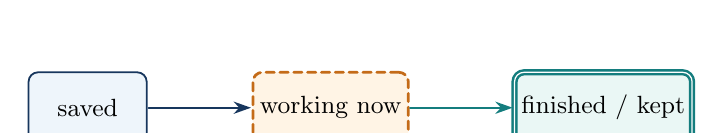
\begin{tikzpicture}[font=\small,>={Stealth[length=2.2mm,width=1.55mm]},node distance=13mm]
  \node[dsnode] (stored) {saved};
  \node[dsnode,active,right=of stored] (current) {working now};
  \node[dsnode,visited,right=of current] (done) {finished / kept};
  \draw[flowarrow] (stored)--(current);
  \draw[flowarrow,teal] (current)--(done);
\end{tikzpicture}
\end{visualbox}

\visualguidesection{Array and \texttt{vector}}
An array is a row of values. Each box has a number called an index. A C++
\texttt{vector} can grow, but we still use indexes in the same way.

\begin{visualbox}{An array is a row of numbered boxes}
\centering
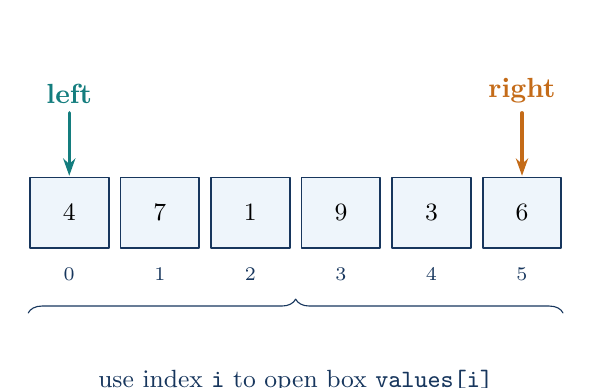
\begin{tikzpicture}[font=\small,>={Stealth[length=2.2mm,width=1.55mm]}]
  \foreach \x/\v in {0/4,1/7,2/1,3/9,4/3,5/6} {
    \node[arraycell] (a\x) at (1.15*\x,0) {\v};
    \node[below=1mm of a\x,font=\scriptsize,text=navy] {\x};
  }
  \node[above=8mm of a0,text=teal,font=\bfseries] (l) {left};
  \node[above=8mm of a5,text=orange,font=\bfseries] (r) {right};
  \draw[->,very thick,teal] (l)--(a0.north);
  \draw[->,very thick,orange] (r)--(a5.north);
  \draw[decorate,decoration={brace,amplitude=5pt},navy]
    ([yshift=-8mm]a0.south west)--([yshift=-8mm]a5.south east)
    node[midway,below=6mm]{use index \texttt{i} to open box \texttt{values[i]}};
\end{tikzpicture}
\end{visualbox}

Arrays appear in two-pointer scans, binary search, bit results, prices, house
values, traversal orders, and one-dimensional dynamic programming.

\visualguidesection{String and reading position}
A string is a row of characters. We keep one position to show where reading
starts and use the length to know where it stops.

\begin{visualbox}{The first number tells us how many letters to read}
\centering
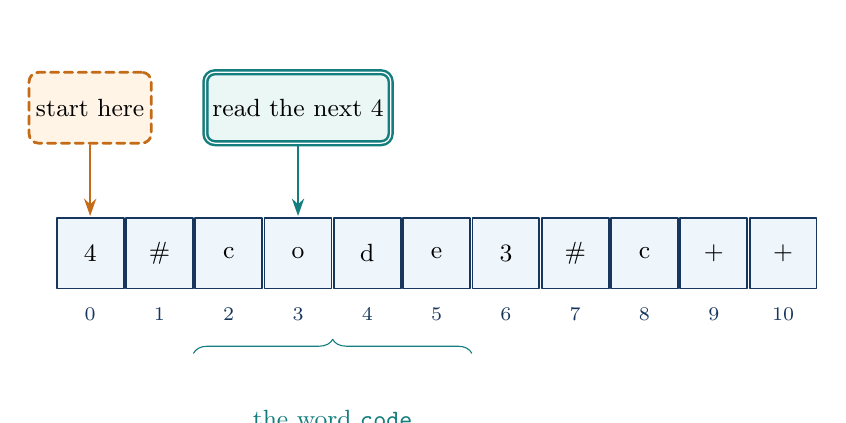
\begin{tikzpicture}[font=\small,>={Stealth[length=2.2mm,width=1.55mm]}]
  \foreach \x/\v in {0/4,1/\#,2/c,3/o,4/d,5/e,6/3,7/\#,8/c,9/+,10/+} {
    \node[arraycell,minimum width=8.5mm] (s\x) at (0.88*\x,0) {\v};
    \node[below=1mm of s\x,font=\scriptsize,text=navy] {\x};
  }
  \node[dsnode,active,above=9mm of s0] (cursor) {start here};
  \draw[flowarrow,orange] (cursor)--(s0.north);
  \node[dsnode,visited,above=9mm of s3] (payload) {read the next 4};
  \draw[flowarrow,teal] (payload)--(s3.north);
  \draw[decorate,decoration={brace,amplitude=5pt},teal]
    ([yshift=-8mm]s2.south west)--([yshift=-8mm]s5.south east)
    node[midway,below=6mm]{the word \texttt{code}};
\end{tikzpicture}

\smallskip
The first number is 4, so we read the next four letters.
\end{visualbox}

\visualguidesection{Remember the best earlier value}
For stock profit, we only need the cheapest price seen before today.

\begin{visualbox}{For each sell day, use the cheapest earlier price}
\centering
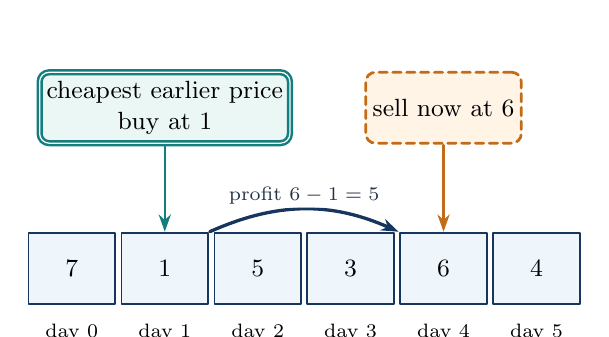
\begin{tikzpicture}[font=\small,>={Stealth[length=2.2mm,width=1.55mm]}]
  \foreach \x/\v in {0/7,1/1,2/5,3/3,4/6,5/4} {
    \node[arraycell,minimum width=11mm] (p\x) at (1.18*\x,0) {\v};
    \node[below=1mm of p\x,font=\scriptsize] {day \x};
  }
  \node[dsnode,visited,above=11mm of p1] (buy) {cheapest earlier price\\buy at 1};
  \node[dsnode,active,above=11mm of p4] (sell) {sell now at 6};
  \draw[flowarrow,teal] (buy)--(p1.north);
  \draw[flowarrow,orange] (sell)--(p4.north);
  \draw[->,very thick,navy] (p1.north east) to[bend left=24]
    node[edgelabel,above]{profit \(6-1=5\)} (p4.north west);
\end{tikzpicture}
\end{visualbox}

\visualguidesection{Hash set and hash map}
A hash set answers ``Have I seen this key?'' A hash map saves extra information
beside the key, such as an index.

\begin{visualbox}{A key is changed into a small bucket number}
\centering
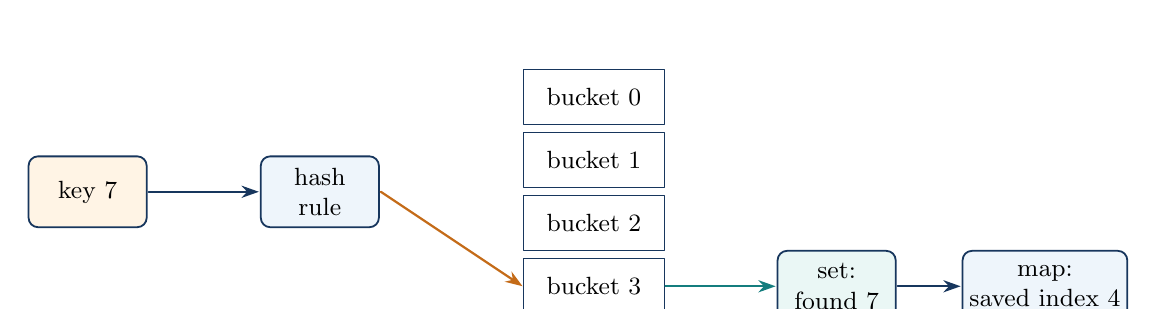
\begin{tikzpicture}[font=\small,>={Stealth[length=2.2mm,width=1.55mm]},node distance=5mm]
  \node[dsnode,fill=softorange] (key) {key 7};
  \node[dsnode,right=14mm of key] (hash) {hash\\rule};
  \draw[flowarrow] (key)--(hash);
  \foreach \y/\label in {0/0,1/1,2/2,3/3} {
    \node[draw=navy,minimum width=18mm,minimum height=7mm,
      right=18mm of hash,yshift={(1.5-\y)*8mm}] (b\y) {bucket \label};
  }
  \draw[flowarrow,orange] (hash.east)--(b3.west);
  \node[dsnode,right=14mm of b3,fill=softteal] (set) {set:\\found 7};
  \node[dsnode,right=8mm of set,fill=softblue] (map) {map:\\saved index 4};
  \draw[flowarrow,teal] (b3)--(set);
  \draw[flowarrow] (set)--(map);
\end{tikzpicture}

\smallskip
A hash table normally finds a saved key quickly. Spreading keys among the
buckets keeps it fast.
\end{visualbox}

\visualguidesection{Stack and function calls}
A stack handles the newest item first. Function calls use a stack too: the
newest call finishes before the older call below it.

\begin{visualbox}{Function calls stack on top of one another}
\centering
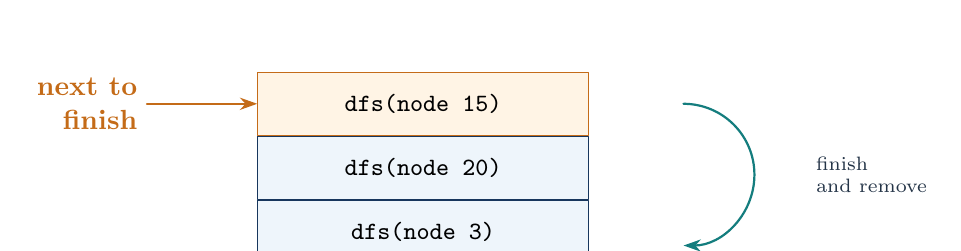
\begin{tikzpicture}[font=\small,>={Stealth[length=2.2mm,width=1.55mm]}]
  \node[draw=navy,fill=softblue,minimum width=42mm,minimum height=8mm] (f0) at (0,0)
    {\texttt{dfs(node 3)}};
  \node[draw=navy,fill=softblue,minimum width=42mm,minimum height=8mm,
    above=0mm of f0] (f1) {\texttt{dfs(node 20)}};
  \node[draw=orange,fill=softorange,minimum width=42mm,minimum height=8mm,
    above=0mm of f1] (f2) {\texttt{dfs(node 15)}};
  \node[left=14mm of f2,text=orange,font=\bfseries,align=right] (top) {next to\\finish};
  \draw[flowarrow,orange] (top)--(f2);
  \draw[->,thick,teal] ([xshift=12mm]f2.east) arc[start angle=90,end angle=-90,radius=9mm]
    node[edgelabel,right=7mm,midway,align=left]{finish\\and remove};
\end{tikzpicture}
\end{visualbox}

The stack grows by one box for each unfinished function call.

\visualguidesection{A problem can split into choices}
This picture shows every choice a function may try. Each choice creates a
smaller version of the same problem.

\begin{visualbox}{One problem splits into smaller choices}
\centering
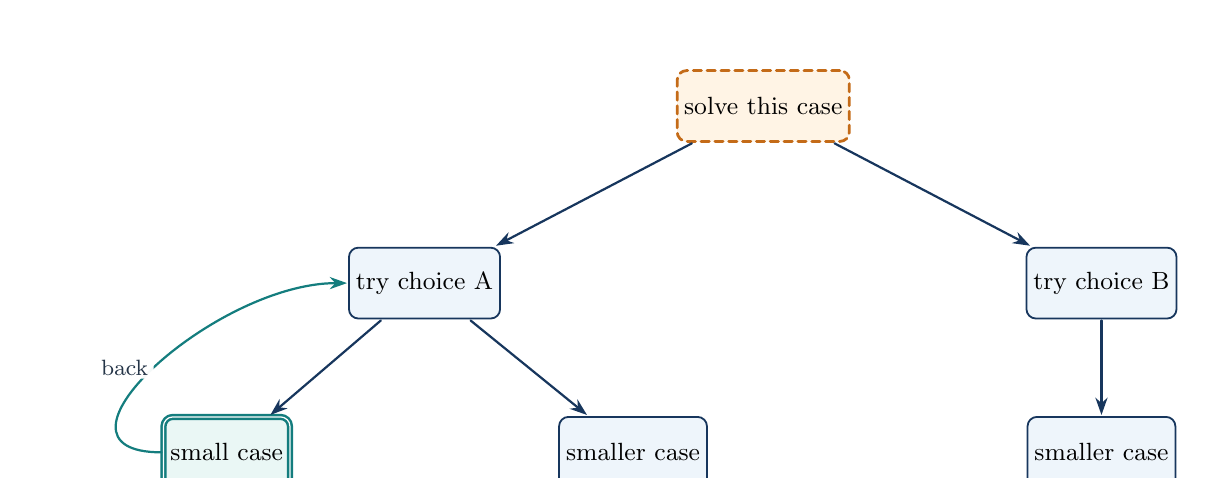
\begin{tikzpicture}[font=\small,>={Stealth[length=2.2mm,width=1.55mm]}]
  \node[dsnode,active] (r) {solve this case};
  \node[dsnode,below left=13mm and 22mm of r] (a) {try choice A};
  \node[dsnode,below right=13mm and 22mm of r] (b) {try choice B};
  \node[dsnode,visited,below left=12mm and 7mm of a] (a1) {small case};
  \node[dsnode,below right=12mm and 7mm of a] (a2) {smaller case};
  \node[dsnode,below=12mm of b] (b1) {smaller case};
  \draw[flowarrow] (r)--(a); \draw[flowarrow] (r)--(b);
  \draw[flowarrow] (a)--(a1); \draw[flowarrow] (a)--(a2);
  \draw[flowarrow] (b)--(b1);
  \draw[flowarrow,teal] (a1.west)
    to[out=180,in=180,looseness=1.35]
    node[edgelabel,left,font=\footnotesize]{back} (a.west);
\end{tikzpicture}
\end{visualbox}

\visualguidesection{Queue}
A queue removes the oldest item first. We remove from the front and add new
items at the back.

\begin{visualbox}{Queue: remove at the front, add at the back}
\centering
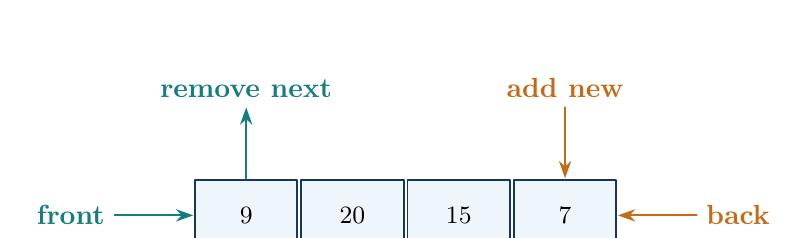
\begin{tikzpicture}[font=\small,>={Stealth[length=2.2mm,width=1.55mm]}]
  \foreach \x/\v in {0/9,1/20,2/15,3/7} {
    \node[arraycell,minimum width=13mm] (q\x) at (1.35*\x,0) {\v};
  }
  \node[left=10mm of q0,text=teal,font=\bfseries] (front) {front};
  \node[right=10mm of q3,text=orange,font=\bfseries] (back) {back};
  \draw[flowarrow,teal] (front)--(q0);
  \draw[flowarrow,orange] (back)--(q3);
  \node[above=9mm of q0,text=teal,font=\bfseries] (pop) {remove next};
  \node[above=9mm of q3,text=orange,font=\bfseries] (push) {add new};
  \draw[flowarrow,teal] (q0.north)--(pop.south);
  \draw[flowarrow,orange] (push.south)--(q3.north);
\end{tikzpicture}
\end{visualbox}

\visualguidesection{Singly linked list}
Each node stores a value and an arrow to the next node. To move through the
list, follow the arrows.

\begin{visualbox}{Each node points to the next node}
\centering
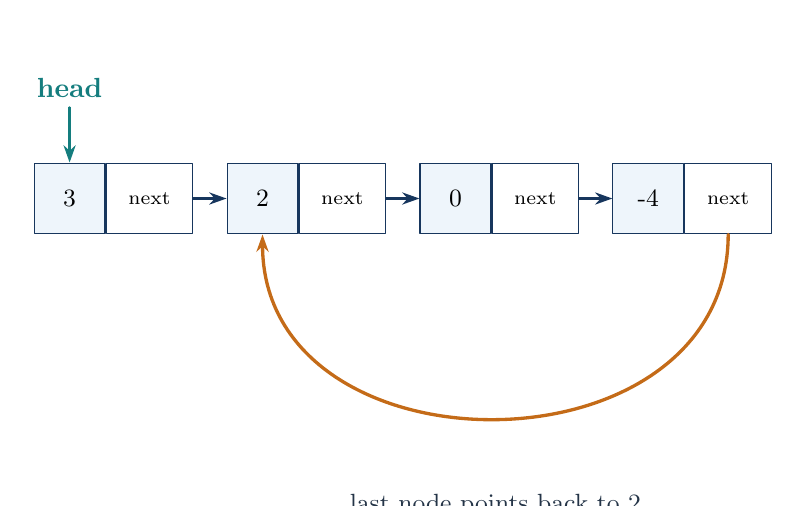
\begin{tikzpicture}[font=\small,>={Stealth[length=2.2mm,width=1.55mm]}]
  \foreach \x/\v in {0/3,1/2,2/0,3/-4} {
    \node[draw=navy,fill=softblue,minimum width=9mm,minimum height=9mm] (v\x)
      at (2.45*\x,0.7) {\v};
    \node[draw=navy,fill=white,minimum width=11mm,minimum height=9mm,
      right=0mm of v\x,font=\scriptsize] (p\x) {next};
  }
  \draw[flowarrow] (p0.east)--(v1.west);
  \draw[flowarrow] (p1.east)--(v2.west);
  \draw[flowarrow] (p2.east)--(v3.west);
  \draw[->,very thick,orange] (p3.south)
    to[out=-90,in=-90,looseness=1.35]
    node[edgelabel,midway,below=9mm,font=\small]{last node points back to 2} (v1.south);
  \node[above=7mm of v0,text=teal,font=\bfseries] (head) {head};
  \draw[flowarrow,teal] (head)--(v0.north);
\end{tikzpicture}
\end{visualbox}

\visualguidesection{Binary tree}
A binary-tree node can point to a left child and a right child. Every node
below one node forms that node's branch.

\begin{visualbox}{A node can have a left and a right child}
\centering
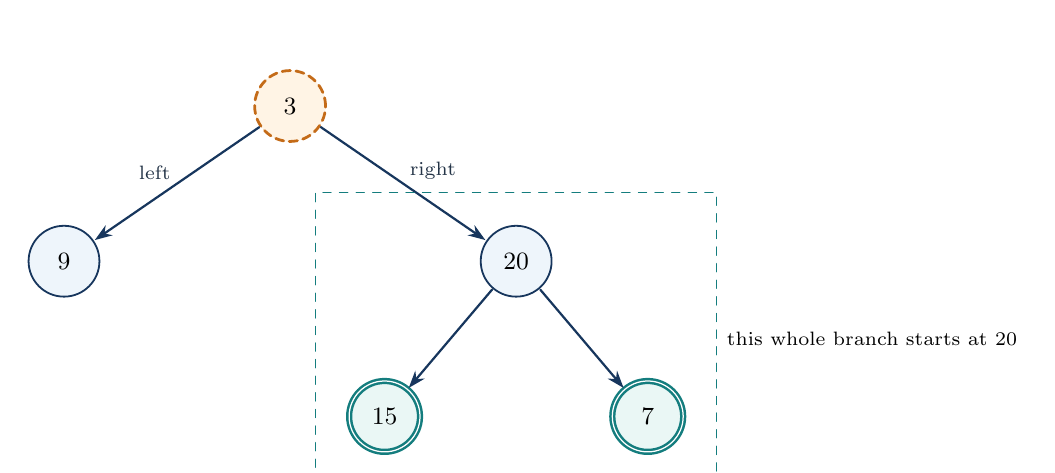
\begin{tikzpicture}[font=\small,>={Stealth[length=2.2mm,width=1.55mm]}]
  \node[trienode,active] (r) {3};
  \node[trienode,below left=13mm and 22mm of r] (l) {9};
  \node[trienode,below right=13mm and 22mm of r] (q) {20};
  \node[trienode,visited,below left=13mm and 10mm of q] (a) {15};
  \node[trienode,visited,below right=13mm and 10mm of q] (b) {7};
  \draw[flowarrow] (r)--node[edgelabel,above left,font=\scriptsize]{left} (l);
  \draw[flowarrow] (r)--node[edgelabel,above right,font=\scriptsize]{right} (q);
  \draw[flowarrow] (q)--(a); \draw[flowarrow] (q)--(b);
  \node[draw=teal,dashed,fit=(q)(a)(b),inner sep=4mm,
    label=right:{\scriptsize this whole branch starts at 20}] {};
\end{tikzpicture}
\end{visualbox}

\visualguidesection{Trie: words that share a beginning}
A Trie stores one letter at a time. Words with the same beginning follow the
same path until their letters become different.

\begin{visualbox}{The words \texttt{app} and \texttt{apple} share one path}
\centering
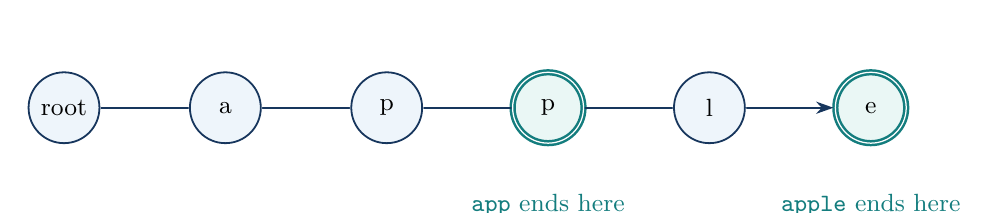
\begin{tikzpicture}[font=\small,>={Stealth[length=2.2mm,width=1.55mm]},node distance=11mm]
  \node[trienode] (r) {root};
  \node[trienode,right=of r] (a) {a};
  \node[trienode,right=of a] (p1) {p};
  \node[trienode,visited,right=of p1] (p2) {p};
  \node[trienode,right=of p2] (l) {l};
  \node[trienode,visited,right=of l] (e) {e};
  \draw[flowarrow] (r)--(a)--(p1)--(p2)--(l)--(e);
  \node[below=5mm of p2,text=teal]{\texttt{app} ends here};
  \node[below=5mm of e,text=teal]{\texttt{apple} ends here};
\end{tikzpicture}
\end{visualbox}

\visualguidesection{Graph and adjacency list}
A graph has numbered points joined by lines. For each point, a neighbor list
records the points directly connected to it.

\begin{visualbox}{The same graph shown as neighbor lists}
\centering
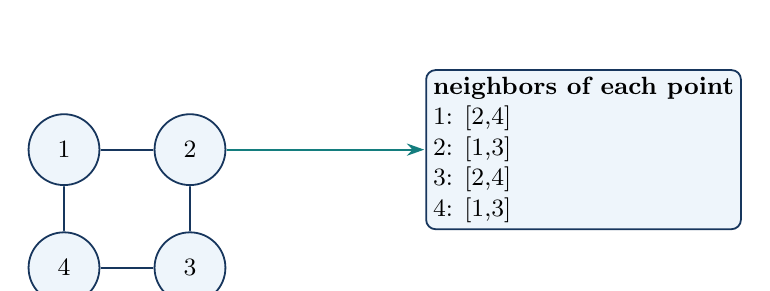
\begin{tikzpicture}[font=\small,>={Stealth[length=2.2mm,width=1.55mm]}]
  \node[trienode] (g1) at (0,1) {1};
  \node[trienode] (g2) at (1.6,1) {2};
  \node[trienode] (g3) at (1.6,-0.5) {3};
  \node[trienode] (g4) at (0,-0.5) {4};
  \draw[-,thick,navy] (g1)--(g2)--(g3)--(g4)--(g1);
  \node[dsnode,align=left,right=25mm of g2] (adj) {
    \textbf{neighbors of each point}\\
    1: [2,4]\\2: [1,3]\\3: [2,4]\\4: [1,3]
  };
  \draw[flowarrow,teal] (g2.east)--(adj.west);
\end{tikzpicture}
\end{visualbox}

\visualguidesection{Heap: quickly see the largest or smallest value}
A max heap keeps the largest value on top. A min heap keeps the smallest value
on top, so that value can be taken next.

\begin{visualbox}{The top shows the next value we can take}
\centering
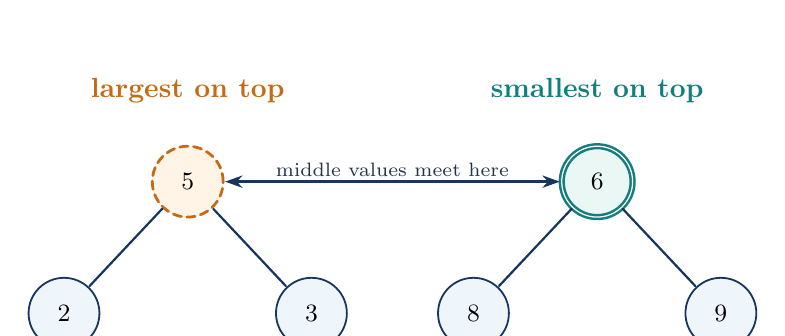
\begin{tikzpicture}[font=\small,>={Stealth[length=2.2mm,width=1.55mm]}]
  \node[trienode,active] (ma) at (0,1.4) {5};
  \node[trienode,below left=10mm and 9mm of ma] (mb) {2};
  \node[trienode,below right=10mm and 9mm of ma] (mc) {3};
  \draw[-,thick,navy] (ma)--(mb); \draw[-,thick,navy] (ma)--(mc);
  \node[above=4mm of ma,text=orange,font=\bfseries]{largest on top};

  \node[trienode,visited] (na) at (5.2,1.4) {6};
  \node[trienode,below left=10mm and 9mm of na] (nb) {8};
  \node[trienode,below right=10mm and 9mm of na] (nc) {9};
  \draw[-,thick,navy] (na)--(nb); \draw[-,thick,navy] (na)--(nc);
  \node[above=4mm of na,text=teal,font=\bfseries]{smallest on top};
  \draw[<->,very thick,navy] (ma.east)--node[edgelabel,above]{middle values meet here} (na.west);
\end{tikzpicture}
\end{visualbox}

\visualguidesection{A table that reuses earlier answers}
A DP array saves answers already found. The colored boxes show which earlier
answers are used for the next box.

\begin{visualbox}{Choose the better of two earlier answers}
\centering
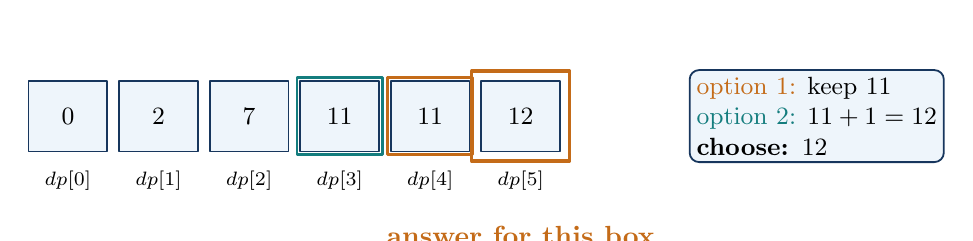
\begin{tikzpicture}[font=\small,>={Stealth[length=2.2mm,width=1.55mm]}]
  \foreach \x/\v in {0/0,1/2,2/7,3/11,4/11,5/12} {
    \node[arraycell] (d\x) at (1.15*\x,0) {\v};
    \node[below=1mm of d\x,font=\scriptsize] {\(dp[\x]\)};
  }
  \node[draw=teal,line width=1pt,fit=(d3),inner sep=0.6pt] {};
  \node[draw=orange,line width=1pt,fit=(d4),inner sep=0.6pt] {};
  \node[draw=orange,very thick,fit=(d5),inner sep=1mm] {};
  \node[dsnode,fill=softblue,right=16mm of d5,align=left] (rule) {
    \textcolor{orange}{option 1: }keep 11\\
    \textcolor{teal}{option 2: }\(11+1=12\)\\
    \textbf{choose: }12};
  \node[below=8mm of d5,text=orange,font=\bfseries] {answer for this box};
\end{tikzpicture}
\end{visualbox}

First decide what each box means. Then fill the boxes only after the earlier
answers they need are ready.

\visualguidesection{Binary-search interval}
Binary search keeps the part that may still contain the answer and throws away
the half that cannot contain it.

\begin{visualbox}{Keep only the half that may contain the answer}
\centering
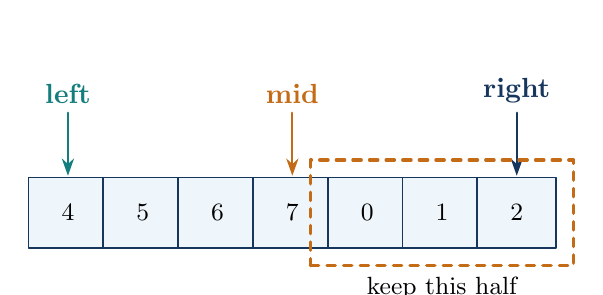
\begin{tikzpicture}[font=\small,>={Stealth[length=2.2mm,width=1.55mm]}]
  \foreach \x/\v in {0/4,1/5,2/6,3/7,4/0,5/1,6/2} {
    \node[arraycell] (b\x) at (0.95*\x,0) {\v};
  }
  \node[above=8mm of b0,text=teal,font=\bfseries] (left) {left};
  \node[above=8mm of b3,text=orange,font=\bfseries] (mid) {mid};
  \node[above=8mm of b6,text=navy,font=\bfseries] (right) {right};
  \draw[flowarrow,teal] (left)--(b0.north);
  \draw[flowarrow,orange] (mid)--(b3.north);
  \draw[flowarrow] (right)--(b6.north);
  \node[draw=orange,very thick,dashed,fit=(b4)(b5)(b6),inner sep=2mm,
    label=below:{keep this half}] {};
\end{tikzpicture}
\end{visualbox}

\visualguidesection{Binary digits and right shift}
A number can be written with only 0s and 1s. Shifting right removes the last
binary digit and leaves a smaller number.

\begin{visualbox}{Shifting right drops the last binary digit}
\centering
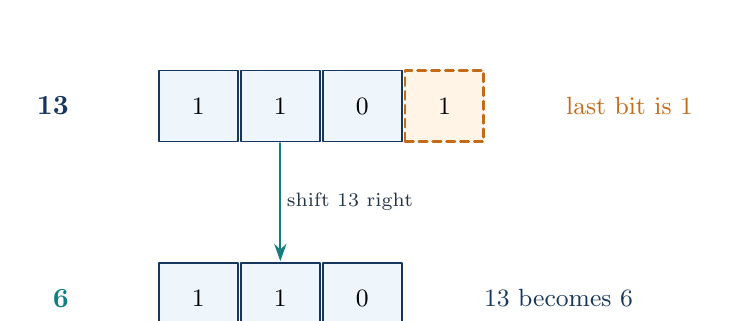
\begin{tikzpicture}[font=\small,>={Stealth[length=2.2mm,width=1.55mm]}]
  \node[arraycell] (x3) at (0,0) {1};
  \node[arraycell,right=0mm of x3] (x2) {1};
  \node[arraycell,right=0mm of x2] (x1) {0};
  \node[arraycell,active,right=0mm of x1] (x0) {1};
  \node[left=10mm of x3,font=\bfseries,text=navy] {13};
  \node[right=9mm of x0,text=orange] {last bit is 1};

  \node[arraycell,below=15mm of x3] (y2) {1};
  \node[arraycell,right=0mm of y2] (y1) {1};
  \node[arraycell,right=0mm of y1] (y0) {0};
  \node[left=10mm of y2,font=\bfseries,text=teal] {6};
  \draw[flowarrow,teal] (x2.south)--node[edgelabel,right]{shift 13 right} (y1.north);
  \node[right=9mm of y0,text=navy] {13 becomes 6};
\end{tikzpicture}
\end{visualbox}

\clearpage


% =================================================
% TWO SUM
% =================================================

\patternintoc{Array Patterns}
\problemstart{Two Sum}{1}{Easy}{Arrays and hashing}{\texttt{unordered\_map}}

\subsection{The Problem}

You receive a sequence of integers and a required total. Find two different
positions whose values combine to that total, then return those positions.
Assume the input has one valid pair.

\subsection{Examples and Rules}

\begin{conceptbox}{Read the output carefully}
The problem returns \emph{indices}, not the two values. Array positions use
zero-based indexing, and the same position cannot be used twice.

\medskip
\begin{center}
\begin{tabular}{@{}lll@{}}
\toprule
Input & Matching values & Output \\
\midrule
\texttt{[4,10,-2,7]}, target \texttt{8} & $10+(-2)=8$ & \texttt{[1,2]} \\
\texttt{[5,1,9]}, target \texttt{14} & $5+9=14$ & \texttt{[0,2]} \\
\texttt{[6,6]}, target \texttt{12} & $6+6=12$ & \texttt{[0,1]} \\
\bottomrule
\end{tabular}
\end{center}
\end{conceptbox}

For a compact dry run, use \texttt{[2,7,11,15]} with target 9. Its indexed
array is
\[
\begin{array}{c|cccc}
\text{Index} & 0 & 1 & 2 & 3 \\ \hline
\text{Value} & 2 & 7 & 11 & 15
\end{array}
\]
Because \(\texttt{nums[0]}+\texttt{nums[1]}=2+7=9\), the answer is
\texttt{[0,1]}.


% =================================================
% BREAKING DOWN THE PROBLEM
% =================================================

\subsection{What We Need to Find}

The input consists of:

\begin{itemize}
    \item An array of integers called \texttt{nums}.
    \item An integer called \texttt{target}.
\end{itemize}

Our goal is to find two elements in the array whose sum is equal
to the target and return their indices.


% =================================================
% DATA STRUCTURE
% =================================================

\subsection{Data Structure: Hash Table}

We can use a \textbf{hash table} to efficiently solve this problem.

In C++, an \texttt{unordered\_map} can be used to implement a hash
table.

The hash table will store values that we have already visited,
along with their matching indices.

The main idea is to calculate the \textbf{complement} of the current
element.

If the current element is \(x\), then the required complement is: \(\text{complement} = \texttt{target} - x\)

This comes from: \(x + \text{complement} = \texttt{target}\)

So: \(\boxed{\text{complement} = \texttt{target} - x}\)

For every element in the array, we check whether this complement
already exists in our hash table.


% =================================================
% HOW THE HASH TABLE WORKS
% =================================================

\subsection{How the Hash Table Works}

While iterating through the array, we store every element that
we have already visited in the hash table.

For the current element, we calculate: \(\text{complement} = \texttt{target} - \text{current element}\)

We then check whether the complement exists in the hash table.

\begin{itemize}
    \item If the complement exists, we have found the required pair.
    \item If the complement does not exist, we store the current
    element and its index in the hash table.
\end{itemize}

This lets us find the required pair in a single traversal
of the array.

\begin{visualbox}{Two Sum: save a number, then find the one needed}
\centering
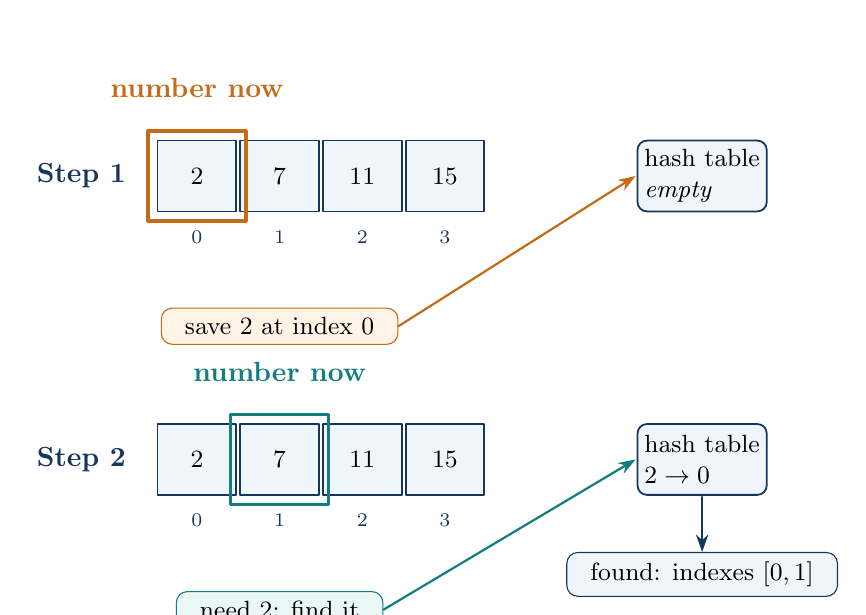
\begin{tikzpicture}[>={Stealth[length=2.2mm,width=1.55mm]},font=\small]
  % Keep the step labels in their own left margin, clear of the first cell.
  \node[anchor=east,text=navy,font=\bfseries] at (-0.78,1.8) {Step 1};
  \foreach \x/\value in {0/2,1/7,2/11,3/15} {
    \node[arraycell] (a\x) at (1.05*\x,1.8) {\value};
    \node[below=1mm of a\x,font=\scriptsize,text=navy] {\x};
  }
  \node[draw=orange,very thick,fit=(a0),inner sep=1mm] {};
  \node[above=4mm of a0,text=orange,font=\bfseries] {number now};
  \node[dsnode,align=left,right=19mm of a3] (empty)
    {hash table\\\textit{empty}};
  \node[below=12mm of a1,draw=orange,fill=softorange,rounded corners,
    inner xsep=3mm,inner ysep=1.2mm] (store) {save 2 at index 0};
  \draw[flowarrow,orange] (store.east) -- (empty.west);

  \node[anchor=east,text=navy,font=\bfseries] at (-0.78,-1.8) {Step 2};
  \foreach \x/\value in {0/2,1/7,2/11,3/15} {
    \node[arraycell] (b\x) at (1.05*\x,-1.8) {\value};
    \node[below=1mm of b\x,font=\scriptsize,text=navy] {\x};
  }
  \node[draw=teal,very thick,fit=(b1),inner sep=1mm] {};
  \node[above=4mm of b1,text=teal,font=\bfseries] {number now};
  \node[dsnode,align=left,right=19mm of b3] (filled)
    {hash table\\$2\to0$};
  \node[below=12mm of b1,draw=teal,fill=softteal,rounded corners,
    inner xsep=3mm,inner ysep=1.2mm] (look) {need 2: find it};
  \draw[flowarrow,teal] (look.east) -- (filled.west);
  \node[below=7mm of filled,draw=navy,fill=softblue,rounded corners,
    inner xsep=3mm,inner ysep=1.2mm] (answer) {found: indexes $[0,1]$};
  \draw[flowarrow] (filled) -- (answer);
\end{tikzpicture}

\smallskip
Before checking a number, the table contains only numbers seen earlier.
\end{visualbox}

\begin{invariantbox}{the table contains only earlier numbers}
Before index \(i\) is processed, every entry in the hash map came from an
index smaller than \(i\). A successful complement lookup uses two
different positions and automatically keeps the scan order.
\end{invariantbox}

The two rows above are the full dry run. The first value is remembered. At
the next index, the needed value is already in the table, so the answer is
found without scanning the earlier part of the array again.


% =================================================
% PSEUDOCODE
% =================================================

\subsection{Pseudocode}

The overall pseudocode is:

\begin{enumerate}
    \item Start an empty hash table to store previously seen values and their
    indices.

    \item Loop over every element in the array.

    \item For the current element, calculate its complement:
    \(\text{complement} = \texttt{target} - \text{current element}\)

    \item Check whether the complement exists in the hash table.

    \item If the complement exists:
    \begin{itemize}
        \item Return the index of the complement from the hash table.
        \item Return the index of the current element.
    \end{itemize}

    \item If the complement does not exist:
    \begin{itemize}
        \item Insert the current element and its index into the
        hash table.
    \end{itemize}

    \item If no pair is found, return an empty array as an edge case.
\end{enumerate}


% =================================================
% C++ IMPLEMENTATION
% =================================================

\subsection{C++ Implementation}

The hash table can be implemented using
\texttt{unordered\_map} in C++.

\begin{lstlisting}[style=compactcode,caption={Complete C++ solution: Two Sum}]
#include <unordered_map>
#include <vector>

using namespace std;

class Solution {
public:
    vector<int> twoSum(vector<int>& nums, int target) {
        unordered_map<int, int> hashTable;

        for (int i = 0; i < static_cast<int>(nums.size()); ++i) {
            const int complement = target - nums[i];

            if (hashTable.count(complement)) {
                return {hashTable[complement], i};
            }

            hashTable[nums[i]] = i;
        }

        return {};
    }
};
\end{lstlisting}


% =================================================
% STEP-BY-STEP CODE EXPLANATION
% =================================================

\subsection{Code Walkthrough}

\subsubsection{Step 1: Start the Hash Table}

We first create an empty hash table:

\begin{lstlisting}
unordered_map<int, int> hashTable;
\end{lstlisting}

The key represents the value from the array, while the value
stored in the hash table represents its index.

For example: \(\texttt{hashTable[2] = 0}\)

means that the value \(2\) was found at index \(0\).

\subsubsection{Step 2: Traverse the Array}

We iterate through the array:

\begin{lstlisting}
for (int i = 0; i < nums.size(); i++)
\end{lstlisting}

Each element is processed exactly once.

\subsubsection{Step 3: Calculate the Complement}

For the current element \texttt{nums[i]}, calculate:

\begin{lstlisting}
int complement = target - nums[i];
\end{lstlisting}

For example, if: \(\texttt{target}=9\)

and: \(\texttt{nums[i]}=2\)

then: \(\text{complement}=9-2=7\)

So, we need to determine whether \(7\) has already
appeared in the array.

\subsubsection{Step 4: Check the Hash Table}

We check whether the complement exists:

\begin{lstlisting}
if (hashTable.count(complement))
\end{lstlisting}

If it exists, we have found the required pair.

We can then return:

\begin{lstlisting}
return {hashTable[complement], i};
\end{lstlisting}

The hash table provides the index of the previously visited
element, while \(i\) is the index of the current element.

\subsubsection{Step 5: Store the Current Element}

If the complement does not exist, we store the current element
and its index:

\begin{lstlisting}
hashTable[nums[i]] = i;
\end{lstlisting}

This allows future elements to check whether the current element
is their required complement.


% =================================================
% EDGE CASE
% =================================================

\subsection{Edge Case}

If no valid pair is found, we return an empty array:

\begin{lstlisting}
return {};
\end{lstlisting}

This handles the case where there are no elements that satisfy
the required condition.


% =================================================
% TIME AND SPACE COMPLEXITY
% =================================================

\subsection{Time and Space}

\subsubsection{Time Complexity}

The algorithm iterates through the array only once.

So, the time complexity is: \(\boxed{\Oof{n}}\)

where \(n\) is the number of elements in the input array.

The hash table allows us to check whether a complement exists in
constant average time.

\subsubsection{Space Complexity}

In the worst case, we may need to store every element of the
array in the hash table.

So, the space complexity is: \(\boxed{\Oof{n}}\)

So, the overall complexity is: \(\boxed{\text{Time} = O(n)}\) \(\boxed{\text{Space} = O(n)}\)


\chaptercheckpoint
  {A current value needs a previously seen complement.}
  {A value-to-index hash map for the processed prefix.}
  {Inserting before checking and accidentally reusing the same index.}
  {$O(n)$ average time and $O(n)$ space.}

% =================================================
% 3SUM
% =================================================

\problemstart{3Sum}{15}{Medium}{Sorting and two pointers}{Sorted array}

\subsection{The Problem}

Find every distinct group of three values whose sum is zero. Each group must
use three different array positions, and the returned collection must not
repeat the same value triplet.

\subsection{Example}

Consider: \(\texttt{nums}=[-1,0,1,2,-1,-4]\)

The valid triplets are: \([-1,-1,2]\)

and \([-1,0,1]\)

Both triplets have a sum of zero: \(-1+(-1)+2=0\)

and \(-1+0+1=0\)

So, the output is: \([[-1,-1,2],[-1,0,1]]\)

Another example is: \(\texttt{nums}=[0,1,1]\)

There is no combination of three distinct indices whose values
sum to zero, so the result is an empty list.

\subsection{What We Need to Find}

The input is an array of integers called \texttt{nums}.

We need to return all triplets satisfying: \(\texttt{nums[i]}+\texttt{nums[j]}+\texttt{nums[k]}=0\)

where all three indices are different.

We must also make sure that duplicate triplets are not included in
the result.

\subsection{Algorithmic Technique: Two Pointers}

The technique used for this problem is the
\textbf{two-pointer technique}.

The general idea is:

\begin{enumerate}
    \item Sort the input array.
    \item Traverse the array from the beginning.
    \item For each element, use two pointers to search for the
    remaining two elements.
\end{enumerate}

For a fixed element \texttt{nums[i]}, we need to find two values
whose sum is: \(-\texttt{nums[i]}\)

The two pointers are:

\begin{itemize}
    \item \texttt{j}: starts immediately after \texttt{i}.
    \item \texttt{k}: starts at the end of the array.
\end{itemize}

We then calculate: \(\texttt{sum} = \texttt{nums[i]}+\texttt{nums[j]}+\texttt{nums[k]}\)

Because the array is sorted, we can move the pointers intelligently.

\subsection{Pointer Movement}

If: \(\texttt{sum}<0\)

then the sum is too small, so we increment \texttt{j}: \(\texttt{j++}\)

This moves toward a larger value.

If: \(\texttt{sum}>0\)

then the sum is too large, so we decrement \texttt{k}: \(\texttt{k--}\)

This moves toward a smaller value.

If: \(\texttt{sum}=0\)

then we have found a valid triplet.

We add it to the result and move both pointers.

\begin{visualbox}{Pick one number, then move left and right}
\centering
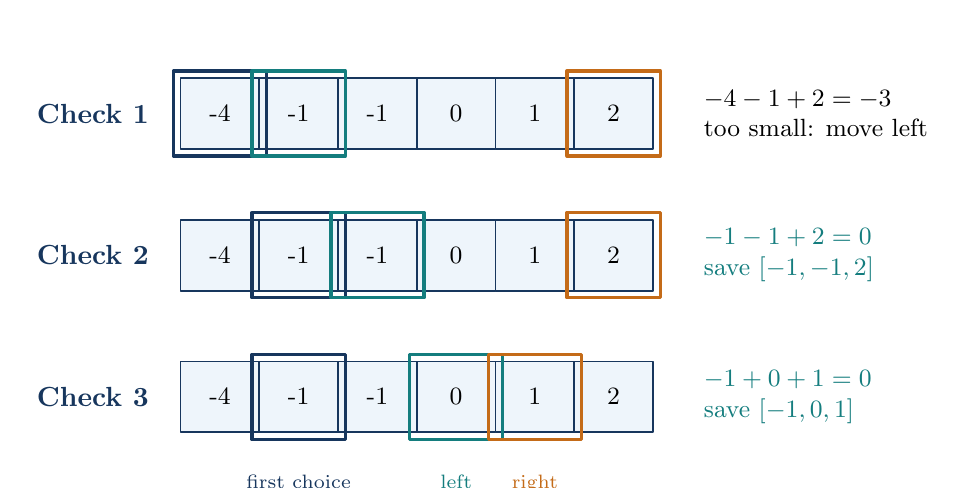
\begin{tikzpicture}[>={Stealth[length=2.2mm,width=1.55mm]},font=\small]
  \foreach \row/\yy in {A/1.8,B/0,C/-1.8} {
    \foreach \x/\value in {0/-4,1/-1,2/-1,3/0,4/1,5/2}
      \node[arraycell] (\row\x) at (1.0*\x,\yy) {\value};
  }
  % Reserve a clear label column instead of letting labels touch the arrays.
  \node[anchor=east,font=\bfseries,text=navy] at (-0.78,1.8) {Check 1};
  \node[draw=navy,very thick,fit=(A0),inner sep=.7mm] {};
  \node[draw=teal,very thick,fit=(A1),inner sep=.7mm] {};
  \node[draw=orange,very thick,fit=(A5),inner sep=.7mm] {};
  \node[right=5mm of A5,align=left] {$-4-1+2=-3$\\too small: move left};

  \node[anchor=east,font=\bfseries,text=navy] at (-0.78,0) {Check 2};
  \node[draw=navy,very thick,fit=(B1),inner sep=.7mm] {};
  \node[draw=teal,very thick,fit=(B2),inner sep=.7mm] {};
  \node[draw=orange,very thick,fit=(B5),inner sep=.7mm] {};
  \node[right=5mm of B5,align=left,text=teal] {$-1-1+2=0$\\save $[-1,-1,2]$};

  \node[anchor=east,font=\bfseries,text=navy] at (-0.78,-1.8) {Check 3};
  \node[draw=navy,very thick,fit=(C1),inner sep=.7mm] {};
  \node[draw=teal,very thick,fit=(C3),inner sep=.7mm] {};
  \node[draw=orange,very thick,fit=(C4),inner sep=.7mm] {};
  \node[right=5mm of C5,align=left,text=teal] {$-1+0+1=0$\\save $[-1,0,1]$};

  \node[below=4mm of C1,text=navy,font=\scriptsize] {first choice};
  \node[below=4mm of C3,text=teal,font=\scriptsize] {left};
  \node[below=4mm of C4,text=orange,font=\scriptsize] {right};
\end{tikzpicture}

\smallskip
If the sum is too small, move left to a larger number. If it is too large,
move right to a smaller number.
\end{visualbox}

\begin{invariantbox}{every pair still worth checking lies between left and right}
After choosing the first number, the remaining possible pairs lie between the
left and right positions. A small sum moves left; a large sum moves right.
\end{invariantbox}

The three array rows show the important pointer changes. Blue marks the fixed
value, teal marks the left pointer, and orange marks the right pointer.

\subsection{Pseudocode}

The overall process is:

\begin{enumerate}
    \item Start an empty result vector.

    \item If the size of \texttt{nums} is less than \(3\), return
    the empty result.

    \item Sort the input array.

    \item Traverse the array using index \texttt{i}.

    \item Skip duplicate values for \texttt{i}.

    \item Set:
    \(\texttt{j}=i+1\)
    and
    \(\texttt{k}=n-1\)

    \item While:
    \(\texttt{j}<\texttt{k}\)
    calculate:
    \(\texttt{sum} = \texttt{nums[i]}+ \texttt{nums[j]}+ \texttt{nums[k]}\)

    \item If the sum is zero:
    \begin{itemize}
        \item Add the triplet to the result.
        \item Skip duplicate values for \texttt{j}.
        \item Skip duplicate values for \texttt{k}.
        \item Increment \texttt{j}.
        \item Decrement \texttt{k}.
    \end{itemize}

    \item Else if the sum is less than zero:
    \(\texttt{j++}\)

    \item Otherwise:
    \(\texttt{k--}\)

    \item Return the result.
\end{enumerate}

\subsection{C++ Implementation}

\begin{lstlisting}[style=compactcode,caption={Complete C++ solution: 3Sum}]
#include <algorithm>
#include <vector>

using namespace std;

class Solution {
public:
    vector<vector<int>> threeSum(vector<int>& nums) {
        vector<vector<int>> result;
        if (nums.size() < 3) return result;
        sort(nums.begin(), nums.end());
        const int n = static_cast<int>(nums.size());
        for (int i = 0; i < n - 2; ++i) {
            if (i > 0 && nums[i] == nums[i - 1]) continue;
            int j = i + 1;
            int k = n - 1;
            while (j < k) {
                const long long sum =
                    static_cast<long long>(nums[i]) + nums[j] + nums[k];
                if (sum == 0) {
                    result.push_back({nums[i], nums[j], nums[k]});
                    while (j < k && nums[j] == nums[j + 1]) ++j;
                    while (j < k && nums[k] == nums[k - 1]) --k;
                    ++j;
                    --k;
                } else if (sum < 0) {
                    ++j;
                } else {
                    --k;
                }
            }
        }
        return result;
    }
};
\end{lstlisting}

\subsection{Code Walkthrough}

\subsubsection{Step 1: Start the Result}

We first create a vector to store all valid triplets:

\begin{lstlisting}
vector<vector<int>> result;
\end{lstlisting}

If there are fewer than three elements, a triplet cannot be
formed:

\begin{lstlisting}
if (nums.size() < 3) {
    return result;
}
\end{lstlisting}

\subsubsection{Step 2: Sort the Array}

We sort the array:

\begin{lstlisting}
sort(nums.begin(), nums.end());
\end{lstlisting}

Sorting is important because it allows the two-pointer technique
to determine which pointer should move based on the current sum.

For example: \([0,-1,2,-1,-4,1]\)

becomes: \([-4,-1,-1,0,1,2]\)

\subsubsection{Step 3: Fix the First Element}

We traverse the array:

\begin{lstlisting}
for (int i = 0; i < nums.size() - 2; i++)
\end{lstlisting}

The index \texttt{i} represents the first element of the triplet.

For every fixed \texttt{i}, we search for two additional values.

\subsubsection{Handling Duplicate Values for \texttt{i}}

Since duplicate triplets are not allowed, we skip duplicate values:

\begin{lstlisting}
if (i > 0 && nums[i] == nums[i - 1]) {
    continue;
}
\end{lstlisting}

This prevents us from processing the same first value multiple
times.

\subsubsection{Step 4: Start the Two Pointers}

For every fixed \texttt{i}, we start:

\begin{lstlisting}
int j = i + 1;
int k = nums.size() - 1;
\end{lstlisting}

So: \(i < j < k\)

The pointer \texttt{j} starts immediately after \texttt{i},
while \texttt{k} starts at the last element.

\subsubsection{Step 5: Calculate the Sum}

While: \(\texttt{j}<\texttt{k}\)

we calculate:

\begin{lstlisting}
int sum = nums[i] + nums[j] + nums[k];
\end{lstlisting}

There are three possibilities.

\subsubsection{Case 1: Sum Equals Zero}

If: \(\texttt{sum}=0\)

we have found a valid triplet.

We add it to the result:

\begin{lstlisting}
result.push_back({
    nums[i],
    nums[j],
    nums[k]
});
\end{lstlisting}

We then skip duplicate values for both pointers and move them
toward each other.

\subsubsection{Case 2: Sum Is Less Than Zero}

If: \(\texttt{sum}<0\)

we need to increase the sum.

Because the array is sorted, we move \texttt{j} to the right:

\begin{lstlisting}
j++;
\end{lstlisting}

This gives us a potentially larger value.

\subsubsection{Case 3: Sum Is Greater Than Zero}

If: \(\texttt{sum}>0\)

we need to decrease the sum.

Because the array is sorted, we move \texttt{k} to the left:

\begin{lstlisting}
k--;
\end{lstlisting}

This gives us a potentially smaller value.

\subsection{Why Sorting Helps}

Sorting creates an important property: \(\texttt{nums[j]} \leq \texttt{nums[k]}\)

So, if the current sum is too small, moving \texttt{j}
forward increases the sum.

If the current sum is too large, moving \texttt{k} backward
decreases the sum.

This lets us search for the required pair efficiently without
checking every possible pair.

\subsection{Handling Duplicates}

Duplicate triplets are not allowed.

After finding a valid triplet, we skip duplicate values for
\texttt{j}:

\begin{lstlisting}
while (j < k && nums[j] == nums[j + 1]) {
    j++;
}
\end{lstlisting}

Similarly, we skip duplicate values for \texttt{k}:

\begin{lstlisting}
while (j < k && nums[k] == nums[k - 1]) {
    k--;
}
\end{lstlisting}

After that, both pointers are moved:

\begin{lstlisting}
j++;
k--;
\end{lstlisting}


% =================================================
% COMPLEXITY
% =================================================

\subsection{Time and Space}

The array is first sorted, which takes: \(O(n\log n)\)

After sorting, we use a loop over the array and a two-pointer
scan for each fixed element.

The resulting dominant complexity is: \(\boxed{O(n^2)}\)

where \(n\) is the number of elements in the input array.

The sorting step is smaller than the \(O(n^2)\) two-pointer
processing for the overall asymptotic complexity.

The extra space depends on the sorting implementation. The
two-pointer portion itself uses constant extra space, aside
from the space required for the returned result. The overall time complexity
is \(O(n^2)\), and the two-pointer scan uses \(O(1)\) extra space, excluding
the output vector and implementation-dependent sorting stack space.

\subsection{3Sum Summary}

The key idea is:

\begin{enumerate}
    \item Sort the array.
    \item Fix one element.
    \item Use two pointers to find the remaining two elements.
    \item If the sum is too small, move the left pointer right.
    \item If the sum is too large, move the right pointer left.
    \item If the sum is zero, record the triplet.
    \item Skip duplicates to ensure unique triplets.
\end{enumerate}

So, the two-pointer technique reduces the problem to an
efficient \(O(n^2)\) solution.

\chaptercheckpoint
  {A sorted array asks for unique tuples satisfying a target sum.}
  {One fixed index, two moving pointers, and duplicate skipping.}
  {Recording duplicate triplets or moving the wrong pointer after comparing the sum.}
  {$O(n^2)$ time and constant pointer space excluding sorting/output.}

% =================================================
% BEST TIME TO BUY AND SELL STOCK
% =================================================

\problemstart{Best Time to Buy and Sell Stock}{121}{Easy}{Greedy running minimum}{Array}

\subsection{The Problem}

The array \texttt{prices} stores the stock price for each day. Choose one day
to buy and a later day to sell. Return the greatest possible profit. If every
possible transaction loses money, return zero.

\begin{conceptbox}{The ordering rule}
\centering
\textbf{Buy before sell}

\smallskip
For a buy price \(B\) and a later selling price \(S\), \(\text{profit}=S-B.\)
The algorithm may not use a low price that appears after the selling day.
\end{conceptbox}

\subsection{Examples and Rules}

\begin{center}
\begin{tabular}{@{}lll@{}}
\toprule
Prices & Best transaction & Answer \\
\midrule
\texttt{[7,1,5,3,6,4]} & buy at \(1\), sell at \(6\) & \(5\) \\
\texttt{[7,6,4,3,1]} & no profitable sale & \(0\) \\
\bottomrule
\end{tabular}
\end{center}

The first example earns \(6-1=5\). In the decreasing example, every future
price is smaller than its earlier prices, so the best legal answer is zero.

\subsection{First Idea: Try Every Transaction}

The direct method chooses every pair of days \((i,j)\) with \(i<j\), computes
\(\texttt{prices[j]}-\texttt{prices[i]}\), and keeps the largest result.
There are about \(n(n-1)/2\) legal pairs, so this approach takes
\(O(n^2)\) time.

The repeated work is the clue: for every selling day, the brute-force method
searches the earlier days again to find the cheapest possible purchase.

\subsection{Greedy Observation}

For a fixed selling day, the best buying day is always the cheapest earlier
day. So, while scanning from left to right, we only need to remember
the minimum price seen so far.
\[
\boxed{\begin{gathered}
\text{minimum previous price}\longrightarrow\text{current selling price}\\
\longrightarrow\text{best profit}
\end{gathered}}
\]

\begin{visualbox}{For each selling day, keep the cheapest earlier price}
\centering
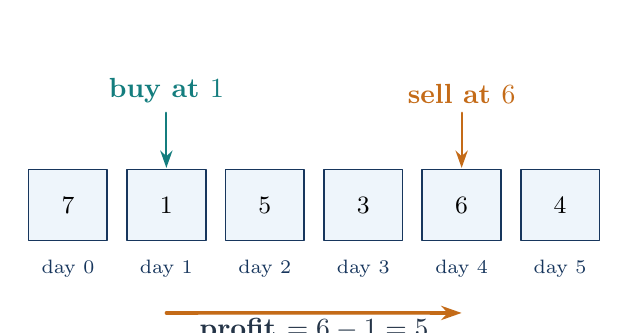
\begin{tikzpicture}[>={Stealth[length=2.2mm,width=1.55mm]},font=\small]
  \foreach \x/\value in {0/7,1/1,2/5,3/3,4/6,5/4} {
    \node[arraycell] (p\x) at (1.25*\x,0) {\value};
    \node[below=1mm of p\x,font=\scriptsize,text=navy] {day \x};
  }
  \node[above=7mm of p1,text=teal,font=\bfseries] (buy) {buy at \(1\)};
  \draw[flowarrow,teal] (buy.south)--(p1.north);
  \node[above=7mm of p4,text=orange,font=\bfseries] (sell) {sell at \(6\)};
  \draw[flowarrow,orange] (sell.south)--(p4.north);
  \draw[-{Stealth[length=2.6mm,width=1.8mm]},very thick,orange]
    ([yshift=-9mm]p1.south) -- node[edgelabel,below,font=\bfseries]{profit \(=6-1=5\)}
    ([yshift=-9mm]p4.south);
\end{tikzpicture}

\smallskip
When day 4 is the selling day, \(1\) is the cheapest price in days 0 through 3.
No other earlier buying price can produce a larger profit that day.
\end{visualbox}

\subsection{The Two Variables}

\begin{conceptbox}{State keeped during the scan}
\begin{tabularx}{\linewidth}{@{}>{\bfseries}p{3cm}X@{}}
\texttt{minPrice} & Smallest price seen up to the current day. Start at positive infinity.\\[2mm]
\texttt{maxProfit} & Greatest legal profit found so far. Start at zero so a loss is never returned.
\end{tabularx}
\end{conceptbox}

\begin{invariantbox}{the two variables summarize the entire processed prefix}
Before moving to the next day, \texttt{minPrice} is the cheapest price in the
processed prefix, and \texttt{maxProfit} is the best legal transaction
entirely inside that prefix. No older price needs to be stored separately.
\end{invariantbox}

\subsection{Step-by-Step Algorithm}

For every price, perform three operations in this order:

\begin{enumerate}
  \item Update the cheapest price:
  \(\texttt{minPrice}=\min(\texttt{minPrice},\texttt{price}).\)
  \item Calculate the profit obtained by selling today:
  \(\texttt{currentProfit}=\texttt{price}-\texttt{minPrice}.\)
  \item Update the best result:
  \(\texttt{maxProfit}=\max(\texttt{maxProfit},\texttt{currentProfit}).\)
\end{enumerate}

Updating \texttt{minPrice} first allows the current day to act as both the new
minimum and a zero-profit sale. This never creates an invalid positive
transaction, and future days may use that price as their buying day.

\subsection{Detailed Visual Dry Run}

\begin{dryrunbox}{Scanning \texttt{[7,1,5,3,6,4]}}
\begin{center}
\begin{tabular}{@{}ccccc@{}}
\toprule
Day & Price & \texttt{minPrice} & Sell-today profit & \texttt{maxProfit} \\
\midrule
0 & 7 & 7 & 0 & 0 \\
1 & 1 & 1 & 0 & 0 \\
2 & 5 & 1 & 4 & 4 \\
3 & 3 & 1 & 2 & 4 \\
4 & 6 & 1 & 5 & 5 \\
5 & 4 & 1 & 3 & 5 \\
\bottomrule
\end{tabular}
\end{center}
\end{dryrunbox}

The minimum changes only when a cheaper buying opportunity appears. The
maximum profit changes only when today's selling price improves the answer.

\subsection{Why the Greedy Choice Is Correct}

Suppose the current selling price is \(P\). For any legal earlier buying price
\(B\), the profit is \(P-B\). With \(P\) fixed, this expression is largest
when \(B\) is as small as possible. So, the cheapest earlier price is
the only buying choice needed for the current day.

Every day is considered once as a possible selling day. As a result, every
best transaction is considered when its selling day is processed, and the
global maximum is correct.

\subsection{Pseudocode}

\begin{lstlisting}[style=pseudocode]
maxProfit(prices):
    minPrice = positive infinity
    bestProfit = 0

    for each price in prices:
        minPrice = min(minPrice, price)
        profitToday = price - minPrice
        bestProfit = max(bestProfit, profitToday)

    return bestProfit
\end{lstlisting}

\subsection{C++ Implementation}

\begin{lstlisting}[style=compactcode,caption={Complete C++ solution: Best Time to Buy and Sell Stock}]
#include <algorithm>
#include <limits>
#include <vector>

using namespace std;

class Solution {
public:
    int maxProfit(vector<int>& prices) {
        int minPrice = numeric_limits<int>::max();
        int maxProfitSeen = 0;

        for (const int price : prices) {
            minPrice = min(minPrice, price);
            const int currentProfit = price - minPrice;
            maxProfitSeen = max(maxProfitSeen, currentProfit);
        }

        return maxProfitSeen;
    }
};
\end{lstlisting}

\begin{conceptbox}{Output and local testing}
This class does not print output by itself. The online judge creates the input, calls
\texttt{maxProfit}, and checks the returned integer. A separate local test
harness was used to compile and validate the method.
\end{conceptbox}

\subsection{Compact Interview Version}

The same update can be written directly with \texttt{std::min} and
\texttt{std::max}. The part to remember is the key rule, not the
number of lines:

\begin{lstlisting}
for (const int price : prices) {
    minPrice = min(minPrice, price);
    maxProfitSeen = max(maxProfitSeen, price - minPrice);
}
\end{lstlisting}

\subsection{Time and Space}

Let \(n\) be the number of days. The loop visits every price exactly once, so
the time complexity is \(O(n)\). Only two running values are stored, so the
extra space is \(O(1)\).

\begin{conceptbox}{Why the extra space is constant}
The implementation stores only a constant number of integers regardless of
the input length. So, its extra-space complexity is \(O(1)\).
\end{conceptbox}

\subsection{Edge Cases and Common Mistakes}

\begin{itemize}
  \item An empty array returns zero because the loop performs no update.
  \item One price cannot form a transaction, so the answer remains zero.
  \item A decreasing array must return zero, not the smallest negative loss.
  \item Update the running minimum using only the current and earlier days.
  \item Do not solve the multiple-transaction variation; this problem allows one transaction.
  \item Do not sort the prices. Sorting destroys the original day order.
\end{itemize}

\subsection{How to Explain It in an Interview}

\begin{revisionbox}{How to explain it in an interview}
I would first mention the \(O(n^2)\) pair check. It repeatedly searches for a
buying price before each sale. During one left-to-right pass, I instead keep
the cheapest price seen so far. For each current price, I calculate the profit
from selling today and update the global maximum. The key rule is that the
minimum and best profit are correct for the processed prefix. Each element is
visited once, so the algorithm takes \(O(n)\) time and \(O(1)\) extra space.
\end{revisionbox}

Useful clarifying questions include whether only one transaction is allowed,
whether buying and selling must occur on different days, and whether returning
zero is required when no profit exists.

\subsection{Pattern-Recognition Clue}

Consider this greedy pattern when each current value should be combined with
the best earlier value:

\[
\boxed{
\begin{gathered}
\text{remember the best earlier value}
\;\rightarrow\;
\text{use today's value}\\[1mm]
\Downarrow\\[-1mm]
\text{update the best answer}
\end{gathered}
}
\]

\subsection{Revision Summary}

\begin{revisionbox}{Best Time to Buy and Sell Stock}
\begin{tabularx}{\linewidth}{@{}>{\bfseries}p{2.7cm}X@{}}
Technique & Greedy running minimum \\
Keep & \texttt{minPrice} and \texttt{maxProfitSeen} \\
Update & Compare today's price with the minimum, then test selling today \\
Complexity & \(O(n)\) time and \(O(1)\) extra space
\end{tabularx}
\end{revisionbox}

\chaptercheckpoint
  {Each current price should be combined with the best earlier buying price.}
  {\texttt{minPrice} and the maximum profit found so far.}
  {Sorting prices or allowing the selling day to precede the buying day.}
  {$O(n)$ time and $O(1)$ extra space.}

% =================================================
% DESIGN ADD AND SEARCH WORDS DATA STRUCTURE
% =================================================

\patternintoc{Trie Patterns}
\problemstart{Design Add and Search Words Data Structure}{211}{Medium}{Trie and recursive DFS}{Trie}

\subsection{Problem Overview}

The goal of this problem is to design a data structure that supports
adding words and searching for words.

The problem is closely related to the \textbf{Trie} (Prefix Tree)
data structure that we have used previously.

The main operations are:

\begin{itemize}
    \item Add a word to the data structure.
    \item Search whether a given word exists.
\end{itemize}

The important idea is that the words will be stored character by
character inside a Trie.

\subsection{Approach}

We will use a \textbf{Trie} data structure.

The overall steps are:

\begin{enumerate}
    \item Create a Trie node structure.
    \item Each node contains an array of \(26\) children, one for
    every lowercase English letter.
    \item Each node also contains a Boolean variable indicating
    whether the node represents the end of a complete word.
    \item Create a root Trie node.
    \item While adding a word, traverse its characters one by one.
    \item Create missing child nodes when needed.
    \item Mark the final node as the end of the word.
    \item During searching, traverse the Trie according to the
    characters of the word.
    \item Return whether the complete word exists.
\end{enumerate}

\begin{invariantbox}{a DFS state represents one matched pattern prefix}
A call \texttt{dfs(word,index,node)} means that the first \texttt{index}
pattern characters match the Trie path ending at \texttt{node}. A normal
letter follows one child; a dot explores every non-null child while preserving
the same state meaning.
\end{invariantbox}

\subsection{Trie Node}

We create a structure called \texttt{TrieNode}.

Each node contains:

\begin{itemize}
    \item An array of \(26\) child pointers.
    \item A Boolean variable \texttt{isWord}.
\end{itemize}

The Boolean variable tells us whether the current node represents
the end of a complete word.

\begin{visualbox}{What one Trie node stores}
\centering
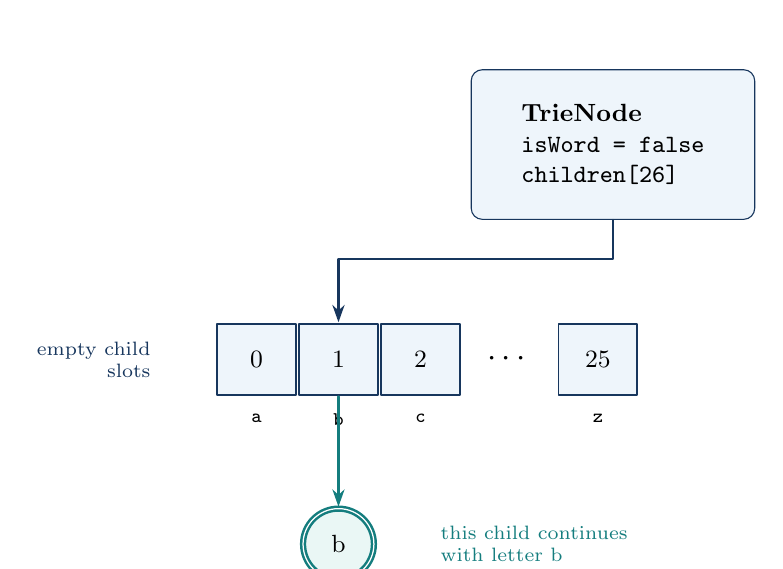
\begin{tikzpicture}[>={Stealth[length=2.2mm,width=1.55mm]},font=\small]
  \node[draw=navy,fill=softblue,rounded corners,minimum width=36mm,
        minimum height=19mm,align=left] (node) {
    \textbf{TrieNode}\\
    \texttt{isWord = false}\\
    \texttt{children[26]}
  };

  \node[arraycell,below left=13mm and 22mm of node] (ca) {0};
  \node[arraycell,right=0mm of ca] (cb) {1};
  \node[arraycell,right=0mm of cb] (cc) {2};
  \node[right=2mm of cc,font=\large] (dots) {$\cdots$};
  \node[arraycell,right=2mm of dots] (cz) {25};

  \node[below=1mm of ca,font=\scriptsize] {\texttt{a}};
  \node[below=1mm of cb,font=\scriptsize] {\texttt{b}};
  \node[below=1mm of cc,font=\scriptsize] {\texttt{c}};
  \node[below=1mm of cz,font=\scriptsize] {\texttt{z}};

  \draw[flowarrow] (node.south) -- ++(0,-5mm) -| (cb.north);
  \node[trienode,visited,below=14mm of cb] (next) {b};
  \draw[flowarrow,teal] (cb.south) -- (next.north);
  \node[right=7mm of next,align=left,font=\scriptsize,text=teal]
    {this child continues\\with letter b};
  \node[left=7mm of ca,align=right,font=\scriptsize,text=navy]
    {empty child\\slots};
\end{tikzpicture}

\smallskip
Each numbered slot stands for one letter. A used slot points to the next
letter. \texttt{isWord} tells us whether a complete word ends here.
\end{visualbox}

\subsection{Trie Node Structure}

\begin{lstlisting}
struct TrieNode {
    TrieNode* children[26];
    bool isWord;

    TrieNode() {
        isWord = false;

        for (int i = 0; i < 26; i++) {
            children[i] = nullptr;
        }
    }
};
\end{lstlisting}

A new node starts with every child pointer set to \texttt{nullptr} and
\texttt{isWord = false}. It has no outgoing character path and does not yet
mark the end of a stored word.

\subsection{Creating the Root}

We create the root of the Trie using:

\begin{lstlisting}
TrieNode* root = new TrieNode();
\end{lstlisting}

The root does not represent any particular character.

It serves as the starting point from which all words are stored.

\begin{visualbox}{Trie after adding \texttt{bad}, \texttt{dad}, and \texttt{mad}}
\centering
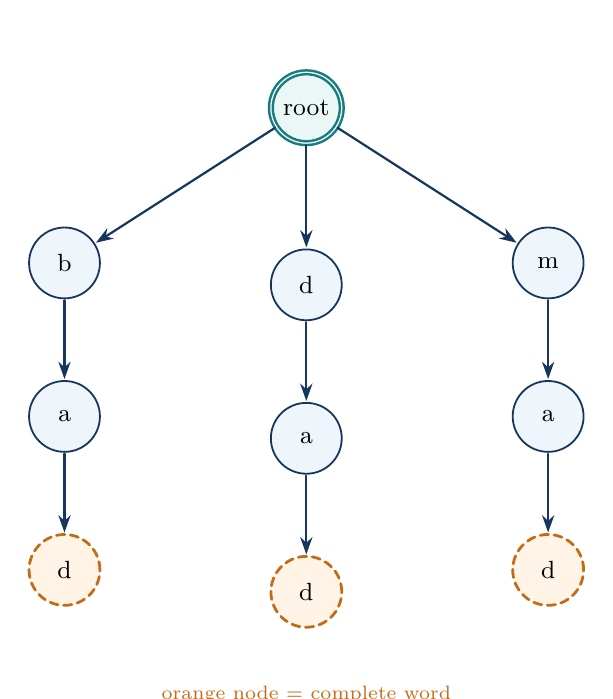
\begin{tikzpicture}[level distance=12mm,>={Stealth[length=2.2mm,width=1.55mm]},font=\small]
    \node[trienode,visited] (root) {root};
    \node[trienode,below left=13mm and 24mm of root] (b) {b};
    \node[trienode,below=13mm of root] (d) {d};
    \node[trienode,below right=13mm and 24mm of root] (m) {m};
    \node[trienode,below=10mm of b] (ba) {a};
    \node[trienode,below=10mm of d] (da) {a};
    \node[trienode,below=10mm of m] (ma) {a};
    \node[trienode,active,below=10mm of ba] (bad) {d};
    \node[trienode,active,below=10mm of da] (dad) {d};
    \node[trienode,active,below=10mm of ma] (mad) {d};
    \foreach \x/\y in {root/b,root/d,root/m,b/ba,d/da,m/ma,ba/bad,da/dad,ma/mad}
        \draw[flowarrow] (\x)--(\y);
    \node[below=6mm of dad,text=orange,font=\scriptsize]
      {orange node = complete word};
\end{tikzpicture}

The root holds no letter. Following the arrows spells each word. Orange nodes
show where a complete word ends.
\end{visualbox}

\subsection{Adding a Word}

To add a word, we start from the root node:

\begin{lstlisting}
TrieNode* node = root;
\end{lstlisting}

We then iterate through every character in the word.

For each character, we convert it into an index between \(0\) and
\(25\): \(\texttt{index}=c-'a'\)

This lets us access the matching child in the
\texttt{children} array.

For example: \(a\rightarrow0\) \(b\rightarrow1\) \(c\rightarrow2\)

and so on.

\subsection{Adding Characters to the Trie}

For every character \(c\), we check whether its matching child
node already exists.

If it does not exist, we create a new Trie node.

Conceptually:

\begin{lstlisting}
if (node->children[c - 'a'] == nullptr) {
    node->children[c - 'a'] = new TrieNode();
}
\end{lstlisting}

We then move to that child:

\begin{lstlisting}
node = node->children[c - 'a'];
\end{lstlisting}

This process continues until every character of the word has been
processed.

\subsection{Marking the End of a Word}

After processing all characters, we mark the current node as the
end of a word:

\begin{lstlisting}
node->isWord = true;
\end{lstlisting}

This is important because one word can be a prefix of another word.

For example, suppose we insert: \(\texttt{app}\)

and: \(\texttt{apple}\)

The node matching to the final character of \texttt{app} must
be marked as a complete word even though additional characters
continue afterward for \texttt{apple}.

\subsection{Search Operation}

To search for a word, we again start at the root:

\begin{lstlisting}
TrieNode* node = root;
\end{lstlisting}

We then process every character in the word.

For each character \(c\), we calculate: \(\texttt{index}=c-'a'\)

and check whether the matching child exists.

If the child does not exist, the word cannot be present in the Trie.

So, we return:

\begin{lstlisting}
false
\end{lstlisting}

If the child exists, we move to that node and continue searching.

After processing every character, we return:

\begin{lstlisting}
node->isWord
\end{lstlisting}

This ensures that the complete word exists rather than merely being
a prefix of another word.

\subsection{Why \texttt{isWord} Is Needed}

\begin{conceptbox}{A path is not automatically a word}
After inserting \texttt{apple}, the path
$a\rightarrow p\rightarrow p\rightarrow l\rightarrow e$ exists. That proves
\texttt{app} is a prefix, but it does not prove that \texttt{app} was inserted
as a complete word. The second \texttt{p} node must have
\texttt{isWord = true} before \texttt{search("app")} may return true.
\end{conceptbox}

The rule is simple: following child pointers proves that a path exists;
\texttt{isWord} proves that the path ends at a stored word.

\subsection{Complete Implementation}

\begin{lstlisting}
class WordDictionary {
public:

    struct TrieNode {
        TrieNode* children[26];
        bool isWord;

        TrieNode() {
            isWord = false;

            for (int i = 0; i < 26; i++) {
                children[i] = nullptr;
            }
        }
    };

    TrieNode* root;

    WordDictionary() {
        root = new TrieNode();
    }

    void addWord(string word) {
        TrieNode* node = root;

        for (char c : word) {
            int index = c - 'a';

            if (node->children[index] == nullptr) {
                node->children[index] = new TrieNode();
            }

            node = node->children[index];
        }

        node->isWord = true;
    }
};
\end{lstlisting}

\subsection{Search with a Recursive Helper}

The search operation becomes more interesting when the problem
allows a special character such as: \(\texttt{'.'}\)

The dot can represent any lowercase English character.

So, a normal character can be handled by following one
specific child, while a dot requires us to potentially explore all
\(26\) children.

We can handle this using recursion.

The recursive search function receives:

\begin{itemize}
    \item The current word.
    \item The current character index.
    \item The current Trie node.
\end{itemize}

Conceptually:

\begin{lstlisting}
bool search(string word) {
    return dfs(word, 0, root);
}
\end{lstlisting}

The recursive helper is:

\begin{lstlisting}
bool dfs(string word, int index, TrieNode* node)
\end{lstlisting}

\subsection{Base Case}

If we have reached the end of the word: \(\texttt{index == word.size()}\)

then we return whether the current node represents the end of a
complete word:

\begin{lstlisting}
return node->isWord;
\end{lstlisting}

\subsection{Normal Character}

If the current character is not a dot, we simply follow its
matching child.

If that child does not exist, we return: \(\texttt{false}\)

Otherwise, we recursively continue with the next character.

\subsection{Dot Character}

If the current character is: \(\texttt{'.'}\)

then it can represent any lowercase English letter.

So, we must try every possible child: \(0,1,2,\ldots,25\)

If any of these recursive searches returns \texttt{true}, then the
word exists.

Otherwise, we return \texttt{false}.

\begin{visualbox}{A dot tries every possible first letter}
\centering
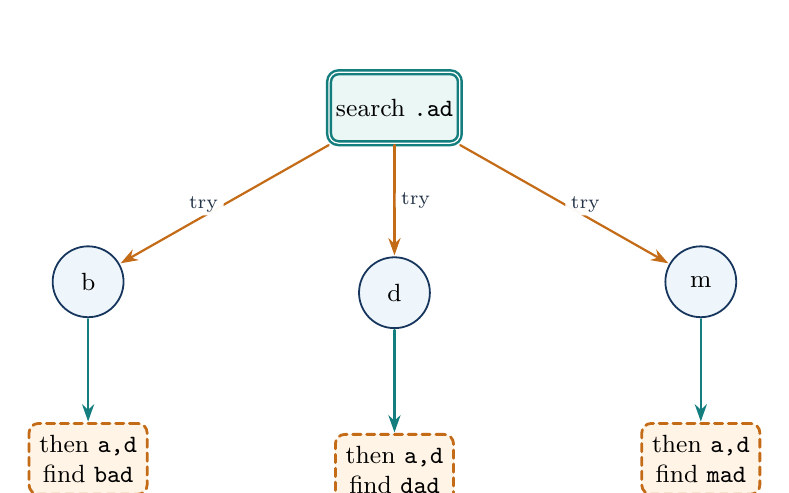
\begin{tikzpicture}[>={Stealth[length=2.2mm,width=1.55mm]},font=\small]
    \node[dsnode,visited] (query) {search \texttt{.ad}};
    \node[trienode,below left=14mm and 27mm of query] (b) {b};
    \node[trienode,below=14mm of query] (d) {d};
    \node[trienode,below right=14mm and 27mm of query] (m) {m};
    \draw[flowarrow,orange] (query)--node[edgelabel,left,font=\scriptsize]{try} (b);
    \draw[flowarrow,orange] (query)--node[edgelabel,right,font=\scriptsize]{try} (d);
    \draw[flowarrow,orange] (query)--node[edgelabel,right,font=\scriptsize]{try} (m);
    \node[dsnode,active,below=13mm of b] (bad) {then \texttt{a,d}\\find \texttt{bad}};
    \node[dsnode,active,below=13mm of d] (dad) {then \texttt{a,d}\\find \texttt{dad}};
    \node[dsnode,active,below=13mm of m] (mad) {then \texttt{a,d}\\find \texttt{mad}};
    \draw[flowarrow,teal] (b)--(bad);
    \draw[flowarrow,teal] (d)--(dad);
    \draw[flowarrow,teal] (m)--(mad);
\end{tikzpicture}

The dot may try any first letter. The letters \texttt{a} and \texttt{d} then
follow one path. The search stops when one complete word is found.
\end{visualbox}

\begin{visualbox}{Only one dot choice is tried at a time}
\centering
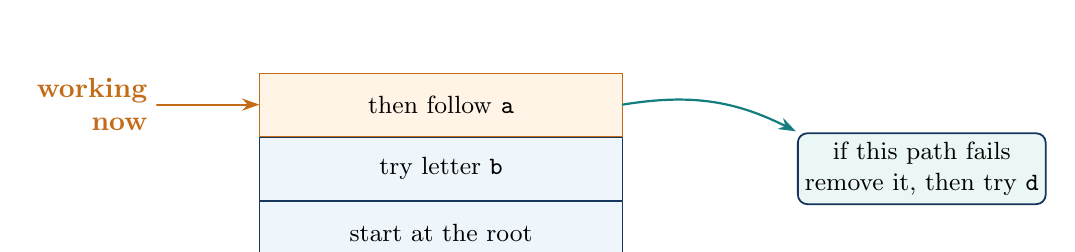
\begin{tikzpicture}[font=\small,>={Stealth[length=2.2mm,width=1.55mm]}]
  \node[draw=navy,fill=softblue,minimum width=46mm,minimum height=8mm] (f0)
    {start at the root};
  \node[draw=navy,fill=softblue,minimum width=46mm,minimum height=8mm,
    above=0mm of f0] (f1) {try letter \texttt{b}};
  \node[draw=orange,fill=softorange,minimum width=46mm,minimum height=8mm,
    above=0mm of f1] (f2) {then follow \texttt{a}};
  \node[left=13mm of f2,text=orange,font=\bfseries,align=right] (top) {working\\now};
  \draw[flowarrow,orange] (top)--(f2);
  \node[right=22mm of f1,dsnode,fill=softteal] (next)
    {if this path fails\\remove it, then try \texttt{d}};
  \draw[flowarrow,teal] (f2.east) to[bend left=18] (next.north west);
\end{tikzpicture}

\smallskip
Only the path being checked is kept on the stack. If it fails, remove that
path and try the next first letter.
\end{visualbox}

\subsection{Complete Search Code}

\begin{lstlisting}[style=compactcode]
using namespace std;

bool dfs(string word, int index, TrieNode* node) {

    if (index == word.size()) {
        return node->isWord;
    }

    char c = word[index];

    if (c == '.') {

        for (int i = 0; i < 26; i++) {

            if (node->children[i] != nullptr &&
                dfs(word, index + 1, node->children[i])) {
                return true;
            }
        }

        return false;

    } else {

        int childIndex = c - 'a';

        if (node->children[childIndex] == nullptr) {
            return false;
        }

        return dfs(
            word,
            index + 1,
            node->children[childIndex]
        );
    }
}
\end{lstlisting}

\subsection{Complete Data Structure}

Here is the complete version:

\begin{lstlisting}[style=longcode,caption={Complete C++ data structure: Word Dictionary}]
#include <string>

using namespace std;

class WordDictionary {
public:
    struct TrieNode {
        TrieNode* children[26];
        bool isWord;
        TrieNode() : isWord(false) {
            for (int i = 0; i < 26; ++i) children[i] = nullptr;
        }
    };
    TrieNode* root;
    WordDictionary() : root(new TrieNode()) {}
    void addWord(const string& word) {
        TrieNode* node = root;
        for (char c : word) {
            const int index = c - 'a';
            if (node->children[index] == nullptr) {
                node->children[index] = new TrieNode();
            }
            node = node->children[index];
        }
        node->isWord = true;
    }
    bool search(const string& word) {
        return dfs(word, 0, root);
    }
private:
    bool dfs(const string& word, int index, TrieNode* node) {
        if (index == static_cast<int>(word.size())) {
            return node->isWord;
        }
        const char c = word[index];
        if (c == '.') {
            for (int i = 0; i < 26; ++i) {
                if (node->children[i] != nullptr &&
                    dfs(word, index + 1, node->children[i])) {
                    return true;
                }
            }
            return false;
        }
        const int childIndex = c - 'a';
        if (node->children[childIndex] == nullptr) return false;
        return dfs(word, index + 1, node->children[childIndex]);
    }
};
\end{lstlisting}

\subsection{Time and Space}

Let \(L\) be the pattern length and \(d\) the number of wildcard positions.
Adding a word takes \(O(L)\) time. A search without wildcards also takes
\(O(L)\) time. With wildcards, the most useful exact description is
\(O(V_L)\), where \(V_L\) is the number of Trie states actually visited up to
depth \(L\). A loose worst-case upper bound is \(O(26^dL)\) for a dense Trie.
The recursive call stack uses \(O(L)\) space, while the Trie itself uses space
based on the total number of stored characters.

\subsection{Key Idea}

Here is the whole idea:

\begin{enumerate}
    \item Use a Trie to store all words.
    \item Each node has \(26\) possible children.
    \item Use \texttt{isWord} to identify the end of a complete word.
    \item For normal characters, follow one specific child.
    \item For \texttt{'.'}, recursively try all possible children.
\end{enumerate}

The Trie allows words to be stored and searched character by
character, while recursion allows the search to branch whenever a
wildcard character is seen.

\subsection{Detailed Visual Dry Run}

\begin{dryrunbox}{Add \texttt{bad}, \texttt{dad}, and \texttt{mad}; then search \texttt{.ad}}
\begin{center}
\small
\begin{tabularx}{\linewidth}{@{}c p{3.0cm} X@{}}
\toprule
Step & Operation & What happens \\
\midrule
1 & \texttt{addWord("bad")} & Create the path root \(\to b\to a\to d\), then mark the final node as a word. \\
2 & \texttt{addWord("dad")} & Create root \(\to d\to a\to d\). The earlier word stays unchanged. \\
3 & \texttt{addWord("mad")} & Create root \(\to m\to a\to d\). \\
4 & \texttt{search(".ad")} & The dot tries the root's children. The \(b\) branch follows \(a,d\) and reaches a word end, so the search stops with \texttt{true}. \\
\bottomrule
\end{tabularx}
\end{center}
\end{dryrunbox}

\chaptercheckpoint
  {Stored words share prefixes and a wildcard may match several children.}
  {Trie nodes, end markers, and a DFS position/node pair.}
  {Following only one child for a dot or accepting a prefix as a complete word.}
  {$O(L)$ ordinary search; wildcard search is based on visited Trie states.}

% =================================================
% IMPLEMENT TRIE (PREFIX TREE)
% =================================================

\problemstart{Implement Trie (Prefix Tree)}{208}{Medium}{Prefix tree}{Trie}

\subsection{The Problem}

Build a prefix-tree class with four operations:

\begin{enumerate}
    \item \texttt{Trie()} -- Create an empty Trie.
    \item \texttt{insert(word)} -- Store a word in the Trie.
    \item \texttt{search(word)} -- Return \texttt{true} if the complete
    word exists in the Trie.
    \item \texttt{startsWith(prefix)} -- Return \texttt{true} if at
    least one stored word starts with the given prefix.
\end{enumerate}

The words contain only lowercase English letters: \(\texttt{'a'} \text{ to } \texttt{'z'}\)

\subsection{Important Observation}

A prefix is not necessarily a complete word.

For example, suppose we insert: \(\texttt{"apple"}\)

Then: \(\texttt{search("app")}=\texttt{false}\)

because \texttt{"app"} was not inserted as a complete word.

However, \(\texttt{startsWith("app")}=\texttt{true}\)

because \texttt{"apple"} starts with the prefix \texttt{"app"}.

This distinction is important when designing the Trie.

% =================================================
% WHAT IS A TRIE?
% =================================================

\subsection{What is a Trie?}

A \textbf{Trie}, also called a \textbf{Prefix Tree}, is a tree-based
data structure used to store strings.

Instead of storing an entire word inside a single node, a Trie stores
the word character by character.

For example, consider the words: \(\texttt{"app"}\)

and \(\texttt{"apple"}\)

Both words reuse the same nodes for the shared prefix \texttt{app}.
The longer word continues from that node through \texttt{l} and \texttt{e}.

The path: \(a\rightarrow p\rightarrow p\)

represents the word \texttt{"app"}.

The path: \(a\rightarrow p\rightarrow p\rightarrow l\rightarrow e\)

represents the word \texttt{"apple"}.

\begin{visualbox}{The words \texttt{app} and \texttt{apple} share the same beginning}
\centering
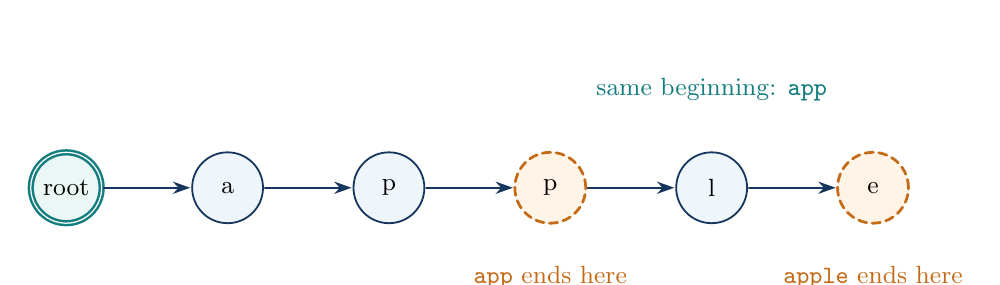
\begin{tikzpicture}[>={Stealth[length=2.2mm,width=1.55mm]},font=\small,node distance=11mm]
    \node[trienode,visited] (root) {root};
    \node[trienode,right=of root] (a) {a};
    \node[trienode,right=of a] (p1) {p};
    \node[trienode,active,right=of p1] (p2) {p};
    \node[trienode,right=of p2] (l) {l};
    \node[trienode,active,right=of l] (e) {e};
    \draw[flowarrow] (root)--(a);
    \draw[flowarrow] (a)--(p1);
    \draw[flowarrow] (p1)--(p2);
    \draw[flowarrow] (p2)--(l);
    \draw[flowarrow] (l)--(e);
    \node[below=4mm of p2,text=orange,align=center] {\texttt{app} ends here};
    \node[below=4mm of e,text=orange,align=center] {\texttt{apple} ends here};
    \node[above=5mm of l,text=teal] {same beginning: \texttt{app}};
\end{tikzpicture}

\texttt{search("app")} checks that a word ends at the second \texttt{p}.
\texttt{startsWith("app")} only checks that the letters can be followed.
\end{visualbox}

\begin{invariantbox}{the current node represents exactly the consumed prefix}
After consuming the first \(k\) characters, the current pointer is the Trie
node for that length-\(k\) prefix. Reaching a node proves the prefix exists;
only \texttt{isWord=true} proves it was inserted as a complete word.
\end{invariantbox}

\subsection{Why Do We Need an End Marker?}

Consider inserting: \(\texttt{"apple"}\)

The nodes for: \(a\rightarrow p\rightarrow p\)

already exist as part of the word.

However, this does not mean that: \(\texttt{"app"}\)

is a complete word.

So, every Trie node needs a Boolean variable: \(\texttt{isWord}\)

which tells us whether the current node represents the end of a
complete word.

If both \texttt{"app"} and \texttt{"apple"} were inserted, the second
\texttt{p} node and the final \texttt{e} node each have
\texttt{isWord = true}. The vector diagram above shows these two endings
without mixing tree structure with ASCII art.

% =================================================
% TRIE NODE
% =================================================

\subsection{Trie Node}

Each Trie node contains:

\begin{itemize}
    \item An array of \(26\) child pointers.
    \item A Boolean variable \texttt{isWord}.
\end{itemize}

The \(26\) children correspond to: \(a,b,c,\ldots,z\)

So, each node can have at most \(26\) children.

\subsection{Trie Node Implementation}

\begin{lstlisting}
struct TrieNode {

    TrieNode* children[26];

    bool isWord;

    TrieNode() {

        isWord = false;

        for (int i = 0; i < 26; i++) {
            children[i] = nullptr;
        }
    }
};
\end{lstlisting}

A newly constructed node has 26 null child pointers and
\texttt{isWord = false}. Connections and word endings are added only during
insertion.

% =================================================
% ROOT
% =================================================

\subsection{Root Node}

We create a root node for the Trie.

\begin{lstlisting}
TrieNode* root = new TrieNode();
\end{lstlisting}

The root node does not represent any character.

It simply acts as the starting point from which all words are
stored.

The root is a sentinel node: it stores no character. Its child pointers lead
to the first letters of the stored words, and every later edge represents the
next character in a path.

% =================================================
% INSERT
% =================================================

\subsection{Insert Operation}

The purpose of the \texttt{insert()} operation is to store a word in
the Trie.

Suppose we want to insert: \(\texttt{"apple"}\)

We start from the root and process every character one by one.

The path becomes: \(root \rightarrow a \rightarrow p \rightarrow p \rightarrow l \rightarrow e\)

\begin{visualbox}{Adding \texttt{apple} reuses \texttt{app} and adds \texttt{l,e}}
\centering
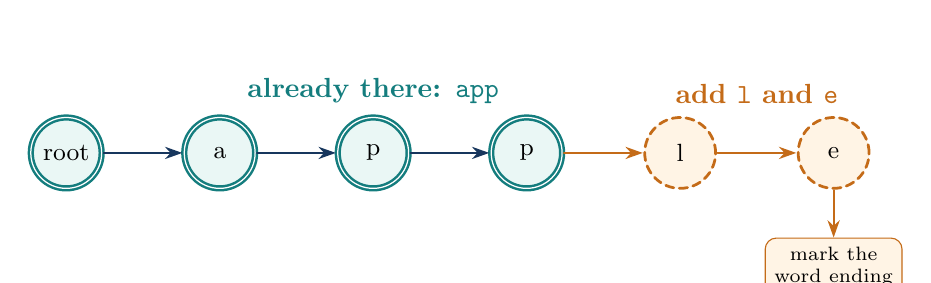
\begin{tikzpicture}[>={Stealth[length=2.2mm,width=1.55mm]},font=\small,node distance=10mm]
  \node[trienode,visited] (root) {root};
  \node[trienode,visited,right=of root] (a) {a};
  \node[trienode,visited,right=of a] (p1) {p};
  \node[trienode,visited,right=of p1] (p2) {p};
  \node[trienode,active,right=of p2] (l) {l};
  \node[trienode,active,right=of l] (e) {e};
  \draw[flowarrow] (root)--(a);
  \draw[flowarrow] (a)--(p1);
  \draw[flowarrow] (p1)--(p2);
  \draw[flowarrow,orange] (p2)--(l);
  \draw[flowarrow,orange] (l)--(e);
  \node[above=5mm of $(a)!0.5!(p2)$,text=teal,font=\bfseries]
    {already there: \texttt{app}};
  \node[above=5mm of $(l)!0.5!(e)$,text=orange,font=\bfseries]
    {add \texttt{l} and \texttt{e}};
  \node[below=6mm of e,draw=orange,fill=softorange,rounded corners,
        align=center,font=\scriptsize] (mark) {mark the\\word ending};
  \draw[flowarrow,orange] (e)--(mark);
\end{tikzpicture}

\smallskip
Follow letters that are already present. Add a new circle only for a missing
letter, then mark where the complete word ends.
\end{visualbox}

\subsubsection{Character to Index Conversion}

Since every node contains an array of \(26\) children, we convert a
character into an index using: \(\boxed{\texttt{index}=c-\texttt{'a'}}\)

For example: \(\texttt{'a'}-\texttt{'a'}=0\) \(\texttt{'b'}-\texttt{'a'}=1\) \(\texttt{'c'}-\texttt{'a'}=2\)

and so on.

So: \(\texttt{'z'}-\texttt{'a'}=25\)

\subsubsection{Creating Missing Nodes}

For every character, we check whether the matching child
already exists.

If it does not exist, we create a new node:

\begin{lstlisting}
if (node->children[index] == nullptr) {
    node->children[index] = new TrieNode();
}
\end{lstlisting}

Then we move to that child:

\begin{lstlisting}
node = node->children[index];
\end{lstlisting}

This process continues until every character of the word has been
processed.

\subsubsection{Marking the End of the Word}

After processing the final character, we mark the current node as the
end of a complete word:

\begin{lstlisting}
node->isWord = true;
\end{lstlisting}

This is what allows the Trie to distinguish between a complete word
and merely a prefix.

% =================================================
% INSERT CODE
% =================================================

\subsection{Insert Implementation}

\begin{lstlisting}
void insert(string word) {

    TrieNode* node = root;

    for (char c : word) {

        int index = c - 'a';

        if (node->children[index] == nullptr) {
            node->children[index] = new TrieNode();
        }

        node = node->children[index];
    }

    node->isWord = true;
}
\end{lstlisting}

% =================================================
% SEARCH
% =================================================

\subsection{Search Operation}

The purpose of \texttt{search()} is to determine whether the
\textbf{complete word} exists in the Trie.

Suppose we search for: \(\texttt{"apple"}\)

We start from the root and follow: \(a\rightarrow p\rightarrow p\rightarrow l\rightarrow e\)

If at any point the required child does not exist, the word does not
exist.

So, we immediately return: \(\texttt{false}\)

If we successfully process every character, we still need to check: \(\texttt{isWord}\)

This is because the searched string may only be a prefix of a stored
word.

\subsection{Search Implementation}

\begin{lstlisting}
bool search(string word) {

    TrieNode* node = root;

    for (char c : word) {

        int index = c - 'a';

        if (node->children[index] == nullptr) {
            return false;
        }

        node = node->children[index];
    }

    return node->isWord;
}
\end{lstlisting}

% =================================================
% STARTS WITH
% =================================================

\subsection{\texttt{startsWith()} Operation}

The third operation is:

\begin{lstlisting}
startsWith(prefix)
\end{lstlisting}

Its purpose is to determine whether at least one word stored in the
Trie begins with the given prefix.

For example, if the Trie contains: \(\texttt{"apple"}\)

then: \(\texttt{startsWith("app")}=\texttt{true}\)

because \texttt{"apple"} begins with \texttt{"app"}.

However, unlike \texttt{search()}, we do \textbf{not} need to check
\texttt{isWord} at the end.

We only need to determine whether the complete prefix path exists.

\begin{visualbox}{\texttt{search} and \texttt{startsWith} stop differently}
\centering
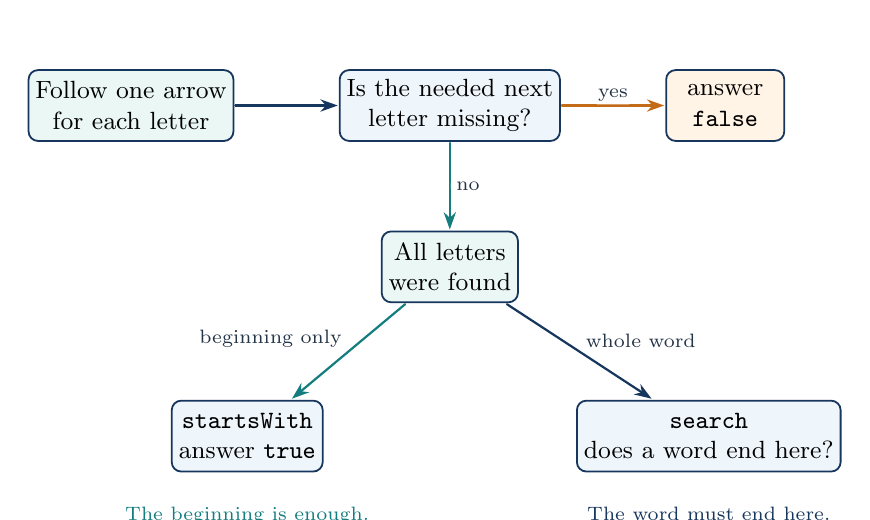
\begin{tikzpicture}[>={Stealth[length=2.2mm,width=1.55mm]},font=\small,node distance=8mm]
  \node[dsnode,fill=softteal] (walk) {Follow one arrow\\for each letter};
  \node[dsnode,right=13mm of walk] (missing) {Is the needed next\\letter missing?};
  \draw[flowarrow] (walk)--(missing);
  \node[dsnode,fill=softorange,right=13mm of missing] (false) {answer\\\texttt{false}};
  \draw[flowarrow,orange] (missing)--node[edgelabel,above,font=\scriptsize]{yes} (false);

  \node[dsnode,fill=softteal,below=11mm of missing] (complete)
    {All letters\\were found};
  \draw[flowarrow,teal] (missing)--node[edgelabel,right,font=\scriptsize]{no} (complete);

  \node[dsnode,below left=12mm and 7mm of complete] (prefix) {
    \texttt{startsWith}\\answer \texttt{true}};
  \node[dsnode,below right=12mm and 7mm of complete] (word) {
    \texttt{search}\\does a word end here?};
  \draw[flowarrow,teal] (complete) --
    node[edgelabel,above left,font=\scriptsize]{beginning only} (prefix);
  \draw[flowarrow] (complete) --
    node[edgelabel,above right,font=\scriptsize]{whole word} (word);
  \node[below=3mm of prefix,font=\scriptsize,text=teal,align=center]
    {The beginning is enough.};
  \node[below=3mm of word,font=\scriptsize,text=navy,align=center]
    {The word must end here.};
\end{tikzpicture}
\end{visualbox}

% =================================================
% STARTS WITH IMPLEMENTATION
% =================================================

\subsection{\texttt{startsWith()} Implementation}

\begin{lstlisting}
bool startsWith(string prefix) {

    TrieNode* node = root;

    for (char c : prefix) {

        int index = c - 'a';

        if (node->children[index] == nullptr) {
            return false;
        }

        node = node->children[index];
    }

    return true;
}
\end{lstlisting}

% =================================================
% COMPLETE IMPLEMENTATION
% =================================================

\subsection{Complete Implementation}

\begin{lstlisting}[style=compactcode,caption={Complete C++ data structure: Trie}]
#include <string>

using namespace std;

class Trie {
public:
    struct TrieNode {
        TrieNode* children[26];
        bool isWord;
        TrieNode() : isWord(false) {
            for (int i = 0; i < 26; ++i) children[i] = nullptr;
        }
    };
    TrieNode* root;
    Trie() : root(new TrieNode()) {}
    void insert(const string& word) {
        TrieNode* node = root;
        for (char c : word) {
            const int index = c - 'a';
            if (node->children[index] == nullptr) {
                node->children[index] = new TrieNode();
            }
            node = node->children[index];
        }
        node->isWord = true;
    }
    bool search(const string& word) {
        TrieNode* node = root;
        for (char c : word) {
            const int index = c - 'a';
            if (node->children[index] == nullptr) return false;
            node = node->children[index];
        }
        return node->isWord;
    }
    bool startsWith(const string& prefix) {
        TrieNode* node = root;
        for (char c : prefix) {
            const int index = c - 'a';
            if (node->children[index] == nullptr) return false;
            node = node->children[index];
        }
        return true;
    }
};
\end{lstlisting}

% =================================================
% EXAMPLE
% =================================================

\subsection{Example Walkthrough}

Suppose we perform:

\begin{lstlisting}
Trie trie;

trie.insert("apple");
\end{lstlisting}

The Trie contains the path: \(a\rightarrow p\rightarrow p\rightarrow l\rightarrow e\)

and the final node has: \(\texttt{isWord}=\texttt{true}\)

Now consider:

\begin{lstlisting}
trie.search("apple");
\end{lstlisting}

The complete path exists and the final node has
\texttt{isWord = true}, so: \(\boxed{\texttt{true}}\)

Now:

\begin{lstlisting}
trie.search("app");
\end{lstlisting}

The path exists, but if \texttt{"app"} was not inserted separately,
the node has: \(\texttt{isWord}=\texttt{false}\)

So: \(\boxed{\texttt{false}}\)

However:

\begin{lstlisting}
trie.startsWith("app");
\end{lstlisting}

returns: \(\boxed{\texttt{true}}\)

because the prefix path exists.

% =================================================
% SEARCH VS STARTSWITH
% =================================================

\subsection{\texttt{search()} vs \texttt{startsWith()}}

The main difference is:

\begin{center}
\renewcommand{\arraystretch}{1.4}
\begin{tabular}{|c|c|c|}
\hline
\textbf{Operation} & \textbf{What it checks} & \textbf{Uses \texttt{isWord}?} \\
\hline
\texttt{search()} &
Complete word exists &
Yes \\
\hline
\texttt{startsWith()} &
Prefix path exists &
No \\
\hline
\end{tabular}
\end{center}

This distinction is one of the most important concepts in the
problem.

% =================================================
% COMPLEXITY
% =================================================

\subsection{Time and Space}

Let \(L\) be the length of the word or prefix.

For \texttt{insert()}, we process every character exactly once: \(\boxed{O(L)}\)

For \texttt{search()}, we also process every character at most once: \(\boxed{O(L)}\)

For \texttt{startsWith()}, the same applies: \(\boxed{O(L)}\)

So:

\[
\boxed{
\begin{aligned}
\text{Insert} &= O(L)\\
\text{Search} &= O(L)\\
\text{StartsWith} &= O(L)
\end{aligned}
}
\]

The space required by the Trie depends on the total number of
characters inserted.

If the total number of inserted characters is \(N\), the Trie can
use: \(\boxed{O(N)}\)

nodes in the worst case.

% =================================================
% KEY TAKEAWAYS
% =================================================

\subsection{Key Takeaways}

\begin{itemize}
    \item A Trie is also called a Prefix Tree.
    \item A Trie stores words character by character.
    \item Each node contains \(26\) child pointers for lowercase
    English letters.
    \item \texttt{isWord} identifies whether a node represents the
    end of a complete word.
    \item \texttt{search()} checks both the path and
    \texttt{isWord}.
    \item \texttt{startsWith()} only checks whether the prefix path
    exists.
    \item Character-to-index conversion is performed using:
    \(c-\texttt{'a'}\)
    \item Insert, search, and prefix operations take:
    \(O(L)\)
    time, where \(L\) is the length of the input string.
\end{itemize}

\subsection{Detailed Visual Dry Run}

\begin{dryrunbox}{Insert \texttt{apple}, then compare \texttt{search} with \texttt{startsWith}}
\begin{center}
\small
\begin{tabularx}{\linewidth}{@{}c p{4.0cm} X@{}}
\toprule
Step & Operation & What happens \\
\midrule
1 & \texttt{insert("apple")} & Walk through \(a,p,p,l,e\), creating missing nodes. Mark only the \(e\) node as a complete word. \\
2 & \texttt{search("apple")} & The whole path exists and the final node is marked, so return \texttt{true}. \\
3 & \texttt{search("app")} & The path exists, but the second \(p\) node is not a word end, so return \texttt{false}. \\
4 & \texttt{startsWith("app")} & The same path exists. A prefix does not need a word-end mark, so return \texttt{true}. \\
\bottomrule
\end{tabularx}
\end{center}
\end{dryrunbox}

\chaptercheckpoint
  {Many operations repeatedly query complete words and shared prefixes.}
  {Character-child links and an end-of-word Boolean at each Trie node.}
  {Making \texttt{search} and \texttt{startsWith} use the same final condition.}
  {$O(L)$ per operation and $O(N)$ total stored-node space.}

% =================================================
% ALIEN DICTIONARY
% =================================================

\patternintoc{Graph Patterns}
\problemstart{Alien Dictionary}{269}{Hard}{Topological sorting}{Directed graph and queue}

\subsection{The Problem}

A list of words has already been sorted using an unknown alphabet order.
Recover one character order consistent with that list. Return an empty string
if the comparisons imply a contradiction; when several orders are possible,
any valid one is acceptable.

\subsection{Input and Output}

The input is: \(\texttt{vector<string> words}\)

where the words are already sorted according to the unknown alien
language.

The output is: \(\texttt{string}\)

containing the unique characters in their valid alien-language
ordering.

If no valid ordering exists: \(\boxed{\texttt{""}}\)

If multiple valid orderings exist, any valid ordering is acceptable.

% =================================================
% LEXICOGRAPHICAL ORDER
% =================================================

\subsection{Understanding Dictionary Order}

Dictionary order compares two strings from left to right. The first
position where they differ decides which word comes first. For example,
\texttt{ape} comes before \texttt{apple}: the shared prefix is \texttt{ap},
then \texttt{e} comes before \texttt{p}.

\begin{conceptbox}{Only the first difference matters}
\centering
\begin{tabular}{c c c c}
\texttt{a} & \texttt{p} & \textcolor{orange}{\texttt{e}} & \\
$=$ & $=$ & $<$ & \\
\texttt{a} & \texttt{p} & \textcolor{navy}{\texttt{p}} & \texttt{l e}
\end{tabular}

\smallskip
So, \(\texttt{ape}<\texttt{apple}\).
\end{conceptbox}

The same concept is used in the alien dictionary, except that the
ordering of the characters is unknown.

% =================================================
% MAIN IDEA
% =================================================

\subsection{Main Idea}

The ordering of adjacent words reveals ordering between characters. Compare
\texttt{abc} and \texttt{axc}. Their first characters match. The first
difference is \texttt{b} versus \texttt{x}, so the alien alphabet must place
\texttt{b} before \texttt{x}. \(\texttt{abc}<\texttt{axc} \quad\Longrightarrow\quad b<x \quad\Longrightarrow\quad b\rightarrow x\)

This gives us a directed relationship: \(b\longrightarrow x\)

So, the problem can be converted into a
\textbf{directed graph}.

% =================================================
% GRAPH REPRESENTATION
% =================================================

\subsection{Graph Representation}

Each unique character is represented as a node in the graph.

If we discover that: \(a<b\)

we create a directed edge: \(a\longrightarrow b\)

The meaning is: \(\boxed{ a\text{ must appear before }b }\)

After constructing all such relationships, we need to find an ordering
of the graph in which every directed edge goes from an earlier
character to a later character.

This is exactly the purpose of: \(\boxed{\text{Topological Sorting}}\)

% =================================================
% KAHN'S ALGORITHM
% =================================================

\subsection{Kahn's Algorithm}

We use \textbf{Kahn's algorithm} to perform topological sorting.

The algorithm is based on the concept of: \(\boxed{\text{Indegree}}\)

The indegree of a node is the number of edges coming into that node.

For example, if: \(a\rightarrow c\)

and: \(b\rightarrow c\)

then: \(\operatorname{indegree}(c)=2\)

because two characters must appear before \(c\).

Characters with: \(\operatorname{indegree}=0\)

can be placed at the beginning of the ordering.

\begin{invariantbox}{the queue contains exactly the available characters}
Every queued character has zero remaining indegree and has not yet been placed
in the result. Removing one character deletes its outgoing rules; a
neighbor is enqueued exactly when its final unmet rule disappears.
\end{invariantbox}

% =================================================
% IMPORTANT STEPS
% =================================================

\subsection{Algorithm Steps}

The solution can be divided into four major steps.

\subsubsection{Step 1: Start the Graph}

Create:

\begin{itemize}
    \item An adjacency list for the graph.
    \item An indegree array/map for all characters.
\end{itemize}

Since the alien language uses lowercase English letters, there can
be at most \(26\) possible characters.

We also need to make sure that every character appearing in the input
is represented in the graph, even if its indegree is zero.

\begin{visualbox}{What we save while building the letter order}
\centering
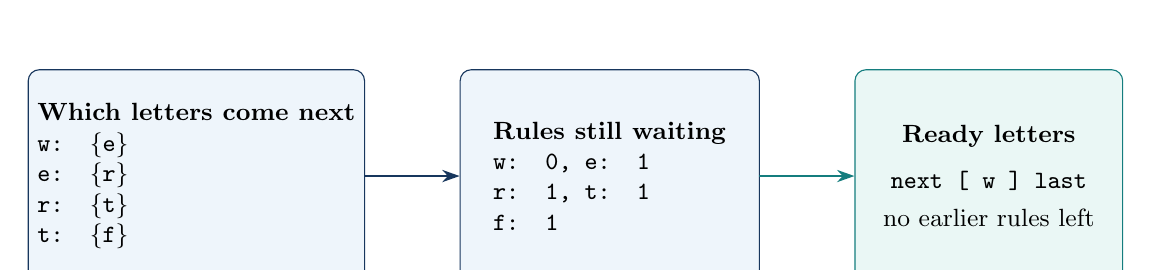
\begin{tikzpicture}[>={Stealth[length=2.2mm,width=1.55mm]},font=\small]
  \node[draw=navy,fill=softblue,rounded corners,minimum width=38mm,
        minimum height=27mm,align=left] (adj) {
    \textbf{Which letters come next}\\
    \texttt{w: \{e\}}\\
    \texttt{e: \{r\}}\\
    \texttt{r: \{t\}}\\
    \texttt{t: \{f\}}
  };
  \node[draw=navy,fill=softblue,rounded corners,minimum width=38mm,
        minimum height=27mm,align=left,right=12mm of adj] (degree) {
    \textbf{Rules still waiting}\\
    \texttt{w: 0, e: 1}\\
    \texttt{r: 1, t: 1}\\
    \texttt{f: 1}
  };
  \node[draw=teal,fill=softteal,rounded corners,minimum width=34mm,
        minimum height=27mm,align=center,right=12mm of degree] (queue) {
    \textbf{Ready letters}\\[2mm]
    \texttt{next [ w ] last}\\[1mm]
    no earlier rules left
  };
  \draw[flowarrow] (adj)--(degree);
  \draw[flowarrow,teal] (degree)--(queue);
\end{tikzpicture}

\smallskip
The first box shows which letter must follow another. The second counts how
many earlier-letter rules remain. The last box holds letters ready to use.
\end{visualbox}

% =================================================
% STEP 2
% =================================================

\subsubsection{Step 2: Build the Directed Graph}

We compare every pair of adjacent words. For \(i=0,1,\ldots,n-2\), let
\(\texttt{word1=words[i]}\)

and: \(\texttt{word2=words[i+1]}\)

We compare their characters from left to right.

Let \(j\) represent the character position.

As long as: \(\texttt{word1[j]}=\texttt{word2[j]}\)

there is no ordering information, so we continue.

When we find the first different pair: \(\texttt{word1[j]}\neq\texttt{word2[j]}\)

we have discovered an ordering relationship.

If: \(\texttt{word1[j]}=a\)

and: \(\texttt{word2[j]}=b\)

then: \(\boxed{a\rightarrow b}\)

and: \(\operatorname{indegree}(b)++\)

After finding the first different character, we stop comparing the
two words because later characters provide no additional information
about their dictionary ordering.

% =================================================
% PREFIX EDGE CASE
% =================================================

\subsection{Important Edge Case: Invalid Prefix}

There is an important invalid case.

Consider: \(\texttt{["abc","ab"]}\)

The first word is longer than the second word, but the second word is
a complete prefix of the first.

This ordering is impossible in dictionary order.

So, if: \(|\texttt{word1}|>|\texttt{word2}|\)

and all characters of \texttt{word2} match the beginning of
\texttt{word1}, then the input is invalid.

We return: \(\boxed{\texttt{""}}\)

\begin{visualbox}{A longer word cannot come before its own beginning}
\centering
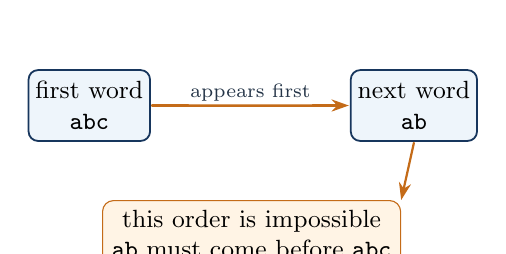
\begin{tikzpicture}[>={Stealth[length=2.2mm,width=1.55mm]},font=\small]
    \node[dsnode] (first) {first word\\\texttt{abc}};
    \node[dsnode,right=25mm of first] (second) {next word\\\texttt{ab}};
    \draw[flowarrow,orange] (first)--node[edgelabel,above]{appears first} (second);
    \node[draw=orange,fill=softorange,rounded corners,below=12mm of $(first)!0.5!(second)$,align=center]
        (invalid) {this order is impossible\\\texttt{ab} must come before \texttt{abc}};
    \draw[flowarrow,orange] (second.south)--(invalid.north east);
\end{tikzpicture}
\end{visualbox}

% =================================================
% STEP 3
% =================================================

\subsubsection{Step 3: Start the Queue}

After constructing the graph, we look for all characters whose
indegree is zero.

These characters have no dependencies.

So, they can appear at the beginning of the ordering.

We add them to a queue:

\begin{lstlisting}
queue<char> q;
\end{lstlisting}

For every character \(c\):

\begin{lstlisting}
if (indegree[c] == 0) {
    q.push(c);
}
\end{lstlisting}

% =================================================
% STEP 4
% =================================================

\subsubsection{Step 4: Perform Topological Sort}

While the queue is not empty:

\begin{enumerate}
    \item Remove one character from the queue.
    \item Add it to the result.
    \item Visit all of its neighboring characters.
    \item Decrease their indegree by one.
    \item If a neighbor's indegree becomes zero, add it to the queue.
\end{enumerate}

Conceptually, take a node, append it to the result, remove its outgoing
dependencies, and enqueue any nodes that have become available.

\begin{visualbox}{Take a ready letter, then unlock the next one}
\centering
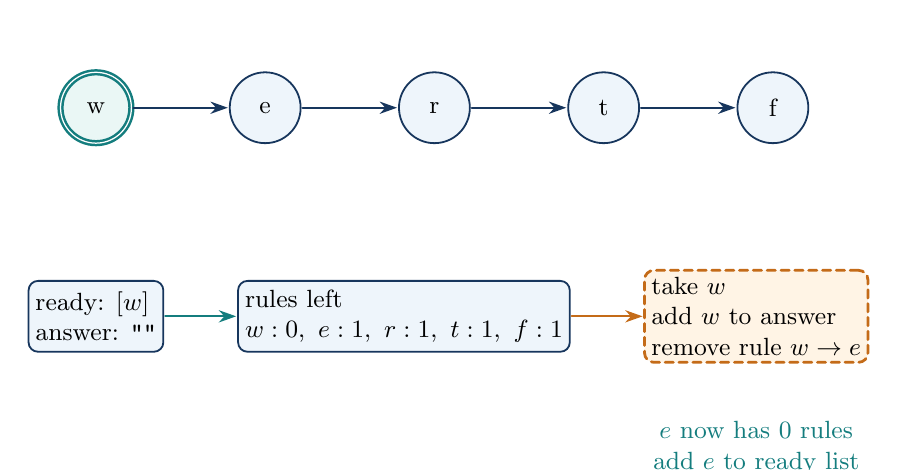
\begin{tikzpicture}[>={Stealth[length=2.2mm,width=1.55mm]},font=\small,node distance=12mm]
    \node[trienode,visited] (w) {w};
    \node[trienode,right=of w] (e) {e};
    \node[trienode,right=of e] (r) {r};
    \node[trienode,right=of r] (t) {t};
    \node[trienode,right=of t] (f) {f};
    \draw[flowarrow] (w)--(e);
    \draw[flowarrow] (e)--(r);
    \draw[flowarrow] (r)--(t);
    \draw[flowarrow] (t)--(f);

    \node[dsnode,below=17mm of w,align=left] (queue) {ready: $[w]$\\answer: \texttt{""}};
    \node[dsnode,right=9mm of queue,align=left] (degrees) {
        rules left\\$w:0,\ e:1,\ r:1,\ t:1,\ f:1$
    };
    \node[dsnode,active,right=9mm of degrees,align=left] (update) {
        take $w$\\add $w$ to answer\\remove rule $w\to e$
    };
    \draw[flowarrow,teal] (queue)--(degrees);
    \draw[flowarrow,orange] (degrees)--(update);
    \node[below=6mm of update,text=teal,align=center] {
        $e$ now has $0$ rules\\add $e$ to ready list
    };
\end{tikzpicture}

A letter becomes ready only after every letter that must come before it has
been used. In a cycle, some letters never become ready.
\end{visualbox}

% =================================================
% EXAMPLE
% =================================================

\subsection{Example}

Consider
\texttt{["wrt", "wrf", "er", "ett", "rftt"]}. Compare only adjacent
words and stop at each pair's first different character.

\begin{dryrunbox}{Building the character rules}
\begin{center}
\begin{tabular}{@{}lll@{}}
\toprule
Adjacent pair & First difference & Rule \\
\midrule
\texttt{wrt}, \texttt{wrf} & \texttt{t} versus \texttt{f} & $t\rightarrow f$ \\
\texttt{wrf}, \texttt{er} & \texttt{w} versus \texttt{e} & $w\rightarrow e$ \\
\texttt{er}, \texttt{ett} & \texttt{r} versus \texttt{t} & $r\rightarrow t$ \\
\texttt{ett}, \texttt{rftt} & \texttt{e} versus \texttt{r} & $e\rightarrow r$ \\
\bottomrule
\end{tabular}
\end{center}
\end{dryrunbox}

These edges form the chain
$w\rightarrow e\rightarrow r\rightarrow t\rightarrow f$, so one valid
answer is \texttt{"wertf"}.

% =================================================
% GRAPH
% =================================================

\subsection{Graph Structure}

The relationships can be visualized as: \(w\longrightarrow e\longrightarrow r \longrightarrow t\longrightarrow f\)

The topological ordering of this graph gives: \(\boxed{w,e,r,t,f}\)

which corresponds to: \(\boxed{\texttt{"wertf"}}\)

\begin{visualbox}{The letter rules form one clear order}
\centering
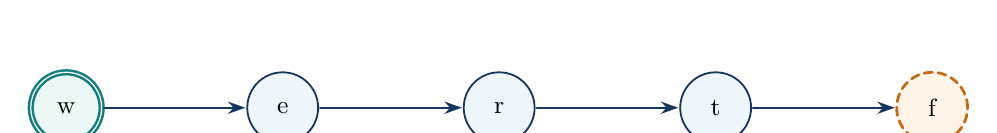
\begin{tikzpicture}[>={Stealth[length=2.2mm,width=1.55mm]},font=\small,node distance=18mm]
    \node[trienode,visited] (w) {w};
    \node[trienode,right=of w] (e) {e};
    \node[trienode,right=of e] (r) {r};
    \node[trienode,right=of r] (t) {t};
    \node[trienode,active,right=of t] (f) {f};
    \draw[flowarrow] (w)--(e);
    \draw[flowarrow] (e)--(r);
    \draw[flowarrow] (r)--(t);
    \draw[flowarrow] (t)--(f);
\end{tikzpicture}
\smallskip
Starting with \texttt{w}, the only letter with no earlier rule, gives
$w\rightarrow e\rightarrow r\rightarrow t\rightarrow f$.
\end{visualbox}

% =================================================
% PSEUDOCODE
% =================================================

\subsection{Pseudocode}

\begin{lstlisting}[style=pseudocode,basicstyle=\ttfamily\footnotesize]
alienOrder(words):
    create graph
    create indegree
    for every word:
        add all characters to graph
        start their indegree
    for every pair of adjacent words:
        compare characters from left to right
        if all characters match and
           first word is longer:
            return ""
        when first different characters are found:
            create directed edge
            increase indegree
            stop comparing this pair
    create queue
    for every character:
        if indegree == 0:
            add character to queue
    result = ""
    while queue is not empty:
        character = queue.front()
        queue.pop()
        add character to result
        for every neighbor:
            decrease indegree
            if indegree becomes 0:
                add neighbor to queue
    if result contains every unique character:
        return result
    return ""
\end{lstlisting}

% =================================================
% C++ IMPLEMENTATION
% =================================================

\subsection{C++ Implementation}

\begin{lstlisting}[style=compactcode,caption={Complete C++ solution: Alien Dictionary}]
#include <algorithm>
#include <queue>
#include <string>
#include <unordered_map>
#include <unordered_set>
#include <vector>

using namespace std;

class Solution {
public:
    string alienOrder(vector<string>& words) {
        unordered_map<char, unordered_set<char>> graph;
        unordered_map<char, int> indegree;
        for (const string& word : words) {
            for (char c : word) {
                graph[c];
                indegree[c] = 0;
            }
        }
        for (int i = 0; i + 1 < static_cast<int>(words.size()); ++i) {
            const string& word1 = words[i];
            const string& word2 = words[i + 1];
            const int len = static_cast<int>(min(
                word1.size(), word2.size()));
            bool foundDifference = false;
            for (int j = 0; j < len; j++) {
                if (word1[j] != word2[j]) {
                    const char from = word1[j];
                    const char to = word2[j];
                    if (graph[from].find(to) == graph[from].end()) {
                        graph[from].insert(to);
                        indegree[to]++;
                    }
                    foundDifference = true;
                    break;
                }
            }
            if (!foundDifference && word1.size() > word2.size()) {
                return "";
            }
        }
        queue<char> q;
        for (const auto& entry : indegree) {
            if (entry.second == 0) q.push(entry.first);
        }
        string result;
        while (!q.empty()) {
            const char current = q.front();
            q.pop();
            result += current;
            for (char neighbor : graph[current]) {
                indegree[neighbor]--;
                if (indegree[neighbor] == 0) q.push(neighbor);
            }
        }
        return result.size() == indegree.size() ? result : "";
    }
};
\end{lstlisting}

% =================================================
% WHY DUPLICATE EDGES MUST BE AVOIDED
% =================================================

\subsection{Why Duplicate Edges Must Be Avoided}

Suppose we discover the same relationship multiple times: \(a\rightarrow b\)

If we increment the indegree every time without checking whether the
edge already exists, we may incorrectly calculate: \(\operatorname{indegree}(b)\)

So, the implementation uses an
\texttt{unordered\_set} for the neighbors.

Before adding: \(a\rightarrow b\)

we check whether the edge already exists.

Only a new edge increases the indegree.

% =================================================
% CYCLE DETECTION
% =================================================

\subsection{Detecting a Cycle}

A valid alien alphabet ordering must form a directed acyclic graph.

Suppose the graph contains: \(a\rightarrow b\)

and: \(b\rightarrow a\)

Then there is a cycle: \(a\rightarrow b\rightarrow a\)

No valid ordering exists.

Kahn's algorithm detects this naturally.

If a cycle exists, some nodes will always have: \(\operatorname{indegree}>0\)

and so they will never enter the queue.

As a result: \(|\texttt{result}| < |\texttt{indegree}|\)

So, we return: \(\boxed{\texttt{""}}\)

% =================================================
% COMPLETE PROCESS
% =================================================

\subsection{Complete Process}

The entire solution can be summarized as:

\[
\boxed{
\begin{gathered}
\text{Words}\rightarrow\text{Compare Adjacent Words}
\rightarrow\text{Build Directed Graph}\\[2mm]
\Downarrow\\[-1mm]
\text{Calculate Indegrees}\rightarrow\text{Kahn's Algorithm}
\rightarrow\text{Topological Order}
\end{gathered}
}
\]

The important transformation is: \(\boxed{ \text{Unknown Alphabet Ordering} \rightarrow \text{Graph Dependencies} }\)

Once the character dependencies are represented as a graph, the
problem becomes a standard topological sorting problem.

% =================================================
% COMPLEXITY
% =================================================

\subsection{Time and Space}

Let: \(C\)

be the total number of characters across all words.

That is: \(C= \sum_{i=0}^{n-1} |\texttt{words[i]}|\)

Building the graph scans the words, and the topological sort processes every
stored vertex and edge once. So, the full time complexity is: \(\boxed{O(C+U+E)}\)

Because the distinct edges arise from adjacent-word comparisons, this is
commonly simplified to \(O(C)\) for this problem.

The graph contains the unique characters and the precedence edges discovered
between them.

Let: \(U=\text{number of unique characters}\)

and let \(E\) be the number of distinct directed edges. Then the additional
space is: \(\boxed{O(U+E)}\)

Since the language uses only the lowercase English alphabet: \(U\leq26\)

So, in this particular problem, \(U\) is bounded by a constant, but
writing \(O(U+E)\) describes the graph storage exactly and generalizes to a
larger alphabet.

% =================================================
% KEY TAKEAWAYS
% =================================================

\subsection{Key Takeaways}

\begin{itemize}
    \item The words are already sorted according to an unknown
    alphabet.

    \item Compare adjacent words to discover character ordering
    relationships.

    \item The first different characters determine an ordering:
    \(a\rightarrow b\)
    means \(a\) comes before \(b\).

    \item Represent the relationships using a directed graph.

    \item Use indegree to determine which characters can be placed
    next.

    \item Kahn's algorithm performs the required topological sort.

    \item An invalid prefix such as:
    \(\texttt{"abc"},\texttt{"ab"}\)
    makes the ordering impossible.

    \item If the result does not contain every unique character, a
    cycle exists and the answer is invalid.

    \item Time complexity:
    \(O(C+U+E)=O(C)\)

    \item Space complexity:
    \(O(U+E)\)
    where \(U\) is the number of unique characters and \(E\) is the number of
    distinct precedence edges.
\end{itemize}

\chaptercheckpoint
  {Sorted words reveal pairwise character precedence rules.}
  {A directed adjacency set, indegrees, and a zero-indegree queue.}
  {Adding duplicate edges, missing the invalid-prefix case, or ignoring cycles.}
  {$O(C)$ input processing with graph space based on unique characters and edges.}

% =================================================
% ADDITIONAL VOLUME 1 LESSONS
% =================================================

% Additional lessons: trees, graphs, and dynamic programming.

\patternintoc{Tree Traversal and Recursion}
\problemstart{Binary Tree Level Order Traversal}{102}{Medium}{Breadth-first search}{Queue}

\subsection{The Problem}
Given the root of a binary tree, return its values one level at a time from
top to bottom. Nodes on the same depth belong to the same output row.

\begin{conceptbox}{Example}
For the tree with root \(3\), children \(9\) and \(20\), and children
\(15\) and \(7\) under \(20\), return
\texttt{[[3],[9,20],[15,7]]}. An empty tree returns an empty vector.
\end{conceptbox}

\subsection{From the Direct Idea to BFS}
A depth-first traversal can record each node's depth, but it needs extra logic
to place values into the correct row. The cleaner approach processes the tree in
the same order as the required output: breadth first. A queue stores the next
nodes to visit.

At the beginning of each outer-loop iteration, the queue contains exactly one
complete level. Save the current queue size before adding any children. That
size tells us how many nodes belong to the current row.

\begin{visualbox}{The queue handles one tree level at a time}
\centering
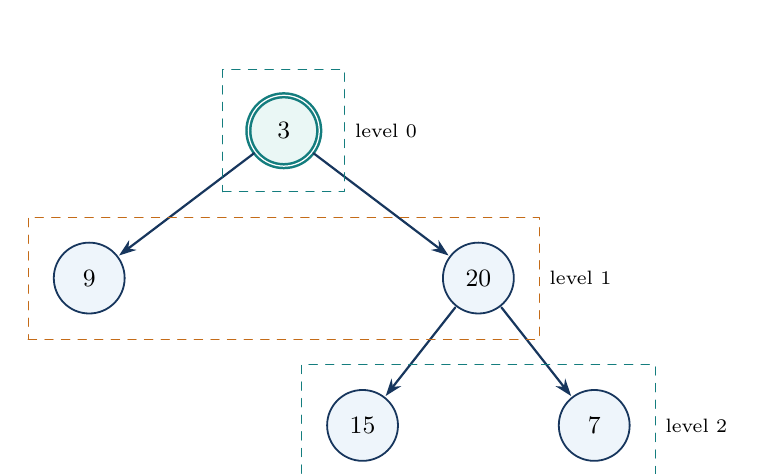
\begin{tikzpicture}[>={Stealth[length=2.2mm,width=1.55mm]},font=\small,level distance=12mm]
  \node[trienode,visited] (r) {3};
  \node[trienode,below left=12mm and 18mm of r] (a) {9};
  \node[trienode,below right=12mm and 18mm of r] (b) {20};
  \node[trienode,below left=12mm and 8mm of b] (c) {15};
  \node[trienode,below right=12mm and 8mm of b] (d) {7};
  \draw[flowarrow] (r)--(a); \draw[flowarrow] (r)--(b);
  \draw[flowarrow] (b)--(c); \draw[flowarrow] (b)--(d);
  \node[draw=teal,dashed,fit=(r),inner sep=3mm,label=right:{\scriptsize level 0}] {};
  \node[draw=orange,dashed,fit=(a)(b),inner sep=3mm,label=right:{\scriptsize level 1}] {};
  \node[draw=teal,dashed,fit=(c)(d),inner sep=3mm,label=right:{\scriptsize level 2}] {};
\end{tikzpicture}

\smallskip
Queue after each level: \texttt{[3]} $\rightarrow$ \texttt{[9,20]}
$\rightarrow$ \texttt{[15,7]}.
\end{visualbox}

\subsection{Algorithm and Key Idea}
Start by pushing the root. While the queue is not empty, save
\texttt{levelSize}, remove exactly that many nodes, append their values to one
row, and push each non-null child. The key rule is that every queued node is
unprocessed and the first \texttt{levelSize} nodes share the same depth.

\begin{invariantbox}{one saved queue prefix equals one tree level}
Immediately before an outer-loop round, the queue contains all unprocessed
nodes in breadth-first order. The saved size identifies exactly the current
depth; children appended during the round belong to the next depth and are
so not consumed until the following round.
\end{invariantbox}

\subsection{Pseudocode}
\begin{lstlisting}[style=pseudocode]
levelOrder(root):
    if root is null: return []
    queue = [root]
    result = []
    while queue is not empty:
        levelSize = queue.size()
        level = []
        repeat levelSize times:
            node = pop front
            append node.value to level
            push non-null children
        append level to result
    return result
\end{lstlisting}

\subsection{C++ Implementation}
\begin{lstlisting}[style=compactcode,caption={Complete C++ solution: Binary Tree Level Order Traversal}]
#include <queue>
#include <utility>
#include <vector>

using namespace std;

class Solution {
public:
    vector<vector<int>> levelOrder(TreeNode* root) {
        if (root == nullptr) return {};

        vector<vector<int>> result;
        queue<TreeNode*> pending;
        pending.push(root);

        while (!pending.empty()) {
            const int levelSize = static_cast<int>(pending.size());
            vector<int> level;
            level.reserve(levelSize);

            for (int i = 0; i < levelSize; ++i) {
                TreeNode* node = pending.front();
                pending.pop();
                level.push_back(node->val);
                if (node->left != nullptr) pending.push(node->left);
                if (node->right != nullptr) pending.push(node->right);
            }
            result.push_back(move(level));
        }
        return result;
    }
};
\end{lstlisting}

\subsection{Time, Space, and Common Mistakes}
Every node enters and leaves the queue once, so time is \(O(n)\). The queue
uses \(O(w)\) space, where \(w\) is the maximum tree width; the returned rows
use \(O(n)\) output space. Save the level size before pushing children, and
handle a null root before accessing it.

\begin{revisionbox}{How to explain it in an interview}
I use BFS because the output is grouped by depth. The queue contains the next
level. I snapshot its size, process exactly those nodes, and enqueue their
children for the following level. Each node is processed once: \(O(n)\) time
and \(O(w)\) extra queue space.
\end{revisionbox}

\subsection{Detailed Visual Dry Run}
For the worked example, the queue changes by complete levels. Children are
added only after the current node is removed.

\begin{dryrunbox}{Queue trace for \texttt{[3,9,20,null,null,15,7]}}
\begin{center}
\begin{tabularx}{\linewidth}{@{}c c X c@{}}
\toprule
Round & Saved size & Nodes processed and children appended & Output \\
\midrule
1 & 1 & Remove 3; append 9 and 20 & \texttt{[[3]]} \\
2 & 2 & Remove 9; remove 20 and append 15 and 7 & \texttt{[[3],[9,20]]} \\
3 & 2 & Remove 15 and 7; neither has children & \texttt{[[3],[9,20],[15,7]]} \\
\bottomrule
\end{tabularx}
\end{center}
\end{dryrunbox}

\begin{visualbox}{What the queue holds after each level}
\centering
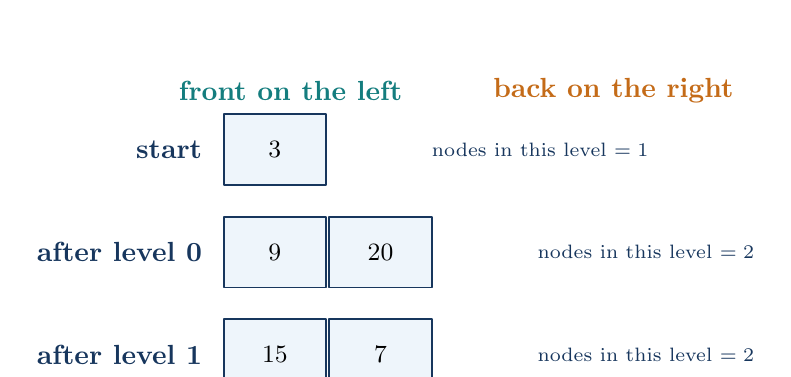
\begin{tikzpicture}[font=\small,>={Stealth[length=2.2mm,width=1.55mm]}]
  \node[text=teal,font=\bfseries] at (0.2,2.05) {front on the left};
  \node[text=orange,font=\bfseries] at (4.3,2.05) {back on the right};

  \node[text=navy,font=\bfseries,anchor=east] at (-0.8,1.3) {start};
  \node[arraycell,minimum width=13mm] (q0) at (0,1.3) {3};
  \node[right=12mm of q0,text=navy,font=\scriptsize] {nodes in this level \(=1\)};

  \node[text=navy,font=\bfseries,anchor=east] at (-0.8,0) {after level 0};
  \node[arraycell,minimum width=13mm] (q1) at (0,0) {9};
  \node[arraycell,minimum width=13mm,right=0mm of q1] (q2) {20};
  \node[right=12mm of q2,text=navy,font=\scriptsize] {nodes in this level \(=2\)};

  \node[text=navy,font=\bfseries,anchor=east] at (-0.8,-1.3) {after level 1};
  \node[arraycell,minimum width=13mm] (q3) at (0,-1.3) {15};
  \node[arraycell,minimum width=13mm,right=0mm of q3] (q4) {7};
  \node[right=12mm of q4,text=navy,font=\scriptsize] {nodes in this level \(=2\)};
\end{tikzpicture}
\end{visualbox}

The saved size is essential. If the loop instead continued until the queue
became empty, the children would be consumed in the same row as their parents
and the level grouping would be lost.

\subsection{Code Walkthrough}
\begin{enumerate}
  \item Reject a null root and return an empty result.
  \item Push the root into \texttt{pending}. The queue now represents the
  first unprocessed level.
  \item Copy \texttt{pending.size()} into \texttt{levelSize}. This value does
  not change when children are pushed later in the round.
  \item Pop exactly \texttt{levelSize} nodes, record their values, and enqueue
  their non-null children from left to right.
  \item Move the completed row into the result and repeat for the next depth.
\end{enumerate}

Although the code contains a loop inside another loop, it is still linear.
The inner loops across all rounds process each node exactly once; they do not
restart a full scan for every level.

\subsection{Edge Cases, Follow-ups, and Practice}
Test an empty tree, one node, a completely skewed tree, and a wide final
level. A common mistake is to enqueue null children and then dereference them.
Useful follow-ups include zigzag level order, returning only the rightmost
node at each depth, and computing the average value of every level.

\begin{revisionbox}{Practice checkpoint}
Without looking at the code, explain what the queue contains immediately
before each outer-loop iteration. Then modify the algorithm so alternating
rows are reversed while the traversal remains breadth first.
\end{revisionbox}
\chaptercheckpoint
  {The requested output is grouped by tree depth.}
  {A FIFO queue and the size of the current level.}
  {Processing newly enqueued children in the current output row.}
  {$O(n)$ time and $O(w)$ extra queue space.}
\judgeclassnote


\problemstart{Binary Tree Maximum Path Sum}{124}{Hard}{Postorder DFS}{Binary tree}

\subsection{The Problem}
A path may start and end at any nodes, but it cannot reuse a node. Return the
largest sum of any non-empty path. The path does not have to pass through the
root.

\begin{conceptbox}{Example}
For \texttt{[-10,9,20,null,null,15,7]}, the best path is
\(15\rightarrow20\rightarrow7\), so the answer is \(42\).
\end{conceptbox}

\subsection{Building the Recursive State}
A brute-force search could start a path at every node and explore many of the
same subtrees repeatedly. Postorder DFS removes that repetition. A parent can
continue through at most one child, so each recursive call returns the best
one-sided gain beginning at its node.

For a node with value \(x\): \(L=\max(0,\text{left gain}),\qquad R=\max(0,\text{right gain}).\)
The complete path turning at this node is \(L+x+R\). The value returned to the
parent is \(x+\max(L,R)\).

\begin{invariantbox}{a returned gain is always a single extendable chain}
After \texttt{gain(node)} finishes, its return value is the maximum sum of a
path that starts at \texttt{node} and travels downward through at most one
child. The global answer separately stores the best complete path seen so far,
which may use both children at exactly one turning node.
\end{invariantbox}

\begin{visualbox}{A path can join both children at one middle node}
\centering
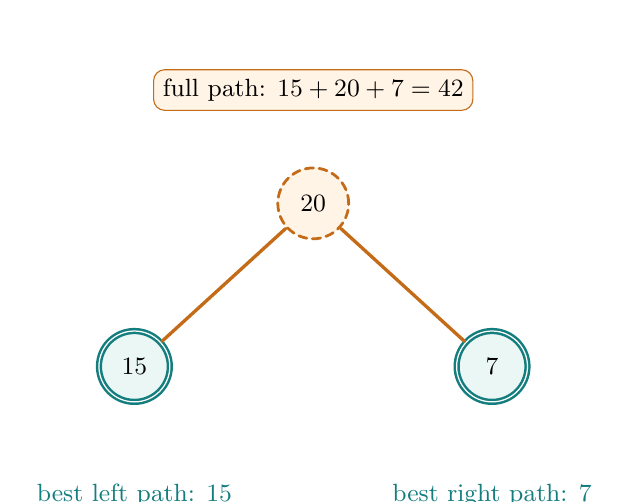
\begin{tikzpicture}[>={Stealth[length=2.2mm,width=1.55mm]},font=\small]
  \node[trienode,active] (r) {20};
  \node[trienode,visited,below left=14mm and 16mm of r] (l) {15};
  \node[trienode,visited,below right=14mm and 16mm of r] (q) {7};
  \draw[-,very thick,orange] (l)--(r)--(q);
  \node[below=9mm of l,text=teal] {best left path: 15};
  \node[below=9mm of q,text=teal] {best right path: 7};
  \node[above=7mm of r,draw=orange,fill=softorange,rounded corners]
    {full path: \(15+20+7=42\)};
\end{tikzpicture}
\end{visualbox}

\begin{visualbox}{A node sends only one branch up to its parent}
\centering
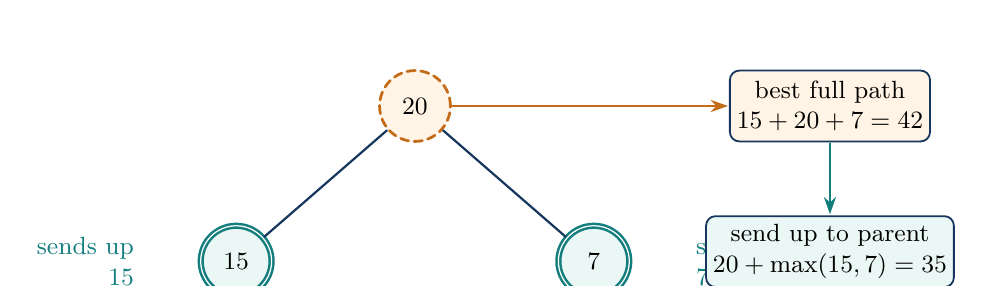
\begin{tikzpicture}[font=\small,>={Stealth[length=2.2mm,width=1.55mm]}]
  \node[trienode,active] (r) {20};
  \node[trienode,visited,below left=13mm and 16mm of r] (l) {15};
  \node[trienode,visited,below right=13mm and 16mm of r] (q) {7};
  \draw[-,thick,navy] (r)--(l) (r)--(q);
  \node[left=7mm of l,align=right,text=teal] {sends up\\15};
  \node[right=7mm of q,align=left,text=teal] {sends up\\7};
  \node[dsnode,right=35mm of r,fill=softorange] (full)
    {best full path\\\(15+20+7=42\)};
  \node[dsnode,below=9mm of full,fill=softteal] (up)
    {send up to parent\\\(20+\max(15,7)=35\)};
  \draw[flowarrow,orange] (r.east) -- (full.west);
  \draw[flowarrow,teal] (full) -- (up);
\end{tikzpicture}
\end{visualbox}

\subsection{Pseudocode}
\begin{lstlisting}[style=pseudocode]
dfs(node):
    if node is null: return 0
    leftGain = max(0, dfs(node.left))
    rightGain = max(0, dfs(node.right))
    answer = max(answer, leftGain + node.value + rightGain)
    return node.value + max(leftGain, rightGain)
\end{lstlisting}

\subsection{C++ Implementation}
\begin{lstlisting}[style=compactcode,caption={Complete C++ solution: Binary Tree Maximum Path Sum}]
#include <algorithm>
#include <limits>

using namespace std;

class Solution {
    int bestPath = numeric_limits<int>::min();

    int gain(TreeNode* node) {
        if (node == nullptr) return 0;
        const int left = max(0, gain(node->left));
        const int right = max(0, gain(node->right));
        bestPath = max(bestPath, node->val + left + right);
        return node->val + max(left, right);
    }

public:
    int maxPathSum(TreeNode* root) {
        bestPath = numeric_limits<int>::min();
        gain(root);
        return bestPath;
    }
};
\end{lstlisting}

\subsection{Why It Works and Complexity}
Postorder traversal makes both child gains available before processing the
parent. Every possible path has a highest turning node; the algorithm tests
that path when it processes that node. Negative gains are discarded because
they can only reduce the sum. Time is \(O(n)\), and recursion uses \(O(h)\)
stack space for tree height \(h\).

\begin{revisionbox}{Common mistakes}
Do not start the answer to zero because all node values may be negative.
Do not return the two-child path to the parent; that would branch and stop
being a valid path. Return only the better one-sided gain.
\end{revisionbox}

\begin{conceptbox}{All-negative tree}
For a tree such as \texttt{[-3,-2,-5]}, every child gain is clipped to zero,
but each node still tests its own value as a non-empty path. Initializing the
global answer to negative infinity returns \(-2\), while
initializing it to zero would incorrectly allow an empty path.
\end{conceptbox}

\subsection{From Brute Force to One Postorder Traversal}
A direct method could treat every node as a possible path start and explore
every possible continuation. Long chains and overlapping subtrees would then
be traversed repeatedly, leading to \(O(n^2)\) work on a skewed tree. The
optimized method asks each subtree one reusable question: ``What is the best
one-sided gain that can be extended through your parent?''

This returned value and the global answer are deliberately different:
\begin{itemize}
  \item the value returned upward may use at most one child;
  \item the complete choice recorded locally may join both child gains.
\end{itemize}

\subsection{Detailed Visual Dry Run}
\begin{dryrunbox}{Postorder values for \texttt{[-10,9,20,null,null,15,7]}}
\begin{center}
\begin{tabular}{@{}c c c c c@{}}
\toprule
Node & Left gain & Right gain & Complete choice & Gain returned \\
\midrule
9 & 0 & 0 & 9 & 9 \\
15 & 0 & 0 & 15 & 15 \\
7 & 0 & 0 & 7 & 7 \\
20 & 15 & 7 & 42 & 35 \\
-10 & 9 & 35 & 34 & 25 \\
\bottomrule
\end{tabular}
\end{center}
The best complete path is recorded at node 20. The value 42 is not returned to
node \(-10\), because returning both branches would create an invalid fork.
\end{dryrunbox}

\subsection{Code Walkthrough}
The helper first recurses left and right, so it is a postorder traversal.
\texttt{max(0, gain)} discards a negative branch. The expression
\texttt{node->val + left + right} tests the path whose highest turning point
is the current node. The helper then returns the current value plus only the
larger child gain. Resetting \texttt{bestPath} inside the public method makes
the same \texttt{Solution} object safe for another call.

\subsection{Edge Cases and Interview Follow-ups}
The tree may contain one negative node, all negative nodes, or a best path
that never touches the root. Recursion uses \(O(h)\) call-stack space and can
reach \(O(n)\) for a skewed tree. A useful follow-up is to return the actual
nodes in the maximum path; that requires storing or reconstructing the chosen
child direction as well as the sum.

\begin{revisionbox}{How to explain it simply}
Each recursive call returns the best downward path the parent can extend. At
each node I also test the complete path that joins the best non-negative left
and right gains. Every path has exactly one highest turning node, so one of
these local choices represents the global optimum.
\end{revisionbox}
\chaptercheckpoint
  {A path may begin and end anywhere, and a parent needs child results.}
  {One-sided postorder gains plus a global complete-path maximum.}
  {Returning the two-child choice upward or allowing an empty path.}
  {$O(n)$ time and $O(h)$ recursion space.}
\judgeclassnote


\patternintoc{Graph Traversal}
\problemstart{Clone Graph}{133}{Medium}{DFS with memoization}{Graph and hash map}

\subsection{The Problem}
Given one node in a connected undirected graph, return a deep copy. Every
original node must correspond to one new node, and neighbor relationships must
be keepd without sharing original pointers.

\subsection{Why a Hash Map Is Needed}
A plain recursive copy loops forever on cycles and may clone the same node more
than once. Store \(\text{original pointer}\rightarrow\text{clone pointer}\)
before recursing into neighbors. Seeing an existing key means the clone
is already available.

\begin{invariantbox}{every discovered original has exactly one registered clone}
Before DFS follows an outgoing edge, the current original node already has a
map entry. As a result, a back edge, self-loop, or shared neighbor always
returns the same clone pointer instead of allocating another object.
\end{invariantbox}

\begin{visualbox}{Copy every node and every connection}
\centering
\begin{tikzpicture}[>={Stealth[length=2.2mm,width=1.55mm]},font=\small]
  \node[trienode] (a) {1}; \node[trienode,right=16mm of a] (b) {2};
  \node[trienode,below=14mm of b] (c) {3}; \node[trienode,below=14mm of a] (d) {4};
  \draw[-,navy,thick] (a)--(b)--(c)--(d)--(a);
  \node[above=7mm of a,text=navy,font=\bfseries] {original};
  \node[right=18mm of b,font=\Large,text=teal] (arrow) {$\Longrightarrow$};
  \node[trienode,visited,right=18mm of arrow] (aa) {1'};
  \node[trienode,visited,right=16mm of aa] (bb) {2'};
  \node[trienode,visited,below=14mm of bb] (cc) {3'};
  \node[trienode,visited,below=14mm of aa] (dd) {4'};
  \draw[-,teal,thick] (aa)--(bb)--(cc)--(dd)--(aa);
  \node[above=7mm of aa,text=teal,font=\bfseries] {copy};
\end{tikzpicture}
\end{visualbox}

\subsection{Pseudocode}
\begin{lstlisting}[style=pseudocode]
clone(node):
    if node is null: return null
    if node is in cloneMap: return cloneMap[node]
    copy = new Node(node.value)
    cloneMap[node] = copy
    for neighbor in node.neighbors:
        copy.neighbors.push_back(clone(neighbor))
    return copy
\end{lstlisting}

\subsection{C++ Implementation}
\begin{lstlisting}[style=compactcode,caption={Complete C++ solution: Clone Graph}]
#include <unordered_map>

using namespace std;

class Solution {
    unordered_map<Node*, Node*> clones;

    Node* clone(Node* node) {
        if (node == nullptr) return nullptr;
        const auto found = clones.find(node);
        if (found != clones.end()) return found->second;

        Node* copy = new Node(node->val);
        clones[node] = copy;
        for (Node* neighbor : node->neighbors) {
            copy->neighbors.push_back(clone(neighbor));
        }
        return copy;
    }

public:
    Node* cloneGraph(Node* node) {
        clones.clear();
        return clone(node);
    }
};
\end{lstlisting}

\subsection{Why It Works, Time, and Space}
The map creates exactly one clone for every reachable original node. Each edge
is copied when its adjacency entry is visited. Time is \(O(V+E)\), map and
recursion space are \(O(V)\). Insert the clone into the map before visiting
neighbors; doing it afterward fails on cycles and self-loops.

\begin{revisionbox}{How to explain it in an interview}
I run DFS and memoize original-to-copy pointers. If a node was cloned already,
I reuse it. Otherwise I create and register the clone first, then recursively
copy every neighbor. This handles cycles and keeps shared neighbors.
\end{revisionbox}

\subsection{Why a Plain Recursive Copy Fails}
On a tree, recursively copying children eventually reaches null. A graph may
return to a node already on the active recursion path. Without the map, the
copy of node 1 asks for node 2, node 2 asks for node 1 again, and recursion
never ends. The map is both a cycle guard and the record that
keeps one-to-one node identity.

\subsection{Detailed Map and DFS Trace}
\begin{dryrunbox}{Cloning the four-node cycle}
\begin{center}
\begin{tabularx}{\linewidth}{@{}c X X@{}}
\toprule
Visit & Map before the recursive calls & Action \\
\midrule
1 & empty & create \(1'\), store \(1\to1'\), then visit its neighbors \\
2 & \(1\to1'\) & create \(2'\), store it, then visit neighbor 1 \\
1 again & \(1\to1',2\to2'\) & reuse \(1'\); do not recurse again \\
3 and 4 & earlier clones remain stored & create each once and copy every edge \\
\bottomrule
\end{tabularx}
\end{center}
\end{dryrunbox}

\begin{visualbox}{Each original node points to its one copy}
\centering
\begin{tikzpicture}[font=\small,>={Stealth[length=2.2mm,width=1.55mm]}]
  \node[dsnode,fill=softblue] (o1) {old node 1};
  \node[dsnode,below=7mm of o1,fill=softblue] (o2) {old node 2};
  \node[dsnode,below=7mm of o2,fill=softblue] (o3) {old node 3};
  \node[dsnode,right=38mm of o1,fill=softteal] (c1) {copy \(1'\)};
  \node[dsnode,below=7mm of c1,fill=softteal] (c2) {copy \(2'\)};
  \node[dsnode,below=7mm of c2,fill=softteal] (c3) {copy \(3'\)};
  \draw[flowarrow,teal] (o1)--node[edgelabel,above,font=\scriptsize]{saved pair} (c1);
  \draw[flowarrow,teal] (o2)--(c2);
  \draw[flowarrow,teal] (o3)--(c3);
  \node[draw=navy,dashed,fit=(o1)(o2)(o3)(c1)(c2)(c3),inner sep=5mm,
    label=above:{\small\textbf{saved old-to-copy pairs}}] {};
\end{tikzpicture}

\smallskip
If an old node appears again, the saved pair returns the same copy. This keeps
all shared connections and cycles correct.
\end{visualbox}

\begin{visualbox}{If a node was copied already, stop going deeper}
\centering
\begin{tikzpicture}[font=\small,>={Stealth[length=2.2mm,width=1.55mm]}]
  \node[draw=navy,fill=softblue,minimum width=43mm,minimum height=8mm] (g0)
    {copy node 1};
  \node[draw=navy,fill=softblue,minimum width=43mm,minimum height=8mm,
    above=0mm of g0] (g1) {copy node 2};
  \node[draw=orange,fill=softorange,minimum width=43mm,minimum height=8mm,
    above=0mm of g1] (g2) {see node 1 again};
  \node[left=12mm of g2,text=orange,font=\bfseries,align=right] (top) {working\\now};
  \draw[flowarrow,orange] (top)--(g2);
  \node[dsnode,right=25mm of g1,fill=softteal] (hit)
    {node 1 already has copy \(1'\)\\use that copy};
  \draw[flowarrow,teal] (g2.east)--(hit.north west);
\end{tikzpicture}

\smallskip
The repeated node creates nothing new. Use its saved copy and finish this
function call.
\end{visualbox}

\subsection{Code Walkthrough}
\begin{enumerate}
  \item A null input represents an empty graph and returns null.
  \item Search \texttt{clones} before allocating. An existing entry means the
  node and all references to its identity already have a copy.
  \item Allocate a new node and immediately place it in the map.
  \item Recursively clone every neighbor and append the returned pointer to
  the copy's adjacency vector in the same order.
\end{enumerate}

The immediate insertion in step 3 is the key rule-preserving step. It makes
the partial clone visible before an edge can lead back to it.

\subsection{Edge Cases, Alternative, and Practice}
Test a single isolated node, a self-loop, two nodes connected to each other,
and several nodes sharing the same neighbor. Verify that cloned pointers are
different from all original pointers. An iterative BFS alternative uses a
queue plus the same original-to-clone map and has the same \(O(V+E)\) cost.

\begin{revisionbox}{Practice checkpoint}
Draw a graph containing a self-loop and explain exactly why registering the
copy after cloning its neighbors would recurse forever.
\end{revisionbox}
\chaptercheckpoint
  {A pointer-based graph must be copied without sharing original objects.}
  {An original-pointer-to-clone-pointer hash map and DFS stack.}
  {Registering a clone only after recursively visiting its neighbors.}
  {$O(V+E)$ time and $O(V)$ map plus traversal space.}
\judgeclassnote


\patternintoc{Dynamic Programming}
\problemstart{Coin Change}{322}{Medium}{Bottom-up dynamic programming}{One-dimensional DP}

\subsection{The Problem}
Given coin denominations and a target amount, return the fewest coins needed
to form that amount. Coins may be reused. Return \(-1\) when the amount is
unreachable.

\begin{conceptbox}{Example}
With \texttt{coins=[1,2,5]} and \texttt{amount=11}, the best construction is
\(5+5+1\), so the answer is \(3\).
\end{conceptbox}

\subsection{How We Get to the Solution}
Trying every sequence of coins creates an exponential recursion tree. The same
remaining amounts occur repeatedly. Let \(dp[x]\) be the minimum number of
coins needed to form \(x\). Start \(dp[0]=0\) and every other entry to an
unreachable sentinel \(\texttt{amount}+1\).

For each amount \(x\) and each coin \(c\le x\): \(dp[x]=\min(dp[x],1+dp[x-c]).\)

\begin{invariantbox}{every smaller amount is already best}
When the outer loop reaches amount \(x\), each referenced state \(dp[x-c]\)
has already been finalized. Trying every possible final coin tests
every construction of \(x\), and the minimum choice becomes best.
\end{invariantbox}

\begin{visualbox}{To make 11, add coin 5 to the best answer for 6}
\centering
\begin{tikzpicture}[font=\small]
  \foreach \x/\v in {0/0,1/1,2/1,3/2,4/2,5/1,6/2,7/2,8/3,9/3,10/2,11/3} {
    \node[arraycell] (d\x) at (0.8*\x,0) {\v};
    \node[below=1mm of d\x,font=\scriptsize] {\x};
  }
  \draw[flowarrow,orange] (d6.north) to[bend left=28]
    node[edgelabel,above,font=\scriptsize]{add coin 5} (d11.north);
\end{tikzpicture}
\end{visualbox}

\subsection{Pseudocode}
\begin{lstlisting}[style=pseudocode]
dp = array(amount + 1, amount + 1)
dp[0] = 0
for current from 1 through amount:
    for coin in coins:
        if coin <= current:
            dp[current] = min(dp[current], 1 + dp[current - coin])
return -1 if dp[amount] is unreachable, otherwise dp[amount]
\end{lstlisting}

\subsection{C++ Implementation}
\begin{lstlisting}[style=compactcode,caption={Complete C++ solution: Coin Change}]
#include <algorithm>
#include <vector>

using namespace std;

class Solution {
public:
    int coinChange(vector<int>& coins, int amount) {
        vector<int> dp(amount + 1, amount + 1);
        dp[0] = 0;

        for (int current = 1; current <= amount; ++current) {
            for (const int coin : coins) {
                if (coin <= current) {
                    dp[current] = min(dp[current], 1 + dp[current - coin]);
                }
            }
        }
        return dp[amount] == amount + 1 ? -1 : dp[amount];
    }
};
\end{lstlisting}

\subsection{Time and Space}
For \(A=\texttt{amount}\) and \(m\) coin types, time is \(O(A m)\) and space
is \(O(A)\). The key rule is that before computing \(dp[x]\), every smaller
amount is already best. Avoid using zero as the default for unreachable
amounts; it would look like a free solution.

\begin{revisionbox}{Pattern clue}
When a target can be built from reusable choices and the question asks for a
minimum, maximum, or count, define the answer for every smaller target and
extend those solved states.
\end{revisionbox}

\subsection{Brute Force and Repeated Work}
A recursive brute-force solution tries every coin, subtracts it from the
remaining amount, and repeats. For amount 11, branches such as
\(11\to10\to8\) and \(11\to9\to8\) both solve the same remaining amount 8.
Without memoization, the recursion tree grows exponentially. The DP table
stores the answer to each remaining amount once.

\subsection{Detailed Table Walkthrough}
\begin{dryrunbox}{Building \(dp\) for coins \texttt{[1,2,5]}}
\begin{center}
\begin{tabularx}{\linewidth}{@{}c c X@{}}
\toprule
Amount & Best count & Reason \\
\midrule
0 & 0 & base case: no coins are needed \\
1 & 1 & \(1+dp[0]\) using coin 1 \\
2 & 1 & coin 2 is better than two coin-1 choices \\
5 & 1 & one coin of value 5 \\
6 & 2 & coin 1 plus the best answer for 5 \\
10 & 2 & \(5+5\) \\
11 & 3 & \(1+dp[10]\), producing \(1+5+5\) \\
\bottomrule
\end{tabularx}
\end{center}
\end{dryrunbox}

The sentinel \texttt{amount + 1} is safe because no valid answer can require
more than \texttt{amount} positive-valued coins when coin 1 exists. More
generally, it simply represents a value worse than every possible valid
answer under the problem rules.

\subsection{Code Walkthrough}
The outer loop grows the solved prefix from 1 through \texttt{amount}. For
each coin not larger than the current amount, the code considers taking that
coin last. The remaining state \texttt{current - coin} is smaller and has
already been solved. After all coins are tested, \texttt{dp[current]} is the
minimum among every possible final coin.

\subsection{Edge Cases, Alternatives, and Interview Notes}
Amount zero returns zero. An empty coin list or unreachable amount returns
\(-1\). Duplicate denominations do not change the minimum but perform
unneeded work. A top-down memoized solution uses the same update rule and
is valuable when only a small subset of amounts is reached.

For example, \texttt{coins=[2]} and \texttt{amount=3} leaves \(dp[3]\) at the
sentinel because neither amount 1 nor amount 3 can be formed. This is different
from a valid answer of zero, which occurs only when the requested amount is
zero.

\begin{revisionbox}{How to explain it simply}
I define \(dp[x]\) as the fewest coins needed for amount \(x\). For every
amount, I try each denomination as the final coin and extend the already
best state \(dp[x-c]\). The table prevents repeated recursion and gives
\(O(A m)\) time with \(O(A)\) space.
\end{revisionbox}
\chaptercheckpoint
  {Reusable choices build a target and the objective asks for a minimum.}
  {A DP entry for the minimum coins required by every smaller amount.}
  {Using zero for unreachable states or forgetting the amount-zero base case.}
  {$O(A m)$ time and $O(A)$ space.}
\judgeclassnote


\problemstart{Combination Sum IV}{377}{Medium}{Ordered-count dynamic programming}{One-dimensional DP}

\subsection{The Problem}
Given distinct positive integers and a target, count the ordered sequences that
sum to the target. With \texttt{nums=[1,2,3]} and target \(4\), the answer is
\(7\). For example, \([1,3]\) and \([3,1]\) are different combinations.

\subsection{Reasoning and Loop Order}
Let \(dp[x]\) be the number of ordered sequences totaling \(x\). The empty
sequence is one way to create zero, so \(dp[0]=1\). For every target value
from \(1\) upward, try every number as the final element: \(dp[x] = \sum_{v\le x} dp[x-v].\)
The outer loop must be the current total and the inner loop the choice
number. Reversing them counts unordered coin combinations instead.

\begin{invariantbox}{the table counts every ordered sequence by its final value}
Before computing \(dp[x]\), all counts for smaller totals are complete. The
sequences ending with different final values do not overlap, so adding
\(dp[x-v]\) over every valid \(v\) counts each ordered sequence exactly once.
\end{invariantbox}

\begin{visualbox}{Three last-number choices build the answer for 4}
\centering
\begin{tikzpicture}[font=\small,>={Stealth[length=2.2mm,width=1.55mm]}]
  \node[dsnode,visited] (one) at (0,1.35) {last number 1\\4 ways to make 3};
  \node[dsnode] (two) at (0,0) {last number 2\\2 ways to make 2};
  \node[dsnode,fill=softorange] (three) at (0,-1.35) {last number 3\\1 way to make 1};
  \node[dsnode,active,minimum width=27mm] (answer) at (4.8,0)
    {total ways for 4\\\(4+2+1=7\)};
  \draw[flowarrow,teal] (one.east)--(answer.north west);
  \draw[flowarrow,navy] (two.east)--(answer.west);
  \draw[flowarrow,orange] (three.east)--(answer.south west);
  \foreach \x/\v in {0/1,1/1,2/2,3/4,4/7} {
    \node[arraycell,minimum width=11mm] (dp\x) at ({1.1+1.3*\x},-2.75) {\v};
    \node[below=1mm of dp\x,font=\scriptsize] {\(dp[\x]\)};
  }
  \node[draw=orange,very thick,fit=(dp4),inner sep=1mm] {};
\end{tikzpicture}

\smallskip
For total 4, group the sequences by their last number. The three groups contain
4, 2, and 1 sequence, giving \(4+2+1=7\).
\end{visualbox}

\begin{dryrunbox}{DP for \texttt{[1,2,3]} and target 4}
\begin{center}
\begin{tabular}{c|ccccc}
Target \(x\) & 0 & 1 & 2 & 3 & 4 \\ \hline
\(dp[x]\) & 1 & 1 & 2 & 4 & 7
\end{tabular}
\end{center}
\end{dryrunbox}

\subsection{Pseudocode and C++ Implementation}
\begin{lstlisting}[style=pseudocode]
dp[0] = 1
for total from 1 through target:
    for value in nums:
        if value <= total:
            dp[total] += dp[total - value]
return dp[target]
\end{lstlisting}

\begin{lstlisting}[style=compactcode,caption={Complete C++ solution: Combination Sum IV}]
#include <vector>

using namespace std;

class Solution {
public:
    int combinationSum4(vector<int>& nums, int target) {
        vector<unsigned long long> dp(target + 1, 0);
        dp[0] = 1;
        for (int total = 1; total <= target; ++total) {
            for (const int value : nums) {
                if (value <= total) dp[total] += dp[total - value];
            }
        }
        return static_cast<int>(dp[target]);
    }
};
\end{lstlisting}

\subsection{Why It Works, Complexity, and Common Mistakes}
Every valid sequence totaling \(x\) has one final value \(v\); removing it
leaves a sequence counted by \(dp[x-v]\). These groups do not overlap, so their
counts add exactly. Time is \(O(Tm)\), space is \(O(T)\), where \(T\) is the
target and \(m\) is the number of values. Do not set \(dp[0]=0\), and remember
that order matters in this problem.

\begin{revisionbox}{How to explain it in an interview}
I count ways for every smaller total. The base \(dp[0]=1\) represents choosing
nothing. For each total, I try each number as the last choice and add the ways
to form the remaining total. This produces ordered sequences in \(O(Tm)\).
\end{revisionbox}

\subsection{Why the Loop Order Counts Ordered Sequences}
The worked example contains seven sequences for target 4. The important detail is
that \([1,3]\) and \([3,1]\) are different. The outer loop chooses
the total being built, while the inner loop tries every possible final value.
For each final value, all prefixes that form the remaining total are appended
with that value.

If the loops were reversed---numbers outside and totals inside---the table
would count unordered coin combinations instead. Loop order is part of the
meaning of the state, not merely a coding preference.

\subsection{Complete Dry Run}
\begin{dryrunbox}{Seven sequences for target 4}
\begin{center}
\begin{tabular}{@{}c c l@{}}
\toprule
Total & Ways & Sequences added by their last value \\
\midrule
0 & 1 & empty prefix \\
1 & 1 & \([1]\) \\
2 & 2 & \([1,1],[2]\) \\
3 & 4 & \([1,1,1],[2,1],[1,2],[3]\) \\
4 & 7 & \([1,1,1,1],[2,1,1],[1,2,1],[3,1],\) \\
  &   & \([1,1,2],[2,2],[1,3]\) \\
\bottomrule
\end{tabular}
\end{center}
\end{dryrunbox}

\subsection{Code Walkthrough and Safety}
The unsigned table provides extra intermediate range, while the problem
guarantees the final answer fits a signed 32-bit integer. The base value 1 at
index zero represents the one valid empty prefix. Every access uses
\texttt{total - value} only after confirming that the result is non-negative.

\subsection{Edge Cases and Follow-ups}
Target zero has one empty sequence. A number greater than the target is simply
ignored. Inputs must be positive; allowing zero or negative values would
break the increasing-state dependency and could create infinitely many
sequences. A common follow-up asks for unordered combinations, which requires
reversing the loop order.

\begin{revisionbox}{Practice checkpoint}
Explain why \(dp[0]\) is one even though the answer contains no number. Then
rewrite the update rule for combinations where order does not matter.
\end{revisionbox}
\chaptercheckpoint
  {The problem counts ordered ways to reach a target.}
  {A DP count for each total, beginning with the empty sequence at zero.}
  {Reversing the loops and accidentally counting unordered combinations.}
  {$O(Tm)$ time and $O(T)$ space.}
\judgeclassnote


\patternintoc{Tree Construction}
\problemstart{Construct Binary Tree from Preorder and Inorder Traversal}{105}{Medium}{Recursive partitioning}{Tree and hash map}

\subsection{The Problem}
Preorder lists each root before its subtrees. Inorder lists the left subtree,
then the root, then the right subtree. Reconstruct and return the unique tree
when all values are distinct.

\begin{conceptbox}{Example}
\texttt{preorder=[3,9,20,15,7]} and
\texttt{inorder=[9,3,15,20,7]} reconstruct the tree rooted at \(3\), with
left child \(9\) and right subtree rooted at \(20\).
\end{conceptbox}

\subsection{Recursive Split}
The next unused preorder value is the current root. Its position in inorder
splits the current interval into left and right subtrees. A hash map gives that
position in average \(O(1)\) time, avoiding a repeated linear search.

\begin{invariantbox}{the next preorder value roots the current inorder interval}
Each recursive call owns exactly one consecutive inorder interval. The shared
preorder index points to that interval's root; after the left call consumes
all left-subtree nodes, the right call begins at exactly the next unused
preorder value.
\end{invariantbox}

\begin{visualbox}{Preorder gives the root; inorder shows its left and right sides}
\centering
\begin{tikzpicture}[font=\small]
  \node[dsnode,fill=softorange] (pre) {preorder\\\texttt{3 | 9 | 20 15 7}};
  \node[dsnode,below=10mm of pre] (in) {inorder\\\texttt{9 | 3 | 15 20 7}};
  \draw[flowarrow,orange] (pre.south)--node[edgelabel,right,font=\scriptsize]{root 3} (in.north);
  \node[below left=9mm and 13mm of in,text=teal] {left side: \texttt{[9]}};
  \node[below right=9mm and 13mm of in,text=navy] {right side: \texttt{[15,20,7]}};
\end{tikzpicture}
\end{visualbox}

\begin{visualbox}{The map finds each root; the stack remembers unfinished ranges}
\centering
\begin{tikzpicture}[font=\small,>={Stealth[length=2.2mm,width=1.55mm]}]
  \node[dsnode,align=left,fill=softteal] (map) {
    \textbf{position of each value}\\
    \(9\to0\)\quad \(3\to1\)\\
    \(15\to2\)\quad \(20\to3\)\\
    \(7\to4\)};
  \node[draw=navy,fill=softblue,minimum width=46mm,minimum height=8mm,
    right=28mm of map] (b0) {whole range: root 3};
  \node[draw=navy,fill=softblue,minimum width=46mm,minimum height=8mm,
    above=0mm of b0] (b1) {left range: root 9};
  \node[draw=orange,fill=softorange,minimum width=46mm,minimum height=8mm,
    above=0mm of b1] (b2) {empty range: stop};
  \node[above=5mm of map,text=teal,font=\bfseries] {find the root quickly};
  \node[right=7mm of b2,text=orange,font=\bfseries,align=left] {working\\now};
  \draw[flowarrow,teal] (map.east)--node[edgelabel,above,font=\scriptsize]{root position} (b0.west);
\end{tikzpicture}

\smallskip
The map tells us where the root sits. The stack remembers which left and right
parts still need to be built.
\end{visualbox}

\subsection{Pseudocode}
\begin{lstlisting}[style=pseudocode]
build(left, right):
    if left > right: return null
    rootValue = preorder[preorderIndex++]
    root = new TreeNode(rootValue)
    middle = inorderPosition[rootValue]
    root.left = build(left, middle - 1)
    root.right = build(middle + 1, right)
    return root
\end{lstlisting}

\subsection{C++ Implementation}
\begin{lstlisting}[style=compactcode,caption={Complete C++ solution: Construct Binary Tree}]
#include <unordered_map>
#include <vector>

using namespace std;

class Solution {
    const vector<int>* preorderValues = nullptr;
    unordered_map<int, int> inorderIndex;
    int preorderIndex = 0;

    TreeNode* build(int left, int right) {
        if (left > right) return nullptr;
        const int rootValue = (*preorderValues)[preorderIndex++];
        TreeNode* root = new TreeNode(rootValue);
        const int middle = inorderIndex[rootValue];
        root->left = build(left, middle - 1);
        root->right = build(middle + 1, right);
        return root;
    }

public:
    TreeNode* buildTree(vector<int>& preorder, vector<int>& inorder) {
        preorderValues = &preorder;
        preorderIndex = 0;
        inorderIndex.clear();
        for (int i = 0; i < static_cast<int>(inorder.size()); ++i) {
            inorderIndex[inorder[i]] = i;
        }
        return build(0, static_cast<int>(inorder.size()) - 1);
    }
};
\end{lstlisting}
\judgeclassnote

\subsection{Why It Works, Time, and Space}
Each call consumes exactly one preorder root and assigns it the inorder range
that contains exactly its descendants. Building the left range before the
right range matches preorder order. Every node is created once, so time and
stored map space are \(O(n)\); recursion uses \(O(h)\) stack space.

\begin{revisionbox}{Common mistakes}
Build the left subtree before the right subtree because preorder lists the
entire left subtree first. Use interval boundaries instead of copying array
slices. The distinct-value assumption is what makes the inorder index unique.
\end{revisionbox}

\subsection{Direct Method and Its Limitation}
A simple recursive version can search the full inorder array for every new
root. It constructs the correct tree, but the repeated linear searches cost
\(O(n^2)\) for a skewed tree. Building a value-to-index map once changes every
root lookup to average \(O(1)\), producing an \(O(n)\) construction.

\subsection{Detailed Recursive Walkthrough}
\begin{dryrunbox}{Preorder \texttt{[3,9,20,15,7]}, inorder \texttt{[9,3,15,20,7]}}
\begin{center}
\begin{tabularx}{\linewidth}{@{}c c c X@{}}
\toprule
Call & Next preorder root & Inorder interval & Result \\
\midrule
1 & 3 & \([0,4]\) & split at index 1; left \([0,0]\), right \([2,4]\) \\
2 & 9 & \([0,0]\) & leaf; both child intervals are empty \\
3 & 20 & \([2,4]\) & split at index 3 \\
4 & 15 & \([2,2]\) & left leaf of 20 \\
5 & 7 & \([4,4]\) & right leaf of 20 \\
\bottomrule
\end{tabularx}
\end{center}
\end{dryrunbox}

\begin{visualbox}{The tree after all left and right parts are built}
\centering
\begin{tikzpicture}[font=\small,>={Stealth[length=2.2mm,width=1.55mm]}]
  \node[trienode,active] (r) {3};
  \node[trienode,below left=13mm and 22mm of r] (n9) {9};
  \node[trienode,below right=13mm and 22mm of r] (n20) {20};
  \node[trienode,visited,below left=13mm and 9mm of n20] (n15) {15};
  \node[trienode,visited,below right=13mm and 9mm of n20] (n7) {7};
  \draw[flowarrow] (r)--node[edgelabel,above left,font=\scriptsize]{left side} (n9);
  \draw[flowarrow] (r)--node[edgelabel,above right,font=\scriptsize]{right side} (n20);
  \draw[flowarrow] (n20)--(n15); \draw[flowarrow] (n20)--(n7);
  \node[below=5mm of n9,font=\scriptsize,text=teal]{position 0};
  \node[below=5mm of n15,font=\scriptsize,text=teal]{position 2};
  \node[below=5mm of n7,font=\scriptsize,text=teal]{position 4};
\end{tikzpicture}
\end{visualbox}

The preorder pointer advances exactly once per created node. The inorder
boundaries determine when a subtree is empty; no array slices need to be
allocated.

\subsection{Code Walkthrough}
The public method stores a pointer to the preorder vector, resets the shared
index, and creates the inorder lookup map. The helper reads the next root,
allocates it, finds its inorder position, and recursively builds the left
interval before the right interval. The base case \texttt{left > right}
returns a null child.

\subsection{Assumptions, Edge Cases, and Follow-ups}
The traversals must contain the same distinct values and represent a valid
tree. Empty arrays produce a null root. A skewed tree uses \(O(n)\) recursion
depth. Duplicate values make the reconstruction ambiguous unless extra
occurrence information is supplied. A useful variation reconstructs from
inorder and postorder; in that case roots are consumed from the end and the
right subtree must be built first.

\begin{revisionbox}{How to explain it simply}
Preorder tells me the next root. Its position in inorder divides the exact
left and right descendant ranges. A hash map removes repeated searches, and a
single preorder index ensures each node is consumed once, for \(O(n)\) time.
\end{revisionbox}
\chaptercheckpoint
  {Two traversals reveal roots and subtree boundaries in complementary orders.}
  {A preorder cursor, inorder index map, and recursive interval boundaries.}
  {Building the right subtree first or copying slices at every call.}
  {$O(n)$ time, $O(n)$ map space, and $O(h)$ recursion space.}
% Additional lessons: arrays, bits, graphs, lists, and strings.

\patternintoc{Two Pointers}
\problemstart{Container With Most Water}{11}{Medium}{Two pointers}{Array}

\subsection{The Problem}
Each array value is the height of a vertical line. Choose two lines that form
the container with the greatest area. For indexes \(l<r\): \(\text{area}=\min(h_l,h_r)(r-l).\)

\begin{conceptbox}{Example}
For \texttt{[1,8,6,2,5,4,8,3,7]}, lines at indexes \(1\) and \(8\) create
area \(\min(8,7)\cdot7=49\).
\end{conceptbox}

\subsection{From Brute Force to Two Pointers}
Checking every pair takes \(O(n^2)\). Start with the widest possible pair.
The shorter line limits the area. Moving the taller line inward only reduces
width while keeping the same limiting height or worse, so it cannot improve
that pair. Move the shorter line and search for a taller boundary.

\begin{invariantbox}{every removed wall is safely dominated}
Before each iteration, every pair outside the current interval has already
been measured or proved unable to beat a measured pair. Once the current area
is recorded, any narrower pair that keeps the shorter wall has no greater
limiting height, so that wall may be discarded.
\end{invariantbox}

\begin{visualbox}{The shorter wall limits how much water fits}
\centering
\begin{tikzpicture}[>={Stealth[length=2.2mm,width=1.55mm]},font=\small,x=8mm,y=4mm]
  \foreach \x/\h in {0/1,1/8,2/6,3/2,4/5,5/4,6/8,7/3,8/7} {
    \draw[navy,very thick] (\x,0)--(\x,\h);
    \node[below] at (\x,0) {\scriptsize \x};
  }
  \begin{scope}[on background layer]
    \fill[softteal,opacity=.65] (1,0) rectangle (8,7);
  \end{scope}
  \draw[teal,very thick] (1,0)--(1,8); \draw[orange,very thick] (8,0)--(8,7);
  \node[above=2mm,text=teal,font=\bfseries] at (1,8) {left: 8};
  \node[above=2mm,text=orange,font=\bfseries] at (8,7) {right: 7};
  \draw[decorate,decoration={brace,amplitude=4pt},navy]
    (1,-1.1)--(8,-1.1) node[midway,below=4mm]{width \(=7\)};
  \node[fill=white,rounded corners,inner sep=2mm] at (4.5,3.5)
    {area \(=7\times7=49\)};
\end{tikzpicture}
\end{visualbox}

\subsection{Pseudocode and C++ Implementation}
\begin{lstlisting}[style=pseudocode]
left = 0, right = n - 1, best = 0
while left < right:
    best = max(best, min(height[left], height[right]) * (right-left))
    if height[left] <= height[right]: left++
    else: right--
return best
\end{lstlisting}

\begin{lstlisting}[style=compactcode,caption={Complete C++ solution: Container With Most Water}]
#include <algorithm>
#include <vector>

using namespace std;

class Solution {
public:
    int maxArea(vector<int>& height) {
        int left = 0;
        int right = static_cast<int>(height.size()) - 1;
        long long best = 0;

        while (left < right) {
            const long long width = right - left;
            const long long wall = min(height[left], height[right]);
            best = max(best, width * wall);
            if (height[left] <= height[right]) ++left;
            else --right;
        }
        return static_cast<int>(best);
    }
};
\end{lstlisting}

\subsection{Why It Works, Time, and Space}
When a pair is processed, every pair that keeps its shorter wall and uses a
smaller width is no better. Discarding that wall cannot remove the best
unseen pair. Each pointer moves at most \(n-1\) times, so time is \(O(n)\) and
space is \(O(1)\).

\begin{revisionbox}{Common mistake}
Area uses the smaller height, not the larger one. This is not binary search:
the pointers move according to which boundary limits the current container.
\end{revisionbox}

\subsection{Detailed Pointer Dry Run}
\begin{dryrunbox}{Worked example \texttt{[1,8,6,2,5,4,8,3,7]}}
\begin{center}
\begin{tabularx}{\linewidth}{@{}c c c c X@{}}
\toprule
Left, right & Heights & Width & Area & Pointer removed \\
\midrule
0, 8 & 1, 7 & 8 & 8 & left: height 1 limits the pair \\
1, 8 & 8, 7 & 7 & 49 & right: height 7 is shorter \\
1, 7 & 8, 3 & 6 & 18 & right \\
1, 6 & 8, 8 & 5 & 40 & either equal wall may move \\
2, 6 & 6, 8 & 4 & 24 & left \\
\bottomrule
\end{tabularx}
\end{center}
No later pair exceeds 49, so the answer is the container between indexes 1
and 8.
\end{dryrunbox}

\subsection{Why Moving the Shorter Wall Is Safe}
Suppose the left wall is shorter. Keeping it while moving the right pointer
inward reduces the width and cannot increase the limiting height above that
same left wall. Every such pair is no better than the current pair. The only
chance to improve is to discard the shorter wall and search for a taller one.
This reason is the key rule behind the two-pointer method.

\subsection{Code Walkthrough}
The code begins with the widest possible pair. It calculates width and the
smaller boundary with \texttt{long long} intermediates, updates the best area,
and advances exactly one pointer. Since every iteration shrinks the interval,
the loop terminates after at most \(n-1\) moves.

\subsection{Edge Cases and Follow-ups}
Two lines form the smallest valid input. Zero-height lines are allowed and
simply create zero area. Equal boundary heights may move either side because
the current limiting height cannot improve while the width shrinks. A common
follow-up asks why sorting is impossible: the original index distance is part
of the area and must be keepd.

\begin{revisionbox}{How to explain it simply}
I start with maximum width. The shorter wall limits the current area, and any
narrower pair that keeps that wall cannot do better. I move the
shorter side, test each remaining choice once, and obtain \(O(n)\) time and
\(O(1)\) space.
\end{revisionbox}
\chaptercheckpoint
  {Two boundaries determine an area, and moving inward always reduces width.}
  {Left and right pointers plus the best area seen so far.}
  {Moving the taller wall without proving which boundary is safely discardable.}
  {$O(n)$ time and $O(1)$ extra space.}
\judgeclassnote


\patternintoc{Arrays, Hashing, and Bits}
\problemstart{Contains Duplicate}{217}{Easy}{Membership hashing}{Hash set}

\subsection{The Problem}
Return true when any integer appears at least twice. Return false when every
value is distinct.

\subsection{How We Get to the Solution}
Comparing every pair costs \(O(n^2)\). Sorting costs \(O(n\log n)\) and changes
the input order. A hash set answers the exact question we need: have we seen
this value before?

\begin{invariantbox}{the set equals the distinct processed prefix}
Immediately before reading \texttt{nums[i]}, the set contains every distinct
value at an earlier index and no future value. A membership hit is a
real duplicate; otherwise insertion keeps the statement for the next
iteration.
\end{invariantbox}

\begin{visualbox}{Stop when a number appears again}
\centering
\begin{tikzpicture}[>={Stealth[length=2.2mm,width=1.55mm]},font=\small]
  \foreach \x/\v in {0/1,1/2,2/3,3/1} {
    \node[arraycell] (a\x) at (1.2*\x,0) {\v};
  }
  \node[dsnode,right=22mm of a3] (s) {numbers already seen\\\{1,2,3\}};
  \draw[flowarrow,orange] (a3)--node[edgelabel,above,font=\scriptsize]{seen 1 before} (s);
  \node[below=7mm of s,draw=orange,fill=softorange,rounded corners] {duplicate found};
\end{tikzpicture}
\end{visualbox}

\subsection{Pseudocode}
\begin{lstlisting}[style=pseudocode]
seen = empty set
for value in nums:
    if value is already in seen: return true
    insert value into seen
return false
\end{lstlisting}

\subsection{C++ Implementation}
\begin{lstlisting}[style=compactcode,caption={Complete C++ solution: Contains Duplicate}]
#include <unordered_set>
#include <vector>

using namespace std;

class Solution {
public:
    bool containsDuplicate(vector<int>& nums) {
        unordered_set<int> seen;
        seen.reserve(nums.size());
        for (const int value : nums) {
            if (!seen.insert(value).second) return true;
        }
        return false;
    }
};
\end{lstlisting}

\subsection{Complexity and Revision}
Hash insertion is average-case \(O(1)\), giving average \(O(n)\) time and
\(O(n)\) space. The worst-case hash bound is \(O(n^2)\), although interview
analysis normally states the average case. Empty and one-element arrays return
false.

\begin{revisionbox}{Pattern clue}
Questions asking whether an item has appeared before usually suggest a set.
Questions needing information attached to that item suggest a map.
\end{revisionbox}

\subsection{Example Walkthrough}
For \texttt{[1,2,3,1]}, the set evolves as follows:
\begin{dryrunbox}{Insertion result reveals the duplicate}
\begin{center}
\begin{tabular}{@{}c c c@{}}
\toprule
Current value & Set before insertion & Result \\
\midrule
1 & \(\{\}\) & insert succeeds \\
2 & \(\{1\}\) & insert succeeds \\
3 & \(\{1,2\}\) & insert succeeds \\
1 & \(\{1,2,3\}\) & insert fails; return true \\
\bottomrule
\end{tabular}
\end{center}
\end{dryrunbox}

The set is enough because only membership matters. A map would store an
unneeded second value.

\subsection{Code Walkthrough and Alternatives}
\texttt{seen.reserve(nums.size())} reduces avoidable rehashing but is not
required for why the solution works. \texttt{insert} returns a pair whose Boolean field
is false when the key already exists, allowing lookup and insertion in one
operation. Returning immediately avoids scanning the rest of the array.

Sorting is an alternative: sort, then compare adjacent values in
\(O(n\log n)\) time and constant or implementation-dependent extra space.
The nested-loop baseline uses \(O(1)\) space but \(O(n^2)\) time.

\subsection{Edge Cases and Interview Notes}
Empty and one-element inputs are distinct by definition. Negative values and
zero require no special handling. Repeated values may appear more than twice;
the second occurrence is enough. Hash operations are average-case constant
time, not a deterministic worst-case guarantee.

\begin{revisionbox}{Practice checkpoint}
Change the question to ``return the first duplicated value'' and explain why
the same scan works. Then change it to ``return each value's frequency'' and
identify why a map is now required.
\end{revisionbox}
\chaptercheckpoint
  {The question asks whether a value has appeared earlier.}
  {A hash set containing the distinct processed values.}
  {Forgetting that hash bounds are average case or using a map when only membership matters.}
  {$O(n)$ average time and $O(n)$ space.}
\judgeclassnote


\problemstart{Counting Bits}{338}{Easy}{Bit dynamic programming}{Array}

\subsection{The Problem}
For every integer from \(0\) through \(n\), return the number of set bits in
its binary representation. For \(n=5\), return \texttt{[0,1,1,2,1,2]}.

\subsection{Update Rule}
Counting every number bit by bit takes \(O(n\log n)\). Dividing \(i\) by two
removes its last binary digit, and \(i\&1\) tells us whether that removed digit
was one: \(bits[i]=bits[i\!>>\!1]+(i\&1).\)

\begin{invariantbox}{the shifted dependency is already solved}
When the loop reaches \(i\), the index \(i>>1\) is smaller than \(i\), so its
bit count is already correct. Adding the removed least-significant bit gives
the exact count for \(i\) and extends the solved prefix by one entry.
\end{invariantbox}

\begin{visualbox}{Use the answer for 2 to find the answer for 5}
\centering
\begin{tikzpicture}[font=\small,>={Stealth[length=2.2mm,width=1.55mm]},node distance=10mm]
  \node[dsnode,active] (five) {\(5=101_2\)};
  \node[dsnode,right=of five] (shift) {remove last digit\\\(101\to10\)};
  \node[dsnode,right=of shift,visited] (known) {ones in 2\\\(=1\)};
  \node[dsnode,below=12mm of shift,fill=softorange] (last) {removed digit\\is 1};
  \node[dsnode,right=14mm of last,active] (answer) {ones in 5\\\(=2\)};
  \draw[flowarrow] (five)--(shift);
  \draw[flowarrow] (shift)--(known);
  \draw[flowarrow,teal] (known.south) to[bend right=18] (answer.north);
  \draw[flowarrow,orange] (last)--(answer);
  \foreach \x/\v in {0/0,1/1,2/1,3/2,4/1,5/2} {
    \node[arraycell,minimum width=10mm] (bit\x) at ({-0.2+1.12*\x},-3.35) {\v};
    \node[below=1mm of bit\x,font=\scriptsize] {\x};
  }
  \node[left=8mm of bit0,text=navy,font=\bfseries,align=right] {answers for\\0 through 5};
  \node[draw=orange,very thick,fit=(bit5),inner sep=1mm] {};
\end{tikzpicture}
\end{visualbox}

\begin{dryrunbox}{Binary update rule}
\begin{center}
\begin{tabular}{c|cccccc}
\(i\) & 0 & 1 & 2 & 3 & 4 & 5 \\ \hline
binary & 0 & 1 & 10 & 11 & 100 & 101 \\
set bits & 0 & 1 & 1 & 2 & 1 & 2
\end{tabular}
\end{center}
\end{dryrunbox}

\subsection{Pseudocode}
\begin{lstlisting}[style=pseudocode]
bits[0] = 0
for value from 1 through n:
    bits[value] = bits[value / 2] + (value mod 2)
return bits
\end{lstlisting}

\subsection{C++ Implementation}
\begin{lstlisting}[style=compactcode,caption={Complete C++ solution: Counting Bits}]
#include <vector>

using namespace std;

class Solution {
public:
    vector<int> countBits(int n) {
        vector<int> bits(n + 1, 0);
        for (int value = 1; value <= n; ++value) {
            bits[value] = bits[value >> 1] + (value & 1);
        }
        return bits;
    }
};
\end{lstlisting}

\subsection{Why It Works and Complexity}
The update rule reuses the already-computed answer for \(\lfloor i/2\rfloor\)
and adds the final bit. Time is \(O(n)\); extra working space is \(O(1)\)
excluding the required \(O(n)\) output. The base \(bits[0]=0\) is essential.

\subsection{Building the Bit Update Rule}
Every non-negative integer \(i\) can be written as \(i=2\left\lfloor i/2\right\rfloor +(i\bmod 2).\)
Shifting right removes the final bit. The expression \texttt{i \& 1} is one
for an odd number and zero for an even number. So the number of set
bits is the answer for the shifted value plus the removed bit.

\begin{dryrunbox}{Binary states from 0 through 5}
\begin{center}
\begin{tabular}{@{}c c c c c@{}}
\toprule
\(i\) & Binary & \(i>>1\) & Final bit & \(bits[i]\) \\
\midrule
0 & 000 & -- & -- & 0 \\
1 & 001 & 0 & 1 & \(bits[0]+1=1\) \\
2 & 010 & 1 & 0 & \(bits[1]+0=1\) \\
3 & 011 & 1 & 1 & \(bits[1]+1=2\) \\
4 & 100 & 2 & 0 & \(bits[2]+0=1\) \\
5 & 101 & 2 & 1 & \(bits[2]+1=2\) \\
\bottomrule
\end{tabular}
\end{center}
\end{dryrunbox}

\subsection{Code Explanation, Alternatives, and Edge Cases}
The output vector is filled with zeros, so the base case is already
present. The loop starts at one; \texttt{value >> 1} is always smaller and
has already been computed. A direct method could count bits separately for
every integer in \(O(n\log n)\). Another useful update rule is
\(bits[i]=bits[i\&(i-1)]+1\), which removes the lowest set bit.

For \(n=0\), the output is \texttt{[0]}. The vector is required output space,
so it should not be described as avoidable extra memory.

\begin{revisionbox}{How to explain it in an interview}
I reuse the count for the number with its final binary digit removed. Right
shift gives that smaller number, and \texttt{i \& 1} tells whether the removed
digit contributes one. Each answer is built in constant time, so the entire
range takes \(O(n)\).
\end{revisionbox}
\chaptercheckpoint
  {Each number reduces to a smaller number whose answer is known.}
  {The required output array of bit counts from zero through $n$.}
  {Recounting every binary representation independently.}
  {$O(n)$ time and $O(n)$ required output storage.}
\judgeclassnote


\patternintoc{Directed Graphs}
\problemstart{Course Schedule}{207}{Medium}{DFS cycle detection}{Directed graph}

\subsection{The Problem}
Courses are vertices. A prerequisite pair \([a,b]\) means \(b\rightarrow a\):
course \(b\) must be completed before \(a\). Return whether every course can
be finished.

\subsection{Key Observation}
A valid schedule exists exactly when the prerequisite graph has no directed
cycle. The three-state method tracks both fully visited nodes and nodes in the current DFS
path. A three-state array expresses the same idea:
\begin{itemize}
  \item \(0\): unvisited,
  \item \(1\): visiting in the current recursion path,
  \item \(2\): completely processed and safe.
\end{itemize}

\begin{invariantbox}{state 1 is exactly the active DFS path}
A course changes from unvisited to visiting when its DFS frame begins and
changes to done only after all outgoing edges are proved safe. So an
edge to state 1 is a back edge and a cycle, whereas an edge to state 2 can be
reused without more recursion.
\end{invariantbox}

\begin{visualbox}{Following the arrows returns to course 0}
\centering
\begin{tikzpicture}[>={Stealth[length=2.2mm,width=1.55mm]},font=\small,node distance=18mm]
  \node[trienode,active] (a) {0};
  \node[trienode,active,right=of a] (b) {1};
  \node[trienode,active,right=of b] (c) {2};
  \draw[flowarrow,orange] (a)--(b); \draw[flowarrow,orange] (b)--(c);
  \draw[flowarrow,orange] (c) to[bend left=35] node[edgelabel,above]{returns to active course} (a);
\end{tikzpicture}
\end{visualbox}

\subsection{Pseudocode}
\begin{lstlisting}[style=pseudocode]
hasCycle(course):
    if state[course] == visiting: return true
    if state[course] == done: return false
    state[course] = visiting
    for next in graph[course]:
        if hasCycle(next): return true
    state[course] = done
    return false
\end{lstlisting}

\subsection{C++ Implementation}
\begin{lstlisting}[style=compactcode,caption={Complete C++ solution: Course Schedule}]
#include <vector>

using namespace std;

class Solution {
    bool hasCycle(int course,
                  const vector<vector<int>>& graph,
                  vector<int>& state) {
        if (state[course] == 1) return true;
        if (state[course] == 2) return false;
        state[course] = 1;
        for (const int next : graph[course]) {
            if (hasCycle(next, graph, state)) return true;
        }
        state[course] = 2;
        return false;
    }

public:
    bool canFinish(int numCourses,
                   vector<vector<int>>& prerequisites) {
        vector<vector<int>> graph(numCourses);
        for (const auto& edge : prerequisites) graph[edge[1]].push_back(edge[0]);
        vector<int> state(numCourses, 0);
        for (int course = 0; course < numCourses; ++course) {
            if (hasCycle(course, graph, state)) return false;
        }
        return true;
    }
};
\end{lstlisting}

\subsection{Why It Works, Time, and Space}
A visiting neighbor is an ancestor in the current DFS path, so that edge closes
a directed cycle. Done nodes have already been proved cycle-free and need not
be explored again. Time and storage are \(O(V+E)\); recursion depth is
\(O(V)\) in the worst case.

\begin{revisionbox}{How to explain it in an interview}
I build the prerequisite graph and run DFS from every course. A three-state
array distinguishes an active recursion path from a completed node. Reaching
an active node proves a cycle, so the courses cannot all be finished.
\end{revisionbox}

\subsection{Why One Visited Boolean Is Not Enough}
A node seen in a different completed DFS branch is safe; a node seen again in
the current recursion path proves a cycle. A single Boolean cannot distinguish
those situations. The three states mean unvisited, visiting, and completely
processed. Only an edge to a visiting node is a back edge.

\subsection{Detailed DFS Trace}
\begin{dryrunbox}{Cycle in prerequisites \texttt{[[1,0],[0,1]]}}
\begin{center}
\begin{tabularx}{\linewidth}{@{}c c X@{}}
\toprule
Action & States \((0,1)\) & Meaning \\
\midrule
Enter course 0 & \((1,0)\) & 0 is on the active path \\
Follow \(0\to1\) & \((1,1)\) & 1 joins the active path \\
Follow \(1\to0\) & \((1,1)\) & 0 is already visiting; cycle found \\
\bottomrule
\end{tabularx}
\end{center}
For \texttt{[[1,0]]}, course 1 finishes, changes to state 2, and no back edge
is found.
\end{dryrunbox}

\begin{visualbox}{Three labels separate new, active, and finished courses}
\centering
\begin{tikzpicture}[font=\small,>={Stealth[length=2.2mm,width=1.55mm]}]
  \node[trienode,active] (c0) {0};
  \node[trienode,active,right=18mm of c0] (c1) {1};
  \draw[flowarrow,orange] (c0) to[bend left=18] (c1);
  \draw[flowarrow,orange] (c1) to[bend left=18] (c0);

  \node[right=32mm of c1,text=navy,font=\bfseries] (label) {course labels};
  \node[arraycell,active,below=5mm of label,xshift=-8mm] (s0) {1};
  \node[arraycell,active,right=5mm of s0] (s1) {1};
  \node[below=2mm of s0,font=\scriptsize] {course 0};
  \node[below=2mm of s1,font=\scriptsize] {course 1};
  \node[below=14mm of s0,anchor=north west,xshift=-2mm,
    align=left,font=\scriptsize,text=navy] {
    0 = not started\\1 = being checked now\\2 = finished and safe};
\end{tikzpicture}

\smallskip
An arrow to a course labeled 1 returns to the path being checked, so there is
a cycle.
\end{visualbox}

\begin{visualbox}{Course arrows and the path being checked}
\centering
\begin{tikzpicture}[font=\small,>={Stealth[length=2.2mm,width=1.55mm]}]
  \node[dsnode,align=left,fill=softteal] (adj) {
    \textbf{next course}\\
    \texttt{0: [1]}\\
    \texttt{1: [0]}};
  \node[draw=navy,fill=softblue,minimum width=44mm,minimum height=8mm,
    right=30mm of adj] (f0) {check course 0};
  \node[draw=navy,fill=softblue,minimum width=44mm,minimum height=8mm,
    above=0mm of f0] (f1) {check course 1};
  \node[draw=orange,fill=softorange,minimum width=44mm,minimum height=8mm,
    above=0mm of f1] (f2) {see course 0 again};
  \node[right=7mm of f2,text=orange,font=\bfseries,align=left] {working\\now};
  \draw[flowarrow,teal] (adj.east)--node[edgelabel,above,font=\scriptsize]{follow arrow} (f0.west);
  \node[below=8mm of f0,draw=orange,fill=softorange,rounded corners,
    font=\scriptsize] {course 0 is already on this path \(\Rightarrow\) cycle};
\end{tikzpicture}
\end{visualbox}

\subsection{Code Walkthrough}
The adjacency list stores edges from each prerequisite to the course unlocked
by it. The helper returns immediately for visiting and done states. Before
exploring neighbors it marks the course visiting; after every neighbor is
proved safe, it marks the course done. The outer loop is needed because
the graph may contain several disconnected components.

\subsection{Alternative, Edge Cases, and Follow-ups}
Kahn's topological-sort algorithm is an equally strong alternative: repeatedly
take zero-indegree courses and check whether all courses are removed. An empty
prerequisite list is immediately possible. A self-dependency such as
\([0,0]\) is a cycle. Duplicate edges do not change the DFS result, though
they add repeated adjacency work.

\begin{visualbox}{Two methods notice the same impossible loop}
\centering
\begin{tikzpicture}[font=\small,>={Stealth[length=2.2mm,width=1.55mm]}]
  \node[dsnode,fill=softorange] (dfs) {path view\\returns to an active course};
  \node[dsnode,right=24mm of dfs,fill=softteal] (kahn)
    {ready-list view\\no course is ready};
  \node[dsnode,below=12mm of $(dfs)!0.5!(kahn)$] (blocked)
    {the loop leaves no valid next course};
  \draw[flowarrow,orange] (dfs)--(blocked);
  \draw[flowarrow,teal] (kahn)--(blocked);
\end{tikzpicture}
\end{visualbox}

\begin{revisionbox}{Practice checkpoint}
Modify the solution to return one valid course order. Decide whether DFS
postorder or Kahn's queue makes that extension easier to explain.
\end{revisionbox}
\chaptercheckpoint
  {Prerequisites form directed dependencies that must admit an ordering.}
  {An adjacency list and three DFS states, or indegrees and a queue.}
  {Treating every previously visited node as a cycle instead of only active nodes.}
  {$O(V+E)$ time and $O(V+E)$ graph/traversal space.}
\judgeclassnote


\patternintoc{String DP}
\problemstart{Decode Ways}{91}{Medium}{Prefix dynamic programming}{String and DP}

\subsection{The Problem}
Digits map from \(1\) through \(26\) to letters. Count the ways to split a digit
string into valid codes. A zero cannot be decoded by itself.

\begin{conceptbox}{Examples}
\texttt{"12"} has two decodings: \texttt{1|2} and \texttt{12}.
\texttt{"226"} has three. \texttt{"06"} has zero because a code cannot start
with zero.
\end{conceptbox}

\subsection{DP State}
Let \(dp[i]\) be the number of decodings for the first \(i\) characters.
Start \(dp[0]=1\) for the empty prefix. At position \(i\):
\begin{itemize}
  \item if the one-digit code is \(1\) through \(9\), add \(dp[i-1]\);
  \item if the two-digit code is \(10\) through \(26\), add \(dp[i-2]\).
\end{itemize}

\begin{invariantbox}{each prefix count contains every valid ending once}
After processing length \(i\), \(dp[i]\) counts exactly the decodings of the
first \(i\) characters. Every decoding ends with either one nonzero digit or
one valid value from 10 through 26, so the previous groups are complete
and do not overlap.
\end{invariantbox}

\begin{visualbox}{For \texttt{226}, count endings \texttt{6} and \texttt{26}}
\centering
\begin{tikzpicture}[font=\small,>={Stealth[length=2.2mm,width=1.55mm]}]
  \node[arraycell,minimum width=12mm] (s0) {2};
  \node[arraycell,minimum width=12mm,right=0mm of s0] (s1) {2};
  \node[arraycell,minimum width=12mm,right=0mm of s1,active] (s2) {6};
  \node[below=2mm of s0,font=\scriptsize] {1};
  \node[below=2mm of s1,font=\scriptsize] {2};
  \node[below=2mm of s2,font=\scriptsize] {3};

  \node[dsnode,above=15mm of s1,xshift=-10mm] (one) {end with \texttt{6}\\2 earlier ways};
  \node[dsnode,above=15mm of s2,xshift=14mm,fill=softorange] (two) {end with \texttt{26}\\1 earlier way};
  \node[dsnode,right=20mm of s2,active] (ways) {total\\\(2+1=3\)};
  \draw[flowarrow,teal] (one)--(ways.north west);
  \draw[flowarrow,orange] (two)--(ways.north);
  \foreach \x/\v in {0/1,1/1,2/2,3/3} {
    \node[arraycell,minimum width=11mm] (decode\x) at ({0.1+1.25*\x},-1.55) {\v};
    \node[below=1mm of decode\x,font=\scriptsize] {\(dp[\x]\)};
  }
  \node[left=8mm of decode0,text=navy,font=\bfseries,align=right] {ways after\\each prefix};
  \node[draw=orange,very thick,fit=(decode3),inner sep=1mm] {};
\end{tikzpicture}

\smallskip
Every decoding ends with either \texttt{6} or \texttt{26}. These are separate
groups, so their counts are added.
\end{visualbox}

\begin{dryrunbox}{Decoding \texttt{"226"}}
\begin{center}
\begin{tabular}{c|cccc}
Prefix length & 0 & 1 & 2 & 3 \\ \hline
Prefix & empty & 2 & 22 & 226 \\
Ways & 1 & 1 & 2 & 3
\end{tabular}
\end{center}
\end{dryrunbox}

\subsection{Pseudocode}
\begin{lstlisting}[style=pseudocode]
if text is empty or starts with 0: return 0
dp[0] = 1
dp[1] = 1
for prefixLength from 2 through text.length:
    if last digit is 1 through 9:
        dp[prefixLength] += dp[prefixLength - 1]
    if last two digits form 10 through 26:
        dp[prefixLength] += dp[prefixLength - 2]
return dp[text.length]
\end{lstlisting}

\subsection{C++ Implementation}
\begin{lstlisting}[style=compactcode,caption={Complete C++ solution: Decode Ways}]
#include <string>
#include <vector>

using namespace std;

class Solution {
public:
    int numDecodings(string s) {
        if (s.empty() || s[0] == '0') return 0;
        const int n = static_cast<int>(s.size());
        vector<int> dp(n + 1, 0);
        dp[0] = 1;
        dp[1] = 1;

        for (int i = 2; i <= n; ++i) {
            if (s[i - 1] != '0') dp[i] += dp[i - 1];
            const int twoDigits = (s[i - 2] - '0') * 10 + (s[i - 1] - '0');
            if (twoDigits >= 10 && twoDigits <= 26) dp[i] += dp[i - 2];
        }
        return dp[n];
    }
};
\end{lstlisting}

\subsection{Why It Works, Complexity, and Common Mistakes}
Every valid decoding ends in exactly one valid one-digit or two-digit code, so
the update rule splits all possibilities without overlap. Time and space
are \(O(n)\). Carefully reject standalone zero, values above 26, and prefixes
such as \texttt{"06"}. The DP can be reduced to \(O(1)\) space because only
the previous two entries are needed.

\subsection{Brute Force and Repeated Prefixes}
A recursive solution may decode one digit, decode two digits when valid, and
recurse on the remaining suffix. For a string of many ones, both branches are
available repeatedly and the recursion grows exponentially. The same suffix
or prefix length is solved many times. Dynamic programming stores the number
of decodings for each prefix exactly once.

\subsection{Detailed Prefix Dry Run}
\begin{dryrunbox}{Decoding \texttt{"226"}}
\begin{center}
\begin{tabularx}{\linewidth}{@{}c c c X@{}}
\toprule
Prefix & One-digit choice & Two-digit choice & Ways \\
\midrule
empty & -- & -- & \(dp[0]=1\) \\
\texttt{2} & \texttt{2} is valid & -- & \(dp[1]=1\) \\
\texttt{22} & append \texttt{2}: \(dp[1]\) & append \texttt{22}: \(dp[0]\) & 2 \\
\texttt{226} & append \texttt{6}: \(dp[2]\) & append \texttt{26}: \(dp[1]\) & 3 \\
\bottomrule
\end{tabularx}
\end{center}
The three decodings are \texttt{2|2|6}, \texttt{22|6}, and
\texttt{2|26}.
\end{dryrunbox}

\subsection{Code Walkthrough}
The first-character guard rejects an empty input or leading zero. The table
uses prefix lengths, so \texttt{dp[i]} describes the first \(i\) characters.
If the last character is nonzero, every decoding of the previous prefix can
append it. If the last two characters form 10 through 26, every decoding two
positions back can append that pair.

\subsection{Important Zero Cases and Follow-ups}
\texttt{"10"} and \texttt{"20"} each have one decoding. \texttt{"30"},
\texttt{"06"}, and \texttt{"100"} are invalid. The pair test must require at
least 10, not merely at most 26. Since only two earlier states are read, the
table can be compressed to two integers for \(O(1)\) extra space.

\begin{dryrunbox}{Zero-heavy strings that expose invalid transitions}
\begin{center}
\begin{tabularx}{\linewidth}{@{}c c X@{}}
\toprule
String & Ways & Reason \\
\midrule
\texttt{0} & 0 & zero cannot stand alone \\
\texttt{10} & 1 & only the pair 10 is valid \\
\texttt{101} & 1 & \texttt{10|1}; zero blocks the one-digit transition \\
\texttt{100} & 0 & the final zero cannot pair with zero \\
\texttt{226} & 3 & \texttt{2|2|6}, \texttt{22|6}, and \texttt{2|26} \\
\bottomrule
\end{tabularx}
\end{center}
\end{dryrunbox}

\begin{revisionbox}{How to explain it simply}
Every decoding ends with either one valid digit or one valid two-digit code.
Those two groups do not overlap, so I add the matching prefix counts. The
DP scans once in \(O(n)\) time and explicitly handles zeros.
\end{revisionbox}
\chaptercheckpoint
  {A prefix can end with one-character or two-character codes.}
  {The number of valid decodings for each processed prefix.}
  {Allowing zero alone or accepting a two-digit number outside 10--26.}
  {$O(n)$ time and $O(n)$ space, reducible to $O(1)$.}
\judgeclassnote


\patternintoc{Linked Lists}
\problemstart{Linked List Cycle}{141}{Easy}{Floyd's two-pointer cycle detection}{Linked list}

\subsection{The Problem}
Return whether repeatedly following \texttt{next} can revisit a node. The
platform's cycle position is not passed to the function.

\subsection{Why Slow and Fast Pointers Meet}
A hash set can store visited pointers in \(O(n)\) space. Floyd's algorithm uses
two pointers: slow advances one edge and fast advances two. If there is no
cycle, fast reaches null. Inside a cycle, fast gains one node per iteration on
slow and must eventually meet it.

\begin{invariantbox}{null proves an end; pointer equality proves repetition}
After \(k\) rounds, slow has moved \(k\) edges and fast has moved \(2k\). If
fast reaches null, the list is finite. If both pointers reference the same
node, different traversal distances have reached one object, which can happen
only after entering a cycle.
\end{invariantbox}

\begin{visualbox}{Fast catches slow when the list loops}
\centering
\begin{tikzpicture}[>={Stealth[length=2.2mm,width=1.55mm]},font=\small,node distance=14mm]
  \node[trienode] (a) {3}; \node[trienode,right=of a] (b) {2};
  \node[trienode,right=of b] (c) {0}; \node[trienode,right=of c] (d) {-4};
  \draw[flowarrow] (a)--(b)--(c)--(d);
  \draw[flowarrow,orange] (d) to[bend right=45] node[edgelabel,below]{loop back} (b);
  \node[above=7mm of b,text=teal] {slow};
  \node[above=7mm of c,text=orange] {fast};
\end{tikzpicture}
\end{visualbox}

\subsection{Pseudocode}
\begin{lstlisting}[style=pseudocode]
slow = head
fast = head
while fast exists and fast.next exists:
    slow = slow.next
    fast = fast.next.next
    if slow equals fast: return true
return false
\end{lstlisting}

\subsection{C++ Implementation}
\begin{lstlisting}[style=compactcode,caption={Complete C++ solution: Linked List Cycle}]
using namespace std;

class Solution {
public:
    bool hasCycle(ListNode* head) {
        ListNode* slow = head;
        ListNode* fast = head;
        while (fast != nullptr && fast->next != nullptr) {
            slow = slow->next;
            fast = fast->next->next;
            if (slow == fast) return true;
        }
        return false;
    }
};
\end{lstlisting}

\subsection{Time and Space}
Both pointers make \(O(n)\) total progress before fast reaches null or the
pointers meet. Extra space is \(O(1)\). Check both \texttt{fast} and
\texttt{fast->next} before advancing two steps.

\begin{revisionbox}{Pattern clue}
Use slow and fast pointers when repeated next-state transitions may enter a
cycle and the problem asks for constant extra space.
\end{revisionbox}

\subsection{From a Hash Set to Constant Space}
The simplest solution stores every visited node pointer in a hash set. Before
advancing, it checks whether the current pointer was seen before. This is
linear time and linear space. Floyd's method removes the set by using two
walkers with different speeds.

If a cycle exists, slow and fast eventually enter it. After that, fast gains
one node on slow per iteration, measured around the cycle. The distance
modulo the cycle length must eventually become zero, so the pointers meet.

\subsection{Pointer Dry Run}
\begin{dryrunbox}{List \(3\to2\to0\to-4\), with \(-4\to2\)}
\begin{center}
\begin{tabular}{@{}c c c@{}}
\toprule
Iteration & Slow & Fast \\
\midrule
start & 3 & 3 \\
1 & 2 & 0 \\
2 & 0 & 2 \\
3 & -4 & -4 \\
\bottomrule
\end{tabular}
\end{center}
The equal pointers refer to the same node object, not merely equal stored
values. So a repeated value in an acyclic list does not create a false
cycle.
\end{dryrunbox}

\begin{visualbox}{Without a loop, fast reaches the end}
\centering
\begin{tikzpicture}[font=\small,>={Stealth[length=2.2mm,width=1.55mm]}]
  \node[dsnode] (a) {1}; \node[dsnode,right=10mm of a] (b) {2};
  \node[dsnode,right=10mm of b] (c) {3}; \node[dsnode,right=10mm of c] (d) {4};
  \node[right=10mm of d] (null) {end};
  \draw[flowarrow] (a)--(b)--(c)--(d)--(null);
  \node[above=7mm of b,text=teal,font=\bfseries] {slow};
  \node[above=7mm of d,text=orange,font=\bfseries] {fast};
  \node[below=8mm of d,text=navy] {fast reaches the end \(\Rightarrow\) no loop};
\end{tikzpicture}
\end{visualbox}

\subsection{Code Explanation and Safety}
Both pointers begin at the head. The loop verifies that fast and
\texttt{fast->next} exist before moving fast two edges. The comparison occurs
after movement; if a cycle exists, the pointers eventually become identical.
If fast reaches null, the list has a finite end.

\subsection{Edge Cases and Interview Follow-ups}
Test an empty list, one node without a loop, one node pointing to itself, a
two-node cycle, and a long non-cyclic prefix before a short cycle. A common
follow-up asks for the cycle's entry node: after the first meeting, reset one
pointer to head and advance both one step at a time; their next meeting is the
entry.

\begin{revisionbox}{Practice checkpoint}
Explain why comparing \texttt{slow->val == fast->val} is incorrect. Then
derive how resetting one pointer after the meeting locates the cycle entry.
\end{revisionbox}
\chaptercheckpoint
  {Repeated next-pointer transitions may enter a cycle.}
  {Slow and fast node pointers.}
  {Comparing values instead of pointer identity or dereferencing past null.}
  {$O(n)$ time and $O(1)$ extra space.}
\judgeclassnote


\patternintoc{String Design}
\problemstart{Encode and Decode Strings}{271}{Medium}{Length-prefixed encoding}{Strings}

\subsection{The Problem}
Design two operations: encode a vector of arbitrary strings into one string,
then decode it back exactly. Strings may be empty and may contain delimiter
characters.

\subsection{Why a Delimiter Alone Fails}
Joining with \texttt{\#} is ambiguous when a payload itself contains
\texttt{\#}. Prefix every string with its decimal length and a delimiter: \(\boxed{\texttt{length\#payload}}.\)
The decoder reads the length first, so it knows exactly how many following
characters belong to the payload.

\begin{invariantbox}{the cursor always begins at the next frame length}
After decoding a frame, the cursor has advanced past its decimal length, the
separator, and exactly the announced payload characters. Separators inside a
payload are never interpreted, so the next cursor position is clear.
\end{invariantbox}

\begin{visualbox}{Each stored string says its own length}
\centering
\begin{tikzpicture}[font=\small]
  \node[dsnode] (a) {\texttt{4\#lint}};
  \node[dsnode,right=4mm of a] (b) {\texttt{4\#code}};
  \node[dsnode,right=4mm of b] (c) {\texttt{0\#}};
  \node[dsnode,right=4mm of c] (d) {\texttt{3\#a\#b}};
  \node[below=7mm of $(a)!0.5!(d)$] {the number says how many characters come next};
\end{tikzpicture}
\end{visualbox}

\subsection{Pseudocode}
\begin{lstlisting}[style=pseudocode]
encode(strings): append length + '#' + string for every string
decode(data):
    i = 0
    while i < data.length:
        find next '#'
        parse length before it
        copy exactly length characters after it
        advance i to the next frame
\end{lstlisting}

\subsection{C++ Implementation}
\begin{lstlisting}[style=compactcode,caption={Complete C++ solution: Encode and Decode Strings}]
#include <string>
#include <vector>

using namespace std;

class Codec {
public:
    string encode(const vector<string>& strings) {
        string encoded;
        for (const string& value : strings) {
            encoded += to_string(value.size());
            encoded.push_back('#');
            encoded += value;
        }
        return encoded;
    }

    vector<string> decode(const string& encoded) {
        vector<string> result;
        size_t index = 0;
        while (index < encoded.size()) {
            const size_t delimiter = encoded.find('#', index);
            const size_t length =
                static_cast<size_t>(stoull(encoded.substr(index, delimiter-index)));
            const size_t start = delimiter + 1;
            result.push_back(encoded.substr(start, length));
            index = start + length;
        }
        return result;
    }
};
\end{lstlisting}

\subsection{Why It Works, Complexity, and Edge Cases}
Every frame has one clear numeric prefix. The decoder consumes exactly
the announced payload length, even when the payload contains \texttt{\#} or is
empty. Encoding and decoding both take \(O(N)\) time for total character count
\(N\), with \(O(N)\) returned storage. Test empty vectors, empty strings,
delimiter characters, and multi-digit lengths.

\begin{revisionbox}{How to explain it in an interview}
I avoid delimiter ambiguity by storing the payload length before each string.
The decoder finds the separator, parses the length, copies exactly that many
characters, and continues at the next frame.
\end{revisionbox}

\subsection{Why Simple Joining Is Not Reversible}
Suppose the separator is \texttt{\#}. Encoding
\texttt{["ab","c\#d"]} as \texttt{ab\#c\#d} loses the information that the
second separator belongs inside a payload. Escaping separators is possible,
but then the escape character itself must also be escaped. A length prefix is
simpler because payload contents no longer affect parsing.

\subsection{Frame-by-Frame Dry Run}
\begin{dryrunbox}{Encoding \texttt{["lint","code","","a\#b"]}}
\begin{center}
\begin{tabular}{@{}c c c@{}}
\toprule
String & Frame & Decoder action \\
\midrule
\texttt{lint} & \texttt{4\#lint} & read 4, then copy four characters \\
\texttt{code} & \texttt{4\#code} & read 4, then copy four characters \\
empty & \texttt{0\#} & read 0 and append an empty string \\
\texttt{a\#b} & \texttt{3\#a\#b} & copy three characters, including \texttt{\#} \\
\bottomrule
\end{tabular}
\end{center}
\end{dryrunbox}

\subsection{Code Walkthrough}
Encoding appends the decimal length, one separator, and the untouched payload.
Decoding searches only for the separator that terminates the numeric length.
It parses that prefix, calculates the payload start, copies exactly the stated
number of characters, and advances directly to the next frame. The platform
supplies strings produced by the matching encoder, so invalid input handling
is outside this problem's contract.

\subsection{Edge Cases, Complexity Details, and Variations}
Distinguish an empty vector from a vector containing one empty string: their
encodings are respectively empty and \texttt{0\#}. Multi-digit lengths must
be parsed completely. Total work is linear in the encoded data size, although
repeated string growth may allocate; reserving capacity is a practical
optimization when total size is known.

\medskip
\noindent\textcolor{teal}{\textbf{Practice checkpoint.}}
Decode \texttt{5\#hello0\#3\#a\#b} by hand. At each step record the separator
position, parsed length, payload interval, and next frame index.
\chaptercheckpoint
  {Arbitrary strings must be combined and separated without ambiguity.}
  {Length-prefixed frames and a decoder cursor.}
  {Splitting on a delimiter that may legally occur inside the payload.}
  {$O(N)$ encoding/decoding time and $O(N)$ returned storage.}
\judgeclassnote
% Additional lessons: heaps, search, hashing, and house robber DP.

\patternintoc{Heaps and Streaming Data}
\problemstart{Find Median from Data Stream}{295}{Hard}{Two balanced heaps}{Priority queues}

\subsection{The Problem}
Design a class that accepts integers one at a time and returns the median of
all values seen so far. An odd-sized stream has one middle value; an even-sized
stream uses the average of the two middle values.

\subsection{Two-Heap Model}
A sorted vector makes median lookup easy but insertion costs \(O(n)\). Instead,
split the stream into two halves:
\begin{itemize}
  \item \texttt{lower}: a max heap containing the smaller half;
  \item \texttt{upper}: a min heap containing the larger half.
\end{itemize}
Keep \(|\texttt{lower}|=|\texttt{upper}|\) or one extra item in
\texttt{lower}, and keep every lower value no greater than every upper value.

\begin{invariantbox}{the heap tops are always the middle boundary}
After every insertion, all lower-heap values are no greater than all
upper-heap values, and the lower heap has either the same size or one extra
value. These two facts place the median at \texttt{lower.top()} or between the
two heap tops.
\end{invariantbox}

\begin{visualbox}{The two top values give the median}
\centering
\begin{tikzpicture}[>={Stealth[length=2.2mm,width=1.55mm]},font=\small]
  \node[dsnode,fill=softblue,minimum width=42mm] (lo)
    {smaller half\\largest here \(=3\)\\values \(\{1,2,3\}\)};
  \node[dsnode,fill=softteal,minimum width=42mm,right=18mm of lo] (hi)
    {larger half\\smallest here \(=4\)\\values \(\{4,5,8\}\)};
  \draw[flowarrow] (lo)--node[edgelabel,above]{middle split} (hi);
  \node[below=8mm of $(lo)!0.5!(hi)$,draw=orange,fill=softorange,rounded corners]
    {median \(=(3+4)/2=3.5\)};
\end{tikzpicture}
\end{visualbox}

\subsection{Adding a Number}
Push the new value into \texttt{lower}. Move the largest lower value to
\texttt{upper}; this restores ordering. If \texttt{upper} becomes larger, move
its smallest value back to \texttt{lower}. This restores the size rule.

\subsection{Pseudocode}
\begin{lstlisting}[style=pseudocode]
addNum(value):
    push value into lower max heap
    move lower.maximum into upper min heap
    if upper has more values than lower:
        move upper.minimum back into lower

findMedian():
    if lower has one extra value: return lower.maximum
    return average(lower.maximum, upper.minimum)
\end{lstlisting}

\subsection{C++ Implementation}
\begin{lstlisting}[style=compactcode,caption={Complete C++ data structure: MedianFinder}]
#include <functional>
#include <queue>
#include <vector>

using namespace std;

class MedianFinder {
    priority_queue<int> lower;
    priority_queue<int, vector<int>, greater<int>> upper;

public:
    void addNum(int num) {
        lower.push(num);
        upper.push(lower.top());
        lower.pop();

        if (upper.size() > lower.size()) {
            lower.push(upper.top());
            upper.pop();
        }
    }

    double findMedian() const {
        if (lower.size() > upper.size()) return lower.top();
        return (static_cast<double>(lower.top()) + upper.top()) / 2.0;
    }
};
\end{lstlisting}

\subsection{Why It Works and Complexity}
Moving the maximum lower value into \texttt{upper} ensures all lower values
remain no greater than all upper values. Rebalancing changes sizes by one, so
the middle value or values remain at the heap tops. Insertion costs
\(O(\log n)\), median lookup costs \(O(1)\), and stored space is \(O(n)\).

\begin{revisionbox}{Common mistakes}
Use a max heap for the lower half and a min heap for the upper half. Convert to
\texttt{double} before averaging to avoid integer truncation and overflow.
\end{revisionbox}

\subsection{From a Sorted Vector to Two Heaps}
Keeping every value in a sorted vector makes the median easy to read, but an
insertion may shift \(O(n)\) values. Sorting from scratch after every insertion
is even more expensive. Two heaps keep only the ordering information needed
for the middle: the maximum of the lower half and the minimum of the upper
half.

The keeped invariants are:
\begin{enumerate}
  \item every value in \texttt{lower} is at most every value in
  \texttt{upper};
  \item the heaps have equal sizes or \texttt{lower} has one extra value.
\end{enumerate}

\subsection{Insertion Dry Run}
\begin{dryrunbox}{Adding \(5,2,8,3\)}
\begin{center}
\begin{tabular}{@{}c c c c@{}}
\toprule
Inserted & Lower max heap & Upper min heap & Median \\
\midrule
5 & \(\{5\}\) & \(\{\}\) & 5 \\
2 & \(\{2\}\) & \(\{5\}\) & 3.5 \\
8 & \(\{5,2\}\) & \(\{8\}\) & 5 \\
3 & \(\{3,2\}\) & \(\{5,8\}\) & 4 \\
\bottomrule
\end{tabular}
\end{center}
The braces show heap contents conceptually; only each heap's top is ordered
for direct access.
\end{dryrunbox}

\begin{visualbox}{The top of each heap is one middle value}
\centering
\begin{tikzpicture}[font=\small,>={Stealth[length=2.2mm,width=1.55mm]}]
  \node[trienode,active] (l0) at (0,1.2) {3};
  \node[trienode,below=10mm of l0] (l1) {2};
  \draw[-,thick,navy] (l0)--(l1);
  \node[above=5mm of l0,text=orange,font=\bfseries]{smaller half};
  \node[below=5mm of l1,font=\scriptsize]{top = largest in this half};

  \node[trienode,visited] (u0) at (5.2,1.2) {5};
  \node[trienode,below=10mm of u0] (u1) {8};
  \draw[-,thick,navy] (u0)--(u1);
  \node[above=5mm of u0,text=teal,font=\bfseries]{larger half};
  \node[below=5mm of u1,font=\scriptsize]{top = smallest in this half};

  \draw[<->,very thick,navy] (l0.east)--node[edgelabel,above]{middle split} (u0.west);
  \node[below=17mm of $(l0)!0.5!(u0)$,draw=orange,fill=softorange,
    rounded corners]{median \(=(3+5)/2=4\)};
\end{tikzpicture}
\end{visualbox}

\subsection{Code Walkthrough}
Every new value first enters \texttt{lower}. Moving \texttt{lower.top()} to
\texttt{upper} guarantees the ordering boundary. If upper now has more
values, moving its minimum back restores the size rule. The median is
then one lower top for an odd count or the average of both tops for an even
count.

\subsection{Edge Cases, Overflow, and Follow-ups}
The problem calls \texttt{findMedian} only after at least one insertion.
Duplicate and negative values require no special handling. Cast before adding
the two middle values; otherwise two large integers can overflow before being
converted. A harder follow-up supports deletions or a sliding window, usually
with lazy deletion maps because priority queues cannot erase arbitrary values
efficiently.

\begin{revisionbox}{How to explain it simply}
I split the stream around the median. A max heap exposes the largest lower
value and a min heap exposes the smallest upper value. After every insertion I
restore ordering and a one-element size difference, giving \(O(\log n)\)
updates and \(O(1)\) median queries.
\end{revisionbox}
\chaptercheckpoint
  {Values arrive online and the middle must remain quickly accessible.}
  {A lower max heap and upper min heap with ordering and size invariants.}
  {Using two heaps of the same type or averaging before converting to double.}
  {$O(\log n)$ insertion, $O(1)$ query, and $O(n)$ storage.}
\judgeclassnote


\patternintoc{Binary Search}
\problemstart{Find Minimum in Rotated Sorted Array}{153}{Medium}{Binary search}{Array}

\subsection{The Problem}
A strictly increasing array has been rotated. Return its minimum value in
\(O(\log n)\) time. All values are distinct.

\begin{conceptbox}{Example}
\texttt{[4,5,6,7,0,1,2]} has minimum \(0\). An unrotated array such as
\texttt{[1,2,3]} has minimum \(1\).
\end{conceptbox}

\subsection{Binary-Search Decision}
Compare the midpoint with the right endpoint:
\begin{itemize}
  \item If \(nums[mid]>nums[right]\), the rotation point is strictly right of
  \(mid\), so set \(left=mid+1\).
  \item Otherwise, \(mid\) may itself be the minimum, so set \(right=mid\).
\end{itemize}

\begin{invariantbox}{the closed interval always contains the rotation minimum}
The comparison with the right endpoint identifies a half that cannot contain
the minimum. The algorithm removes only that half, retaining \texttt{mid}
when it may itself be the answer, until both boundaries meet at the minimum.
\end{invariantbox}

\begin{visualbox}{Because \(7>2\), the minimum must be to the right}
\centering
\begin{tikzpicture}[>={Stealth[length=2.2mm,width=1.55mm]},font=\small]
  \foreach \x/\v in {0/4,1/5,2/6,3/7,4/0,5/1,6/2} {
    \node[arraycell] (a\x) at (1.1*\x,0) {\v};
  }
  \node[above=6mm of a0,text=teal] {left};
  \node[above=6mm of a3,text=orange] {mid};
  \node[above=6mm of a6,text=navy] {right};
  \draw[flowarrow,orange] (a3.south) to[bend right=25]
    node[edgelabel,below]{keep the right half} (a4.south);
\end{tikzpicture}
\end{visualbox}

\subsection{Pseudocode}
\begin{lstlisting}[style=pseudocode]
left = 0
right = nums.length - 1
while left < right:
    middle = left + (right - left) / 2
    if nums[middle] > nums[right]:
        left = middle + 1
    else:
        right = middle
return nums[left]
\end{lstlisting}

\subsection{C++ Implementation}
\begin{lstlisting}[style=compactcode,caption={Complete C++ solution: Find Minimum in Rotated Sorted Array}]
#include <vector>

using namespace std;

class Solution {
public:
    int findMin(vector<int>& nums) {
        int left = 0;
        int right = static_cast<int>(nums.size()) - 1;
        while (left < right) {
            const int middle = left + (right - left) / 2;
            if (nums[middle] > nums[right]) left = middle + 1;
            else right = middle;
        }
        return nums[left];
    }
};
\end{lstlisting}

\subsection{Why It Works, Complexity, and Common Mistakes}
The search interval always contains the minimum. Each comparison safely
discards one half while retaining \(mid\) when it may be the answer. Interval
size halves each iteration: \(O(\log n)\) time and \(O(1)\) space. Use
\(right=mid\), not \(mid-1\), in the second branch.

\subsection{From Linear Scan to Binary Search}
A linear scan can return the smallest value in \(O(n)\), but the rotated
sorted structure allows a logarithmic decision. Comparing the midpoint with
the right endpoint reveals whether the midpoint lies in the high rotated
portion or in the low portion containing the minimum.

\subsection{Boundary Dry Run}
\begin{dryrunbox}{Searching \texttt{[4,5,6,7,0,1,2]}}
\begin{center}
\begin{tabular}{@{}c c c c c@{}}
\toprule
Left & Mid & Right & Comparison & New interval \\
\midrule
0 (4) & 3 (7) & 6 (2) & \(7>2\) & \([4,6]\) \\
4 (0) & 5 (1) & 6 (2) & \(1\le2\) & \([4,5]\) \\
4 (0) & 4 (0) & 5 (1) & \(0\le1\) & \([4,4]\) \\
\bottomrule
\end{tabular}
\end{center}
The loop stops when both boundaries identify the minimum value 0.
\end{dryrunbox}

\subsection{Why Compare with the Right Endpoint?}
If \(nums[mid]>nums[right]\), the sorted order breaks somewhere strictly to
the right of mid, so mid cannot be the minimum. Otherwise mid belongs to the
low sorted portion and may itself be the minimum, which is why the assignment
is \texttt{right = middle} rather than \texttt{middle - 1}.

\subsection{Edge Cases and Variations}
A one-element or unrotated array works without a special branch. The proof
uses distinct values. If duplicates are allowed, equality may not identify a
safe half; a common adaptation decrements the right boundary on equality,
which can degrade to \(O(n)\). Compute the midpoint as
\texttt{left + (right-left)/2} to avoid integer overflow.

\begin{revisionbox}{Practice checkpoint}
Trace the algorithm on \texttt{[2,3,4,5,1]} and \texttt{[1,2,3,4]}. At every
step state why the discarded half cannot contain the minimum.
\end{revisionbox}
\chaptercheckpoint
  {A sorted array has one rotation break and logarithmic time is required.}
  {A closed binary-search interval containing the minimum.}
  {Using \texttt{right=mid-1} when the midpoint may be the answer.}
  {$O(\log n)$ time and $O(1)$ space for distinct values.}
\judgeclassnote


\patternintoc{Undirected Graphs}
\problemstart{Graph Valid Tree}{261}{Medium}{DFS cycle and connectivity check}{Adjacency list}

\subsection{The Problem}
Given \(n\) labeled vertices and undirected edges, return whether the graph is
a tree. A tree must be connected and contain no cycle.

\subsection{Two Conditions}
An undirected tree with \(n\) vertices has exactly \(n-1\) edges. That count is
a quick rejection. Then DFS from vertex zero, ignoring the edge back to the
parent. Reaching any other visited neighbor proves a cycle. Finally, every
vertex must have been reached.

\begin{invariantbox}{visited nodes form the explored part of one rooted traversal}
Every recursive frame records the edge used to enter its node as the parent
edge. That one reverse edge is expected in an undirected graph and is skipped;
any other visited neighbor closes a cycle. After DFS, full visitation proves
that no disconnected component was omitted.
\end{invariantbox}

\begin{visualbox}{A tree is connected and has no loop}
\centering
\begin{tikzpicture}[>={Stealth[length=2.2mm,width=1.55mm]},font=\small]
  \node[trienode,visited] (a) {0}; \node[trienode,visited,below left=12mm and 12mm of a] (b) {1};
  \node[trienode,visited,below right=12mm and 12mm of a] (c) {2};
  \draw[-,teal,thick] (a)--(b); \draw[-,teal,thick] (a)--(c);
  \node[below=7mm of $(b)!0.5!(c)$,text=teal] {valid tree};
  \node[trienode,right=42mm of a] (x) {0}; \node[trienode,below left=12mm and 10mm of x] (y) {1};
  \node[trienode,below right=12mm and 10mm of x] (z) {2};
  \draw[-,orange,thick] (x)--(y)--(z)--(x);
  \node[below=7mm of $(y)!0.5!(z)$,text=orange] {loop: not a tree};
\end{tikzpicture}
\end{visualbox}

\begin{visualbox}{Neighbor lists, visited marks, and the path being checked}
\centering
\begin{tikzpicture}[font=\small,>={Stealth[length=2.2mm,width=1.55mm]}]
  \node[dsnode,align=left,fill=softteal] (adj) {
    \textbf{neighbors}\\
    \texttt{0: [1,2,3]}\\
    \texttt{1: [0,4]}\\
    \texttt{2: [0]}\\
    \texttt{3: [0]}\\
    \texttt{4: [1]}};
  \node[draw=navy,fill=softblue,minimum width=42mm,minimum height=8mm,
    right=27mm of adj] (f0) {visit 0; no parent};
  \node[draw=navy,fill=softblue,minimum width=42mm,minimum height=8mm,
    above=0mm of f0] (f1) {visit 1; came from 0};
  \node[draw=orange,fill=softorange,minimum width=42mm,minimum height=8mm,
    above=0mm of f1] (f2) {visit 4; came from 1};
  \node[right=6mm of f2,text=orange,font=\bfseries,align=left] {working\\now};
  \draw[flowarrow,teal] (adj.east)--(f0.west);
  \foreach \x/\v in {0/T,1/T,2/F,3/F,4/T} {
    \node[arraycell,minimum width=10mm] (seen\x) at ({3.0+1.1*\x},-1.45) {\v};
    \node[below=1mm of seen\x,font=\scriptsize] {\x};
  }
  \node[below=7mm of seen2,text=navy,font=\bfseries] {nodes already seen};
\end{tikzpicture}

\smallskip
The list shows connected nodes, the stack remembers how we arrived, and the
marks show which nodes were already visited.
\end{visualbox}

\subsection{Pseudocode}
\begin{lstlisting}[style=pseudocode]
if edge count is not n - 1: return false
build an undirected adjacency list
dfs(node, parent):
    if node is already visited: return false
    mark node visited
    for neighbor in graph[node]:
        skip parent
        if dfs(neighbor, node) is false: return false
    return true
run dfs from node 0
return dfs succeeded and every node was visited
\end{lstlisting}

\subsection{C++ Implementation}
\begin{lstlisting}[style=compactcode,caption={Complete C++ solution: Graph Valid Tree}]
#include <vector>

using namespace std;

class Solution {
    bool dfs(int node, int parent,
             const vector<vector<int>>& graph,
             vector<bool>& visited) {
        if (visited[node]) return false;
        visited[node] = true;
        for (const int neighbor : graph[node]) {
            if (neighbor == parent) continue;
            if (!dfs(neighbor, node, graph, visited)) return false;
        }
        return true;
    }

public:
    bool validTree(int n, vector<vector<int>>& edges) {
        if (static_cast<int>(edges.size()) != n - 1) return false;
        vector<vector<int>> graph(n);
        for (const auto& edge : edges) {
            graph[edge[0]].push_back(edge[1]);
            graph[edge[1]].push_back(edge[0]);
        }
        vector<bool> visited(n, false);
        if (!dfs(0, -1, graph, visited)) return false;
        for (const bool reached : visited) if (!reached) return false;
        return true;
    }
};
\end{lstlisting}

\subsection{Why It Works and Complexity}
The parent check prevents treating the same undirected edge as a cycle. Any
other repeated vertex closes a cycle. The final visited check proves
connectivity. DFS and adjacency construction take \(O(V+E)\) time and space.

\begin{revisionbox}{How to explain it in an interview}
A tree is connected and acyclic. I first verify the needed \(n-1\) edge
count, then DFS while passing the parent. A visited non-parent neighbor is a
cycle; any unvisited vertex afterward means the graph is disconnected.
\end{revisionbox}

\subsection{Why Both Conditions Matter}
A connected graph may still contain a cycle, and an acyclic graph may be a
disconnected forest. So checking only one property is inenough.
The \(n-1\) edge count is a fast needed condition, while DFS verifies the
actual structure.

\subsection{DFS Dry Run}
\begin{dryrunbox}{Edges \texttt{[[0,1],[0,2],[0,3],[1,4]]}}
\begin{center}
\begin{tabularx}{\linewidth}{@{}c c X@{}}
\toprule
Current & Parent & Action \\
\midrule
0 & -1 & mark 0; recurse to 1, 2, and 3 \\
1 & 0 & ignore edge back to 0; recurse to 4 \\
4 & 1 & ignore edge back to 1; return true \\
2, 3 & 0 & each is new and has only its parent edge \\
finish & -- & all five vertices are visited; return true \\
\bottomrule
\end{tabularx}
\end{center}
An extra edge \([1,2]\) would lead from one DFS branch to an already visited
non-parent vertex and prove a cycle.
\end{dryrunbox}

\subsection{Code Walkthrough}
The edge-count guard rejects obvious non-trees before allocating the graph.
Each undirected edge is stored in both adjacency lists. DFS marks a node,
skips exactly the edge to its parent, and rejects any other repeated node. The
final loop confirms that vertex zero's traversal reached every component.

\subsection{Alternative and Edge Cases}
Union find is a high-value alternative: union every edge and reject an edge
whose endpoints already share a representative, then confirm \(n-1\) edges.
For \(n=1\), an empty edge list is a valid tree. Self-loops and parallel edges
create cycles. The recursive DFS may use \(O(n)\) stack space on a chain.

\begin{revisionbox}{Practice checkpoint}
Explain why the parent edge is skipped but any other visited neighbor is a
cycle. Then outline the union-find version and compare its state with DFS.
\end{revisionbox}
\chaptercheckpoint
  {An undirected graph must be both connected and acyclic.}
  {An adjacency list, visited array, DFS parent, and the \(n-1\) edge test.}
  {Treating the parent edge as a cycle or checking only connectivity.}
  {$O(V+E)$ time and $O(V+E)$ space.}
\judgeclassnote


\patternintoc{Arrays and Hashing}
\problemstart{Group Anagrams}{49}{Medium}{Standard-key hashing}{Hash map}

\subsection{The Problem}
Group strings that contain the same letters with the same frequencies. The
groups and strings within them may be returned in any order.

\subsection{Sorted Standard Key}
Anagrams become identical after sorting their characters. Use the sorted word
as a hash-map key and append the original word to that bucket.

\begin{invariantbox}{each processed word is stored in its unique standard bucket}
After processing a prefix of the input, every word from that prefix appears in
the bucket indexed by its sorted characters. Two words share a bucket exactly
when their character multisets match, so no later comparison between words is
needed.
\end{invariantbox}

\begin{visualbox}{Sort each word to find its group}
\centering
\begin{tikzpicture}[>={Stealth[length=2.2mm,width=1.55mm]},font=\small]
  \node[dsnode] (a) {\texttt{eat}}; \node[dsnode,below=5mm of a] (b) {\texttt{tea}};
  \node[dsnode,below=5mm of b] (c) {\texttt{ate}};
  \node[dsnode,right=25mm of b,fill=softorange] (key) {sorted letters\\\texttt{aet}};
  \draw[flowarrow] (a)--(key); \draw[flowarrow] (b)--(key); \draw[flowarrow] (c)--(key);
  \node[dsnode,right=22mm of key,fill=softteal] (bucket)
    {one group\\\texttt{[eat,tea,ate]}};
  \draw[flowarrow,teal] (key)--(bucket);
\end{tikzpicture}
\end{visualbox}

\subsection{Pseudocode}
\begin{lstlisting}[style=pseudocode]
groups = empty map from sorted key to words
for word in strings:
    key = characters of word sorted
    append word to groups[key]
return all map buckets
\end{lstlisting}

\subsection{C++ Implementation}
\begin{lstlisting}[style=compactcode,caption={Complete C++ solution: Group Anagrams}]
#include <algorithm>
#include <string>
#include <unordered_map>
#include <utility>
#include <vector>

using namespace std;

class Solution {
public:
    vector<vector<string>>
    groupAnagrams(vector<string>& strings) {
        unordered_map<string, vector<string>> groups;
        for (const string& word : strings) {
            string key = word;
            sort(key.begin(), key.end());
            groups[key].push_back(word);
        }

        vector<vector<string>> result;
        result.reserve(groups.size());
        for (auto& entry : groups) result.push_back(move(entry.second));
        return result;
    }
};
\end{lstlisting}

\subsection{Complexity and Alternatives}
For \(n\) strings of maximum length \(k\), sorting keys costs
\(O(nk\log k)\); stored keys and output use \(O(nk)\) space. A 26-count
frequency signature avoids sorting and gives \(O(nk)\) time, but the sorted
key is simpler and easy to explain.

\begin{revisionbox}{Common mistakes}
Append the original word, not the sorted key. Empty strings correctly share an
empty key. Do not assume the order of buckets from an unordered map.
\end{revisionbox}

\subsection{From Pairwise Comparison to a Standard Form}
A direct method can compare every pair of strings by character frequencies,
which costs roughly \(O(n^2k)\). The repeated work is deciding the same
anagram identity again and again. A standard key gives every anagram in a
group one identical representation, so one hash lookup finds its bucket.

\subsection{Detailed Grouping Walkthrough}
\begin{dryrunbox}{Worked example}
\begin{center}
\begin{tabular}{@{}c c c@{}}
\toprule
Word & Sorted key & Bucket after insertion \\
\midrule
\texttt{eat} & \texttt{aet} & \texttt{[eat]} \\
\texttt{tea} & \texttt{aet} & \texttt{[eat,tea]} \\
\texttt{tan} & \texttt{ant} & \texttt{[tan]} \\
\texttt{ate} & \texttt{aet} & \texttt{[eat,tea,ate]} \\
\texttt{nat} & \texttt{ant} & \texttt{[tan,nat]} \\
\texttt{bat} & \texttt{abt} & \texttt{[bat]} \\
\bottomrule
\end{tabular}
\end{center}
\end{dryrunbox}

\subsection{Code Walkthrough}
For each original word, the code makes one copy named \texttt{key}, sorts that
copy, and appends the untouched word to \texttt{groups[key]}. After all words
are classified, each map value is moved into the returned vector. Moving
avoids copying every string bucket again.

\subsection{Complexity Details, Edge Cases, and Alternative}
If string lengths differ, a more precise sorting bound is
\(O(\sum_i k_i\log k_i)\). The map stores standard keys in addition to the
returned strings. Empty strings all use the empty key, and repeated identical
words remain repeated in the same group. Output order is unspecified because
\texttt{unordered\_map} iteration order is unspecified.

For lowercase English letters, a 26-element frequency signature avoids
sorting. It runs in \(O(\sum_i k_i)\) time but needs a collision-free way to
serialize counts, such as separators between decimal values.

\begin{visualbox}{Count the letters instead of sorting}
\centering
\begin{tikzpicture}[font=\small,>={Stealth[length=2.2mm,width=1.55mm]}]
  \node[dsnode] (word) {\texttt{tea}};
  \node[dsnode,right=17mm of word,fill=softorange] (count)
    {\(a:1,\ e:1,\ t:1\)};
  \node[dsnode,right=17mm of count,fill=softteal] (bucket)
    {same group as\\\texttt{eat}, \texttt{ate}};
  \draw[flowarrow,orange] (word)--node[edgelabel,above,font=\scriptsize]{count letters} (count);
  \draw[flowarrow,teal] (count)--node[edgelabel,above,font=\scriptsize]{use these counts} (bucket);
\end{tikzpicture}
\end{visualbox}
\begin{revisionbox}{How to explain it simply}
Anagrams become equal after sorting. I use that sorted form as a hash key and
append the original word to its bucket. This converts repeated pairwise
comparisons into one key construction and average constant-time lookup per
word.
\end{revisionbox}
\chaptercheckpoint
  {Items should be grouped by an equivalence relation.}
  {A standard string or frequency signature mapped to a vector of originals.}
  {Appending the transformed key instead of the original word.}
  {$O(nk\log k)$ with sorting, or $O(nk)$ with fixed alphabet counts.}
\judgeclassnote


\patternintoc{House Robber DP}
\problemstart{House Robber}{198}{Medium}{Rolling dynamic programming}{Two running values}

\subsection{The Problem}
Houses lie on a line. Return the maximum amount that can be robbed without
choosing two adjacent houses.

\subsection{From DP Array to Two Variables}
At each house, choose between skipping it and taking it with the best result
from two houses earlier: \(current=\max(previous, twoBack+money).\)
Only the previous two states are needed, which is the space-optimized approach
used in the displayed implementation.

\begin{invariantbox}{the two variables are the last two best prefixes}
Before processing a house, \texttt{previous} is the optimum for all houses
already seen and \texttt{twoBack} is the optimum before the immediately
previous house. Computing the new value before shifting keeps both choices
required by the update rule.
\end{invariantbox}

\begin{visualbox}{Compare skipping this house with taking it}
\centering
\begin{tikzpicture}[font=\small,>={Stealth[length=2.2mm,width=1.55mm]}]
  \node[dsnode,fill=softblue] (skip) {skip it\\keep 11};
  \node[dsnode,fill=softorange,below=8mm of skip] (take) {take it\\\(7+3=10\)};
  \node[dsnode,active,right=28mm of skip,yshift=-6mm] (cur) {best now\\11};
  \draw[flowarrow,navy] (skip.east)--(cur.west);
  \draw[flowarrow,orange] (take.east)--(cur.west);
  \node[left=12mm of skip,align=right,text=navy]
    {best before\\this house};
  \node[left=12mm of take,align=right,text=orange]
    {best two houses back\\plus this house};
\end{tikzpicture}

\smallskip
After the decision, \texttt{previous} becomes the new answer and the old
\texttt{previous} shifts into \texttt{twoBack} for the next house.
\end{visualbox}

\begin{dryrunbox}{Rolling states for \texttt{[2,7,9,3,1]}}
\begin{center}
\begin{tabular}{c|ccccc}
House value & 2 & 7 & 9 & 3 & 1 \\ \hline
Best so far & 2 & 7 & 11 & 11 & 12
\end{tabular}
\end{center}
\end{dryrunbox}

\subsection{Pseudocode}
\begin{lstlisting}[style=pseudocode]
twoBack = 0
previous = 0
for money in houses:
    current = max(previous, twoBack + money)
    twoBack = previous
    previous = current
return previous
\end{lstlisting}

\subsection{C++ Implementation}
\begin{lstlisting}[style=compactcode,caption={Complete C++ solution: House Robber}]
#include <algorithm>
#include <vector>

using namespace std;

class Solution {
public:
    int rob(vector<int>& nums) {
        int twoBack = 0;
        int previous = 0;
        for (const int money : nums) {
            const int current = max(previous, twoBack + money);
            twoBack = previous;
            previous = current;
        }
        return previous;
    }
};
\end{lstlisting}

\subsection{Why the Solution Works, Complexity, and Revision}
The update rule considers both possibilities for every best prefix: the last
house is skipped or included. Updating \texttt{twoBack} only after computing
\texttt{current} keeps the old states. Time is \(O(n)\), extra space is
\(O(1)\), and empty input naturally returns zero.

\begin{revisionbox}{House Robber pattern}
\textbf{State:} best answer for a prefix.\quad
\textbf{Choice:} skip current or take current plus the answer two positions
back.\quad \textbf{Signal:} adjacent choices cannot both be selected.
\end{revisionbox}

\subsection{From Subsets to Dynamic Programming}
Brute force chooses or skips every house, producing up to \(2^n\) subsets and
then rejecting those with adjacent selections. The useful fact is
that the best decision for the first \(i\) houses depends only on the best
answers for the first \(i-1\) and \(i-2\) houses.

For the current house, every best solution is in exactly one group:
\begin{itemize}
  \item skip it and keep the best previous result;
  \item take it, which forces the previous house to be skipped, and add its
  money to the best result two positions back.
\end{itemize}

\subsection{Detailed Rolling-State Trace}
\begin{dryrunbox}{Houses \texttt{[2,7,9,3,1]}}
\begin{center}
\begin{tabular}{@{}c c c c c@{}}
\toprule
Money & Two back & Previous & Take current & New best \\
\midrule
2 & 0 & 0 & 2 & 2 \\
7 & 0 & 2 & 7 & 7 \\
9 & 2 & 7 & 11 & 11 \\
3 & 7 & 11 & 10 & 11 \\
1 & 11 & 11 & 12 & 12 \\
\bottomrule
\end{tabular}
\end{center}
\end{dryrunbox}

\subsection{Code Walkthrough}
Before each iteration, \texttt{previous} is the best answer for the houses
already processed and \texttt{twoBack} is the answer one prefix earlier. The
code calculates \texttt{current} before overwriting either old value. It then
shifts the states forward. This keeps the update rule without allocating a
full DP array.

\subsection{Edge Cases and Interview Variations}
Empty input returns zero, one house returns its value, and two houses return
the larger value. The standard problem uses non-negative money. If negative
values were allowed and robbing no house remained valid, the zero
initialization would correctly ignore them. Variations include circular
houses, reconstructing which houses were chosen, or a minimum gap larger than
one between selected positions.

\begin{revisionbox}{How to explain it simply}
At each house I either skip it and keep the previous optimum, or take it
and add its money to the optimum from two houses back. Only those two earlier
states are needed, so the solution is \(O(n)\) time and \(O(1)\) extra space.
\end{revisionbox}
\chaptercheckpoint
  {Adjacent choices conflict and every prefix has a take-or-skip decision.}
  {The best values for the previous prefix and the prefix two steps back.}
  {Overwriting an old state before calculating the current decision.}
  {$O(n)$ time and $O(1)$ extra space.}
\judgeclassnote


\problemstart{House Robber II}{213}{Medium}{Two linear DP scans}{Dynamic programming}

\subsection{The Problem}
Houses form a circle, so the first and last houses are adjacent. Maximize the
money robbed without choosing adjacent houses.

\begin{conceptbox}{From a line to a circle}
The circular problem uses the same take-or-skip update rule as a linear row of
houses. Its only additional restriction is that the first and last houses
cannot both be selected.
\end{conceptbox}

\subsection{Break the Circle}
No valid solution can contain both the first and last houses. So, solve
two ordinary linear cases and take the larger result:
\begin{enumerate}
  \item houses \(0\) through \(n-2\), excluding the last;
  \item houses \(1\) through \(n-1\), excluding the first.
\end{enumerate}

\begin{visualbox}{Break the circle into two straight rows}
\centering
\begin{tikzpicture}[>={Stealth[length=2.2mm,width=1.55mm]},font=\small]
  \foreach \angle/\name/\v in {90/a/2,18/b/3,-54/c/2,-126/d/3,162/e/5} {
    \node[trienode] (\name) at (\angle:1.7cm) {\v};
  }
  \draw[-,navy,thick] (a)--(b)--(c)--(d)--(e)--(a);
  \node[right=18mm of c,align=left] {
    row A: skip the first house\\
    row B: skip the last house};
\end{tikzpicture}
\end{visualbox}

\subsection{Linear DP Update Rule}
For a range beginning at \(s\), let \(dp[i]\) be the best value using its first
\(i\) houses. Then \(dp[i]=\max(dp[i-1],dp[i-2]+\text{current house}).\)

\begin{visualbox}{Solve each straight row separately}
\centering
\begin{tikzpicture}[font=\small,>={Stealth[length=2.2mm,width=1.55mm]}]
  \node[anchor=east,text=navy,font=\bfseries] at (-0.5,1.35) {exclude last};
  \foreach \x/\v in {0/1,1/2,2/3} {
    \node[arraycell,minimum width=11mm] (ha\x) at (1.2*\x,1.35) {\v};
  }
  \node[arraycell,minimum width=11mm,fill=softteal] (da0) at (4.7,1.35) {1};
  \node[arraycell,minimum width=11mm,fill=softteal] (da1) at (5.9,1.35) {2};
  \node[arraycell,minimum width=11mm,fill=softteal] (da2) at (7.1,1.35) {4};
  \node[text=teal,font=\bfseries] at (3.7,1.35) {\(\rightarrow\) best totals};

  \node[anchor=east,text=navy,font=\bfseries] at (-0.5,-0.15) {exclude first};
  \foreach \x/\v in {0/2,1/3,2/1} {
    \node[arraycell,minimum width=11mm] (hb\x) at (1.2*\x,-0.15) {\v};
  }
  \node[arraycell,minimum width=11mm,fill=softorange] (db0) at (4.7,-0.15) {2};
  \node[arraycell,minimum width=11mm,fill=softorange] (db1) at (5.9,-0.15) {3};
  \node[arraycell,minimum width=11mm,fill=softorange] (db2) at (7.1,-0.15) {3};
  \node[text=orange,font=\bfseries] at (3.7,-0.15) {\(\rightarrow\) best totals};
  \node[below=8mm of db1,draw=teal,fill=softteal,rounded corners]
    {take \(\max(4,3)=4\)};
\end{tikzpicture}
\end{visualbox}

\subsection{Pseudocode}
\begin{lstlisting}[style=pseudocode]
robRange(start, end):
    dp[0] = 0
    dp[1] = nums[start]
    for each later house in the range:
        dp[i] = max(dp[i - 1], dp[i - 2] + houseValue)
    return final dp value

if there is only one house: return its money
return max(robRange(0, n - 2), robRange(1, n - 1))
\end{lstlisting}

\subsection{C++ Implementation}
\begin{lstlisting}[style=compactcode,caption={Complete C++ solution: House Robber II}]
#include <algorithm>
#include <vector>

using namespace std;

class Solution {
    int robRange(const vector<int>& nums, int start, int end) {
        const int length = end - start + 1;
        vector<int> dp(length + 1, 0);
        dp[1] = nums[start];
        for (int i = 2; i <= length; ++i) {
            const int value = nums[start + i - 1];
            dp[i] = max(dp[i - 1], dp[i - 2] + value);
        }
        return dp[length];
    }

public:
    int rob(vector<int>& nums) {
        const int n = static_cast<int>(nums.size());
        if (n == 0) return 0;
        if (n == 1) return nums[0];
        return max(robRange(nums, 0, n - 2),
                        robRange(nums, 1, n - 1));
    }
};
\end{lstlisting}

\subsection{Complexity and Space-Optimized Follow-up}
Both scans are linear, so time is \(O(n)\). The DP arrays use
\(O(n)\) space. Each scan can instead keep only the previous two states,
reducing extra space to \(O(1)\).

\begin{revisionbox}{How to explain it in an interview}
Because the first and last houses conflict, I solve two linear robber problems:
exclude the first or exclude the last. The linear update rule chooses between
skipping the current house and taking it with the best value two positions
back.
\end{revisionbox}

\subsection{Why Two Linear Cases Are Complete}
No legal robbery can contain both endpoint houses because they are adjacent
in the circle. Every legal solution belongs to at least one of two
sets: solutions that exclude the first house or solutions that exclude the
last. Taking the better optimum from those two sets covers every possibility.

\begin{invariantbox}{each helper call solves one complete legal linear case}
Within a chosen range, the DP value after each house is the best legal robbery
of that processed prefix. The two ranges together cover every circular
solution because no legal solution can contain both endpoint houses.
\end{invariantbox}

\subsection{Detailed Visual Dry Run}
\begin{dryrunbox}{Houses \texttt{[1,2,3,1]}}
\begin{center}
\begin{tabularx}{\linewidth}{@{}c c c X@{}}
\toprule
Linear case & Range & DP values & Best choice \\
\midrule
Exclude last & \texttt{[1,2,3]} & \(1,2,4\) & rob houses with 1 and 3 \\
Exclude first & \texttt{[2,3,1]} & \(2,3,3\) & rob the middle value 3 \\
Final & -- & \(\max(4,3)\) & return 4 \\
\bottomrule
\end{tabularx}
\end{center}
For \texttt{[2,3,2]}, both endpoint values 2 cannot be taken together, so the
middle house gives the answer 3.
\end{dryrunbox}

\subsection{Code Walkthrough}
\texttt{robRange} creates a DP table for one inclusive interval. The first
entry is the money in the first allowed house. Every later entry chooses
between the previous optimum and the current house plus the optimum two
positions earlier. The public method handles zero and one house before calling
the helper on the two non-empty ranges.

\subsection{Edge Cases, Space Optimization, and Follow-ups}
The special case for one house prevents both ranges from becoming empty. Two
houses return the larger value. Zero-valued houses work naturally. Each range
can use the two-variable rolling state from House Robber, reducing extra
space from \(O(n)\) to \(O(1)\) while preserving \(O(n)\) time.

\begin{revisionbox}{Practice checkpoint}
Write down the two ranges for five houses. Prove that a legal solution that
chooses neither endpoint is still considered by both ranges and so is
not lost.
\end{revisionbox}
\chaptercheckpoint
  {A linear adjacency rule becomes circular because the endpoints conflict.}
  {Two linear take-or-skip DP scans over complementary ranges.}
  {Running one DP over all houses and accidentally allowing both endpoints.}
  {$O(n)$ time and $O(n)$ DP-array space, reducible to $O(1)$.}
\judgeclassnote
% Lessons 26--37: arrays, strings, greedy methods, trees, and scheduling.

\patternintoc{Arrays, Strings, and Greedy}
\problemstart{Maximum Subarray}{53}{Medium}{Kadane's algorithm}{Array and running sum}

\subsection{The Problem}
Given an integer array, return the largest sum of a non-empty consecutive
subarray. The chosen values must occupy consecutive positions.

\begin{conceptbox}{Example}
For \texttt{[-2,1,-3,4,-1,2,1,-5,4]}, the best subarray is
\texttt{[4,-1,2,1]}, whose sum is \(6\).
\end{conceptbox}

\subsection{From Repeated Sums to One Scan}
Trying every pair of boundaries repeats almost the same additions. At each
position, only one question matters: is the previous running subarray useful,
or is it better to start again at the current value? A negative prefix can
only reduce every future extension, so it is discarded.

\begin{invariantbox}{the running sum is the best subarray ending here}
After processing index \(i\), \texttt{endingHere} is the maximum sum of a
non-empty subarray whose right endpoint is exactly \(i\). The global answer is
the best value of \texttt{endingHere} seen at any endpoint.
\end{invariantbox}

\begin{visualbox}{Keep a useful prefix or restart}
\centering
\begin{tikzpicture}[font=\small,>={Stealth[length=2.2mm,width=1.55mm]}]
  \foreach \x/\v in {0/-2,1/1,2/-3,3/4,4/-1,5/2,6/1,7/-5,8/4}{
    \node[arraycell] (a\x) at (0.92*\x,0) {\v};
  }
  \node[draw=orange,very thick,fit=(a3)(a4)(a5)(a6),inner sep=1mm] {};
  \draw[decorate,decoration={brace,amplitude=5pt},orange]
    ([yshift=-7mm]a3.south west)--([yshift=-7mm]a6.south east)
    node[midway,below=5mm]{best sum \(=6\)};
  \node[above=7mm of a3,text=teal,font=\bfseries]{restart at 4};
\end{tikzpicture}
\end{visualbox}

\subsection{Pseudocode}
\begin{lstlisting}[style=pseudocode]
endingHere = answer = nums[0]
for each value after the first:
    endingHere = max(value, endingHere + value)
    answer = max(answer, endingHere)
return answer
\end{lstlisting}

\subsection{C++ Implementation}
\begin{lstlisting}[style=compactcode,caption={Complete solution: Maximum Subarray}]
#include <algorithm>
#include <vector>

using namespace std;

class Solution {
public:
    int maxSubArray(vector<int>& nums) {
        int endingHere = nums[0];
        int answer = nums[0];
        for (int i = 1; i < static_cast<int>(nums.size()); ++i) {
            endingHere = max(nums[i], endingHere + nums[i]);
            answer = max(answer, endingHere);
        }
        return answer;
    }
};
\end{lstlisting}

\subsection{Dry Run, Why the Solution Works, and Complexity}
The running sums are \(-2,1,-2,4,3,5,6,1,5\). The maximum is \(6\).
The update rule considers both possible forms of every best subarray ending
at a position: start there or extend the best one ending immediately before.
Time is \(O(n)\), and extra space is \(O(1)\). Start from the first
value rather than zero so arrays containing only negative values work.

\lessonexpansion
  {For \texttt{[-2,1,-3,4,-1,2,1,-5,4]}, the ending sums are
   \(-2,1,-2,4,3,5,6,1,5\). The restart at 4 discards the harmful negative
   prefix, and the global best becomes 6 after processing the following 1.}
  {Every non-empty subarray ending at index \(i\) either begins at \(i\) or
   extends a subarray ending at \(i-1\). Choosing the larger of exactly these
   two possibilities proves the update rule; taking the maximum over all
   endpoints proves the final answer.}
  {Test one negative value, all-negative input, all-positive input, zeros,
   and an optimum that begins at index zero or ends at the final index.}
  {I keep the best sum ending at the current position. A negative accumulated
   prefix is abandoned by comparing extension with a fresh start. The best
   ending value seen anywhere is the answer, in linear time and constant space.}

\chaptercheckpoint
  {A maximum-sum answer must use consecutive array positions.}
  {The best sum ending at the current index and the best overall sum.}
  {Resetting every negative value instead of every negative running prefix.}
  {$O(n)$ time and $O(1)$ extra space.}


\problemstart{Maximum Product Subarray}{152}{Medium}{Dynamic running extremes}{Array}

\subsection{The Problem}
Return the largest product of a non-empty consecutive subarray. Values may be
positive, negative, or zero.

\begin{conceptbox}{Why the minimum matters}
For \texttt{[-2,3,-4]}, the negative product \(-6\) later becomes the best
positive product \(24\) when multiplied by \(-4\).
\end{conceptbox}

\subsection{Building the State}
For sums, one running maximum is enough. Products are different because a
negative multiplier swaps large and small values. So each position
keeps both the maximum and minimum product ending there.

\begin{invariantbox}{both product extremes end at the current position}
After index \(i\), \texttt{high} and \texttt{low} are respectively the
largest and smallest products of subarrays ending exactly at \(i\). Their
three choices are the current value alone, the old high times the value,
and the old low times the value.
\end{invariantbox}

\begin{visualbox}{The old low becomes the new high}
\centering
\begin{tikzpicture}[font=\small,>={Stealth[length=2.2mm,width=1.55mm]}]
  \node[arraycell] (a) {-2}; \node[arraycell,right=0mm of a] (b) {3};
  \node[arraycell,right=0mm of b,active] (c) {-4};
  \node[dsnode,visited,below left=14mm and 24mm of c] (lo)
    {old low times \(-4\)\\\((-6)(-4)=24\)};
  \node[dsnode,below=14mm of c] (hi)
    {old high times \(-4\)\\\((3)(-4)=-12\)};
  \node[dsnode,below right=14mm and 24mm of c] (alone)
    {start here\\\(-4\)};
  \node[below=6mm of lo,text=teal,font=\bfseries]{largest choice: 24};
\end{tikzpicture}
\end{visualbox}

\subsection{Pseudocode and C++}
\begin{lstlisting}[style=pseudocode]
low = high = answer = nums[0]
for value in nums[1...]:
    oldHigh = high; oldLow = low
    high = max(value, oldHigh*value, oldLow*value)
    low  = min(value, oldHigh*value, oldLow*value)
    answer = max(answer, high)
\end{lstlisting}

\begin{lstlisting}[style=compactcode,caption={Complete solution: Maximum Product Subarray}]
#include <algorithm>
#include <vector>

using namespace std;

class Solution {
public:
    int maxProduct(vector<int>& nums) {
        int high = nums[0], low = nums[0], answer = nums[0];
        for (int i = 1; i < static_cast<int>(nums.size()); ++i) {
            const int oldHigh = high, oldLow = low, value = nums[i];
            high = max({value, oldHigh * value, oldLow * value});
            low = min({value, oldHigh * value, oldLow * value});
            answer = max(answer, high);
        }
        return answer;
    }
};
\end{lstlisting}

\subsection{Time, Space, and Edge Cases}
Each value performs constant work, so time is \(O(n)\) and space is \(O(1)\).
Zero automatically starts a new product. Save both old extremes before either
is overwritten. Test one value, all negatives, zeros between useful segments,
and an odd or even count of negative values.

\lessonexpansion
  {For \texttt{[-2,3,-4]}, start with \(high=low=-2\). At value 3, the
   choices are \(3,-6,-6\), so \(high=3\) and \(low=-6\). At value
   \(-4\), the choices are \(-4,-12,24\); the old minimum becomes the new
   maximum, producing the answer \(24\).}
  {Every product ending at the current index either starts at that value or
   extends a product ending at the previous index. Multiplication by a
   negative value can exchange the maximum and minimum, which is why keeping
   both extremes is enough and needed.}
  {Check \texttt{[-2]}, \texttt{[0,2]}, \texttt{[-2,0,-1]},
   \texttt{[-2,3,-4]}, and a sequence containing two separated zeroes.}
  {I track both the largest and smallest product ending at each position.
   The smallest is retained because a later negative number can turn it into
   the largest. Each value has three choices, giving linear time and
   constant extra space.}

\chaptercheckpoint
  {Signs can reverse which running product is useful.}
  {The maximum and minimum product ending at each position.}
  {Updating the minimum from an already modified maximum.}
  {$O(n)$ time and $O(1)$ space.}


\problemstart{Longest Repeating Character Replacement}{424}{Medium}{Sliding window}{Frequency array}

\subsection{The Problem}
Given an uppercase string and an integer \(k\), return the longest substring
that can be made of one repeated character after replacing at most \(k\)
characters.

\subsection{Window Condition}
Inside a window, keep the most frequent character and replace every other
position. A window is valid exactly when \(\text{window length}-\text{maximum frequency}\le k.\)
When this cost becomes too large, move the left boundary.

\begin{invariantbox}{the active window needs at most k replacements}
After shrinking, the window satisfies the replacement budget. The frequency
array describes its characters, while \texttt{maxFrequency} is a safe
nondecreasing upper bound used to decide when the left boundary must move.
\end{invariantbox}

\begin{visualbox}{Change one B to make four A's}
\centering
\begin{tikzpicture}[font=\small,>={Stealth[length=2.2mm,width=1.55mm]}]
  \foreach \x/\v in {0/A,1/A,2/B,3/A,4/B,5/B,6/A}{
    \node[arraycell] (s\x) at (1.0*\x,0) {\v};
  }
  \node[draw=orange,very thick,fit=(s0)(s1)(s2)(s3),inner sep=1mm] {};
  \node[below=9mm of s2,text=orange] (change) {change this B to A};
  \draw[flowarrow,orange] (change.north)--(s2.south);
  \node[right=12mm of s6,align=left,text=navy]
    {four positions, three already A\\so only one change is needed};
  \node[above=7mm of s0,text=teal]{left};
  \node[above=7mm of s3,text=orange]{right};
\end{tikzpicture}
\end{visualbox}

\subsection{Pseudocode and C++}
\begin{lstlisting}[style=pseudocode]
left = 0; maxFrequency = 0; answer = 0
for right from 0 to n-1:
    increment count[s[right]]
    update maxFrequency
    while windowLength - maxFrequency > k:
        decrement count[s[left++]]
    update answer with windowLength
\end{lstlisting}

\begin{lstlisting}[style=compactcode,caption={Complete solution: Character Replacement}]
#include <algorithm>
#include <array>
#include <string>

using namespace std;

class Solution {
public:
    int characterReplacement(string s, int k) {
        array<int, 26> count{};
        int left = 0, maxFrequency = 0, answer = 0;
        for (int right = 0; right < static_cast<int>(s.size()); ++right) {
            maxFrequency = max(maxFrequency, ++count[s[right] - 'A']);
            while (right - left + 1 - maxFrequency > k) {
                --count[s[left] - 'A'];
                ++left;
            }
            answer = max(answer, right - left + 1);
        }
        return answer;
    }
};
\end{lstlisting}

\subsection{Why a Stale Maximum Is Safe}
The stored maximum frequency need not decrease when the left side moves. A
stale larger value may delay shrinking, but it cannot create a new answer
longer than a window that was already achievable when that frequency was
observed. Both boundaries move only forward: \(O(n)\) time and \(O(1)\) space.

\lessonexpansion
  {For \texttt{AABABBA} with \(k=1\), the window \texttt{AABA} has length
   four and maximum frequency three, so it needs one replacement. Extending
   to \texttt{AABAB} needs two replacements; move the left boundary until the
   window again satisfies \(length-maxFrequency\le1\). The best length remains
   four.}
  {For a fixed window, changing every other character is best, so
   the required replacements equal its length minus its largest frequency.
   The algorithm records every maximal valid window reached by the right
   boundary.}
  {Check \texttt{"A"}, \(k=0\); all-identical text; alternating characters;
   \(k\) at least the string length; and a best window ending at the final
   character.}
  {I use a variable sliding window. Character counts identify the dominant
   letter, and I shrink only when the replacement cost exceeds \(k\). Since
   both pointers move forward, the running time is linear.}

\chaptercheckpoint
  {Find the longest substring repairable with at most $k$ changes.}
  {Two boundaries, 26 counts, and the largest frequency seen in the window.}
  {Using the number of distinct characters instead of replacement cost.}
  {$O(n)$ time and $O(1)$ alphabet space.}


\problemstart{Longest Palindromic Substring}{5}{Medium}{Expand around centers}{String boundaries}

\subsection{The Problem}
Return the longest consecutive substring that reads the same from left to
right and right to left.

\subsection{Every Palindrome Has a Center}
There are \(n\) odd-length centers on characters and \(n-1\) even-length
centers between characters. Expand outward while the two characters match;
every palindrome is discovered from its unique center.

\begin{invariantbox}{the characters strictly inside the pointers match}
During an expansion, the substring between \texttt{left+1} and
\texttt{right-1} is already a palindrome. Equal boundary characters extend it
by two; the first mismatch proves that center cannot grow further.
\end{invariantbox}

\begin{visualbox}{A palindrome grows from a letter or a gap}
\centering
\begin{tikzpicture}[font=\small,>={Stealth[length=2.2mm,width=1.55mm]}]
  \foreach \x/\v in {0/b,1/a,2/b,3/a,4/d}{
    \node[arraycell] (p\x) at (1.1*\x,1.0) {\v};
  }
  \node[draw=orange,very thick,fit=(p0)(p1)(p2),inner sep=1mm] {};
  \node[right=12mm of p4,text=orange]{middle letter: \texttt{a}};

  \foreach \x/\v in {0/c,1/b,2/b,3/d}{
    \node[arraycell] (q\x) at (1.1*\x,-0.7) {\v};
  }
  \node[draw=teal,very thick,fit=(q1)(q2),inner sep=1mm] {};
  \node[right=12mm of q3,text=teal]{middle gap: between the two b's};
\end{tikzpicture}
\end{visualbox}

\subsection{Pseudocode}
\begin{lstlisting}[style=pseudocode]
bestStart = 0; bestLength = 1
for center from 0 to n-1:
    expand(center, center)       // odd length
    expand(center, center + 1)   // even length
expand(left, right):
    while boundaries match: move both outward
    update the longest valid range just crossed
return the recorded substring
\end{lstlisting}

\subsection{C++ Implementation}
\begin{lstlisting}[style=compactcode,caption={Complete solution: Longest Palindromic Substring}]
#include <string>

using namespace std;

class Solution {
public:
    string longestPalindrome(string s) {
        int bestStart = 0, bestLength = 1;
        auto expand = [&](int left, int right) {
            while (left >= 0 && right < static_cast<int>(s.size()) &&
                   s[left] == s[right]) {
                --left;
                ++right;
            }
            const int length = right - left - 1;
            if (length > bestLength) {
                bestLength = length;
                bestStart = left + 1;
            }
        };

        for (int center = 0; center < static_cast<int>(s.size()); ++center) {
            expand(center, center);
            expand(center, center + 1);
        }
        return s.substr(bestStart, bestLength);
    }
};
\end{lstlisting}

\subsection{Dry Run and Complexity}
For \texttt{babad}, expanding around index 1 finds \texttt{bab}; expanding
around index 2 finds \texttt{aba}. Either maximum is valid. There are
\(2n-1\) centers and each may expand \(O(n)\), so time is \(O(n^2)\) and
extra space is \(O(1)\).

\lessonexpansion
  {For \texttt{cbbd}, the character centers produce only length-one
   palindromes. The gap between the two \texttt{b} characters expands once to
   form \texttt{bb}; the next outward comparison \texttt{c} versus
   \texttt{d} fails, so \texttt{bb} is recorded.}
  {Every palindrome has one unique center: a character for odd length or a
   gap for even length. Expansion enumerates every palindrome belonging to
   that center, so testing all \(2n-1\) centers cannot miss the optimum.}
  {Check empty handling if the interface permits it, one character, two equal
   characters, two unequal characters, an even optimum, and tied optima.}
  {I expand from every character and every adjacent-character gap. Matching
   boundaries extend a valid palindrome; after the first mismatch I compare
   the last valid length with the best recorded range.}

\chaptercheckpoint
  {The answer is a consecutive palindrome, not a subsequence.}
  {A center and two outward-moving boundaries.}
  {Checking only odd centers and missing even palindromes.}
  {$O(n^2)$ time and $O(1)$ extra space.}


\problemstart{Longest Substring Without Repeating Characters}{3}{Medium}{Sliding window}{Last-position table}

\subsection{The Problem}
Return the length of the longest substring containing no repeated character.

\subsection{Jump the Left Boundary}
When the right character was already seen inside the active window, the next
valid window must begin after its previous occurrence. A last-position table
lets the left boundary jump directly rather than removing characters one by
one.

\begin{invariantbox}{the active window contains unique characters}
Before recording the answer at each right endpoint, \texttt{left} is greater
than the previous position of every duplicated character in the window.
So \texttt{s[left..right]} contains no repeated character.
\end{invariantbox}

\begin{visualbox}{A repeated a moves the left edge past the old a}
\centering
\begin{tikzpicture}[font=\small,>={Stealth[length=2.2mm,width=1.55mm]}]
  \foreach \x/\v in {0/a,1/b,2/c,3/a,4/b,5/c,6/b,7/b}{
    \node[arraycell] (u\x) at (0.95*\x,0) {\v};
  }
  \node[draw=teal,very thick,fit=(u1)(u2)(u3),inner sep=1mm] {};
  \node[below=7mm of u0,text=orange]{old a};
  \node[below=7mm of u3,text=orange]{repeated a};
  \draw[->,very thick,orange] ([yshift=9mm]u0.north)--
    node[edgelabel,above]{move the left edge here} ([yshift=9mm]u1.north);
  \node[above=16mm of u2,text=teal,font=\bfseries]{valid window: \texttt{bca}};
\end{tikzpicture}
\end{visualbox}

\subsection{Pseudocode}
\begin{lstlisting}[style=pseudocode]
last position of every character = -1
left = 0; answer = 0
for right from 0 to n-1:
    left = max(left, last[s[right]] + 1)
    last[s[right]] = right
    answer = max(answer, right - left + 1)
return answer
\end{lstlisting}

\subsection{C++ Implementation}
\begin{lstlisting}[style=compactcode,caption={Complete solution: Longest Substring Without Repeats}]
#include <algorithm>
#include <array>
#include <string>

using namespace std;

class Solution {
public:
    int lengthOfLongestSubstring(string s) {
        array<int, 256> last;
        last.fill(-1);
        int left = 0, answer = 0;
        for (int right = 0; right < static_cast<int>(s.size()); ++right) {
            const unsigned char ch = static_cast<unsigned char>(s[right]);
            left = max(left, last[ch] + 1);
            last[ch] = right;
            answer = max(answer, right - left + 1);
        }
        return answer;
    }
};
\end{lstlisting}

\subsection{Why It Works and Complexity}
The left boundary never moves backward, even if the character's last
occurrence lies before the current window. Each character is processed once,
so time is \(O(n)\) and the fixed table uses \(O(1)\) space for byte-valued
characters. Empty input correctly returns zero.

\lessonexpansion
  {For \texttt{abba}, the second \texttt{b} moves \texttt{left} from 0 to 2,
   leaving \texttt{b}. At the final \texttt{a}, its previous position 0 lies
   outside the current window, so \texttt{left} stays 2 and the valid window
   becomes \texttt{ba}. The earlier window \texttt{ab} remains the best.}
  {The left boundary is always one position beyond the most recent duplicate
   that lies inside the active window. So every recorded window is
   unique, and every longest unique suffix ending at each right boundary is
   considered.}
  {Test an empty string, all identical characters, all unique characters,
   repeated characters outside the current window, and byte values with a
   negative plain-\texttt{char} representation.}
  {I store the latest index of each character. When a repeat appears, the left
   boundary jumps forward past its previous copy but never moves backward.
   Each character is processed once, so the algorithm is linear.}

\chaptercheckpoint
  {A longest substring must contain unique characters.}
  {Two boundaries and the most recent index of each character.}
  {Moving left backward to an occurrence outside the current window.}
  {$O(n)$ time and $O(1)$ table space.}


\problemstart{Palindromic Substrings}{647}{Medium}{Interval dynamic programming}{Two-dimensional DP table}

\subsection{The Problem}
Count every palindromic substring. Equal text at different positions counts
as different substrings.

\begin{conceptbox}{Examples and positional counting}
\texttt{"abc"} contains three palindromic substrings: \texttt{"a"},
\texttt{"b"}, and \texttt{"c"}. The string \texttt{"aaa"} contains six:
three length-one intervals, two length-two intervals, and one length-three
interval. Equal text at different positions counts separately.
\end{conceptbox}

\subsection{From Repeated Checks to Interval DP}
A direct method can generate every substring and scan inward to determine
whether it is a palindrome. There are \(O(n^2)\) intervals and each check can
cost \(O(n)\), producing \(O(n^3)\) work.

Instead, let \(dp[i][j]\) mean that the interval from index \(i\) through
index \(j\) is a palindrome. The outer characters must match, and the interior
must already be a palindrome. Intervals of length one and two form the base
cases: \(dp[i][j]=(s[i]=s[j])\land\bigl(j-i\le1\ \lor\ dp[i+1][j-1]\bigr).\)

\begin{invariantbox}{every interior interval is solved before its exterior}
The table is filled with \(i\) moving from right to left and \(j\) moving from
\(i\) to the right. So \(dp[i+1][j-1]\) is known before
\(dp[i][j]\). Every true table cell corresponds to exactly one pair of
substring endpoints and increases the answer once.
\end{invariantbox}

\begin{visualbox}{Six checked cells mean six palindromes in \texttt{aaa}}
\centering
\begin{tikzpicture}[font=\small,>={Stealth[length=2.2mm,width=1.55mm]}]
  \matrix[matrix of nodes,
    nodes={arraycell,minimum width=13mm,minimum height=10mm},
    row sep=-\pgflinewidth,column sep=-\pgflinewidth] (m) {
      \checkmark & \checkmark & \checkmark \\
                 & \checkmark & \checkmark \\
                 &            & \checkmark \\
  };
  \node[above=3mm of m-1-1]{end 0};
  \node[above=3mm of m-1-2]{end 1};
  \node[above=3mm of m-1-3]{end 2};
  \node[left=3mm of m-1-1]{start 0};
  \node[left=3mm of m-2-2]{start 1};
  \node[left=3mm of m-3-3]{start 2};
  \node[right=18mm of m-2-3,dsnode,fill=softteal]
    {each check mark is\\one palindrome range};
\end{tikzpicture}
\end{visualbox}

\subsection{Pseudocode}
\begin{lstlisting}[style=pseudocode]
count = 0
dp = n by n table filled with false
for left from n - 1 down to 0:
    for right from left to n - 1:
        shortInterior = (right - left <= 1)
        if s[left] == s[right] and
           (shortInterior or dp[left + 1][right - 1]):
            dp[left][right] = true
            count++
return count
\end{lstlisting}

\subsection{C++ Implementation}
\begin{lstlisting}[style=compactcode,caption={Complete solution: Palindromic Substrings}]
#include <string>
#include <vector>

using namespace std;

class Solution {
public:
    int countSubstrings(string s) {
        const int n = static_cast<int>(s.size());
        vector<vector<bool>> dp(
            n, vector<bool>(n, false));
        int answer = 0;

        for (int left = n - 1; left >= 0; --left) {
            for (int right = left; right < n; ++right) {
                const bool shortInterior = right - left <= 1;
                if (s[left] == s[right] &&
                    (shortInterior || dp[left + 1][right - 1])) {
                    dp[left][right] = true;
                    ++answer;
                }
            }
        }
        return answer;
    }
};
\end{lstlisting}

\subsection{Detailed Visual Dry Run}
\begin{dryrunbox}{Fill order for \texttt{aaa}}
\begin{tabularx}{\linewidth}{@{}c c X c@{}}
\toprule
\(i\) & \(j\) & Reason & Count \\
\midrule
2 & 2 & Single character \texttt{a} & 1 \\
1 & 1 & Single character \texttt{a} & 2 \\
1 & 2 & Equal endpoints and length two & 3 \\
0 & 0 & Single character \texttt{a} & 4 \\
0 & 1 & Equal endpoints and length two & 5 \\
0 & 2 & Equal endpoints; \(dp[1][1]\) is true & 6 \\
\bottomrule
\end{tabularx}
\end{dryrunbox}

\subsection{Why It Works, Complexity, and Edge Cases}
The update rule is needed because a palindrome requires matching endpoints
and a palindromic interior. It is enough for the same reason. Since every
interval is represented by one table cell, every palindromic substring is
counted exactly once. Time and table space are both \(O(n^2)\).

Test one character, all equal characters, no multi-character palindrome, and
both odd- and even-length palindromes. The loop order must not be reversed,
because the interior state must already be available.

\lessonexpansion
  {For \texttt{abba}, the single-character diagonal is true first. Length-two
   intervals then identify \texttt{bb}. When the cell for indices \((0,3)\)
   is reached, the endpoints are both \texttt{a} and the interior cell for
   \texttt{bb} is already true, so \texttt{abba} is counted. Each true cell
   represents one distinct pair of positions.}
  {The update rule is needed: unequal endpoints cannot form a palindrome,
   and a long interval with matching endpoints still fails if its interior is
   not palindromic. It is enough because matching endpoints placed around
   a palindromic interior produce a palindrome. The fill order guarantees that
   the required interior result is available.}
  {Check an empty string if the surrounding interface permits it, one
   character, two equal characters, two unequal characters, all-equal input,
   and strings containing both even- and odd-length palindromes.}
  {I assign one Boolean state to every substring interval. Matching endpoints
   form a palindrome when the interval is shorter than three or its interior
   was already proved palindromic. Filling from right to left resolves that
   dependency and counts each positional substring once.}

\chaptercheckpoint
  {Count all palindromic intervals rather than the longest one.}
  {A Boolean table whose cells represent substring endpoints.}
  {Reading an interior cell before it has been computed.}
  {$O(n^2)$ time and $O(n^2)$ space.}


\patternintoc{Interval Scheduling}
\problemstart{Meeting Rooms}{252}{Easy}{Sort and scan}{Intervals}

\subsection{The Problem}
Given meeting intervals, determine whether one person can attend all of them.
Meetings conflict when their occupied times overlap.

\subsection{Sort by Start Time}
After sorting, any overlap must occur between two adjacent meetings: if the
current start is earlier than the previous end, both require the room at the
same time.

\begin{invariantbox}{all meetings before the current one are compatible}
During the scan, every already checked adjacent pair is non-overlapping. The
previous interval has the latest relevant start among them, so comparing its
end with the current start is enough.
\end{invariantbox}

\begin{visualbox}{The first two meetings overlap}
\centering
\begin{tikzpicture}[font=\small,>={Stealth[length=2.2mm,width=1.55mm]},x=7mm]
  \draw[->,navy] (0,0)--(11,0);
  \foreach \x in {0,2,4,6,8,10} \draw (\x,0.1)--(\x,-0.1) node[edgelabel,below]{\x};
  \draw[line width=4pt,teal] (0,0.7)--(3,0.7) node[edgelabel,midway,above]{[0,3]};
  \draw[line width=4pt,orange] (2,1.4)--(6,1.4) node[edgelabel,midway,above]{[2,6]};
  \draw[line width=4pt,navy] (7,0.7)--(10,0.7) node[edgelabel,midway,above]{[7,10]};
  \node[text=orange] at (2.5,2.1) {both use time 2 to 3};
\end{tikzpicture}
\end{visualbox}

\subsection{Pseudocode}
\begin{lstlisting}[style=pseudocode]
sort intervals by start time
for i from 1 to n-1:
    if intervals[i].start < intervals[i-1].end:
        return false
return true
\end{lstlisting}

\subsection{C++ Implementation}
\begin{lstlisting}[style=compactcode,caption={Complete solution: Meeting Rooms}]
#include <algorithm>
#include <vector>

using namespace std;

class Solution {
public:
    bool canAttendMeetings(vector<vector<int>>& intervals) {
        sort(intervals.begin(), intervals.end());
        for (int i = 1; i < static_cast<int>(intervals.size()); ++i) {
            if (intervals[i][0] < intervals[i - 1][1]) return false;
        }
        return true;
    }
};
\end{lstlisting}

\subsection{Complexity and Boundary Rule}
Sorting costs \(O(n\log n)\); the scan is \(O(n)\). Adjacent meetings such as
\([1,2]\) and \([2,3]\) do not overlap, so the comparison is strict
\texttt{<}, not \texttt{<=}.

\lessonexpansion
  {Sort \texttt{[[7,10],[2,4],[1,3]]} into
   \texttt{[[1,3],[2,4],[7,10]]}. The second meeting starts at 2 before the
   previous meeting ends at 3, so the schedule immediately fails.}
  {After sorting by start time, if any overlap exists, one also exists between
   two adjacent intervals in that order. Checking each interval against the
   preceding end is enough.}
  {Check no meetings, one meeting, touching endpoints, identical intervals,
   nested intervals, and input already sorted in reverse order.}
  {I sort by start time so conflicts become adjacent. I then compare each
   start with the preceding end; a strict earlier start means overlap.}

\chaptercheckpoint
  {Determine whether any time intervals overlap.}
  {Intervals sorted by start time and the previous end.}
  {Treating a meeting that starts exactly at the prior end as a conflict.}
  {$O(n\log n)$ time.}


\patternintoc{Greedy Reachability}
\problemstart{Jump Game}{55}{Medium}{Greedy reachability}{Array}

\subsection{The Problem}
Each array value is the maximum jump length from that position. Return whether
the final index is reachable from index zero.

\subsection{Keep the Reachable Frontier}
If index \(i\) is within the farthest reachable position, then every landing
position up to \(i+\texttt{nums[i]}\) also becomes reachable. If the scan ever
passes the frontier, no future position can be used.

\begin{invariantbox}{every index through farthest is reachable}
Before examining index \(i\), every position from zero through
\texttt{farthest} can be reached. When \(i\le\texttt{farthest}\), processing
its jump can only extend this consecutive reachable prefix.
\end{invariantbox}

\begin{visualbox}{Reach index 2, then extend the reach to index 4}
\centering
\begin{tikzpicture}[font=\small,>={Stealth[length=2.2mm,width=1.55mm]}]
  \foreach \x/\v in {0/2,1/3,2/1,3/1,4/4}{
    \node[arraycell] (j\x) at (1.15*\x,0) {\v};
    \node[below=1mm of j\x,font=\scriptsize]{\x};
  }
  \draw[->,very thick,teal] ([yshift=9mm]j0.north)--node[edgelabel,above]{from 0, reach 2} ([yshift=9mm]j2.north);
  \draw[->,very thick,orange] ([yshift=16mm]j1.north)--node[edgelabel,above]{from 1, reach 4} ([yshift=16mm]j4.north);
\end{tikzpicture}
\end{visualbox}

\subsection{Pseudocode}
\begin{lstlisting}[style=pseudocode]
farthest = 0
for i from 0 to n-1:
    if i > farthest: return false
    farthest = max(farthest, i + nums[i])
    if farthest >= n - 1: return true
return true
\end{lstlisting}

\subsection{C++ Implementation}
\begin{lstlisting}[style=compactcode,caption={Complete solution: Jump Game}]
#include <algorithm>
#include <vector>

using namespace std;

class Solution {
public:
    bool canJump(vector<int>& nums) {
        int farthest = 0;
        for (int i = 0; i < static_cast<int>(nums.size()); ++i) {
            if (i > farthest) return false;
            farthest = max(farthest, i + nums[i]);
            if (farthest >= static_cast<int>(nums.size()) - 1) return true;
        }
        return true;
    }
};
\end{lstlisting}

\subsection{Complexity and Mistakes}
The scan is \(O(n)\) time and \(O(1)\) space. The state is reachability, not
the exact path or the minimum number of jumps. A zero is harmless if the
frontier already extends beyond it, but fatal when it blocks the frontier.

\lessonexpansion
  {For \texttt{[3,2,1,0,4]}, indices 0 through 3 are reachable, but none can
   extend the frontier beyond 3. When the scan reaches index 4, \(4>3\), so
   the destination is unreachable. For \texttt{[2,3,1,1,4]}, index 1 extends
   the frontier directly to 4.}
  {The reachable indices always form a prefix. Processing every index inside
   that prefix records the farthest next endpoint; seeing an index
   beyond it proves no earlier jump can reach that position or anything after
   it.}
  {Test one element, a leading zero, zeros already covered by the frontier,
   an exact jump to the end, and a frontier that stops one position short.}
  {I do not choose an exact path. I scan the reachable prefix and keep its
   farthest extension. If the scan ever moves beyond that frontier the answer
   is false; reaching the last index makes it true.}

\chaptercheckpoint
  {Each position supplies a maximum forward reach.}
  {The farthest reachable index.}
  {Assuming every zero is automatically impossible.}
  {$O(n)$ time and $O(1)$ space.}


\patternintoc{BSTs and Tree Depth}
\problemstart{Maximum Depth of Binary Tree}{104}{Easy}{Recursive DFS}{Binary tree}

\subsection{The Problem}
Return the number of nodes on the longest path from the root to a leaf. An
empty tree has depth zero.

\subsection{Recursive Definition}
The maximum depth of a non-null node is one plus the larger depth of its two
subtrees. This definition translates directly into postorder recursion.

\begin{invariantbox}{each call returns the exact depth of its subtree}
After both child calls return, their depths are correct by the recursive
hypothesis. Adding one for the current node produces the correct
longest root-to-leaf node count for the current subtree.
\end{invariantbox}

\begin{visualbox}{The deepest root-to-leaf path contains three nodes}
\centering
\begin{tikzpicture}[font=\small,>={Stealth[length=2.2mm,width=1.55mm]}]
  \node[trienode,active] (r) {3};
  \node[trienode,below left=12mm and 18mm of r] (a) {9};
  \node[trienode,below right=12mm and 18mm of r] (b) {20};
  \node[trienode,visited,below left=12mm and 8mm of b] (c) {15};
  \node[trienode,below right=12mm and 8mm of b] (d) {7};
  \draw[-,thick,navy] (r)--(a); \draw[-,very thick,orange] (r)--(b);
  \draw[-,very thick,orange] (b)--(c); \draw[-,thick,navy] (b)--(d);
  \node[right=25mm of r,align=left] (steps)
    {15 has depth 1\\20 has depth 2\\3 has depth 3};
  \node[below=6mm of c,text=orange,font=\bfseries]{deepest path};
\end{tikzpicture}
\end{visualbox}

\subsection{Pseudocode}
\begin{lstlisting}[style=pseudocode]
depth(node):
    if node is null: return 0
    leftDepth = depth(node.left)
    rightDepth = depth(node.right)
    return 1 + max(leftDepth, rightDepth)
\end{lstlisting}

\subsection{C++ Implementation}
\begin{lstlisting}[style=compactcode,caption={Complete solution: Maximum Depth of Binary Tree}]
#include <algorithm>

using namespace std;

class Solution {
public:
    int maxDepth(TreeNode* root) {
        if (root == nullptr) return 0;
        return 1 + max(maxDepth(root->left), maxDepth(root->right));
    }
};
\end{lstlisting}

\subsection{Time, Space, and Edge Cases}
Every node is visited once: \(O(n)\) time. The recursion stack is \(O(h)\),
which is \(O(n)\) for a skewed tree and \(O(\log n)\) for a balanced tree.

\lessonexpansion
  {In the tree \texttt{[3,9,20,null,null,15,7]}, both children of 20 return
   depth 1, so node 20 returns 2. Node 9 returns 1, and the root returns
   \(1+\max(1,2)=3\).}
  {The empty subtree has depth zero. Assuming both child calls return correct
   depths, adding one to their maximum gives exactly the longest root-to-leaf
   node count, which proves the update rule by working upward from the leaves.}
  {Check a null root, one node, a left-only chain, a right-only chain, and a
   balanced tree whose deepest leaves occur on both sides.}
  {I ask each child for its subtree depth and return one plus the larger
   result. Every node is visited once, while extra space equals the tree
   height because of recursion.}

\chaptercheckpoint
  {A parent answer depends on the deeper child subtree.}
  {Recursive subtree depths.}
  {Counting edges when the requested depth counts nodes.}
  {$O(n)$ time and $O(h)$ stack space.}


\problemstart{Kth Smallest Element in a BST}{230}{Medium}{Inorder traversal}{BST and stack}

\subsection{The Problem}
Given a binary search tree and \(k\), return its \(k\)-th smallest value.

\subsection{Use the BST Ordering}
An inorder traversal of a BST visits values in ascending order. An explicit
stack pauses the walk while descending left, then emits one node at a time.
The \(k\)-th popped node is the answer.

\begin{invariantbox}{the next popped node is the smallest unvisited value}
The stack stores the path to the next inorder node. All values already popped
are smaller, and every unvisited value in a right subtree is processed only
after its parent.
\end{invariantbox}

\begin{visualbox}{Inorder turns the BST into sorted output}
\centering
\begin{tikzpicture}[font=\small,>={Stealth[length=2.2mm,width=1.55mm]}]
  \node[trienode] (r) {3}; \node[trienode,below left=11mm and 15mm of r] (a) {1};
  \node[trienode,below right=11mm and 15mm of r] (b) {4};
  \node[trienode,below right=10mm and 6mm of a] (c) {2};
  \draw[flowarrow] (r)--(a); \draw[flowarrow] (r)--(b); \draw[flowarrow] (a)--(c);
  \node[dsnode,right=28mm of r,align=left] {inorder: \(1,2,3,4\)\\\(k=2\Rightarrow2\)};
  \node[draw=orange,very thick,fit=(c),inner sep=1mm] {};
\end{tikzpicture}
\end{visualbox}

\subsection{Pseudocode}
\begin{lstlisting}[style=pseudocode]
stack = empty; current = root
while current exists or stack is not empty:
    while current exists:
        push current; current = current.left
    current = pop stack
    decrement k; if k is zero: return current.value
    current = current.right
\end{lstlisting}

\subsection{C++ Implementation}
\begin{lstlisting}[style=compactcode,caption={Complete solution: Kth Smallest in a BST}]
#include <stack>

using namespace std;

class Solution {
public:
    int kthSmallest(TreeNode* root, int k) {
        stack<TreeNode*> path;
        TreeNode* current = root;
        while (current != nullptr || !path.empty()) {
            while (current != nullptr) {
                path.push(current);
                current = current->left;
            }
            current = path.top();
            path.pop();
            if (--k == 0) return current->val;
            current = current->right;
        }
        return -1;
    }
};
\end{lstlisting}

\subsection{Time and Space}
The traversal stops after reaching the answer. Worst-case time is \(O(n)\),
and stack space is \(O(h)\). The problem guarantees a valid \(k\), so the
fallback return is unreachable for valid input.

\lessonexpansion
  {For the BST \texttt{[3,1,4,null,2]} with \(k=2\), push 3 and 1 while
   descending left. Pop 1 as rank one, move to its right child 2, then pop 2
   as rank two and return it.}
  {Inorder traversal emits BST values in sorted order. The stack stores the
   unprocessed ancestors needed to resume that order, so the \(k\)-th pop is
   exactly the \(k\)-th smallest value.}
  {Check \(k=1\), \(k=n\), a skewed tree, a balanced tree, and a target found
   after entering a right subtree.}
  {I perform iterative inorder traversal and decrement \(k\) whenever a node
   is popped. Since inorder is sorted for a BST, the node that reduces
   \(k\) to zero is the answer.}

\chaptercheckpoint
  {A rank is requested from a binary search tree.}
  {An inorder path stack and a remaining rank counter.}
  {Using preorder, which does not emit sorted values.}
  {$O(n)$ worst-case time and $O(h)$ space.}


\problemstart{Lowest Common Ancestor of a BST}{235}{Medium}{Ordered tree search}{BST}

\subsection{The Problem}
Return the lowest node in a BST that is an ancestor of both given nodes. A
node may be an ancestor of itself.

\subsection{Follow the Shared Direction}
If both target values are smaller than the current value, their ancestor lies
left. If both are larger, it lies right. Otherwise the paths split at the
current node, which is their lowest common ancestor.

\begin{invariantbox}{both targets remain inside the current subtree}
Every move selects the only child subtree that can contain both values under
the BST ordering. The first node where the targets no longer share a strict
direction is the deepest node whose subtree contains them both.
\end{invariantbox}

\begin{visualbox}{The first path split is the answer}
\centering
\begin{tikzpicture}[font=\small,>={Stealth[length=2.2mm,width=1.55mm]}]
  \node[trienode,active] (r) {6};
  \node[trienode,visited,below left=12mm and 20mm of r] (a) {2};
  \node[trienode,visited,below right=12mm and 20mm of r] (b) {8};
  \node[trienode,below left=11mm and 8mm of a] (c) {0};
  \node[trienode,below right=11mm and 8mm of a] (d) {4};
  \draw[flowarrow] (r)--(a); \draw[flowarrow] (r)--(b);
  \draw[flowarrow] (a)--(c); \draw[flowarrow] (a)--(d);
  \node[above=5mm of r,text=orange]{LCA of 2 and 8};
\end{tikzpicture}
\end{visualbox}

\subsection{Pseudocode}
\begin{lstlisting}[style=pseudocode]
current = root
while current exists:
    if p and q are both smaller: current = current.left
    else if p and q are both larger: current = current.right
    else: return current
return null
\end{lstlisting}

\subsection{C++ Implementation}
\begin{lstlisting}[style=compactcode,caption={Complete solution: LCA of a BST}]
using namespace std;

class Solution {
public:
    TreeNode* lowestCommonAncestor(TreeNode* root,
                                   TreeNode* p, TreeNode* q) {
        TreeNode* current = root;
        while (current != nullptr) {
            if (p->val < current->val && q->val < current->val) {
                current = current->left;
            } else if (p->val > current->val && q->val > current->val) {
                current = current->right;
            } else {
                return current;
            }
        }
        return nullptr;
    }
};
\end{lstlisting}

\subsection{Time and Space}
Only one root-to-node path is followed: \(O(h)\) time and \(O(1)\) space.
Unlike the general binary-tree version, no parent map or full traversal is
needed because ordering tells which subtree can contain each value.

\lessonexpansion
  {In the BST rooted at 6, targets 2 and 4 are both smaller than 6, so move to
   node 2. At node 2, one target equals the current value while the other lies
   to the right; their paths split here, making node 2 the LCA.}
  {BST ordering proves that when both targets are smaller or both are larger,
   only one child subtree can still contain both. The first node where neither
   shared direction applies is their deepest common ancestor.}
  {Check targets on opposite sides of the root, one target equal to the LCA,
   adjacent nodes, and both targets deep in the same subtree.}
  {I follow the one direction shared by both target values. When they split,
   or when the current node equals one target, the current node is the lowest
   common ancestor.}

\chaptercheckpoint
  {Find a shared ancestor in an ordered binary tree.}
  {The current root and the two target values.}
  {Ignoring the case where the current node equals one target.}
  {$O(h)$ time and $O(1)$ space.}


\patternintoc{Heaps and Scheduling}
\problemstart{Meeting Rooms II}{253}{Medium}{Minimum end-time heap}{Intervals and min heap}

\subsection{The Problem}
Return the minimum number of rooms needed to hold all meetings without
overlap.

\subsection{Track Rooms by Their End Times}
Sort meetings by start. A min heap stores the ending time of every room
currently in use. Before assigning a meeting, release every room whose meeting
has ended; then push the new end. The maximum heap size is the answer.

\begin{invariantbox}{the heap contains exactly the occupied rooms}
After expired end times are removed for a start time, each remaining heap
entry belongs to a meeting overlapping the new one. Pushing the current end
makes the heap size equal to the rooms simultaneously occupied.
\end{invariantbox}

\begin{visualbox}{The earliest ending room is released first}
\centering
\begin{tikzpicture}[font=\small,>={Stealth[length=2.2mm,width=1.55mm]}]
  \node[dsnode,active] (m) {new meeting\\starts at 5};
  \node[trienode,visited,right=25mm of m] (h0) {4};
  \node[trienode,below left=10mm and 8mm of h0] (h1) {8};
  \node[trienode,below right=10mm and 8mm of h0] (h2) {10};
  \draw[-,thick,navy] (h0)--(h1); \draw[-,thick,navy] (h0)--(h2);
  \draw[flowarrow,teal] (m)--node[edgelabel,above]{\(5\ge4\)} (h0);
  \node[dsnode,fill=softteal,below=8mm of m] (free) {pop 4\\reuse its room};
  \draw[flowarrow,teal] (m)--node[edgelabel,left,font=\scriptsize]{then} (free);
  \node[above=6mm of h0]{min-heap of room end times};
\end{tikzpicture}
\end{visualbox}

\subsection{Pseudocode}
\begin{lstlisting}[style=pseudocode]
sort meetings by start time
minHeap = empty; answer = 0
for each meeting:
    while heap top <= meeting.start: pop heap
    push meeting.end
    answer = max(answer, heap size)
return answer
\end{lstlisting}

\subsection{C++ Implementation}
\begin{lstlisting}[style=compactcode,caption={Complete solution: Meeting Rooms II}]
#include <algorithm>
#include <functional>
#include <queue>
#include <vector>

using namespace std;

class Solution {
public:
    int minMeetingRooms(vector<vector<int>>& intervals) {
        sort(intervals.begin(), intervals.end());
        priority_queue<int, vector<int>, greater<int>> ends;
        int answer = 0;
        for (const auto& meeting : intervals) {
            while (!ends.empty() && ends.top() <= meeting[0]) ends.pop();
            ends.push(meeting[1]);
            answer = max(answer, static_cast<int>(ends.size()));
        }
        return answer;
    }
};
\end{lstlisting}

\subsection{Time and Space}
Sorting and heap operations cost \(O(n\log n)\) time. The heap uses \(O(n)\)
space in the worst case. Removing all expired rooms keeps the key rule exact;
removing only one is enough for some variants but less directly models
the current occupancy.

\lessonexpansion
  {For \texttt{[[0,30],[5,10],[15,20]]}, push 30 for the first room. At start
   5, room 30 is still occupied, so push 10 and the heap size becomes two. At
   start 15, pop 10 because it has ended, then push 20. The maximum heap size
   is two rooms.}
  {After expired end times are removed, every heap entry corresponds to a
   meeting that overlaps the new start. So the heap size is exactly
   the current room demand, and its maximum is the minimum number of rooms
   that can schedule all meetings.}
  {Check no meetings, one meeting, touching meetings, completely nested
   meetings, identical intervals, and many meetings ending at the same time.}
  {I sort by start time and keep active end times in a min heap. The earliest
   ending rooms are released before each insertion. The maximum number of
   active end times is the required room count.}

\chaptercheckpoint
  {Return maximum simultaneous interval occupancy.}
  {Meetings sorted by start and a min heap of active end times.}
  {Using a max heap, which hides the room that becomes free first.}
  {$O(n\log n)$ time and $O(n)$ space.}

% Lessons 38--49: intervals, graphs, linked lists, DP, windows, and bits.

\problemstart{Non-overlapping Intervals}{435}{Medium}{Greedy by earliest finish}{Intervals}

\subsection{The Problem}
Return the minimum number of intervals to remove so the remaining intervals
do not overlap.

\subsection{Keep the Interval That Finishes First}
Sort by end time. Whenever the next interval starts before the last kept end,
remove it. Choosing the earliest possible end leaves the greatest amount of
space for all future intervals.

\begin{invariantbox}{the kept intervals finish as early as possible}
After scanning a prefix, the algorithm has kept the maximum possible number
of compatible intervals from that prefix, and the final kept interval has the
smallest achievable end among choices of that size.
\end{invariantbox}

\begin{visualbox}{An early finish keeps more future choices}
\centering
\begin{tikzpicture}[font=\small,x=8mm]
  \node[anchor=east,text=teal,font=\bfseries] at (0.7,1.25) {keep};
  \draw[line width=4pt,teal] (1,1.25)--(3,1.25);
  \node[above=2mm] at (2,1.25) {\([1,3]\)};
  \draw[line width=4pt,navy] (3.25,1.25)--(5,1.25);
  \draw[line width=4pt,navy] (5.25,1.25)--(7,1.25);
  \node[below=2mm,text=navy] at (5.1,1.25) {two later intervals still fit};

  \node[anchor=east,text=orange,font=\bfseries] at (0.7,-0.35) {remove};
  \draw[line width=4pt,orange] (1,-0.35)--(6,-0.35);
  \node[above=2mm] at (3.5,-0.35) {\([1,6]\)};
  \node[below=2mm,text=orange] at (3.5,-0.35) {this long interval blocks both};
\end{tikzpicture}
\end{visualbox}

\subsection{Pseudocode}
\begin{lstlisting}[style=pseudocode]
sort intervals by end time
keptEnd = end of first interval; removals = 0
for each remaining interval:
    if interval.start < keptEnd: increment removals
    else: keptEnd = interval.end
return removals
\end{lstlisting}

\subsection{C++ Implementation}
\begin{lstlisting}[style=compactcode,caption={Complete C++ solution: Non-overlapping Intervals}]
#include <algorithm>
#include <vector>

using namespace std;

class Solution {
public:
    int eraseOverlapIntervals(vector<vector<int>>& intervals) {
        sort(intervals.begin(), intervals.end(),
             [](const vector<int>& a, const vector<int>& b) {
                 return a[1] < b[1];
             });
        int removals = 0;
        int lastEnd = intervals[0][1];
        for (int i = 1; i < static_cast<int>(intervals.size()); ++i) {
            if (intervals[i][0] < lastEnd) {
                ++removals;
            } else {
                lastEnd = intervals[i][1];
            }
        }
        return removals;
    }
};
\end{lstlisting}

\subsection{Why It Works and Complexity}
The standard exchange argument replaces any later-finishing kept interval with
the greedy one without harming compatibility. Sorting dominates at
\(O(n\log n)\); the scan uses \(O(1)\) extra state. Touching endpoints do
not overlap.

\lessonexpansion
  {For \texttt{[[1,2],[2,3],[3,4],[1,3]]}, keep \([1,2]\), then \([2,3]\),
   then \([3,4]\). The interval \([1,3]\) conflicts and is removed, producing
   the minimum removal count one.}
  {Among overlapping choices, keeping the interval with the earliest finish
   leaves at least as much room for every future interval as keeping a later
   finish. Repeating this exchange argument proves the greedy optimum.}
  {Check empty input, one interval, touching endpoints, identical intervals,
   nested intervals, and several conflicts sharing the same ending time.}
  {I sort by end time and keep each interval whose start is at least the last
   kept end. Every rejected interval overlaps the most future-friendly choice,
   so counting those rejections gives the minimum removals.}

\chaptercheckpoint
  {Remove as few intervals as possible to eliminate overlap.}
  {Intervals sorted by end and the end of the last kept interval.}
  {Sorting only by start and keeping a later-finishing conflict.}
  {$O(n\log n)$ time.}


\problemstart{Merge Intervals}{56}{Medium}{Sort and sweep}{Intervals}

\subsection{The Problem}
Merge every pair of overlapping intervals and return non-overlapping intervals.

\subsection{Build One Active Interval}
After sorting by start, compare the next start with the end of the last merged
interval. An overlap extends that end; otherwise the next interval begins a
new non-overlapping group.

\begin{invariantbox}{the output is merged and ends with the active group}
Before each comparison, all output intervals except possibly the last are
final and cannot overlap any later interval. The last interval equals the union of the current
overlapping group.
\end{invariantbox}

\begin{visualbox}{Overlapping ranges collapse into one range}
\centering
\begin{tikzpicture}[font=\small,>={Stealth[length=2.2mm,width=1.55mm]},x=8mm]
  \foreach \x in {0,...,7} \node[below] at (\x,0) {\scriptsize \x};
  \draw[->,navy] (0,0)--(7.4,0);
  \node[anchor=east,text=teal] at (0.7,1.6) {first};
  \draw[line width=5pt,teal] (1,1.6)--(3,1.6);
  \node[above=2mm] at (2,1.6) {$[1,3]$};
  \node[anchor=east,text=orange] at (0.7,.75) {next};
  \draw[line width=5pt,orange] (2,.75)--(6,.75);
  \node[above=2mm] at (4,.75) {$[2,6]$};
  \node[anchor=east,text=navy,font=\bfseries] at (0.7,-1.0) {output};
  \draw[line width=6pt,navy] (1,-1.0)--(6,-1.0);
  \node[below=2mm] at (3.5,-1.0) {$[1,6]$};
  \draw[densely dotted,ink!45] (1,-.75)--(1,1.35) (6,-.75)--(6,.5);
\end{tikzpicture}
\end{visualbox}

\subsection{Pseudocode}
\begin{lstlisting}[style=pseudocode]
sort intervals by start time
merged = empty
for interval in sorted order:
    if merged is empty or interval starts after merged.back ends:
        append interval
    else: extend merged.back end
return merged
\end{lstlisting}

\subsection{C++ Implementation}
\begin{lstlisting}[style=compactcode,caption={Complete C++ solution: Merge Intervals}]
#include <algorithm>
#include <vector>

using namespace std;

class Solution {
public:
    vector<vector<int>> merge(
            vector<vector<int>>& intervals) {
        sort(intervals.begin(), intervals.end());
        vector<vector<int>> merged;
        for (const auto& interval : intervals) {
            if (merged.empty() || merged.back()[1] < interval[0]) {
                merged.push_back(interval);
            } else {
                merged.back()[1] = max(merged.back()[1], interval[1]);
            }
        }
        return merged;
    }
};
\end{lstlisting}

\subsection{Time and Space}
Time is \(O(n\log n)\) for sorting and \(O(n)\) for the sweep. Excluding the
returned vector, sorting may use \(O(\log n)\) stack space. Equal endpoints
merge because the intervals overlap at that endpoint.

\lessonexpansion
  {Sort \texttt{[[1,3],[2,6],[8,10],[15,18]]}. Merge the first two into
   \([1,6]\); the next starts after 6, so append \([8,10]\), followed by
   \([15,18]\).}
  {Once intervals are sorted by start, only the final merged interval can
   overlap the next input. Extending that final end keeps the exact union;
   otherwise appending begins a new non-overlapping group.}
  {Check one interval, contained intervals, equal endpoints, repeated
   intervals, one chain of overlaps, and input with no overlaps.}
  {I sort by start time and compare each interval with the end of the current
   merged block. It either extends that block or begins a new one.}

\chaptercheckpoint
  {Return the union of overlapping intervals.}
  {Sorted intervals and the final merged interval.}
  {Forgetting to extend with the larger of the two ends.}
  {$O(n\log n)$ time.}


\problemstart{Insert Interval}{57}{Medium}{Three-phase interval scan}{Intervals}

\subsection{The Problem}
Insert one interval into a sorted, non-overlapping interval list and merge any
new overlaps.

\subsection{Before, Overlap, After}
Append intervals ending before the new interval. Merge every interval whose
start is at most the new end. Append the merged interval, then copy all
remaining intervals.

\begin{invariantbox}{processed intervals are final and sorted}
During the first phase, copied intervals lie strictly before the new range.
During the second, the mutable new interval equals the union of every overlap
seen so far. The remaining intervals begin after it once merging stops.
\end{invariantbox}

\begin{visualbox}{Insertion has three consecutive regions}
\centering
\begin{tikzpicture}[font=\small,x=8mm]
  \draw[->,navy] (0,0)--(10,0);
  \foreach \x in {0,2,4,6,8,10}{\node[below=1mm] at (\x,0) {\x};}
  \draw[line width=4pt,teal] (0.5,1.35)--(1.5,1.35);
  \node[above=2mm,text=teal] at (1,1.35) {copy before};
  \draw[line width=4pt,orange] (2,1.35)--(5,1.35);
  \draw[line width=4pt,orange,dashed] (4,0.75)--(8,0.75);
  \node[above=2mm,text=orange] at (5,1.35) {merge \([2,5]\) with \([4,8]\)};
  \draw[line width=4pt,navy] (8.5,1.35)--(9.5,1.35);
  \node[above=2mm,text=navy] at (9,1.35) {copy after};
  \draw[line width=5pt,teal] (2,-0.75)--(8,-0.75);
  \node[below=2mm,text=teal,font=\bfseries] at (5,-0.75) {insert merged interval \([2,8]\)};
\end{tikzpicture}
\end{visualbox}

\subsection{Pseudocode}
\begin{lstlisting}[style=pseudocode]
append intervals ending before newInterval starts
while intervals overlap newInterval:
    expand newInterval to their minimum start and maximum end
append the expanded newInterval
append every interval starting after it
return result
\end{lstlisting}

\subsection{C++ Implementation}
\begin{lstlisting}[style=compactcode,caption={Complete C++ solution: Insert Interval}]
#include <algorithm>
#include <vector>

using namespace std;

class Solution {
public:
    vector<vector<int>> insert(
            vector<vector<int>>& intervals,
            vector<int>& newInterval) {
        vector<vector<int>> result;
        int i = 0, n = static_cast<int>(intervals.size());
        while (i < n && intervals[i][1] < newInterval[0])
            result.push_back(intervals[i++]);
        while (i < n && intervals[i][0] <= newInterval[1]) {
            newInterval[0] = min(newInterval[0], intervals[i][0]);
            newInterval[1] = max(newInterval[1], intervals[i][1]);
            ++i;
        }
        result.push_back(newInterval);
        while (i < n) result.push_back(intervals[i++]);
        return result;
    }
};
\end{lstlisting}

\subsection{Time, Space, and Edge Cases}
Every interval is copied or merged once: \(O(n)\) time and \(O(n)\) output
space. Test insertion before all intervals, after all intervals, inside one
interval, and across several intervals.

\lessonexpansion
  {Insert \([4,8]\) into \([[1,2],[3,5],[6,7],[9,12]]\). Copy \([1,2]\).
   Merge \([3,5]\) to obtain \([3,8]\), then merge \([6,7]\) without changing
   the bounds. Append \([3,8]\), followed by \([9,12]\).}
  {Because the original intervals are sorted and do not overlap, they form three
   consecutive regions: strictly before, overlapping, and strictly after the
   inserted interval. Processing these regions in order produces a sorted,
   fully merged result.}
  {Test an empty list, insertion before or after everything, containment in
   either direction, touching endpoints, and one new interval spanning the
   complete list.}
  {I exploit the existing sorted order. I first copy intervals that end before
   the new one, then enlarge the new boundaries across every overlap, and
   finally copy the remaining suffix. Each interval is visited once.}

\chaptercheckpoint
  {Insert into an already sorted, non-overlapping interval list.}
  {A scan position and the expanding new interval.}
  {Using strict comparison when touching endpoints must merge.}
  {$O(n)$ time.}


\patternintoc{Grid and Graph Components}
\problemstart{Number of Islands}{200}{Medium}{Grid DFS}{Matrix and recursion}

\subsection{The Problem}
Count connected groups of land cells in a grid. Connections are horizontal or
vertical, not diagonal.

\subsection{Flood One Island at a Time}
When an unvisited land cell is found, increment the answer and flood-fill its
entire component. Marking visited cells as water prevents recounting and makes
the grid itself the visited structure.

\begin{invariantbox}{every discovered land component is erased exactly once}
After the scan passes a cell, no remaining land cell in its connected
component survives. So each future land discovery belongs to a new
island and increments the count exactly once.
\end{invariantbox}

\begin{visualbox}{DFS floods all four-directionally connected land}
\centering
\begin{tikzpicture}[font=\small]
  \node[arraycell,fill=softorange,draw=orange,very thick] (g00) at (0,0) {1};
  \node[arraycell,fill=softorange,draw=orange,very thick] (g01) at (1.05,0) {1};
  \node[arraycell,fill=white] (g02) at (2.10,0) {0};
  \node[arraycell,fill=white] (g03) at (3.15,0) {0};
  \node[arraycell,fill=softorange,draw=orange,very thick] (g10) at (0,-0.9) {1};
  \node[arraycell,fill=white] (g11) at (1.05,-0.9) {0};
  \node[arraycell,fill=white] (g12) at (2.10,-0.9) {0};
  \node[arraycell,fill=softteal,draw=teal,very thick] (g13) at (3.15,-0.9) {1};
  \node[arraycell,fill=white] (g20) at (0,-1.8) {0};
  \node[arraycell,fill=white] (g21) at (1.05,-1.8) {0};
  \node[arraycell,fill=softteal,draw=teal,very thick] (g22) at (2.10,-1.8) {1};
  \node[arraycell,fill=softteal,draw=teal,very thick] (g23) at (3.15,-1.8) {1};
  \node[above=4mm of g00,text=orange,font=\bfseries] {island 1};
  \node[right=7mm of g13,text=teal,font=\bfseries] {island 2};
\end{tikzpicture}
\end{visualbox}

\subsection{Pseudocode}
\begin{lstlisting}[style=pseudocode]
answer = 0
for every grid cell:
    if cell is land:
        increment answer
        DFS from it, changing all connected land to visited water
return answer
\end{lstlisting}

\subsection{C++ Implementation}
\begin{lstlisting}[style=compactcode,caption={Complete C++ solution: Number of Islands}]
#include <vector>

using namespace std;

class Solution {
    void flood(vector<vector<char>>& grid, int row, int col) {
        if (row < 0 || col < 0 || row >= static_cast<int>(grid.size()) ||
            col >= static_cast<int>(grid[0].size()) || grid[row][col] != '1')
            return;
        grid[row][col] = '0';
        flood(grid, row + 1, col); flood(grid, row - 1, col);
        flood(grid, row, col + 1); flood(grid, row, col - 1);
    }

public:
    int numIslands(vector<vector<char>>& grid) {
        int islands = 0;
        for (int r = 0; r < static_cast<int>(grid.size()); ++r) {
            for (int c = 0; c < static_cast<int>(grid[0].size()); ++c) {
                if (grid[r][c] == '1') {
                    ++islands;
                    flood(grid, r, c);
                }
            }
        }
        return islands;
    }
};
\end{lstlisting}

\subsection{Time, Space, and Safety}
Each cell is examined a constant number of times: \(O(mn)\) time. Recursion
can use \(O(mn)\) stack space for one large island. The rules provide a
non-empty grid; an iterative stack can avoid call-stack limits in production.

\lessonexpansion
  {In the grid \texttt{[[1,1,0],[1,0,0],[0,0,1]]}, the scan first discovers
   the upper-left land cell. DFS erases the three connected cells, so none can
   be counted again. The final lower-right land cell starts a second DFS and
   produces the answer two.}
  {A new island is counted only at an unvisited land cell. Flood fill reaches
   exactly its four-directional connected component and marks every member,
   so later scan positions cannot count that component again.}
  {Check a single water cell, a single land cell, all land, all water, a thin
   row, a thin column, diagonal-only contact, and a large snake-shaped island.}
  {I scan every cell and launch DFS only from unvisited land. That one DFS
   consumes the complete island. Since each cell changes from land to visited
   at most once, the total work is linear in the grid size.}

\chaptercheckpoint
  {Count connected land regions in a four-neighbor grid.}
  {The grid doubles as visited state during flood fill.}
  {Including diagonal cells or marking after recursion.}
  {$O(mn)$ time and up to $O(mn)$ stack space.}


\problemstart{Number of Connected Components in an Undirected Graph}{323}{Medium}{Graph DFS}{Adjacency list}

\subsection{The Problem}
Given \(n\) vertices and undirected edges, return the number of connected
components.

\subsection{Start One Traversal per Component}
Build an adjacency list. Each unvisited vertex starts a DFS that marks every
vertex reachable from it; this single start represents one component.

\begin{invariantbox}{visited vertices belong to already counted components}
After a DFS finishes, every vertex in that connected component is marked.
So the next unvisited vertex cannot belong to any component already counted.
\end{invariantbox}

\begin{visualbox}{Two DFS starts reveal two components}
\centering
\begin{tikzpicture}[font=\small]
  \node[trienode,visited] (a) {0}; \node[trienode,right=13mm of a] (b) {1};
  \node[trienode,below=11mm of b] (c) {2};
  \draw[-,thick,teal] (a)--(b)--(c);
  \node[trienode,active,right=30mm of b] (d) {3};
  \node[trienode,right=13mm of d] (e) {4};
  \draw[-,thick,orange] (d)--(e);
  \node[below=9mm of c]{component 1}; \node[below=20mm of d]{component 2};
\end{tikzpicture}
\end{visualbox}

\subsection{Pseudocode}
\begin{lstlisting}[style=pseudocode]
build an undirected adjacency list
visited = all false; components = 0
for each vertex:
    if vertex is unvisited:
        increment components
        DFS and mark its entire component
return components
\end{lstlisting}

\subsection{C++ Implementation}
\begin{lstlisting}[style=compactcode,caption={Complete C++ solution: Connected Components}]
#include <vector>

using namespace std;

class Solution {
    void visit(int node, const vector<vector<int>>& graph,
               vector<bool>& seen) {
        seen[node] = true;
        for (int neighbor : graph[node])
            if (!seen[neighbor]) visit(neighbor, graph, seen);
    }

public:
    int countComponents(int n, vector<vector<int>>& edges) {
        vector<vector<int>> graph(n);
        for (const auto& edge : edges) {
            graph[edge[0]].push_back(edge[1]);
            graph[edge[1]].push_back(edge[0]);
        }
        vector<bool> seen(n, false);
        int components = 0;
        for (int node = 0; node < n; ++node) {
            if (!seen[node]) {
                ++components;
                visit(node, graph, seen);
            }
        }
        return components;
    }
};
\end{lstlisting}

\subsection{Time and Space}
Building and traversing the graph costs \(O(V+E)\) time and space. Isolated
vertices are valid one-vertex components. Because the graph is undirected,
each edge must be added in both directions.

\lessonexpansion
  {With \(n=5\) and edges \texttt{[[0,1],[1,2],[3,4]]}, DFS from 0 marks
   \(0,1,2\) as one component. The next unvisited vertex is 3, whose DFS also
   marks 4. Exactly two DFS launches occur, so the answer is two.}
  {A DFS started at an unvisited vertex reaches exactly its connected
   component. Marking that entire set prevents recounting it, while every
   later unvisited vertex must belong to a different component.}
  {Check no edges, one vertex, a fully connected graph, duplicate edges,
   self-loops, and several isolated vertices.}
  {I build an undirected adjacency list and launch DFS from each still-unseen
   vertex. Each launch discovers one complete component, giving linear time
   in the vertices and edges.}

\chaptercheckpoint
  {Count disconnected regions of an undirected graph.}
  {An adjacency list and a visited flag per vertex.}
  {Adding each undirected edge in only one direction.}
  {$O(V+E)$ time and space.}


\problemstart{Longest Consecutive Sequence}{128}{Medium}{Hash-set starts}{Hash set}

\subsection{The Problem}
Return the length of the longest run of consecutive integer values in an
unsorted array. The algorithm should run in linear average time.

\subsection{Count Only from Sequence Starts}
Put every value in a set. A value begins a sequence only when its previous
is absent. From such starts, count upward until the sequence ends. Interior
values never launch redundant scans.

\begin{invariantbox}{each sequence is expanded exactly once}
Only the smallest value of a consecutive run lacks a previous. So
one scan accounts for the entire run, and every value participates in at most
one forward expansion.
\end{invariantbox}

\begin{visualbox}{The missing previous identifies a start}
\centering
\begin{tikzpicture}[font=\small,>={Stealth[length=2.2mm,width=1.55mm]}]
  \foreach \x/\v in {0/100,1/4,2/200,3/1,4/3,5/2}{
    \node[arraycell] (v\x) at (1.05*\x,1.0) {\v};
  }
  \foreach \x/\v in {0/1,1/2,2/3,3/4}{
    \node[arraycell,fill=softteal] (s\x) at (1.05*\x,0) {\v};
  }
  \node[left=9mm of s0,text=orange]{0 absent};
  \draw[flowarrow,orange] ([xshift=-7mm]s0.west)--(s0);
  \node[right=8mm of s3]{length 4};
\end{tikzpicture}
\end{visualbox}

\subsection{Pseudocode}
\begin{lstlisting}[style=pseudocode]
values = hash set of all numbers
answer = 0
for value in values:
    if value - 1 is absent:
        length = 1
        while value + length exists: increment length
        answer = max(answer, length)
return answer
\end{lstlisting}

\subsection{C++ Implementation}
\begin{lstlisting}[style=compactcode,caption={Complete C++ solution: Longest Consecutive Sequence}]
#include <algorithm>
#include <unordered_set>
#include <vector>

using namespace std;

class Solution {
public:
    int longestConsecutive(vector<int>& nums) {
        unordered_set<int> values(nums.begin(), nums.end());
        int answer = 0;
        for (int value : values) {
            if (!values.count(value - 1)) {
                int current = value, length = 1;
                while (values.count(current + 1)) {
                    ++current;
                    ++length;
                }
                answer = max(answer, length);
            }
        }
        return answer;
    }
};
\end{lstlisting}

\subsection{Time and Space}
Set operations are \(O(1)\) average, and every distinct value is advanced
through once, giving \(O(n)\) average time and \(O(n)\) space. Duplicates are
removed automatically by the set.

\lessonexpansion
  {For \texttt{[100,4,200,1,3,2]}, only 100, 200, and 1 lack predecessors.
   The scan starting at 1 advances through 2, 3, and 4, producing length four;
   values 2, 3, and 4 never start duplicate scans.}
  {Every consecutive sequence has exactly one value with no previous.
   Starting only there counts every member once and prevents the quadratic
   repeated work caused by expanding from interior values.}
  {Check empty input, duplicates, negative values, one long sequence, several
   tied sequences, and values near integer limits.}
  {I place values in a hash set and expand only from values whose previous
   is absent. Those are exactly the starts of maximal sequences, so the
   total expected work is linear.}

\chaptercheckpoint
  {Find consecutive values without sorting.}
  {A set and values whose previous is absent.}
  {Starting a forward scan from every interior value.}
  {$O(n)$ average time and $O(n)$ space.}


\patternintoc{Linked-List Merging}
\problemstart{Merge Two Sorted Lists}{21}{Easy}{Two-pointer merge}{Linked lists}

\subsection{The Problem}
Merge two sorted singly linked lists by reusing their nodes and return the
head of the sorted result.

\subsection{Attach the Smaller Front Node}
A dummy node removes special handling for the first attachment. At each step,
link the smaller current node after the tail and advance that list. Once one
list ends, append the other remainder.

\begin{invariantbox}{the merged prefix is sorted and complete}
The nodes before \texttt{tail} are exactly the smallest consumed nodes from
both lists in sorted order. The two current pointers identify the smallest
remaining choice from each input.
\end{invariantbox}

\begin{visualbox}{Two sorted fronts feed one output tail}
\centering
\begin{tikzpicture}[font=\small,>={Stealth[length=2.2mm,width=1.55mm]}]
  \node[dsnode,active] (a1) at (0,1.3) {1};
  \node[dsnode] (a2) at (2.0,1.3) {2};
  \node[dsnode] (a3) at (4.0,1.3) {4};
  \node[left=6mm of a1,text=navy] {list 1};
  \draw[flowarrow] (a1)--(a2)--(a3);
  \node[dsnode,active] (b1) at (0,0) {1};
  \node[dsnode] (b2) at (2.0,0) {3};
  \node[dsnode] (b3) at (4.0,0) {4};
  \node[left=6mm of b1,text=navy] {list 2};
  \draw[flowarrow] (b1)--(b2)--(b3);
  \node[left=18mm of b1,text=orange,font=\bfseries,align=right]
    {compare the\\two front nodes};
  \node[dsnode] (dummy) at (-2.0,-1.55) {dummy};
  \node[dsnode,visited] (out1) at (0,-1.55) {1};
  \draw[flowarrow,teal] (dummy)--(out1);
  \draw[flowarrow,orange] (b1.south)--node[edgelabel,right]{attach} (out1.north);
  \node[right=7mm of out1,text=teal,font=\bfseries] {tail};
\end{tikzpicture}
\end{visualbox}

\subsection{Pseudocode}
\begin{lstlisting}[style=pseudocode]
dummy tail starts an empty result
while both lists are non-empty:
    attach the smaller front node; advance that list
attach the remaining non-empty list
return dummy.next
\end{lstlisting}

\subsection{C++ Implementation}
\begin{lstlisting}[style=compactcode,caption={Complete C++ solution: Merge Two Sorted Lists}]
using namespace std;

class Solution {
public:
    ListNode* mergeTwoLists(ListNode* list1, ListNode* list2) {
        ListNode dummy(0);
        ListNode* tail = &dummy;
        while (list1 != nullptr && list2 != nullptr) {
            if (list1->val <= list2->val) {
                tail->next = list1;
                list1 = list1->next;
            } else {
                tail->next = list2;
                list2 = list2->next;
            }
            tail = tail->next;
        }
        tail->next = (list1 != nullptr) ? list1 : list2;
        return dummy.next;
    }
};
\end{lstlisting}

\subsection{Time and Space}
Each node is linked once: \(O(m+n)\) time and \(O(1)\) extra space. The
dummy node is stack allocated and is not part of the returned list.

\lessonexpansion
  {Merge \texttt{1->2->4} with \texttt{1->3->4}. Attach 1 from the first
   list, 1 from the second, then 2, 3, and 4. When one list becomes empty,
   attach the remaining suffix directly.}
  {At every step the smaller front node is the smallest value not yet emitted.
   Attaching it keeps sorted order, and once one list is empty the other
   suffix is already sorted and no longer competes with another value.}
  {Check two null lists, one null list, equal front values, one list entirely
   smaller, and lists containing negative or repeated values.}
  {I use a dummy head and one tail pointer. The smaller current node is linked
   after the tail, its source advances, and the final remaining suffix is
   attached in constant time.}

\chaptercheckpoint
  {Combine two already sorted linked sequences.}
  {Two current nodes and one output tail.}
  {Advancing the output tail without advancing the chosen input.}
  {$O(m+n)$ time and $O(1)$ space.}


\problemstart{Merge K Sorted Lists}{23}{Hard}{Minimum-node heap}{Linked lists and min heap}

\subsection{The Problem}
Merge \(k\) sorted linked lists into one sorted list.

\subsection{Expose One Choice per List}
The smallest remaining node must be one of the current list heads. Store those
heads in a min heap, remove the smallest, attach it, and push its next.

\begin{invariantbox}{the heap contains every possible next output node}
For each non-empty unmerged list suffix, the heap contains its first node.
Because each suffix is sorted, the minimum heap entry is globally the smallest
remaining node and is safe to append.
\end{invariantbox}

\begin{visualbox}{One heap entry represents each list frontier}
\centering
\begin{tikzpicture}[font=\small,>={Stealth[length=2.2mm,width=1.55mm]}]
  \node[trienode,active] (h) {1};
  \node[trienode,below left=11mm and 9mm of h] (a) {1};
  \node[trienode,below right=11mm and 9mm of h] (b) {2};
  \draw[-,thick,navy] (h)--(a); \draw[-,thick,navy] (h)--(b);
  \node[left=23mm of h,dsnode] (lists) {list heads\\1, 1, 2};
  \draw[flowarrow] (lists)--(h);
  \node[right=20mm of h,dsnode,visited] (out) {append 1\\push next};
  \draw[flowarrow,teal] (h)--(out);
\end{tikzpicture}
\end{visualbox}

\subsection{Pseudocode}
\begin{lstlisting}[style=pseudocode]
push every non-null list head into a min heap
dummy tail starts the result
while heap is not empty:
    node = pop smallest
    attach node to result
    if node.next exists: push node.next
return dummy.next
\end{lstlisting}

\subsection{C++ Implementation}
\begin{lstlisting}[style=compactcode,caption={Complete C++ solution: Merge K Sorted Lists}]
#include <queue>
#include <vector>

using namespace std;

class Solution {
    struct Compare {
        bool operator()(ListNode* a, ListNode* b) const {
            return a->val > b->val;
        }
    };
public:
    ListNode* mergeKLists(vector<ListNode*>& lists) {
        priority_queue<ListNode*, vector<ListNode*>, Compare> heap;
        for (ListNode* head : lists) if (head != nullptr) heap.push(head);
        ListNode dummy(0);
        ListNode* tail = &dummy;
        while (!heap.empty()) {
            ListNode* node = heap.top();
            heap.pop();
            tail->next = node;
            tail = node;
            if (node->next != nullptr) heap.push(node->next);
        }
        return dummy.next;
    }
};
\end{lstlisting}

\subsection{Time and Space}
For \(N\) total nodes, each heap operation costs \(O(\log k)\), producing
\(O(N\log k)\) time and \(O(k)\) heap space. Null list heads are never pushed.

\lessonexpansion
  {For lists \texttt{1->4->5}, \texttt{1->3->4}, and \texttt{2->6}, the heap
   begins with \(1,1,2\). Pop the first 1 and push 4; pop the second 1 and push
   3; then pop 2 and push 6. Continuing yields
   \texttt{1->1->2->3->4->4->5->6}.}
  {Every remaining list is sorted, so its head is its smallest unmerged node.
   The smallest remaining node must be among the heap entries. Popping
   it is safe, and pushing its next restores one frontier per list.}
  {Check zero lists, all-null lists, one list, duplicate values, lists of very
   different lengths, and negative values.}
  {I place one current node from each list into a min heap. The heap exposes
   the next global output value, after which I insert only that node's
   next. This uses \(O(k)\) extra space rather than storing all nodes.}

\chaptercheckpoint
  {Merge several sorted linked lists.}
  {A min heap containing one frontier node per non-empty list.}
  {Pushing every node initially and wasting linear heap space.}
  {$O(N\log k)$ time and $O(k)$ space.}


\patternintoc{String DP and Windows}
\problemstart{Longest Common Subsequence}{1143}{Medium}{Two-dimensional DP}{Strings and DP table}

\subsection{The Problem}
Return the length of the longest sequence appearing in both strings in the
same relative order. Characters need not be consecutive.

\subsection{Prefix Update Rule}
Let \(dp[i][j]\) be the LCS length of the first \(i\) characters of the first
string and the first \(j\) of the second. Equal final characters extend the
diagonal state; otherwise skip one final character from either string.

\begin{invariantbox}{each cell solves one pair of prefixes}
When \(dp[i][j]\) is computed, the top, left, and diagonal previous cells
already contain correct answers for smaller prefixes. The update rule covers
whether the two final characters are paired or one is excluded.
\end{invariantbox}

\begin{visualbox}{A match reads the diagonal DP cell}
\centering
\begin{tikzpicture}[font=\small,>={Stealth[length=2.2mm,width=1.55mm]}]
  \matrix[matrix of nodes,nodes={arraycell,minimum width=9mm},row sep=-\pgflinewidth,column sep=-\pgflinewidth] (m) {
    0 & 0 & 0 & 0 \\
    0 & 1 & 1 & 1 \\
    0 & 1 & 1 & 2 \\
    0 & 1 & 2 & 2 \\
  };
  \node[above=3mm of m-1-2]{a}; \node[above=3mm of m-1-3]{c}; \node[above=3mm of m-1-4]{e};
  \node[left=3mm of m-2-1]{a}; \node[left=3mm of m-3-1]{b}; \node[left=3mm of m-4-1]{c};
  % For the matching c/c cell, the diagonal predecessor is dp[2][1] = 1.
  \node[draw=orange,line width=1pt,fit=(m-3-2),inner sep=0.6pt] {};
  \node[draw=teal,line width=1pt,fit=(m-4-3),inner sep=0.6pt] {};
  \draw[->,very thick,orange] ([yshift=-1mm]m-3-2.south)
    to[out=-70,in=-110] node[edgelabel,below]{add 1 for matching \texttt{c}}
    ([yshift=-1mm]m-4-3.south);
  \node[dsnode,fill=softorange,right=16mm of m,yshift=7mm]
    {diagonal cell is \(1\)};
  \node[dsnode,fill=softteal,right=16mm of m,yshift=-8mm]
    {new cell is \(1+1=2\)};
\end{tikzpicture}
\end{visualbox}

\subsection{Pseudocode}
\begin{lstlisting}[style=pseudocode]
dp table starts at zero
for i from 1 to length(text1):
    for j from 1 to length(text2):
        if characters match: dp[i][j] = 1 + dp[i-1][j-1]
        else: dp[i][j] = max(dp[i-1][j], dp[i][j-1])
return dp[last row][last column]
\end{lstlisting}

\subsection{C++ Implementation}
\begin{lstlisting}[style=compactcode,caption={Complete C++ solution: Longest Common Subsequence}]
#include <algorithm>
#include <string>
#include <vector>

using namespace std;

class Solution {
public:
    int longestCommonSubsequence(string a, string b) {
        vector<vector<int>> dp(
            a.size() + 1, vector<int>(b.size() + 1, 0));
        for (int i = 1; i <= static_cast<int>(a.size()); ++i) {
            for (int j = 1; j <= static_cast<int>(b.size()); ++j) {
                if (a[i - 1] == b[j - 1]) dp[i][j] = 1 + dp[i - 1][j - 1];
                else dp[i][j] = max(dp[i - 1][j], dp[i][j - 1]);
            }
        }
        return dp[a.size()][b.size()];
    }
};
\end{lstlisting}

\subsection{Time and Space}
For lengths \(m,n\), time and table space are \(O(mn)\). Space can be reduced
to \(O(n)\) with two rows, but the full table makes dependencies and sequence
reconstruction clearer.

\lessonexpansion
  {For \texttt{abcde} and \texttt{ace}, the first match writes one at the
   \texttt{a}/\texttt{a} cell. Mismatches copy the maximum from above or left.
   Matches at \texttt{c} and \texttt{e} read the diagonal and add one, so the
   bottom-right answer is three.}
  {If the final characters match, a best subsequence can include that
   character and extend the solution for both shorter prefixes. If they differ,
   at least one final character is excluded, so the maximum of the top and
   left states is complete.}
  {Check one empty string, identical strings, no common characters, repeated
   characters, reversed order, and one string contained as a subsequence.}
  {I define each DP cell as the LCS length for two prefixes. Equal final
   characters use diagonal plus one; unequal characters choose the better
   result after skipping one side.}

\chaptercheckpoint
  {Characters keep order but may skip positions.}
  {A DP cell for every pair of string prefixes.}
  {Treating the problem as a consecutive substring.}
  {$O(mn)$ time and space.}


\problemstart{Minimum Window Substring}{76}{Hard}{Variable sliding window}{Character counts}

\subsection{The Problem}
Return the shortest substring of \texttt{s} containing every character of
\texttt{t}, including duplicate requirements. Return an empty string if none
exists.

\subsection{Expand Until Valid, Then Contract}
A requirement table stores how many of each character are still needed.
\texttt{missing} counts the total required occurrences not yet satisfied.
Once it reaches zero, move the left boundary while the valid condition remains and record
the shortest window.

\begin{invariantbox}{missing counts unsatisfied required occurrences}
After adding or removing a boundary character, the requirement count and
\texttt{missing} exactly describe whether the active window covers the target
multiset. The contraction loop ends at the smallest valid window for that
right endpoint.
\end{invariantbox}

\begin{visualbox}{The window contracts around the required multiset}
\centering
\begin{tikzpicture}[font=\small,>={Stealth[length=2.2mm,width=1.55mm]}]
  \foreach \x/\v in {0/A,1/D,2/O,3/B,4/E,5/C,6/O,7/D,8/E,9/B,10/A,11/N,12/C}{
    \node[arraycell,minimum width=8mm] (w\x) at (0.78*\x,0) {\v};
  }
  \node[draw=orange,very thick,fit=(w9)(w10)(w11)(w12),inner sep=1mm] {};
  \node[below=8mm of w10]{\texttt{BANC} covers \texttt{ABC}};
  \node[above=8mm of w0,text=navy] (oldleft) {old left edge};
  \node[above=8mm of w9,text=teal,font=\bfseries] (newleft) {new left edge};
  \draw[flowarrow] (oldleft.south)--(w0.north);
  \draw[flowarrow,teal] (newleft.south)--(w9.north);
  \draw[->,teal,very thick] (oldleft.east)--node[edgelabel,above]{move right} (newleft.west);
\end{tikzpicture}
\end{visualbox}

\subsection{Pseudocode}
\begin{lstlisting}[style=pseudocode]
count required characters and number of satisfied kinds
for each right boundary:
    add its character to the window
    while all required kinds are satisfied:
        record the window if it is shorter
        remove the left character and advance left
return the best recorded substring
\end{lstlisting}

\subsection{C++ Implementation}
\begin{lstlisting}[style=compactcode,caption={Complete C++ solution: Minimum Window Substring}]
#include <array>
#include <limits>
#include <string>

using namespace std;

class Solution {
public:
    string minWindow(string s, string t) {
        array<int, 256> need{};
        for (unsigned char ch : t) ++need[ch];
        int missing = static_cast<int>(t.size());
        int left = 0, bestStart = 0, bestLength = numeric_limits<int>::max();
        for (int right = 0; right < static_cast<int>(s.size()); ++right) {
            unsigned char in = static_cast<unsigned char>(s[right]);
            if (need[in] > 0) --missing;
            --need[in];
            while (missing == 0) {
                if (right - left + 1 < bestLength) {
                    bestLength = right - left + 1;
                    bestStart = left;
                }
                unsigned char out = static_cast<unsigned char>(s[left++]);
                ++need[out];
                if (need[out] > 0) ++missing;
            }
        }
        return bestLength == numeric_limits<int>::max()
             ? "" : s.substr(bestStart, bestLength);
    }
};
\end{lstlisting}

\subsection{Time and Space}
Each boundary advances at most \(n\) times, so time is \(O(n+|t|)\) and the
fixed character table is \(O(1)\). Duplicates in \texttt{t} are handled by
counts rather than a set.

\lessonexpansion
  {For \texttt{s=ADOBECODEBANC} and \texttt{t=ABC}, expand until the first
   valid window \texttt{ADOBEC}. Contracting loses the required A, so expansion
   resumes. Near the end, the valid condition is restored and repeated contraction
   produces \texttt{BANC}, the shortest length-four window.}
  {The requirement array and \texttt{missing} exactly encode whether the
   current window covers the target multiset. For each right endpoint, the
   inner loop records every valid left contraction and stops immediately after
   removing a required occurrence. So the shortest valid window is tested.}
  {Check an empty target if the interface permits it, a target longer than the
   source, repeated required characters such as \texttt{AABC}, exact equality,
   no solution, and a one-character answer.}
  {I expand a counted window until all required occurrences are present, then
   contract it as far as the valid condition allows. Counts are essential because a set
   cannot represent duplicate requirements. Both boundaries move only forward.}

\chaptercheckpoint
  {Find the smallest window covering a character multiset.}
  {Two boundaries, remaining counts, and total missing occurrences.}
  {Using distinct-character counts and losing duplicate requirements.}
  {$O(n+|t|)$ time and $O(1)$ alphabet space.}


\patternintoc{Bit Manipulation}
\problemstart{Missing Number}{268}{Easy}{XOR cancellation}{Array and bits}

\subsection{The Problem}
An array contains \(n\) distinct values chosen from \([0,n]\). Return the one
missing value.

\subsection{Cancel Equal Values with XOR}
XOR every expected value \(0\) through \(n\) and every array value. Each
present value occurs twice and cancels to zero; only the missing value remains.

\begin{invariantbox}{the running value is the XOR imbalance so far}
After processing index \(i\), the running value equals the XOR of the expected
indexes processed and the array values processed, together with \(n\). Values
appearing in both groups cancel regardless of order.
\end{invariantbox}

\begin{visualbox}{Pairs cancel and expose the missing value}
\centering
\begin{tikzpicture}[font=\small]
  \node[anchor=east,font=\bfseries,text=navy] at (-0.75,0.65) {expected};
  \node[anchor=east,font=\bfseries,text=teal] at (-0.75,-0.65) {in array};
  \foreach \x/\v in {0/0,1/1,2/2,3/3}{
    \node[arraycell,minimum width=11mm] (e\x) at (1.25*\x,0.65) {\v};
  }
  \node[arraycell,minimum width=11mm] (a0) at (0,-0.65) {0};
  \node[arraycell,minimum width=11mm] (a1) at (1.25,-0.65) {1};
  \node[draw=orange,dashed,minimum width=11mm,minimum height=8mm] at (2.5,-0.65) {?};
  \node[arraycell,minimum width=11mm] (a3) at (3.75,-0.65) {3};
  \foreach \x in {0,1,3}{
    \draw[teal,line width=1.1pt]
      ([xshift=-4mm,yshift=-3mm]e\x.center)--([xshift=4mm,yshift=3mm]e\x.center);
    \draw[teal,line width=1.1pt]
      ([xshift=-4mm,yshift=-3mm]a\x.center)--([xshift=4mm,yshift=3mm]a\x.center);
  }
  \node[dsnode,active,right=14mm of e3,yshift=-5mm]
    {only \(2\) has no pair\\missing number \(=2\)};
\end{tikzpicture}
\end{visualbox}

\subsection{Pseudocode}
\begin{lstlisting}[style=pseudocode]
answer = n
for i from 0 to n-1:
    answer = answer XOR i XOR nums[i]
return answer
\end{lstlisting}

\subsection{C++ Implementation}
\begin{lstlisting}[style=compactcode,caption={Complete C++ solution: Missing Number}]
#include <vector>

using namespace std;

class Solution {
public:
    int missingNumber(vector<int>& nums) {
        int answer = static_cast<int>(nums.size());
        for (int i = 0; i < static_cast<int>(nums.size()); ++i)
            answer ^= i ^ nums[i];
        return answer;
    }
};
\end{lstlisting}

\subsection{Time and Space}
Time is \(O(n)\), space is \(O(1)\), and XOR avoids arithmetic overflow. The
initial \(n\) is required because the loop indexes provide only \(0\) through
\(n-1\).

\lessonexpansion
  {For \texttt{[3,0,1]}, begin with \(answer=3\). XOR the pairs
   \((0,3),(1,0),(2,1)\). Equal values cancel, leaving 2, the only number that
   appears in the expected range but not in the array.}
  {XOR is associative and self-canceling. Combining every expected value
   \(0\ldots n\) with every actual value removes all matched pairs and leaves
   exactly the missing value.}
  {Check a missing zero, a missing \(n\), one-element input, shuffled input,
   and the largest permitted range.}
  {I XOR all indexes, all array values, and the endpoint \(n\). Every present
   number cancels with its expected copy, leaving the missing number with
   constant extra space.}

\chaptercheckpoint
  {One distinct value is absent from a complete integer range.}
  {An XOR running value over expected and actual values.}
  {Forgetting to include the endpoint $n$.}
  {$O(n)$ time and $O(1)$ space.}


\problemstart{Number of 1 Bits}{191}{Easy}{Clear lowest set bit}{Unsigned integer}

\subsection{The Problem}
Return the number of set bits in the binary representation of a 32-bit
unsigned integer.

\subsection{Remove One Set Bit per Iteration}
The expression \(n\mathbin{\&}(n-1)\) clears the lowest set bit. Repeating it
until zero makes the number of iterations equal to the number of ones.

\begin{invariantbox}{each loop removes exactly one one-bit}
Subtracting one flips the lowest one to zero and every lower zero to one.
ANDing with the original clears that one while preserving every higher bit.
\end{invariantbox}

\begin{visualbox}{Brian Kernighan's bit-clearing step}
\centering
\begin{tikzpicture}[font=\ttfamily\small]
  \matrix[matrix of nodes,nodes={minimum width=6mm,minimum height=7mm,
    draw=navy,fill=softblue},column sep=-\pgflinewidth,row sep=3mm] (bits) {
    1&0&1&1&0&0&0&0\\
    1&0&1&0&1&1&1&1\\
    1&0&1&0&0&0&0&0\\};
  \node[left=5mm of bits-1-1] {$n$};
  \node[left=5mm of bits-2-1] {$n-1$};
  \node[left=5mm of bits-3-1,font=\sffamily\bfseries] {AND};
  \node[draw=orange,very thick,fit=(bits-1-4)(bits-3-4),inner sep=1mm] {};
  \node[right=7mm of bits-3-8,font=\sffamily,align=left,text=orange]
    {lowest 1\\is cleared};
\end{tikzpicture}
\end{visualbox}

\subsection{Pseudocode}
\begin{lstlisting}[style=pseudocode]
count = 0
while n is not zero:
    n = n AND (n - 1)   // clear its lowest set bit
    increment count
return count
\end{lstlisting}

\subsection{C++ Implementation}
\begin{lstlisting}[style=compactcode,caption={Complete C++ solution: Number of 1 Bits}]
#include <cstdint>

using namespace std;

class Solution {
public:
    int hammingWeight(uint32_t n) {
        int count = 0;
        while (n != 0) {
            n &= n - 1;
            ++count;
        }
        return count;
    }
};
\end{lstlisting}

\subsection{Time and Space}
The loop runs once per set bit, at most 32 times: \(O(1)\) for fixed-width
input and \(O(1)\) space. Using an unsigned type avoids sign-extension issues.

\lessonexpansion
  {For binary \texttt{1011000}, subtracting one gives \texttt{1010111}; AND
   clears the lowest set bit to obtain \texttt{1010000}. Repeating produces
   \texttt{1000000} and then zero, so the count is three.}
  {For any nonzero unsigned integer, \(n\mathbin{\&}(n-1)\) removes exactly
   its lowest set bit and changes no higher set bit. The number of iterations
   equals the number of set bits.}
  {Check zero, one, all 32 bits set, only the highest bit set, and alternating
   bit patterns.}
  {I repeatedly clear the lowest set bit with \(n\mathbin{\&}(n-1)\) and count
   how many times that operation is possible.}

\chaptercheckpoint
  {Count set bits in a fixed-width integer.}
  {The current bit pattern and a counter.}
  {Using signed right shift for values with the top bit set.}
  {At most 32 iterations and $O(1)$ space.}
% Lessons 50--62: arrays, linked lists, bits, matrices, trees, and heaps.

\patternintoc{Prefix and Suffix Products}
\problemstart{Product of Array Except Self}{238}{Medium}{Prefix and suffix products}{Array}

\subsection{The Problem}
Return an array where position \(i\) contains the product of every input value
except \texttt{nums[i]}. Do not use division.

\subsection{Combine Products from Both Sides}
First store the product strictly to the left of each index. A reverse scan
keeps the product strictly to the right and multiplies it into the answer.

\begin{invariantbox}{the current answer combines all known outside values}
After the forward pass, \texttt{answer[i]} is the left prefix product. During
the reverse pass, \texttt{suffix} is the product right of \(i\), so their
product excludes exactly the current value.
\end{invariantbox}

\begin{visualbox}{Left and right products meet at one index}
\centering
\begin{tikzpicture}[font=\small,>={Stealth[length=2.2mm,width=1.55mm]}]
  \foreach \x/\v in {0/1,1/2,2/3,3/4}{\node[arraycell] (a\x) at (1.2*\x,0) {\v};}
  \node[draw=orange,very thick,fit=(a2),inner sep=1mm] {};
  \node[above=5mm of a2,text=orange,font=\bfseries] {leave out index 2};
  \node[below=9mm of a0,xshift=-2mm,draw=teal,fill=softteal,rounded corners,
    minimum width=27mm] (left) {left product: $1\times2=2$};
  \node[below=9mm of a3,xshift=12mm,draw=orange,fill=softorange,rounded corners,
    minimum width=23mm] (right) {right product: $4$};
  \node[below=11mm of left,xshift=22mm,draw=navy,fill=softblue,rounded corners]
    {combine: $2\times4=8$};
\end{tikzpicture}
\end{visualbox}

\subsection{Pseudocode}
\begin{lstlisting}[style=pseudocode]
prefix = 1
for i from left to right:
    answer[i] = prefix
    prefix *= nums[i]
suffix = 1
for i from right to left:
    answer[i] *= suffix
    suffix *= nums[i]
return answer
\end{lstlisting}

\subsection{C++ Implementation}
\begin{lstlisting}[style=compactcode,caption={Complete solution: Product of Array Except Self}]
#include <vector>

using namespace std;

class Solution {
public:
    vector<int> productExceptSelf(vector<int>& nums) {
        vector<int> answer(nums.size(), 1);
        int prefix = 1;
        for (int i = 0; i < static_cast<int>(nums.size()); ++i) {
            answer[i] = prefix; prefix *= nums[i];
        }
        int suffix = 1;
        for (int i = static_cast<int>(nums.size()) - 1; i >= 0; --i) {
            answer[i] *= suffix; suffix *= nums[i];
        }
        return answer;
    }
};
\end{lstlisting}

\subsection{Time, Space, and Edge Cases}
Time is \(O(n)\); excluding output, space is \(O(1)\). Zero values require no
special case: the products naturally become zero in the appropriate positions.

\lessonexpansion
  {For \texttt{[1,2,3,4]}, the left pass writes \([1,1,2,6]\). The right
   pass multiplies by suffixes \(24,12,4,1\), producing
   \([24,12,8,6]\). Neither pass includes the value at its own index.}
  {Before the right pass, \texttt{answer[i]} equals the product strictly left
   of \(i\). Multiplying by the running product strictly right of \(i\) gives
   exactly the required product of every other position.}
  {Check one zero, two zeroes, negative values, two elements, and products
   equal to one. Use wider arithmetic if adapting beyond the stated bounds.}
  {I first store every left-side product in the output. A reverse pass
   multiplies each entry by its right-side product, achieving linear time
   without division or extra arrays.}

\chaptercheckpoint{Each output excludes exactly one array position.}
  {A stored left product and a rolling right product.}
  {Multiplying the current value before writing its prefix.}
  {$O(n)$ time and $O(1)$ extra space.}


\patternintoc{Linked-List Pointers}
\problemstart{Remove Nth Node From End of List}{19}{Medium}{Fixed pointer gap}{Linked list}

\subsection{The Problem}
Remove the \(n\)-th node from the end of a singly linked list and return the
head.

\subsection{Create an n-Node Gap}
A dummy node handles deletion of the original head. Advance \texttt{fast}
\(n+1\) steps from the dummy, then move both pointers until \texttt{fast}
reaches null. \texttt{slow} then precedes the node to delete.

\begin{invariantbox}{fast stays n+1 links ahead of slow}
The fixed gap makes the remaining distance after \texttt{fast} reaches null
equal to the required offset from the end. So \texttt{slow->next} is
the target node.
\end{invariantbox}

\begin{visualbox}{The pointer gap locates the previous}
\centering
\begin{tikzpicture}[font=\small,>={Stealth[length=2.2mm,width=1.55mm]}]
  \node[dsnode] (d) {dummy}; \node[dsnode,right=7mm of d] (a) {1};
  \node[dsnode,right=7mm of a] (b) {2}; \node[dsnode,active,right=7mm of b] (c) {3};
  \node[dsnode,right=7mm of c] (e) {4}; \node[dsnode,right=7mm of e] (f) {5};
  \draw[flowarrow] (d)--(a)--(b)--(c)--(e)--(f);
  \node[below=7mm of b,text=teal]{slow}; \node[above=7mm of f,text=orange]{fast};
  \node[below=7mm of c,text=orange]{remove for \(n=3\)};
\end{tikzpicture}
\end{visualbox}

\subsection{Pseudocode}
\begin{lstlisting}[style=pseudocode]
dummy.next = head; fast = slow = dummy
move fast forward n + 1 steps
while fast exists:
    move fast and slow one step
slow.next = slow.next.next
return dummy.next
\end{lstlisting}

\subsection{C++ Implementation}
\begin{lstlisting}[style=compactcode,caption={Complete solution: Remove Nth Node From End}]
using namespace std;

class Solution {
public:
    ListNode* removeNthFromEnd(ListNode* head, int n) {
        ListNode dummy(0); dummy.next = head;
        ListNode* fast = &dummy; ListNode* slow = &dummy;
        for (int i = 0; i <= n; ++i) fast = fast->next;
        while (fast != nullptr) { fast = fast->next; slow = slow->next; }
        slow->next = slow->next->next;
        return dummy.next;
    }
};
\end{lstlisting}

\subsection{Time and Space}
One pass uses \(O(L)\) time and \(O(1)\) space. The dummy node makes removing
the first real node identical to every other deletion.

\lessonexpansion
  {For \texttt{1->2->3->4->5} with \(n=2\), advance \texttt{fast} three
   links beyond the dummy. Move both pointers until \texttt{fast} becomes
   null; \texttt{slow} then precedes node 4, which is bypassed.}
  {The initial gap is \(n+1\) links. Moving both pointers keeps it, so
   when \texttt{fast} reaches null, \texttt{slow.next} is exactly the
   \(n\)-th node from the end.}
  {Check a one-node list, removing the head, removing the tail, \(n=1\), and
   \(n\) equal to the list length.}
  {A dummy node eliminates the head-deletion special case. I create a fixed
   pointer gap, advance both pointers together, and bypass the node after the
   slow pointer.}

\chaptercheckpoint{A list position is measured from the tail.}
  {Two pointers separated by $n+1$ links.}
  {Using an $n$-link gap and landing on the target instead of its previous.}
  {$O(L)$ time and $O(1)$ space.}


\problemstart{Reorder List}{143}{Medium}{Split, reverse, and weave}{Linked list}

\subsection{The Problem}
Transform \(L_0\to L_1\to\cdots\to L_n\) into
\(L_0\to L_n\to L_1\to L_{n-1}\to\cdots\) in place.

\subsection{Three Pointer Phases}
Use slow and fast pointers to find the middle, reverse the second half, then
alternate nodes from the first half and the reversed second half.

\begin{invariantbox}{the woven prefix already has final order}
During merging, every node before the two current pointers is fixed in the
required outside-in order. Saved next pointers keep both unmerged suffixes.
\end{invariantbox}

\begin{visualbox}{Reverse the back half, then alternate}
\centering
\begin{tikzpicture}[font=\small,>={Stealth[length=2.2mm,width=1.55mm]}]
  \node[dsnode] (a) {1}; \node[dsnode,right=7mm of a] (b) {2};
  \node[dsnode,right=7mm of b] (c) {3}; \node[dsnode,right=7mm of c] (d) {4};
  \node[dsnode,right=7mm of d] (e) {5};
  \draw[flowarrow] (a)--(b)--(c)--(d)--(e);
  \node[below=12mm of c,dsnode,active] (out) {1 $\to$ 5 $\to$ 2 $\to$ 4 $\to$ 3};
  \draw[flowarrow,teal] (c)--(out);
\end{tikzpicture}
\end{visualbox}

\subsection{Pseudocode}
\begin{lstlisting}[style=pseudocode]
find the middle with slow and fast pointers
reverse the second half
first = head; second = reversed half
while second exists:
    save both next pointers
    link first -> second -> next first
    advance both halves
\end{lstlisting}

\subsection{C++ Implementation}
\begin{lstlisting}[style=compactcode,caption={Complete solution: Reorder List}]
using namespace std;

class Solution {
public:
    void reorderList(ListNode* head) {
        if (head == nullptr || head->next == nullptr) return;
        ListNode *slow = head, *fast = head;
        while (fast->next != nullptr && fast->next->next != nullptr) {
            slow = slow->next; fast = fast->next->next;
        }
        ListNode* second = slow->next; slow->next = nullptr;
        ListNode* previous = nullptr;
        while (second != nullptr) {
            ListNode* next = second->next; second->next = previous;
            previous = second; second = next;
        }
        ListNode* first = head; second = previous;
        while (second != nullptr) {
            ListNode* nextFirst = first->next;
            ListNode* nextSecond = second->next;
            first->next = second; second->next = nextFirst;
            first = nextFirst; second = nextSecond;
        }
    }
};
\end{lstlisting}

\subsection{Time and Space}
Each phase is linear, so total time is \(O(n)\) and space is \(O(1)\). Cutting
the first half before reversing prevents an accidental cycle.

\lessonexpansion
  {For \texttt{1->2->3->4->5}, slow stops at 3. Cut after 3 and reverse
   \texttt{4->5} into \texttt{5->4}. Weave 1 with 5, then 2 with 4; the first
   half's remaining node 3 stays last, producing
   \texttt{1->5->2->4->3}.}
  {The middle split creates two independent lists. Reversal places the original
   tail at the front of the second half. Each weaving step appends the next
   unused front node followed by the next unused back node, exactly matching
   the required order.}
  {Check two nodes, three nodes, even and odd lengths, repeated values, and a
   one-node list. Verify that the final node points to null and no cycle is
   introduced.}
  {I solve the problem in three linear phases: find the middle, reverse the
   second half, and alternate the two halves. Saved next pointers prevent the
   unmerged suffixes from being lost.}

\chaptercheckpoint{List nodes must be woven from alternating ends.}
  {Middle pointers, a reversed second half, and two merge cursors.}
  {Failing to disconnect the halves before weaving.}{$O(n)$ time and $O(1)$ space.}


\problemstart{Reverse Linked List}{206}{Easy}{Iterative pointer reversal}{Linked list}

\subsection{The Problem}
Reverse every link in a singly linked list and return the new head.

\subsection{Keep Next Before Rewiring}
Keep a reversed prefix and an untouched suffix. Save the current node's
next pointer, redirect it toward the prefix, and advance both boundaries.

\begin{invariantbox}{previous heads the fully reversed prefix}
Before each iteration, \texttt{previous} is a correctly reversed list of all
processed nodes, while \texttt{current} heads the untouched remainder.
\end{invariantbox}

\begin{visualbox}{One link changes direction per step}
\centering
\begin{tikzpicture}[font=\small,>={Stealth[length=2.2mm,width=1.55mm]}]
  \node[dsnode,visited] (a) {1}; \node[dsnode,active,right=12mm of a] (b) {2};
  \node[dsnode,right=12mm of b] (c) {3};
  \draw[flowarrow,teal] (b)--(a); \draw[flowarrow] (b)--(c);
  \node[above=6mm of a]{reversed prefix}; \node[above=6mm of c]{saved next};
\end{tikzpicture}
\end{visualbox}

\subsection{Pseudocode}
\begin{lstlisting}[style=pseudocode]
previous = null; current = head
while current exists:
    nextNode = current.next
    current.next = previous
    previous = current
    current = nextNode
return previous
\end{lstlisting}

\subsection{C++ Implementation}
\begin{lstlisting}[style=compactcode,caption={Complete solution: Reverse Linked List}]
using namespace std;

class Solution {
public:
    ListNode* reverseList(ListNode* head) {
        ListNode* previous = nullptr;
        while (head != nullptr) {
            ListNode* next = head->next;
            head->next = previous;
            previous = head;
            head = next;
        }
        return previous;
    }
};
\end{lstlisting}

\subsection{Time and Space}
Time is \(O(n)\), space is \(O(1)\). Rewiring before saving the next pointer
loses the unprocessed suffix.

\lessonexpansion
  {For \texttt{1->2->3}, save node 2 before changing node 1 to point to null.
   Then make 2 point to 1 and 3 point to 2. The final \texttt{previous}
   pointer is the new head 3.}
  {Before each iteration, \texttt{previous} heads the reversed prefix and
   \texttt{head} heads the untouched suffix. Saving the suffix link before
   rewiring keeps all nodes and grows the reversed prefix by one.}
  {Check a null list, one node, two nodes, repeated values, and a long list
   where pointer loss would be visible.}
  {I keep a reversed prefix and an unprocessed suffix. Each iteration
   saves the next node, reverses one pointer, and advances both boundaries.}

\chaptercheckpoint{Every next pointer must reverse direction.}
  {A reversed prefix, current node, and saved next node.}
  {Overwriting the only pointer to the remaining list.}{$O(n)$ time and $O(1)$ space.}


\patternintoc{Bit Manipulation}
\problemstart{Reverse Bits}{190}{Easy}{Fixed-width bit scan}{Unsigned integer}

\subsection{The Problem}
Reverse the order of all 32 bits in an unsigned integer.

\begin{invariantbox}{the result contains the reversed processed suffix}
After \(i\) iterations, the result's lowest \(i\) construction steps contain
the first \(i\) input bits in reverse order. Shifting before insertion opens
the next output position.
\end{invariantbox}

\begin{visualbox}{Bits leave the right and enter the left-to-right result}
\centering
\begin{tikzpicture}[font=\ttfamily\small,>={Stealth[length=2.2mm,width=1.55mm]}]
  \node[dsnode] (in) {input: 101100};
  \node[dsnode,active,right=25mm of in] (bit) {take 0};
  \node[dsnode,visited,right=25mm of bit] (out) {result: ...0};
  \draw[flowarrow] (in)--(bit)--(out);
\end{tikzpicture}
\end{visualbox}

\subsection{Pseudocode}
\begin{lstlisting}[style=pseudocode]
answer = 0
repeat 32 times:
    answer = (answer << 1) OR (n AND 1)
    n = n >> 1
return answer
\end{lstlisting}

\subsection{C++ Implementation}
\begin{lstlisting}[style=compactcode,caption={Complete solution: Reverse Bits}]
#include <cstdint>

using namespace std;

class Solution {
public:
    uint32_t reverseBits(uint32_t n) {
        uint32_t result = 0;
        for (int i = 0; i < 32; ++i) {
            result = (result << 1) | (n & 1U);
            n >>= 1;
        }
        return result;
    }
};
\end{lstlisting}

\subsection{Time and Space}
Exactly 32 iterations give \(O(1)\) time and space. Processing all positions,
including leading zeros, is essential.

\lessonexpansion
  {Using an 8-bit illustration, \texttt{00010110} is consumed from the right.
   Appending its bits to the result produces \texttt{01101000}. The real
   implementation repeats the same operation exactly 32 times.}
  {At iteration \(i\), the result contains the lowest \(i\) input bits in
   reversed order. Shifting before appending makes room for the next bit;
   exactly 32 rounds also place original leading zeroes correctly.}
  {Check zero, one, only the highest bit, all bits set, and alternating bit
   patterns.}
  {I read one low bit at a time, shift the result left, append that bit, and
   shift the input right. A fixed 32 iterations keep leading zeroes.}

\chaptercheckpoint{Reverse a fixed-width bit representation.}
  {An input shift register and an output running value.}
  {Stopping when the input becomes zero and losing leading positions.}{32 steps and $O(1)$ space.}


\patternintoc{Matrix Transformations}
\problemstart{Rotate Image}{48}{Medium}{Transpose and reverse rows}{Square matrix}

\subsection{The Problem}
Rotate an \(n\times n\) matrix 90 degrees clockwise in place.

\subsection{Two In-place Reflections}
Transposing swaps \((r,c)\) with \((c,r)\). Reversing every row then moves
the transposed columns into their clockwise positions.

\begin{invariantbox}{each swap fixes a symmetric pair}
The transpose loop visits only cells above the diagonal, so every off-diagonal
pair is exchanged exactly once. Row reversal then completes the mapping
\((r,c)\mapsto(c,n-1-r)\).
\end{invariantbox}

\begin{visualbox}{Transpose, then reverse each row}
\centering
\begin{tikzpicture}[font=\small]
  \matrix[matrix of nodes,nodes={arraycell,minimum width=7mm,minimum height=7mm},
    row sep=-\pgflinewidth,column sep=-\pgflinewidth] (a) {1&2&3\\4&5&6\\7&8&9\\};
  \matrix[right=24mm of a,matrix of nodes,nodes={arraycell,minimum width=7mm,minimum height=7mm},
    row sep=-\pgflinewidth,column sep=-\pgflinewidth] (b) {1&4&7\\2&5&8\\3&6&9\\};
  \matrix[right=24mm of b,matrix of nodes,nodes={arraycell,minimum width=7mm,minimum height=7mm},
    row sep=-\pgflinewidth,column sep=-\pgflinewidth] (c) {7&4&1\\8&5&2\\9&6&3\\};
  \draw[flowarrow] (a.east) -- node[edgelabel,above=2mm,fill=white]{transpose} (b.west);
  \draw[flowarrow,teal] (b.east) -- node[edgelabel,above=2mm,fill=white]{reverse rows} (c.west);
  \node[below=5mm of a]{start}; \node[below=5mm of c,text=teal,font=\bfseries]{rotated};
\end{tikzpicture}
\end{visualbox}

\subsection{Pseudocode}
\begin{lstlisting}[style=pseudocode]
for every pair above the main diagonal:
    swap matrix[row][col] with matrix[col][row]
for every row:
    reverse the row
\end{lstlisting}

\subsection{C++ Implementation}
\begin{lstlisting}[style=compactcode,caption={Complete solution: Rotate Image}]
#include <algorithm>
#include <vector>

using namespace std;

class Solution {
public:
    void rotate(vector<vector<int>>& matrix) {
        int n = static_cast<int>(matrix.size());
        for (int r = 0; r < n; ++r)
            for (int c = r + 1; c < n; ++c)
                swap(matrix[r][c], matrix[c][r]);
        for (auto& row : matrix) reverse(row.begin(), row.end());
    }
};
\end{lstlisting}

\subsection{Time and Space}
Every cell is touched a constant number of times: \(O(n^2)\) time and
\(O(1)\) extra space.

\lessonexpansion
  {For \(\begin{smallmatrix}1&2&3\\4&5&6\\7&8&9\end{smallmatrix}\),
   transposition gives
   \(\begin{smallmatrix}1&4&7\\2&5&8\\3&6&9\end{smallmatrix}\).
   Reversing each row then yields the clockwise rotation
   \(\begin{smallmatrix}7&4&1\\8&5&2\\9&6&3\end{smallmatrix}\).}
  {Transposition maps \((r,c)\) to \((c,r)\). Reversing each row then maps it
   to \((c,n-1-r)\), which is exactly the coordinate transformation for a
   90-degree clockwise rotation.}
  {Check \(1\times1\), \(2\times2\), odd and even dimensions, negative
   entries, and avoid swapping diagonal pairs twice.}
  {I decompose the rotation into two in-place symmetries: transpose across the
   main diagonal, then reverse every row.}

\chaptercheckpoint{A square matrix must rotate in place.}
  {Symmetric transpose pairs followed by row boundaries.}
  {Swapping both halves of the transpose and undoing the work.}{$O(n^2)$ time.}


\patternintoc{Tree Comparison and Serialization}
\problemstart{Same Tree}{100}{Easy}{Paired recursion}{Two binary trees}

\subsection{The Problem}
Return whether two binary trees have identical structure and equal values at
matching nodes.

\begin{invariantbox}{each call compares matching subtrees}
Two null nodes match; exactly one null node fails; otherwise equal roots and
matching left and right subtree pairs are needed and enough.
\end{invariantbox}

\begin{visualbox}{Matching nodes are compared in pairs}
\centering
\begin{tikzpicture}[font=\small]
  \node[trienode] (a) {1}; \node[trienode,below left=10mm and 8mm of a] (a1) {2};
  \node[trienode,below right=10mm and 8mm of a] (a2) {3};
  \node[trienode,right=40mm of a] (b) {1}; \node[trienode,below left=10mm and 8mm of b] (b1) {2};
  \node[trienode,below right=10mm and 8mm of b] (b2) {3};
  \draw[-,navy] (a)--(a1) (a)--(a2) (b)--(b1) (b)--(b2);
  \node[draw=teal,rounded corners,fill=softteal,below=18mm of a,xshift=20mm,
    align=center] {compare $(1,1)$, then $(2,2)$ and $(3,3)$\\all values and positions match};
\end{tikzpicture}
\end{visualbox}

\subsection{Pseudocode}
\begin{lstlisting}[style=pseudocode]
same(p, q):
    if both are null: return true
    if exactly one is null or values differ: return false
    return same(p.left, q.left) AND same(p.right, q.right)
\end{lstlisting}

\subsection{C++ Implementation}
\begin{lstlisting}[style=compactcode,caption={Complete solution: Same Tree}]
using namespace std;

class Solution {
public:
    bool isSameTree(TreeNode* p, TreeNode* q) {
        if (p == nullptr || q == nullptr) return p == q;
        return p->val == q->val && isSameTree(p->left, q->left) &&
               isSameTree(p->right, q->right);
    }
};
\end{lstlisting}

\subsection{Time and Space}
At most all nodes are compared: \(O(n)\) time and \(O(h)\) recursion space.

\lessonexpansion
  {Compare roots first. If both contain 1, recursively compare their left
   children and then their right children. A missing child on only one side
   fails immediately even if every remaining value matches.}
  {Two rooted trees are equal exactly when their roots match and their
   matching left and right subtrees are equal. The base cases handle
   matching nulls and structural mismatches, proving the recursive test.}
  {Check two null trees, one null tree, equal values with different shapes,
   one differing leaf, and identical skewed trees.}
  {I compare matching nodes. Two nulls match; one null or unequal values
   fail; otherwise both matching child pairs must also match.}

\chaptercheckpoint{Two trees must match in both shape and values.}
  {Pairs of matching subtree roots.}
  {Comparing traversal values while ignoring null structure.}{$O(n)$ time and $O(h)$ space.}


\problemstart{Serialize and Deserialize Binary Tree}{297}{Hard}{Preorder with null markers}{Tree and string stream}

\subsection{The Problem}
Convert a binary tree into a string and reconstruct the identical tree from
that string.

\subsection{Keep Shape with Null Tokens}
Preorder values alone are ambiguous. Emit a marker for every null child. The
decoder consumes tokens in the same recursive order, so each value receives
the exact left and right structure it originally had.

\begin{invariantbox}{each recursive decode consumes one complete subtree}
The current token is the root description. A null marker consumes one token;
a value consumes itself followed by exactly the tokens for its left and right
subtrees.
\end{invariantbox}

\begin{visualbox}{Null markers make tree shape explicit}
\centering
\begin{tikzpicture}[font=\small,>={Stealth[length=2.2mm,width=1.55mm]}]
  \node[trienode] (r) {1}; \node[trienode,below left=10mm and 12mm of r] (a) {2};
  \node[trienode,below right=10mm and 12mm of r] (b) {3};
  \draw[flowarrow] (r)--(a); \draw[flowarrow] (r)--(b);
  \node[dsnode,right=28mm of r] {\texttt{1,2,\#,\#,3,\#,\#}};
\end{tikzpicture}
\end{visualbox}

\subsection{Pseudocode}
\begin{lstlisting}[style=pseudocode]
serialize(node):
    if null: append null marker
    else append value, serialize left, serialize right
deserialize(tokens):
    read next token
    if null marker: return null
    node = new node(token)
    node.left = deserialize(tokens)
    node.right = deserialize(tokens)
    return node
\end{lstlisting}

\subsection{C++ Implementation}
\begin{lstlisting}[style=compactcode,caption={Complete solution: Serialize and Deserialize Tree}]
#include <sstream>
#include <string>

using namespace std;

class Codec {
    void write(TreeNode* node, ostringstream& out) {
        if (node == nullptr) { out << "# "; return; }
        out << node->val << ' '; write(node->left, out); write(node->right, out);
    }
    TreeNode* read(istringstream& in) {
        string token; in >> token;
        if (token == "#") return nullptr;
        TreeNode* node = new TreeNode(stoi(token));
        node->left = read(in); node->right = read(in); return node;
    }
public:
    string serialize(TreeNode* root) { ostringstream out; write(root, out); return out.str(); }
    TreeNode* deserialize(string data) { istringstream in(data); return read(in); }
};
\end{lstlisting}

\subsection{Time and Space}
Both operations visit every node and null child: \(O(n)\) time, \(O(n)\)
output/tree space, and \(O(h)\) recursion space.

\lessonexpansion
  {For a root 1 with left child 2 and right child 3, preorder serialization
   emits \texttt{1 2 \# \# 3 \# \#}. During decoding, token 1 creates the
   root; the next complete token group constructs its left subtree, and the
   remaining group constructs its right subtree.}
  {Preorder plus null markers is clear. A value token determines one
   node and recursively consumes exactly two subtree encodings; a null marker
   ends one child. Working upward from the leaves shows that
   decoding recreates the original shape and values.}
  {Check an empty tree, one node, negative values, a left-only chain, a
   right-only chain, repeated values, and a tree whose shape would be ambiguous
   without null markers.}
  {I serialize in preorder and write an explicit token for every null pointer.
   The decoder reads the same grammar recursively, so each call consumes one
   complete subtree. Both operations are linear.}

\chaptercheckpoint{A tree must round-trip through a string without losing shape.}
  {Preorder tokens including explicit null markers.}
  {Serializing only values and making shapes ambiguous.}{$O(n)$ time per operation.}


\patternintoc{Matrix State}
\problemstart{Set Matrix Zeroes}{73}{Medium}{First-row and first-column markers}{Matrix}

\subsection{The Problem}
If a matrix cell is zero, set its entire row and column to zero in place.

\subsection{Store Markers Inside the Matrix}
Use the first cell of each row and column as a zero marker, plus one Boolean
for whether the original first column contained zero. Apply markers after the
discovery pass so newly written zeros do not spread incorrectly.

\begin{invariantbox}{markers describe original zero rows and columns}
After discovery, \texttt{matrix[r][0]} and \texttt{matrix[0][c]} are zero
exactly when row \(r\) or column \(c\) must be cleared.
\end{invariantbox}

\begin{visualbox}{A zero writes one row marker and one column marker}
\centering
\begin{tikzpicture}[font=\small]
  \matrix[matrix of nodes,nodes={arraycell},row sep=-\pgflinewidth,column sep=-\pgflinewidth] (a) {
    1&1&1\\1&0&1\\1&1&1\\};
  \node[draw=orange,very thick,fit=(a-2-2),inner sep=1mm] {};
  \matrix[right=22mm of a,matrix of nodes,nodes={arraycell},row sep=-\pgflinewidth,column sep=-\pgflinewidth] (b) {
    1&0&1\\0&0&0\\1&0&1\\};
  \draw[flowarrow] (a.east)--node[edgelabel,above,fill=white]{mark row and column}(b.west);
  \node[below=5mm of a]{original};
  \node[below=5mm of b,text=teal,font=\bfseries]{final matrix};
\end{tikzpicture}
\end{visualbox}

\subsection{Pseudocode}
\begin{lstlisting}[style=pseudocode]
record whether first row or first column originally contains zero
use first row and first column to mark zeroed rows and columns
zero all marked interior cells
zero the first row and first column when originally required
\end{lstlisting}

\subsection{C++ Implementation}
\begin{lstlisting}[style=compactcode,caption={Complete solution: Set Matrix Zeroes}]
#include <vector>

using namespace std;

class Solution {
public:
    void setZeroes(vector<vector<int>>& a) {
        int rows = a.size(), cols = a[0].size(); bool firstCol = false;
        for (int r = 0; r < rows; ++r) {
            if (a[r][0] == 0) firstCol = true;
            for (int c = 1; c < cols; ++c)
                if (a[r][c] == 0) a[r][0] = a[0][c] = 0;
        }
        for (int r = rows - 1; r >= 0; --r) {
            for (int c = cols - 1; c >= 1; --c)
                if (a[r][0] == 0 || a[0][c] == 0) a[r][c] = 0;
            if (firstCol) a[r][0] = 0;
        }
    }
};
\end{lstlisting}

\subsection{Time and Space}
Time is \(O(mn)\), extra space \(O(1)\). The separate first-column flag
resolves the shared marker at \texttt{matrix[0][0]}.

\lessonexpansion
  {For \texttt{[[1,1,1],[1,0,1],[1,1,1]]}, discovery writes zero into the
   first cell of row 1 and column 1. The second pass clears every interior cell
   whose row or column marker is zero, producing
   \texttt{[[1,0,1],[0,0,0],[1,0,1]]}.}
  {Markers are written only while reading the original matrix. Once discovery
   is complete, a cell must become zero exactly when its row marker or column
   marker is zero. The separate first-column flag resolves the dual meaning of
   the top-left marker.}
  {Check one cell, one row, one column, a zero at \((0,0)\), zeros only in the
   first row or first column, multiple zeroes, and an all-zero matrix.}
  {I reuse the first row and first column as marker storage, which avoids
   allocating separate Boolean arrays. I delay mutation of the remaining cells
   until all original zero locations have been recorded.}

\chaptercheckpoint{Zeros propagate across complete rows and columns.}
  {First-row/column markers and one first-column flag.}
  {Clearing while still discovering original zeros.}{$O(mn)$ time and $O(1)$ space.}


\problemstart{Spiral Matrix}{54}{Medium}{Shrinking boundaries}{Matrix}

\subsection{The Problem}
Return matrix values in clockwise spiral order.

\begin{invariantbox}{the boundaries enclose every unvisited cell}
At the start of each round, all cells outside \texttt{top}, \texttt{bottom},
\texttt{left}, and \texttt{right} have been emitted exactly once. Traversing
the perimeter and shrinking its sides keeps this condition.
\end{invariantbox}

\begin{visualbox}{Four boundaries peel one rectangular layer}
\centering
\begin{tikzpicture}[font=\small,>={Stealth[length=2.2mm,width=1.55mm]}]
  \matrix[matrix of nodes,nodes={arraycell},row sep=-\pgflinewidth,column sep=-\pgflinewidth] (m) {
    1&2&3\\8&9&4\\7&6&5\\};
  \foreach \cell/\num in {m-1-1/1,m-1-2/2,m-1-3/3,m-2-3/4,
    m-3-3/5,m-3-2/6,m-3-1/7,m-2-1/8,m-2-2/9}
    \node[font=\scriptsize,text=orange,anchor=north east] at (\cell.north east) {\num};
  \draw[orange,very thick,rounded corners=2mm]
    ([xshift=-2mm,yshift=2mm]m-1-1.north west) rectangle
    ([xshift=2mm,yshift=-2mm]m-3-3.south east);
  \node[right=10mm of m-2-3,align=left]
    {read the outside: $1,2,3,4,5,6,7,8$\\then read the center: $9$};
\end{tikzpicture}
\end{visualbox}

\subsection{Pseudocode}
\begin{lstlisting}[style=pseudocode]
set top, bottom, left, right boundaries
while boundaries are valid:
    read top left-to-right; increment top
    read right top-to-bottom; decrement right
    if rows remain: read bottom right-to-left; decrement bottom
    if columns remain: read left bottom-to-top; increment left
return output
\end{lstlisting}

\subsection{C++ Implementation}
\begin{lstlisting}[style=compactcode,caption={Complete solution: Spiral Matrix}]
#include <vector>

using namespace std;

class Solution {
public:
    vector<int> spiralOrder(vector<vector<int>>& a) {
        vector<int> out; int top=0, bottom=a.size()-1, left=0, right=a[0].size()-1;
        while (top <= bottom && left <= right) {
            for (int c=left;c<=right;++c) out.push_back(a[top][c]); ++top;
            for (int r=top;r<=bottom;++r) out.push_back(a[r][right]); --right;
            if (top <= bottom) { for (int c=right;c>=left;--c) out.push_back(a[bottom][c]); --bottom; }
            if (left <= right) { for (int r=bottom;r>=top;--r) out.push_back(a[r][left]); ++left; }
        }
        return out;
    }
};
\end{lstlisting}

\subsection{Time and Space}
Every cell is emitted once: \(O(mn)\) time and \(O(1)\) extra space.
The checks before the bottom and left traversals prevent duplicates in a
single remaining row or column.

\lessonexpansion
  {For a \(3\times4\) matrix, read the top row, right column, bottom row in
   reverse, and left column upward. The boundaries then describe only the
   inner row, which is read left-to-right without revisiting a cell.}
  {After each side is emitted, moving its boundary inward removes exactly
   those cells from the remaining rectangle. Conditional bottom and left
   passes prevent duplication when that rectangle collapses to one dimension.}
  {Check one cell, one row, one column, \(2\times n\), \(m\times2\), and
   non-square matrices.}
  {I keep four boundaries around the unvisited rectangle and consume its
   sides clockwise. Each cell leaves the rectangle exactly once.}

\chaptercheckpoint{Read a matrix by successive outer layers.}
  {Four shrinking boundaries.}
  {Traversing the final row or column twice.}{$O(mn)$ time.}


\patternintoc{Tree Containment}
\problemstart{Subtree of Another Tree}{572}{Easy}{Tree matching at every root}{Binary trees}

\subsection{The Problem}
Return whether \texttt{subRoot} occurs as an identical subtree within
\texttt{root}.

\subsection{Separate Search from Equality}
At every main-tree node, test full tree equality. If it fails, recursively
search the left and right subtrees.

\begin{invariantbox}{every possible matching root is examined}
The search call returns true exactly when a matching root occurs in its
current subtree. The equality helper verifies both values and null structure.
\end{invariantbox}

\begin{visualbox}{Choose a possible root, then compare its full shape}
\centering
\begin{tikzpicture}[font=\small]
  \node[trienode] (r) {3}; \node[trienode,active,below left=11mm and 15mm of r] (a) {4};
  \node[trienode,below right=11mm and 15mm of r] (b) {5};
  \node[trienode,visited,below left=10mm and 7mm of a] (c) {1};
  \node[trienode,visited,below right=10mm and 7mm of a] (d) {2};
  \draw[-,navy] (r)--(a) (r)--(b) (a)--(c) (a)--(d);
  \node[draw=teal,dashed,fit=(a)(c)(d),inner sep=3mm]{ };
\end{tikzpicture}
\end{visualbox}

\subsection{Pseudocode}
\begin{lstlisting}[style=pseudocode]
isSubtree(root, subRoot):
    if subRoot is null: return true
    if root is null: return false
    if sameTree(root, subRoot): return true
    return isSubtree(root.left, subRoot)
           OR isSubtree(root.right, subRoot)
\end{lstlisting}

\subsection{C++ Implementation}
\begin{lstlisting}[style=compactcode,caption={Complete solution: Subtree of Another Tree}]
using namespace std;

class Solution {
    bool same(TreeNode* a, TreeNode* b) {
        if (a == nullptr || b == nullptr) return a == b;
        return a->val == b->val && same(a->left,b->left) && same(a->right,b->right);
    }
public:
    bool isSubtree(TreeNode* root, TreeNode* subRoot) {
        if (root == nullptr) return false;
        return same(root, subRoot) || isSubtree(root->left, subRoot) ||
               isSubtree(root->right, subRoot);
    }
};
\end{lstlisting}

\subsection{Time and Space}
Worst-case time is \(O(mn)\) when equality is retried at many similar nodes;
recursion uses \(O(h)\) combined depth. Hashing subtrees can improve repeated
comparison but is more complex.

\lessonexpansion
  {If \texttt{subRoot} begins with value 4, visit every value-4 node in the
   larger tree. At each choice, compare the complete left and right shapes;
   one extra descendant is enough to reject that choice.}
  {Any valid subtree must begin at some node of the larger tree. The outer
   recursion examines every possible root, and the equality helper accepts
   exactly when the entire rooted structure and all values match.}
  {Check identical trees, a one-node subtree, repeated choice values,
   matching values with different shape, and a possible subtree larger than the host.}
  {I treat every node as a possible subtree root and run an exact tree-equality
   check there. If it fails, I continue recursively on both child subtrees.}

\chaptercheckpoint{Find one tree as an exact rooted region of another.}
  {A choice-root search plus a paired equality test.}
  {Matching only values while ignoring extra descendants.}{$O(mn)$ worst-case time.}


\patternintoc{Bitwise Arithmetic}
\problemstart{Sum of Two Integers}{371}{Medium}{XOR and carry}{Bits}

\subsection{The Problem}
Add two integers without using \texttt{+} or \texttt{-}.

\subsection{Separate Partial Sum and Carry}
XOR adds bits without carry. AND finds positions generating carry, shifted one
place left. Repeat until no carry remains.

\begin{invariantbox}{partial sum plus carry equals the original total}
At every iteration, \texttt{a} contains the carry-free partial sum and
\texttt{b} contains all pending carries. Redistributing them with XOR and AND
keeps their mathematical sum.
\end{invariantbox}

\begin{visualbox}{XOR writes sum bits; AND creates carries}
\centering
\begin{tikzpicture}[font=\ttfamily\small,>={Stealth[length=2.2mm,width=1.55mm]}]
  \node[dsnode] (a) {0101}; \node[dsnode,below=7mm of a] (b) {0011};
  \node[dsnode,right=20mm of a] (x) {XOR: 0110};
  \node[dsnode,active,right=20mm of b] (c) {carry: 0010};
  \draw[flowarrow] (a)--(x); \draw[flowarrow] (b)--(c);
\end{tikzpicture}
\end{visualbox}

\subsection{Pseudocode}
\begin{lstlisting}[style=pseudocode]
while b is not zero:
    carry = (a AND b) << 1
    a = a XOR b
    b = carry
return a
\end{lstlisting}

\subsection{C++ Implementation}
\begin{lstlisting}[style=compactcode,caption={Complete solution: Sum of Two Integers}]
#include <cstdint>

using namespace std;

class Solution {
public:
    int getSum(int a, int b) {
        uint32_t x = static_cast<uint32_t>(a);
        uint32_t y = static_cast<uint32_t>(b);
        while (y != 0) { uint32_t carry = (x & y) << 1; x ^= y; y = carry; }
        return static_cast<int>(x);
    }
};
\end{lstlisting}

\subsection{Time and Space}
For 32-bit integers, at most 32 carry movements give \(O(1)\) time and space.
Unsigned intermediates make left shifting well-defined.

\lessonexpansion
  {For 5 and 3, XOR gives 6, the sum without carries. AND identifies the
   shared low bit and shifting produces carry 2. Repeating with 6 and 2 gives
   partial sum 4 and carry 4, then final result 8.}
  {XOR adds each bit without carry, while shifted AND contains exactly the
   carries required at the next position. Repeating until no carry remains is
   is equivalent to ordinary binary addition.}
  {Check zero, two positive values, opposite signs, two negative values, and
   results near the 32-bit limits.}
  {I separate binary addition into a carry-free sum using XOR and a carry mask
   using shifted AND. I repeat until the carry mask becomes zero.}

\chaptercheckpoint{Perform addition through bit operations.}
  {A carry-free XOR sum and shifted carry bits.}
  {Shifting negative signed integers.}{At most 32 iterations.}


\patternintoc{Frequencies and Heaps}
\problemstart{Top K Frequent Elements}{347}{Medium}{Frequency heap}{Hash map and min heap}

\subsection{The Problem}
Return the \(k\) values occurring most often in an array.

\subsection{Count, Then Keep Only k Choices}
Build a frequency map. A min heap ordered by frequency stores at most \(k\)
entries; when it grows larger, remove the least frequent choice.

\begin{invariantbox}{the heap contains the best k frequencies seen so far}
After each map entry is processed, any discarded element has frequency no
greater than every retained element. So the final heap contains exactly a
valid top-\(k\) set.
\end{invariantbox}

\begin{visualbox}{The smallest retained frequency is easiest to evict}
\centering
\begin{tikzpicture}[font=\small]
  \node[dsnode] (map) {value:count\\\(1:3,\ 2:2,\ 3:1\)};
  \node[trienode,active,right=30mm of map] (h) {\(2:2\)};
  \node[trienode,below=11mm of h] (a) {\(1:3\)};
  \draw[-,thick,navy] (h)--(a);
  \node[above=5mm of h,font=\bfseries,align=center]
    {min heap for \(k=2\)\\root has the smallest retained count};
  \node[right=24mm of h,dsnode,active,align=center]
    {\(3:1\)\\count 1 was removed};
  \node[below=4mm of a,text=teal] {retained counts: 2 and 3};
\end{tikzpicture}
\end{visualbox}

\subsection{Pseudocode}
\begin{lstlisting}[style=pseudocode]
count every value in a hash map
minHeap = empty
for each (value, frequency):
    push pair into heap
    if heap size exceeds k: pop smallest frequency
return the values remaining in the heap
\end{lstlisting}

\subsection{C++ Implementation}
\begin{lstlisting}[style=compactcode,caption={Complete solution: Top K Frequent Elements}]
#include <queue>
#include <unordered_map>
#include <utility>
#include <vector>

using namespace std;

class Solution {
public:
    vector<int> topKFrequent(vector<int>& nums, int k) {
        unordered_map<int,int> count; for (int x:nums) ++count[x];
        using Entry=pair<int,int>;
        priority_queue<Entry,vector<Entry>,greater<Entry>> heap;
        for (const auto& entry : count) {
            heap.push({entry.second, entry.first});
            if ((int)heap.size() > k) heap.pop();
        }
        vector<int> answer; while(!heap.empty()){answer.push_back(heap.top().second);heap.pop();}
        return answer;
    }
};
\end{lstlisting}

\subsection{Time and Space}
For \(n\) values and \(u\) distinct values, time is \(O(n+u\log k)\), with
\(O(u+k)\) space. Any output order is accepted.

\lessonexpansion
  {For \texttt{[1,1,1,2,2,3]} with \(k=2\), the map stores
   \(1\mapsto3\), \(2\mapsto2\), and \(3\mapsto1\). A size-two min heap
   eventually retains frequencies three and two, so the returned values are
   1 and 2.}
  {After processing any number of map entries, evicting the smallest frequency
   whenever the heap exceeds \(k\) leaves the best \(k\) entries seen so far.
   Induction over the entries proves the final heap is a valid top-\(k\) set.}
  {Check \(k=1\), \(k\) equal to the number of distinct values, negative
   values, tied frequencies, one input value, and heavily duplicated input.}
  {I count first, then keep only \(k\) choices in a min heap. Keeping
   the weakest retained choice at the top makes replacement efficient and
   avoids sorting all distinct values.}

\chaptercheckpoint{Select values by frequency rather than numeric magnitude.}
  {A count map and a size-$k$ min heap.}
  {Building a max heap of all values when only $k$ are needed.}{$O(n+u\log k)$ time.}
% Lessons 63--75: DP, validation, tries, search, and the final Blind 75 topics.

\patternintoc{Grid DP}
\problemstart{Unique Paths}{62}{Medium}{Grid dynamic programming}{One-dimensional DP}

\subsection{The Problem}
Count paths from the top-left to bottom-right of an \(m\times n\) grid when
each move goes only right or down.

\subsection{Each Cell Receives Paths from Two Directions}
The number of ways into a cell is the sum of ways into the cell above and the
cell to the left. A one-dimensional row stores both: before updating
\texttt{dp[c]} is the value from above, while \texttt{dp[c-1]} is from left.

\begin{invariantbox}{dp[c] is the path count for the current processed row}
After column \(c\) is updated, \texttt{dp[c]} contains all paths to the current
cell. Entries to its right still represent the previous row.
\end{invariantbox}

\begin{visualbox}{Paths flow from above and left}
\centering
\begin{tikzpicture}[font=\small,>={Stealth[length=2.2mm,width=1.55mm]}]
  \matrix[matrix of nodes,nodes={arraycell},row sep=-\pgflinewidth,column sep=-\pgflinewidth] (m) {1&1&1\\1&2&3\\1&3&6\\};
  \node[draw=teal,very thick,fit=(m-2-3),inner sep=1mm] {};
  \node[draw=orange,very thick,fit=(m-3-2),inner sep=1mm] {};
  \node[draw=navy,very thick,fit=(m-3-3),inner sep=1mm] {};
  \node[right=10mm of m-2-3,align=left]
    {from above: 3\\from left: 3\\new value: $3+3=6$};
\end{tikzpicture}
\end{visualbox}

\subsection{Pseudocode}
\begin{lstlisting}[style=pseudocode]
dp[0...n-1] = 1
repeat for each remaining row:
    for column from 1 to n-1:
        dp[column] += dp[column - 1]
return dp[n - 1]
\end{lstlisting}

\subsection{C++ Implementation}
\begin{lstlisting}[style=compactcode,float=htbp,caption={Complete solution: Unique Paths}]
#include <vector>

using namespace std;

class Solution {
public:
    int uniquePaths(int m, int n) {
        vector<int> dp(n, 1);
        for (int r = 1; r < m; ++r)
            for (int c = 1; c < n; ++c) dp[c] += dp[c - 1];
        return dp[n - 1];
    }
};
\end{lstlisting}

\subsection{Time and Space}
Time is \(O(mn)\), space is \(O(n)\). The first row and first column contain
one path each, which explains the initialization to one.

\lessonexpansion
  {For a \(3\times3\) grid, start \([1,1,1]\). The second row updates to
   \([1,2,3]\), and the third row becomes \([1,3,6]\). The final entry shows
   six ways to reach the lower-right corner.}
  {Every cell can be entered only from above or from the left. During a
   left-to-right update, \texttt{dp[c]} still stores the count from above and
   \texttt{dp[c-1]} stores the updated count from the left, so their sum is
   exactly the new state.}
  {Check \(1\times1\), one row, one column, a square grid, and highly
   rectangular grids.}
  {I compress the two-dimensional update rule into one row. Each entry adds
   the ways from above and left, giving \(O(mn)\) time and \(O(n)\) space.}

\chaptercheckpoint{Count monotone paths through a rectangular grid.}
  {One DP row updated from above and left.}
  {Initializing the starting boundary to zero.}{$O(mn)$ time and $O(n)$ space.}


\patternintoc{String Scanning and Stacks}
\problemstart{Valid Anagram}{242}{Easy}{Character-frequency equality}{Count array}

\subsection{The Problem}
Return whether two strings contain exactly the same characters with the same
multiplicities.

\begin{invariantbox}{the count array stores the remaining character imbalance}
Incrementing for the first string and decrementing for the second leaves all
zeros exactly when their multisets are identical.
\end{invariantbox}

\begin{visualbox}{Matching letters cancel in the frequency table}
\centering
\begin{tikzpicture}[font=\small]
  \node[dsnode] (a) {\texttt{anagram}\\add counts};
  \node[dsnode,below=9mm of a] (b) {\texttt{nagaram}\\subtract counts};
  \node[dsnode,active,right=25mm of a,yshift=-5mm] (z) {all 26\\entries zero};
  \draw[flowarrow] (a)--(z); \draw[flowarrow,teal] (b)--(z);
\end{tikzpicture}
\end{visualbox}

\subsection{Pseudocode}
\begin{lstlisting}[style=pseudocode]
if lengths differ: return false
counts = 26 zeroes
for i from 0 to n-1:
    increment counts[s[i]]
    decrement counts[t[i]]
return every count is zero
\end{lstlisting}

\subsection{C++ Implementation}
\begin{lstlisting}[style=compactcode,float=htbp,caption={Complete solution: Valid Anagram}]
#include <array>
#include <string>

using namespace std;

class Solution {
public:
    bool isAnagram(string s, string t) {
        if (s.size() != t.size()) return false;
        array<int,26> count{};
        for (int i=0;i<(int)s.size();++i){++count[s[i]-'a'];--count[t[i]-'a'];}
        for(int value:count) if(value!=0) return false;
        return true;
    }
};
\end{lstlisting}

\subsection{Time and Space}
Time is \(O(n)\), alphabet space is \(O(1)\). Length mismatch can be rejected
immediately.

\lessonexpansion
  {For \texttt{anagram} and \texttt{nagaram}, incrementing counts from the
   first word and decrementing them with the second returns every letter count
   to zero. For \texttt{rat} and \texttt{car}, the \texttt{t} and
   \texttt{c} entries remain nonzero.}
  {Equal-length lowercase strings are anagrams exactly when every character
   occurs the same number of times. The combined increment/decrement array
   measures those frequency differences directly.}
  {Check empty strings, one character, repeated letters, a length mismatch,
   and strings differing by only one occurrence.}
  {I compare character multisets with one fixed-size count array. Matching
   additions and removals cancel; all zeroes at the end prove an anagram.}

\chaptercheckpoint{Compare two lowercase-character multisets.}
  {A fixed frequency-difference array.}
  {Using a set and losing duplicate counts.}{$O(n)$ time and $O(1)$ space.}


\problemstart{Valid Palindrome}{125}{Easy}{Filtered two pointers}{String}

\subsection{The Problem}
Ignoring non-alphanumeric characters and letter case, determine whether a
string is a palindrome.

\begin{invariantbox}{all characters outside the pointers already match}
Each pointer skips irrelevant characters. When both point to alphanumeric
characters, their lowercase forms must match before the search moves inward.
\end{invariantbox}

\begin{visualbox}{Pointers ignore punctuation and compare useful characters}
\centering
\begin{tikzpicture}[font=\small,>={Stealth[length=2.2mm,width=1.55mm]}]
  \node[draw=navy,fill=softblue,rounded corners,inner sep=3mm] (s)
    {\texttt{A man, a plan, a canal: Panama}};
  \node[dsnode,fill=softteal,below=7mm of s] (clean)
    {keep lowercase\\alphanumeric characters};
  \draw[flowarrow,teal] (s)--(clean);

  \coordinate (rowcenter) at ([yshift=-12mm]clean.south);
  \foreach \ch [count=\i from 0] in
    {a,m,a,n,a,p,l,a,n,a,c,a,n,a,l,p,a,n,a,m,a} {
      \node[arraycell,minimum width=5mm,minimum height=7mm,
        inner sep=1pt,font=\scriptsize] (c\i)
        at ([xshift={(-50+5*\i)*1mm}]rowcenter) {\ch};
  }
  \node[draw=teal,line width=1pt,fit=(c0),inner sep=0.5pt] {};
  \node[draw=orange,line width=1pt,fit=(c20),inner sep=0.5pt] {};

  \node[below=9mm of c0,text=teal,font=\bfseries] (left) {left};
  \node[below=9mm of c20,text=orange,font=\bfseries] (right) {right};
  \draw[flowarrow,teal] (left.north)--(c0.south);
  \draw[flowarrow,orange] (right.north)--(c20.south);
  \node[below=25mm of rowcenter,text=navy]
    {the end characters match: \texttt{a} = \texttt{a}; move both pointers inward};
\end{tikzpicture}
\end{visualbox}

\subsection{Pseudocode}
\begin{lstlisting}[style=pseudocode]
left = 0; right = n - 1
while left < right:
    skip non-alphanumeric characters on both sides
    if lowercase characters differ: return false
    move both boundaries inward
return true
\end{lstlisting}

\subsection{C++ Implementation}
\begin{lstlisting}[style=compactcode,float=htbp,caption={Complete solution: Valid Palindrome}]
#include <cctype>
#include <string>

using namespace std;

class Solution {
public:
    bool isPalindrome(string s) {
        int left=0,right=(int)s.size()-1;
        while(left<right){
            while(left<right && !isalnum((unsigned char)s[left])) ++left;
            while(left<right && !isalnum((unsigned char)s[right])) --right;
            if(tolower((unsigned char)s[left])!=tolower((unsigned char)s[right])) return false;
            ++left;--right;
        }
        return true;
    }
};
\end{lstlisting}

\subsection{Time and Space}
Each pointer moves inward once: \(O(n)\) time and \(O(1)\) space. Casting to
unsigned char makes the classification functions safe.

\lessonexpansion
  {For \texttt{"A man, a plan, a canal: Panama"}, the pointers skip spaces
   and punctuation, compare \texttt{a} with \texttt{a}, then continue inward
   case-insensitively until they cross.}
  {Skipping non-alphanumeric characters makes the two pointers identify the
   next pair in the filtered string. If every mirrored pair matches after case
   normalization, that filtered string equals its reverse.}
  {Check empty text, punctuation only, mixed case, digits, an early mismatch,
   and a mismatch near the center.}
  {I scan inward from both ends, ignoring characters outside the problem's
   alphabet and comparing the remaining characters without case.}

\chaptercheckpoint{Compare text after ignoring punctuation and case.}
  {Two inward pointers.}
  {Passing negative signed chars directly to cctype functions.}{$O(n)$ time.}


\problemstart{Valid Parentheses}{20}{Easy}{Delimiter matching}{Stack}

\subsection{The Problem}
Return whether every opening bracket is closed by the correct type in the
correct order.

\begin{invariantbox}{the stack contains exactly the unmatched openings}
An opening bracket is pushed. A closing bracket must match the stack top,
because that is the most recent still-unclosed delimiter.
\end{invariantbox}

\begin{visualbox}{Nested delimiters close in LIFO order}
\centering
\begin{tikzpicture}[font=\small]
  \node[draw=navy,fill=softblue,minimum width=25mm] (a) {(};
  \node[draw=navy,fill=softblue,minimum width=25mm,above=0mm of a] (b) {[};
  \node[draw=orange,fill=softorange,minimum width=25mm,above=0mm of b] (c) {\{};
  \node[right=12mm of c,text=orange]{next \texttt{\}} pops top};
\end{tikzpicture}
\end{visualbox}

\subsection{Pseudocode}
\begin{lstlisting}[style=pseudocode]
stack = empty
for character in string:
    if opening delimiter: push it
    else if stack empty or top is not its partner: return false
    else pop stack
return stack is empty
\end{lstlisting}

\subsection{C++ Implementation}
\begin{lstlisting}[style=compactcode,float=htbp,caption={Complete solution: Valid Parentheses}]
#include <stack>
#include <string>

using namespace std;

class Solution {
public:
    bool isValid(string s) {
        stack<char> openings;
        for(char ch:s){
            if(ch=='('||ch=='['||ch=='{') openings.push(ch);
            else {
                if(openings.empty()) return false;
                char open=openings.top(); openings.pop();
                if((ch==')'&&open!='(')||(ch==']'&&open!='[')||(ch=='}'&&open!='{')) return false;
            }
        }
        return openings.empty();
    }
};
\end{lstlisting}

\subsection{Time and Space}
Time is \(O(n)\), stack space \(O(n)\). An empty stack before a closing bracket
and leftover openings after the scan are both invalid.

\lessonexpansion
  {For \texttt{([\{\}])}, push each opening delimiter. The closing brace pops
   \texttt{\{}, the closing bracket pops \texttt{[}, and the closing
   parenthesis pops \texttt{(}. For \texttt{([)]}, the first closing
   parenthesis conflicts with the stack top \texttt{[}.}
  {Nested delimiters must close in reverse opening order, exactly the order
   supplied by a stack. Every closing delimiter is validated against the only
   opening delimiter it could legally match.}
  {Check an empty string, one unmatched delimiter, adjacent pairs, deep
   nesting, crossed types, and leftover opening delimiters.}
  {I push opening delimiters and require every closing delimiter to match the
   stack top. The stack must also be empty after the complete scan.}

\chaptercheckpoint{Nested pairs must close in reverse opening order.}
  {A stack of unmatched opening brackets.}
  {Checking only total bracket counts.}{$O(n)$ time and $O(n)$ space.}


\patternintoc{Trees and Word Segmentation}
\problemstart{Validate Binary Search Tree}{98}{Medium}{Recursive value bounds}{Binary tree}

\subsection{The Problem}
Return whether every node satisfies the global binary-search-tree ordering.

\subsection{Carry Ancestor Bounds}
Local child comparisons are inenough. Each recursive call receives the
strict lower and upper bounds imposed by all ancestors.

\begin{invariantbox}{every node in the current subtree must lie inside its bounds}
The left call tightens the upper bound to the current value; the right call
tightens the lower bound. Strict inequalities reject duplicates.
\end{invariantbox}

\begin{visualbox}{Ancestor bounds reach deeper than the parent}
\centering
\begin{tikzpicture}[font=\small]
  \node[trienode] (r) {5}; \node[trienode,below left=11mm and 15mm of r] (a) {1};
  \node[trienode,below right=11mm and 15mm of r] (b) {7};
  \node[trienode,active,below left=10mm and 7mm of b] (c) {4};
  \draw[-,navy] (r)--(a) (r)--(b) (b)--(c);
  \node[right=8mm of c,text=orange]{invalid: right subtree must be $>5$};
\end{tikzpicture}
\end{visualbox}

\subsection{Pseudocode}
\begin{lstlisting}[style=pseudocode]
valid(node, lower, upper):
    if node is null: return true
    if node.value <= lower or node.value >= upper: return false
    return valid(node.left, lower, node.value)
           AND valid(node.right, node.value, upper)
\end{lstlisting}

\subsection{C++ Implementation}
\begin{lstlisting}[style=compactcode,float=htbp,caption={Complete solution: Validate BST}]
#include <limits>

using namespace std;

class Solution {
    bool valid(TreeNode* node,long long low,long long high){
        if(node==nullptr) return true;
        if(node->val<=low||node->val>=high) return false;
        return valid(node->left,low,node->val)&&valid(node->right,node->val,high);
    }
public:
    bool isValidBST(TreeNode* root){return valid(root,numeric_limits<long long>::lowest(),numeric_limits<long long>::max());}
};
\end{lstlisting}

\subsection{Time and Space}
Every node is checked once: \(O(n)\) time, \(O(h)\) stack space. Wide bounds
avoid collisions with valid \texttt{int} endpoints.

\lessonexpansion
  {In \texttt{[5,1,4,null,null,3,6]}, node 3 is locally smaller than parent 4
   but lies in the root's right subtree, where every value must exceed 5.
   Passing the inherited lower bound 5 exposes the violation.}
  {Each recursive call carries the complete range allowed by all ancestors.
   Restricting the upper bound on a left edge and the lower bound on a right
   edge makes every accepted node satisfy the global BST definition.}
  {Check valid integer endpoints, duplicate values, a deep ancestor violation,
   a skewed valid BST, and an empty tree.}
  {I validate each node against inherited lower and upper bounds rather than
   only its parent. Child calls tighten exactly one side of that range.}

\chaptercheckpoint{BST the valid condition depends on all ancestors, not only parents.}
  {Strict lower and upper bounds.}
  {Accepting a deep value that violates an ancestor.}{$O(n)$ time and $O(h)$ space.}


\problemstart{Word Break}{139}{Medium}{Prefix segmentation DP}{String and hash set}

\subsection{The Problem}
Return whether a string can be split into one or more dictionary words. Words
may be reused.

\begin{invariantbox}{dp[i] means the prefix ending before i is segmentable}
For every true \texttt{dp[i]}, trying dictionary words tests whether one legal
word can extend that already valid prefix. So every true state corresponds
to a complete segmentation.
\end{invariantbox}

\begin{visualbox}{True prefix states jump across dictionary words}
\centering
\begin{tikzpicture}[font=\small,>={Stealth[length=2.2mm,width=1.55mm]}]
  \foreach \x/\v in {0/T,1/F,2/F,3/F,4/T,5/F,6/F,7/F,8/T}{\node[arraycell] (d\x) at (0.8*\x,0) {\v};}
  \draw[->,very thick,teal] (d0.north) to[bend left] node[edgelabel,above]{\texttt{leet}} (d4.north);
  \draw[->,very thick,orange] (d4.north) to[bend left] node[edgelabel,above]{\texttt{code}} (d8.north);
\end{tikzpicture}
\end{visualbox}

\subsection{Pseudocode}
\begin{lstlisting}[style=pseudocode]
dp[0] = true
for end from 1 to n:
    for start from 0 to end-1:
        if dp[start] and s[start...end) is in dictionary:
            dp[end] = true; break
return dp[n]
\end{lstlisting}

\subsection{C++ Implementation}
\begin{lstlisting}[style=compactcode,float=htbp,caption={Complete solution: Word Break}]
#include <string>
#include <unordered_set>
#include <vector>

using namespace std;

class Solution {
public:
    bool wordBreak(string s,vector<string>& words){
        unordered_set<string> dict(words.begin(),words.end());
        vector<bool> dp(s.size()+1,false); dp[0]=true;
        for(int end=1;end<=(int)s.size();++end)
            for(int start=0;start<end;++start)
                if(dp[start]&&dict.count(s.substr(start,end-start))){dp[end]=true;break;}
        return dp[s.size()];
    }
};
\end{lstlisting}

\subsection{Time and Space}
The direct prefix DP uses \(O(n^2)\) transitions plus substring construction
cost; space is \(O(n+D)\). Limiting starts by maximum word length improves the
constant factors.

\lessonexpansion
  {For \texttt{leetcode} with dictionary \texttt{[leet,code]}, begin with
   \(dp[0]=true\). The word \texttt{leet} makes \(dp[4]\) true. From that
   reachable boundary, \texttt{code} makes \(dp[8]\) true, proving the full
   string can be segmented.}
  {A true \(dp[end]\) is created only by a true earlier boundary followed by a
   dictionary word, so every true state has a valid segmentation. The reverse is also true:,
   the final word of any valid segmentation begins at some true earlier
   boundary, so the transition discovers every possible solution.}
  {Check an empty prefix, one dictionary word, repeated word use, overlapping
   choices such as \texttt{cars}, a long almost-valid suffix, and an input
   with no valid first word.}
  {I use prefix dynamic programming because a locally valid word choice may
   block the suffix. Each true index records that the entire prefix is valid,
   allowing all later dictionary endings to build on it.}

\chaptercheckpoint{A string must be partitioned into reusable dictionary words.}
  {Boolean states for segmentable prefixes.}
  {Greedily taking the first matching word.}{$O(n^2)$ DP transitions.}


\patternintoc{Trie-Guided Grid Search}
\problemstart{Word Search II}{212}{Hard}{Trie-pruned backtracking}{Trie and grid}

\subsection{The Problem}
Find all dictionary words that can be formed by adjacent grid cells without
reusing a cell within one word.

\subsection{Share Prefix Work with a Trie}
Insert all words into a Trie. DFS from each cell follows only Trie edges that
exist; impossible prefixes stop immediately. Store a complete word at terminal
nodes and clear it after reporting to avoid duplicates.

\begin{invariantbox}{the DFS path equals the Trie prefix at its node}
Every active board path uses distinct marked cells and spells exactly the
characters from the Trie root to the current Trie node. Missing edges safely
prune every dictionary word sharing that impossible prefix.
\end{invariantbox}

\begin{visualbox}{Board paths and Trie prefixes advance together}
\centering
\begin{tikzpicture}[font=\small]
  \matrix[matrix of nodes,nodes={arraycell},row sep=-\pgflinewidth,
    column sep=-\pgflinewidth] (b) {
    |[fill=softorange,draw=orange,line width=1pt]| o &
    |[fill=softorange,draw=orange,line width=1pt]| a & a & n\\
    e & |[fill=softorange,draw=orange,line width=1pt]| t & a & e\\
    i & |[fill=softorange,draw=orange,line width=1pt]| h & k & r\\
    i & f & l & v\\};
  \node[right=20mm of b,dsnode] {board path: \texttt{oath}\\
    same Trie prefix: \(o-a-t-h\)};
\end{tikzpicture}
\end{visualbox}

\subsection{Pseudocode}
\begin{lstlisting}[style=pseudocode]
insert every word into a trie
for every board cell:
    DFS(cell, trie root)
DFS(cell, trie node):
    stop if outside, visited, or character edge is absent
    move to child; report and clear any completed word
    mark cell, explore four neighbors, then restore cell
return reported words
\end{lstlisting}

\subsection{C++ Implementation}
\begin{lstlisting}[style=compactcode,float=htbp,caption={Complete solution: Word Search II}]
#include <array>
#include <string>
#include <vector>

using namespace std;

class Solution {
    struct Trie { array<Trie*,26> next{}; string word; };
    void search(vector<vector<char>>& b,int r,int c,Trie* node,vector<string>& out){
        if(r<0||c<0||r==(int)b.size()||c==(int)b[0].size()||b[r][c]=='#') return;
        char ch=b[r][c]; Trie* child=node->next[ch-'a']; if(child==nullptr) return;
        if(!child->word.empty()){out.push_back(child->word);child->word.clear();}
        b[r][c]='#'; search(b,r+1,c,child,out);search(b,r-1,c,child,out);
        search(b,r,c+1,child,out);search(b,r,c-1,child,out); b[r][c]=ch;
    }
public:
    vector<string> findWords(vector<vector<char>>& board,vector<string>& words){
        Trie* root=new Trie();
        for(const auto& word:words){Trie* p=root;for(char ch:word){if(!p->next[ch-'a'])p->next[ch-'a']=new Trie();p=p->next[ch-'a'];}p->word=word;}
        vector<string> out; for(int r=0;r<(int)board.size();++r)for(int c=0;c<(int)board[0].size();++c)search(board,r,c,root,out); return out;
    }
};
\end{lstlisting}

\subsection{Time, Space, and Safety}
Trie construction is \(O(W)\) for total dictionary characters. Search is
bounded by board starts and valid prefix branches; the loose worst case is
\(O(mn\,4^L)\). Backtracking restores each cell. Production code should own
Trie nodes with smart pointers or a node pool.

\lessonexpansion
  {On the standard board, DFS beginning at \texttt{o} follows Trie edges
   \texttt{o->a->t->h} and reports \texttt{oath}. A neighboring character with
   no Trie edge stops immediately. Clearing the terminal word prevents another
   board path from returning the same dictionary word twice.}
  {The active board path and Trie path always spell the same prefix. So
   a missing Trie child proves that no dictionary word can extend that board
   path. Every reported terminal node corresponds to a valid non-reusing path,
   and every valid dictionary path is explored from its first cell.}
  {Check duplicate dictionary entries, words sharing long prefixes, a one-cell
   board, a word longer than the number of cells, repeated board letters, and
   several board paths spelling the same word.}
  {I build one Trie for all words so their shared prefixes are explored once.
   DFS advances through both the board and Trie, marks the current cell, and
   restores it during backtracking. Missing Trie edges provide the crucial
   pruning.}

\chaptercheckpoint{Search many words that share prefixes on one board.}
  {A Trie node synchronized with a marked board path.}
  {Running a completely separate unpruned DFS for every word.}{Trie build $O(W)$; search is prefix-pruned.}


\problemstart{Word Search}{79}{Medium}{Grid backtracking}{Matrix and recursion}

\subsection{The Problem}
Return whether one word can be formed from adjacent cells without reusing a
cell in the same path.

\begin{invariantbox}{the marked path spells the matched word prefix}
At recursion index \(i\), all earlier characters have been matched by distinct
adjacent cells. The current cell must equal character \(i\), after which it is
temporarily marked during all four choices.
\end{invariantbox}

\begin{visualbox}{Backtracking explores and restores a board path}
\centering
\begin{tikzpicture}[font=\small]
  \matrix[matrix of nodes,nodes={arraycell},row sep=-\pgflinewidth,
    column sep=-\pgflinewidth] (m) {
    |[fill=softorange,draw=orange,line width=1pt]| A &
    |[fill=softorange,draw=orange,line width=1pt]| B &
    |[fill=softorange,draw=orange,line width=1pt]| C & E\\
    S & F & |[fill=softorange,draw=orange,line width=1pt]| C & S\\
    A & |[fill=softorange,draw=orange,line width=1pt]| D &
    |[fill=softorange,draw=orange,line width=1pt]| E & E\\};
  \node[right=10mm of m-2-4,align=left]
    {matched path: \texttt{ABCCED}\\
     moves: right, right, down, down, left\\
     restore every cell when returning};
\end{tikzpicture}
\end{visualbox}

\subsection{Pseudocode}
\begin{lstlisting}[style=pseudocode]
for every board cell:
    if DFS(cell, word index 0): return true
DFS(cell, index):
    if index equals word length: return true
    reject invalid, visited, or mismatching cells
    mark cell; search four neighbors for index + 1
    restore cell and return whether any branch succeeded
return false
\end{lstlisting}

\subsection{C++ Implementation}
\begin{lstlisting}[style=compactcode,float=htbp,caption={Complete solution: Word Search}]
#include <string>
#include <vector>

using namespace std;

class Solution {
    bool dfs(vector<vector<char>>& b,const string& w,int i,int r,int c){
        if(i==(int)w.size()) return true;
        if(r<0||c<0||r==(int)b.size()||c==(int)b[0].size()||b[r][c]!=w[i]) return false;
        char ch=b[r][c]; b[r][c]='#';
        bool ok=dfs(b,w,i+1,r+1,c)||dfs(b,w,i+1,r-1,c)||dfs(b,w,i+1,r,c+1)||dfs(b,w,i+1,r,c-1);
        b[r][c]=ch; return ok;
    }
public:
    bool exist(vector<vector<char>>& board,string word){
        for(int r=0;r<(int)board.size();++r)for(int c=0;c<(int)board[0].size();++c)if(dfs(board,word,0,r,c))return true; return false;
    }
};
\end{lstlisting}

\subsection{Time and Space}
Worst-case time is \(O(mn\,4^L)\), with \(O(L)\) recursion space. Restoring
the character is required even when a branch fails.

\lessonexpansion
  {To find \texttt{ABCCED}, start at the matching \texttt{A}, mark it, and
   recursively follow adjacent \texttt{B}, \texttt{C}, \texttt{C},
   \texttt{E}, and \texttt{D}. A failed branch restores every marked cell so
   another route may use it.}
  {The DFS state records a board position and the next word index. It explores
   every legal non-reusing path with that prefix; marking prevents cycles and
   restoration keeps the board for sibling search branches.}
  {Check a one-letter word, a word longer than the board, repeated letters,
   paths requiring turns, a tempting path that reuses a cell, and no match.}
  {I start backtracking from every possible first character. Each recursive
   step matches one letter, temporarily marks the cell, explores four
   neighbors, and restores the cell afterward.}

\chaptercheckpoint{Match one word along a non-reusing grid path.}
  {A word index and temporarily marked board cells.}
  {Leaving failed-path cells marked.}{$O(mn\,4^L)$ worst-case time.}


\patternintoc{Binary Search and Subsequences}
\problemstart{Search in Rotated Sorted Array}{33}{Medium}{Modified binary search}{Array}

\subsection{The Problem}
Find a target in a rotated sorted array of distinct values and return its
index, or \(-1\).

\subsection{One Half Is Always Sorted}
At each midpoint, at least one side is normally ordered. Check whether the
target lies inside that sorted value range; keep that half if it does,
otherwise discard it.

\begin{invariantbox}{the target, if present, remains inside the boundaries}
The sorted-half range test identifies a half that cannot contain the target.
Discarding only that half keeps every possible target index.
\end{invariantbox}

\begin{visualbox}{Use the sorted half to choose safely}
\centering
\begin{tikzpicture}[font=\small]
  \foreach \x/\v in {0/4,1/5,2/6,3/7,4/0,5/1,6/2}{\node[arraycell] (a\x) at (1.0*\x,0) {\v};}
  \node[above=7mm of a3,text=orange]{mid};
  \node[draw=teal,very thick,fit=(a0)(a1)(a2)(a3),inner sep=1mm] {};
  \node[below=7mm of a1]{left half sorted};
\end{tikzpicture}
\end{visualbox}

\subsection{Pseudocode}
\begin{lstlisting}[style=pseudocode]
left = 0; right = n - 1
while left <= right:
    middle = midpoint
    if nums[middle] is target: return middle
    identify the sorted half
    if target lies inside that half: keep it
    else: keep the other half
return -1
\end{lstlisting}

\subsection{C++ Implementation}
\begin{lstlisting}[style=compactcode,float=htbp,caption={Complete solution: Search in Rotated Sorted Array}]
#include <vector>

using namespace std;

class Solution {
public:
    int search(vector<int>& nums,int target){
        int left=0,right=(int)nums.size()-1;
        while(left<=right){int mid=left+(right-left)/2;if(nums[mid]==target)return mid;
            if(nums[left]<=nums[mid]){
                if(nums[left]<=target&&target<nums[mid])right=mid-1;else left=mid+1;
            }else{
                if(nums[mid]<target&&target<=nums[right])left=mid+1;else right=mid-1;
            }
        } return -1;
    }
};
\end{lstlisting}

\subsection{Time and Space}
Each comparison removes half the range: \(O(\log n)\) time and \(O(1)\)
space. The distinct-value condition avoids ambiguous equal boundaries.

\lessonexpansion
  {For \texttt{[4,5,6,7,0,1,2]} and target 0, the first midpoint is value 7.
   The left half is sorted, but 0 is not in \([4,7)\), so discard it. In the
   remaining range, binary search reaches value 0 at index 4.}
  {At least one half around the midpoint is sorted. If the target lies inside
   that half's inclusive/exclusive value bounds, the opposite half cannot
   contain it; otherwise the sorted half can be discarded. So the target is
   keepd whenever it exists.}
  {Check no rotation, rotation by one position, target at either boundary,
   target at the pivot, two elements, one element, and a missing target.}
  {I first identify the sorted half, then use ordinary value-range reasoning
   to decide whether the target belongs there. This retains binary search's
   logarithmic elimination despite the rotation.}

\chaptercheckpoint{Binary search an array with one rotation break.}
  {Two boundaries and identification of the sorted half.}
  {Testing target indexes instead of sorted value ranges.}{$O(\log n)$ time.}


\problemstart{Longest Increasing Subsequence}{300}{Medium}{Subsequence DP}{Array}

\subsection{The Problem}
Return the length of the longest strictly increasing subsequence. Chosen
positions retain order but need not be adjacent.

\begin{invariantbox}{dp[i] is the best increasing subsequence ending at i}
Every previous \(j<i\) with \(nums[j]<nums[i]\) can extend its best
subsequence by the current value. Taking the maximum considers every possible
penultimate element.
\end{invariantbox}

\begin{visualbox}{A current value extends compatible earlier endings}
\centering
\begin{tikzpicture}[font=\small]
  \foreach \x/\v in {0/10,1/9,2/2,3/5,4/3,5/7,6/101,7/18}{
    \node[arraycell] (a\x) at (0.9*\x,0) {\v};
  }
  \foreach \x in {2,4,5,7}{
    \node[draw=teal,very thick,fit=(a\x),inner sep=-0.3pt] {};
  }
  \node[below=7mm of a4,text=teal,font=\bfseries]
    {read highlighted positions left to right: \(2<3<7<18\)};
\end{tikzpicture}
\end{visualbox}

\subsection{Pseudocode}
\begin{lstlisting}[style=pseudocode]
dp[i] = 1 for every position
for i from 0 to n-1:
    for j from 0 to i-1:
        if nums[j] < nums[i]:
            dp[i] = max(dp[i], dp[j] + 1)
return maximum dp value
\end{lstlisting}

\subsection{C++ Implementation}
\begin{lstlisting}[style=compactcode,float=htbp,caption={Complete solution: Longest Increasing Subsequence}]
#include <algorithm>
#include <vector>

using namespace std;

class Solution {
public:
    int lengthOfLIS(vector<int>& nums){
        vector<int> dp(nums.size(),1); int answer=1;
        for(int i=0;i<(int)nums.size();++i){
            for(int j=0;j<i;++j) if(nums[j]<nums[i]) dp[i]=max(dp[i],dp[j]+1);
            answer=max(answer,dp[i]);
        } return answer;
    }
};
\end{lstlisting}

\subsection{Time and Space}
The direct update rule uses \(O(n^2)\) time and \(O(n)\) space. A patience
sorting method improves time to \(O(n\log n)\), but this table most directly
shows the subsequence state.

\lessonexpansion
  {For \texttt{[10,9,2,5,3,7,101,18]}, every state begins at one. Value 5
   extends the subsequence ending at 2 to length two; value 7 extends either
   \(2,5\) or \(2,3\) to length three; value 18 extends a length-three state
   to the final answer four.}
  {Every increasing subsequence ending at index \(i\) has some penultimate
   index \(j<i\) with a smaller value, unless its length is one. Testing all
   such \(j\) includes the previous position in a best subsequence,
   making \(dp[i]\) correct.}
  {Check a decreasing array, an increasing array, all equal values, one value,
   repeated values mixed with growth, negative values, and a best subsequence
   that does not include the final element.}
  {I define \(dp[i]\) as the best increasing subsequence ending exactly at
   \(i\). Every smaller earlier value is a legal previous. The maximum over
   all ending positions is the answer.}

\chaptercheckpoint{Positions may be skipped while values strictly increase.}
  {The best subsequence length ending at each index.}
  {Using non-strict comparison and accepting equal values.}{$O(n^2)$ time and $O(n)$ space.}


\patternintoc{DP, Trees, and Reachability}
\problemstart{Climbing Stairs}{70}{Easy}{Fibonacci-style DP}{Rolling states}

\subsection{The Problem}
Count distinct ways to reach step \(n\) using moves of one or two steps.

\begin{invariantbox}{the two rolling values solve the previous two steps}
Every route to step \(i\) arrives from \(i-1\) or \(i-2\), and these cases are
separate, so their counts add.
\end{invariantbox}

\begin{visualbox}{Each step receives ways from the previous two steps}
\centering
\begin{tikzpicture}[font=\small,>={Stealth[length=2.2mm,width=1.55mm]}]
  \node[dsnode,visited] (s2) {step 2\\2 ways};
  \node[dsnode,active,below=10mm of s2] (s3) {step 3\\3 ways};
  \node[dsnode,right=35mm of $(s2)!0.5!(s3)$] (s4) {step 4\\5 ways};
  \draw[flowarrow,teal] (s2.east)--node[edgelabel,above]{take a 2-step move} (s4.west);
  \draw[flowarrow,orange] (s3.east)--node[edgelabel,below]{take a 1-step move} (s4.west);
  \node[right=7mm of s4,font=\bfseries] {\(2+3=5\)};
\end{tikzpicture}
\end{visualbox}

\subsection{Pseudocode}
\begin{lstlisting}[style=pseudocode]
if n <= 2: return n
oneBack = 2; twoBack = 1
for step from 3 to n:
    current = oneBack + twoBack
    twoBack = oneBack; oneBack = current
return oneBack
\end{lstlisting}

\subsection{C++ Implementation}
\begin{lstlisting}[style=compactcode,float=htbp,caption={Complete solution: Climbing Stairs}]
using namespace std;

class Solution {
public:
    int climbStairs(int n){
        int twoBack=1,oneBack=1;
        for(int step=2;step<=n;++step){int current=oneBack+twoBack;twoBack=oneBack;oneBack=current;}
        return oneBack;
    }
};
\end{lstlisting}

\subsection{Time and Space}
Time is \(O(n)\), space is \(O(1)\). The conceptual count for step zero is one
empty way, which makes the update rule work at the boundary.

\lessonexpansion
  {The counts for steps 0 through 5 are \(1,1,2,3,5,8\). For step 5, every
   valid climb ends with either a one-step move from step 4 or a two-step move
   from step 3, so the two preceding counts add to eight.}
  {The final move splits all valid climbs into two separate groups: those
   arriving from \(n-1\) and those arriving from \(n-2\). Their counts sum,
   and only the two previous states are required.}
  {Check \(n=1\), \(n=2\), the smallest allowed input, and larger values near
   the return-type limit.}
  {This is Fibonacci-style dynamic programming. I keep only the previous two
   counts because each new state depends exclusively on them.}

\chaptercheckpoint{Every state can be reached by one of two final moves.}
  {Counts for the previous two steps.}
  {Setting the zero-step base count to zero.}{$O(n)$ time and $O(1)$ space.}


\problemstart{Invert Binary Tree}{226}{Easy}{Recursive child swap}{Binary tree}

\subsection{The Problem}
Mirror a binary tree by exchanging the left and right child of every node.

\begin{invariantbox}{a completed call returns a fully mirrored subtree}
The current node swaps its child pointers, then recursively mirrors both
subtrees. Every edge below the node is reversed horizontally once.
\end{invariantbox}

\begin{visualbox}{Every left and right edge changes sides}
\centering
\begin{tikzpicture}[font=\small,>={Stealth[length=2.2mm,width=1.55mm]}]
  \node[trienode] (r1) {4}; \node[trienode,below left=10mm and 12mm of r1] (a1) {2};
  \node[trienode,below right=10mm and 12mm of r1] (b1) {7};
  \draw[-,thick,navy] (r1)--(a1) (r1)--(b1);
  \node[below=5mm of a1,xshift=12mm]{before};
  \node[trienode,right=52mm of r1] (r2) {4};
  \node[trienode,below left=10mm and 12mm of r2] (b2) {7};
  \node[trienode,below right=10mm and 12mm of r2] (a2) {2};
  \draw[-,thick,navy] (r2)--(b2) (r2)--(a2);
  \draw[flowarrow,orange] (r1.east)--node[edgelabel,above,fill=white]{swap children}(r2.west);
  \node[below=5mm of b2,xshift=12mm,text=teal,font=\bfseries]{after};
\end{tikzpicture}
\end{visualbox}

\subsection{Pseudocode}
\begin{lstlisting}[style=pseudocode]
invert(node):
    if node is null: return null
    swap node.left and node.right
    invert(node.left)
    invert(node.right)
    return node
\end{lstlisting}

\subsection{C++ Implementation}
\begin{lstlisting}[style=compactcode,float=htbp,caption={Complete solution: Invert Binary Tree}]
#include <utility>

using namespace std;

class Solution {
public:
    TreeNode* invertTree(TreeNode* root){
        if(root==nullptr) return nullptr;
        swap(root->left,root->right);
        invertTree(root->left); invertTree(root->right); return root;
    }
};
\end{lstlisting}

\subsection{Time and Space}
Every node is visited once: \(O(n)\) time and \(O(h)\) recursion space.

\lessonexpansion
  {For root 4 with children 2 and 7, swap them first. Recursively swap the
   children below 7 and below 2 as well. Applying the same operation a second
   time restores the original tree.}
  {A tree is mirrored exactly when every node exchanges its left and right
   subtrees and both exchanged subtrees are themselves mirrored. The recursive
   procedure performs this definition at every node.}
  {Check a null tree, one node, a skewed tree, an asymmetric tree, and verify
   that double inversion returns the original structure.}
  {I swap each node's child pointers and recursively invert both resulting
   subtrees. Every node is processed once, with stack depth equal to height.}

\chaptercheckpoint{Mirror every parent-child relationship.}
  {A subtree root whose children are swapped recursively.}
  {Swapping only the root's immediate children.}{$O(n)$ time and $O(h)$ space.}


\problemstart{Pacific Atlantic Water Flow}{417}{Medium}{Reverse multi-source DFS}{Grid and two reachability sets}

\subsection{The Problem}
Return cells from which water can flow to both oceans. Water moves to adjacent
cells of equal or lower height; the Pacific touches top and left edges, and
the Atlantic touches bottom and right edges.

\subsection{Search Backward from the Oceans}
Forward search from every cell repeats work. Reverse the edges: start from
each ocean boundary and move to neighbors of equal or greater height. Cells
reached by both reverse searches can flow to both oceans in the original
direction.

\begin{invariantbox}{reverse-reached cells can flow to the starting ocean}
Every reverse step climbs from a cell to a neighbor at least as high. Reversing
that step gives a legal downhill or level flow back to the ocean.
\end{invariantbox}

\begin{visualbox}{Two ocean floods climb inward and overlap}
\centering
\begin{tikzpicture}[font=\small]
  \matrix[matrix of nodes,nodes={arraycell,minimum width=9mm},
    row sep=-\pgflinewidth,column sep=-\pgflinewidth] (m) {
    |[fill=softteal,draw=teal]|1 & |[fill=softteal,draw=teal]|2 &
    |[fill=softteal,draw=teal]|2 & |[fill=softblue,draw=navy,line width=1.1pt,double]|3\\
    |[fill=softteal,draw=teal]|3 & |[fill=softteal,draw=teal]|2 &
    |[fill=softteal,draw=teal]|3 & |[fill=softblue,draw=navy,line width=1.1pt,double]|4\\
    |[fill=softteal,draw=teal]|2 & |[fill=softteal,draw=teal]|4 &
    |[fill=softblue,draw=navy,line width=1.1pt,double]|5 & |[fill=softorange,draw=orange]|3\\
    |[fill=softblue,draw=navy,line width=1.1pt,double]|6 &
    |[fill=softblue,draw=navy,line width=1.1pt,double]|7 &
    |[fill=softorange,draw=orange]|1 & |[fill=softorange,draw=orange]|4\\};
  \draw[very thick,teal] (m-1-1.north west)--(m-1-4.north east);
  \draw[very thick,teal] (m-1-1.north west)--(m-4-1.south west);
  \draw[very thick,orange] (m-4-1.south west)--(m-4-4.south east);
  \draw[very thick,orange] (m-1-4.north east)--(m-4-4.south east);
  \node[above=6mm of m-1-2,text=teal,font=\bfseries]{Pacific};
  \node[below=6mm of m-4-3,text=orange,font=\bfseries]{Atlantic};
  \node[right=11mm of m-2-4,align=left] {
    \textcolor{teal}{teal: Pacific only}\\
    \textcolor{orange}{orange: Atlantic only}\\
    \textcolor{navy}{double navy: both oceans}};
\end{tikzpicture}
\end{visualbox}

\subsection{Pseudocode}
\begin{lstlisting}[style=pseudocode]
run reverse DFS from all Pacific border cells
run reverse DFS from all Atlantic border cells
reverse DFS may move to an equal-or-higher neighbor
answer = every cell reached by both traversals
return answer
\end{lstlisting}

\subsection{C++ Implementation}
\begin{lstlisting}[style=compactcode,float=htbp,caption={Complete solution: Pacific Atlantic Water Flow}]
#include <vector>

using namespace std;

class Solution {
    void flow(const vector<vector<int>>& h,int r,int c,vector<vector<bool>>& seen){
        if(seen[r][c]) return; seen[r][c]=true;
        static const int d[5]={1,0,-1,0,1};
        for(int k=0;k<4;++k){int nr=r+d[k],nc=c+d[k+1];
            if(nr>=0&&nc>=0&&nr<(int)h.size()&&nc<(int)h[0].size()&&!seen[nr][nc]&&h[nr][nc]>=h[r][c]) flow(h,nr,nc,seen);
        }
    }
public:
    vector<vector<int>> pacificAtlantic(vector<vector<int>>& heights){
        int m=heights.size(),n=heights[0].size();
        vector<vector<bool>> pac(m,vector<bool>(n)),atl=pac;
        for(int r=0;r<m;++r){flow(heights,r,0,pac);flow(heights,r,n-1,atl);}
        for(int c=0;c<n;++c){flow(heights,0,c,pac);flow(heights,m-1,c,atl);}
        vector<vector<int>> out;
        for(int r=0;r<m;++r)for(int c=0;c<n;++c)if(pac[r][c]&&atl[r][c])out.push_back({r,c});
        return out;
    }
};
\end{lstlisting}

\subsection{Why It Works and Complexity}
Each ocean traversal visits each cell at most once, so time and reachability
space are \(O(mn)\); recursion can also reach \(O(mn)\). Intersecting the two
visited grids is needed: union would include cells reaching only one ocean.

\lessonexpansion
  {Seed the Pacific search from the top and left borders and the Atlantic
   search from the bottom and right. From an ocean cell, move only to neighbors
   of equal or greater height. A high interior cell reached by both searches
   appears in both Boolean grids and is added to the result.}
  {A reverse edge from height \(h\) to a neighbor of height at least \(h\)
   corresponds to a legal forward water step back toward the ocean. So each
   visited grid contains exactly the cells that can reach its ocean. Their
   intersection is exactly the requested answer.}
  {Check one cell, one row, one column, all equal heights, strictly increasing
   terrain, strictly decreasing terrain, plateaus, and cells lying directly on
   both ocean boundaries.}
  {Instead of starting a repeated downhill search from every cell, I reverse
   the graph and launch two multi-source traversals from the ocean borders.
   Cells visited by both traversals can flow to both oceans.}

\chaptercheckpoint{Many cells ask whether downhill paths reach two boundaries.}
  {Two reverse reachability grids seeded from ocean edges.}
  {Moving downhill during the reverse search or taking the union.}{$O(mn)$ time and space.}


% =================================================
% C++ REFERENCE AND PRACTICE
% =================================================

% Practical C++ reference and guided exercises. The separate problem and
% pattern indexes were removed; the redesigned contents page is the book's
% single navigation system.

\clearpage
\phantomsection
\section*{C++ Reference and Guided Practice}
\addcontentsline{toc}{section}{C++ Reference and Guided Practice}
\markboth{C++ Reference and Guided Practice}{Reference}

The solutions use the signatures expected by an online judge. This reference
collects the node definitions that are normally supplied by the judge and
clarifies the difference between borrowed links and owned objects. It also
provides a small set of exercises for turning the completed lessons into
active interview practice.

\begin{conceptbox}{Implementation validation}
All 75 complete solutions are checked independently with a C++
compiler. The audit includes judge-provided tree, list, and graph types, so a
solution cannot pass merely because another chapter supplied a missing type or
header. Representative examples and boundary cases are also exercised for
each algorithm family.
\end{conceptbox}

\subsection{Judge-provided pointer structures}

\begin{visualbox}{Values and links in the three common node types}
\centering
\begin{tikzpicture}[font=\footnotesize,>={Stealth[length=2.2mm,width=1.55mm]}]
  \node[dsnode,active,minimum width=24mm] (tree) at (0,1.5)
    {\texttt{TreeNode}\\value};
  \node[dsnode,minimum width=19mm] (tl) at (-2.0,0) {left child};
  \node[dsnode,minimum width=19mm] (tr) at (2.0,0) {right child};
  \draw[flowarrow] (tree.south west) -- (tl.north);
  \draw[flowarrow] (tree.south east) -- (tr.north);

  \node[dsnode,active,minimum width=24mm] (list) at (5.2,1.5)
    {\texttt{ListNode}\\value};
  \node[dsnode,minimum width=19mm] (next) at (5.2,0) {next node};
  \draw[flowarrow] (list.south) -- (next.north);

  \node[dsnode,active,minimum width=24mm] (graph) at (2.6,-1.8)
    {graph node\\value};
  \node[dsnode,minimum width=22mm] (neighbors) at (2.6,-3.2)
    {neighbor pointers};
  \draw[flowarrow] (graph.south) -- (neighbors.north);
\end{tikzpicture}

\smallskip
The pointer fields describe structure. In judge code, the judge normally owns
the input nodes and the solution temporarily follows or rearranges those links.
\end{visualbox}

\subsection{Common judge definitions}

\begin{lstlisting}[style=compactcode,float=htbp,caption={Typical linked-list and binary-tree definitions}]
using namespace std;

struct ListNode {
    int val;
    ListNode* next;
    ListNode(int x) : val(x), next(nullptr) {}
};

struct TreeNode {
    int val;
    TreeNode* left;
    TreeNode* right;
    TreeNode(int x) : val(x), left(nullptr), right(nullptr) {}
};
\end{lstlisting}

\begin{lstlisting}[style=compactcode,float=htbp,caption={Typical graph-node definition}]
#include <utility>
#include <vector>

using namespace std;

class Node {
public:
    int val;
    vector<Node*> neighbors;

    Node() : val(0) {}
    Node(int value) : val(value) {}
    Node(int value, vector<Node*> links)
        : val(value), neighbors(move(links)) {}
};
\end{lstlisting}

\begin{conceptbox}{Raw pointers and ownership}
The examples use raw pointers because the judge owns the supplied structures
and requires standard method signatures. Production C++ should make ownership
explicit with RAII containers and smart pointers where one object genuinely
owns another. A map used while cloning a graph stores lookup pointers; it does
not become a second owner of the original or cloned nodes.
\end{conceptbox}

\subsection{A reliable code-review pass}

Before submitting a solution, read it once without thinking about the example.
Check the following properties directly in the code.

\begin{revisionbox}{Five checks before submission}
\begin{enumerate}
  \item Every input permitted by the rules reaches a valid base case or
  loop termination condition.
  \item Array and string indexes are checked before access, especially after a
  pointer moves or a window shrinks.
  \item Values needed by an update are copied before the original variables are
  overwritten.
  \item Recursive and graph solutions mark, unmark, or memoize state at the
  exact point required by their key rule.
  \item The stated complexity counts sorting, heap operations, recursion depth,
  and output storage consistently.
\end{enumerate}
\end{revisionbox}

\subsection{Guided practice with hints}

For each exercise, first draw the changing state, then write the key rule and
only afterward modify the implementation.

\begin{revisionbox}{Practice prompts}
\small
\renewcommand{\arraystretch}{1.08}
\begin{tabularx}{\linewidth}{@{}>{\raggedright\arraybackslash\bfseries}p{2.45cm}
  >{\raggedright\arraybackslash}X
  >{\raggedright\arraybackslash}X@{}}
\toprule
Area & Exercise & Hint after drawing \\
\midrule
Arrays and greedy & Return the buy and sell days, not only the profit. & Save
the day when the running minimum changes and snapshot both days when the best
profit improves. \\
Two pointers & Generalize 3Sum to an arbitrary target. & Compare the total to
the requested target; the safe pointer directions do not change. \\
Trie recursion & Count every word matching a wildcard pattern. & Sum successful
branches instead of returning after the first match. \\
Tree queues & Produce zigzag level order. & Keep the BFS queue unchanged and
alter only the destination index inside each row. \\
Graphs & Return one valid course order. & Record vertices when they leave a
zero-indegree queue; a short result still detects a cycle. \\
Dynamic programming & Reconstruct a minimum coin selection. & Store the final
coin responsible for each improving transition. \\
Heaps & Support deletion from a median stream. & Combine the heaps with delayed
deletion counts in hash maps. \\
Strings & Decode payloads containing digits and \texttt{\#}. & The stored
length, not a delimiter search, controls how many payload characters to read. \\
\bottomrule
\end{tabularx}
\end{revisionbox}

\clearpage
\phantomsection
\section*{About the Author}
\addcontentsline{toc}{section}{About the Author}
\markboth{About the Author}{About the Author}

\begin{conceptbox}{Om Tripathi}
Om Tripathi wrote \textit{\booktitle} to make data structures and algorithms
easier to see, trace, and rebuild. Each lesson connects an interview pattern
to a concrete example, a visual state change, and a complete C++ solution.
\end{conceptbox}

The 75 problems are grouped by ideas that appear again and again. Once you can
see what the algorithm keeps track of, the code becomes much easier to write
again during an interview.

\ifdefempty{\bookrepository}{}{The source files, corrections, and future
edition notes are available at \url{\bookrepository}.}

\begin{revisionbox}{Author's note}
Do not only read the diagrams. Cover the answer, draw the example yourself,
and then write the code without looking. The aim is to understand the idea,
not to memorize 75 separate programs.
\end{revisionbox}

% Matching closing cover for the digital edition.
\clearpage
\thispagestyle{empty}
\begin{tikzpicture}[remember picture,overlay]
  \shade[left color=navy,right color=teal!58!navy]
    (current page.south west) rectangle (current page.north east);
  \begin{scope}[shift={(current page.south west)}]
    \foreach \x in {1.4,2.8,...,21.0}
      \draw[white,opacity=0.035,line width=.35pt] (\x,0)--(\x,27.95);
    \foreach \y in {1.4,2.8,...,27.0}
      \draw[white,opacity=0.035,line width=.35pt] (0,\y)--(21.6,\y);
  \end{scope}

  \node[anchor=north west,text=teal!22!white,font=\sffamily\bfseries]
    at ([xshift=1.55cm,yshift=-1.45cm]current page.north west)
    {CRACKING THE LEETCODE INTERVIEW};
  \draw[orange,line width=2.1pt]
    ([xshift=1.55cm,yshift=-2.25cm]current page.north west)--++(2.35cm,0);

  \node[anchor=north west,text=white,font=\sffamily\bfseries,
        align=left,text width=15.8cm]
    at ([xshift=1.5cm,yshift=-4.0cm]current page.north west)
    {\fontsize{31}{38}\selectfont
     See the state.\\
     Follow the change.\\
     \textcolor{orange}{Rebuild the solution.}};

  \node[anchor=north west,text=teal!18!white,font=\sffamily,
        align=left,text width=13.8cm]
    at ([xshift=1.6cm,yshift=-8.8cm]current page.north west)
    {\raggedright\hyphenpenalty=10000\exhyphenpenalty=10000
     \fontsize{15}{21}\selectfont
     This book organizes 75 interview problems around the\\
     small set of ideas that appear repeatedly: what to keep,\\
     how it changes, and why each move is safe. Every lesson\\
     connects a visual dry run to complete C++ code, complexity\\
     analysis, common mistakes, and a practice checkpoint.};

  % Minimal four-step trace, matching the line motif on the front.
  \coordinate (q1) at ([xshift=3.0cm,yshift=-14.4cm]current page.north west);
  \coordinate (q2) at ([xshift=7.6cm,yshift=-14.4cm]current page.north west);
  \coordinate (q3) at ([xshift=12.2cm,yshift=-14.4cm]current page.north west);
  \coordinate (q4) at ([xshift=16.8cm,yshift=-14.4cm]current page.north west);
  \draw[teal!28!white,line width=1.2pt] (q1)--(q2)--(q3)--(q4);
  \foreach \p/\n/\word in {q1/1/RECOGNIZE,q2/2/TRACE,q3/3/EXPLAIN,q4/4/CODE}{
    \fill[navy] (\p) circle (6.2mm);
    \draw[teal!28!white,line width=1pt] (\p) circle (6.2mm);
    \node[text=white,font=\sffamily\bfseries] at (\p) {\n};
    \node[anchor=north,text=teal!22!white,font=\sffamily\bfseries\small]
      at ([yshift=-8.5mm]\p) {\word};
  }
  \fill[orange] (q3) circle (2.4mm);

  \node[anchor=north west,text=white,font=\sffamily\bfseries,
        align=left,text width=16cm]
    at ([xshift=1.55cm,yshift=-17.2cm]current page.north west)
    {\fontsize{17}{23}\selectfont
     ARRAYS \quad HASHING \quad TWO POINTERS \quad WINDOWS\\[1mm]
     STACKS \quad TREES \quad HEAPS \quad GRAPHS\\[1mm]
     GREEDY \quad BINARY SEARCH \quad DYNAMIC PROGRAMMING};

  \draw[white,opacity=.25,line width=.7pt]
    ([xshift=1.55cm,yshift=3.45cm]current page.south west)--
    ([xshift=-1.55cm,yshift=3.45cm]current page.south east);
  \node[anchor=west,text=white,font=\sffamily\bfseries]
    at ([xshift=1.55cm,yshift=2.25cm]current page.south west)
    {\fontsize{21}{26}\selectfont Om Tripathi};
  \node[anchor=east,text=teal!22!white,font=\sffamily\small,align=right]
    at ([xshift=-1.55cm,yshift=2.30cm]current page.south east)
    {GITHUB EDITION\\READ \; TRACE \; PRACTICE \; IMPROVE};
\end{tikzpicture}
\null

\fi
\end{document}